\documentclass[12pt]{book}\usepackage{graphicx, color}
%% maxwidth is the original width if it is less than linewidth
%% otherwise use linewidth (to make sure the graphics do not exceed the margin)
\makeatletter
\def\maxwidth{ %
  \ifdim\Gin@nat@width>\linewidth
    \linewidth
  \else
    \Gin@nat@width
  \fi
}
\makeatother

\definecolor{fgcolor}{rgb}{0.2, 0.2, 0.2}
\newcommand{\hlnumber}[1]{\textcolor[rgb]{0,0,0}{#1}}%
\newcommand{\hlfunctioncall}[1]{\textcolor[rgb]{0.501960784313725,0,0.329411764705882}{\textbf{#1}}}%
\newcommand{\hlstring}[1]{\textcolor[rgb]{0.6,0.6,1}{#1}}%
\newcommand{\hlkeyword}[1]{\textcolor[rgb]{0,0,0}{\textbf{#1}}}%
\newcommand{\hlargument}[1]{\textcolor[rgb]{0.690196078431373,0.250980392156863,0.0196078431372549}{#1}}%
\newcommand{\hlcomment}[1]{\textcolor[rgb]{0.180392156862745,0.6,0.341176470588235}{#1}}%
\newcommand{\hlroxygencomment}[1]{\textcolor[rgb]{0.43921568627451,0.47843137254902,0.701960784313725}{#1}}%
\newcommand{\hlformalargs}[1]{\textcolor[rgb]{0.690196078431373,0.250980392156863,0.0196078431372549}{#1}}%
\newcommand{\hleqformalargs}[1]{\textcolor[rgb]{0.690196078431373,0.250980392156863,0.0196078431372549}{#1}}%
\newcommand{\hlassignement}[1]{\textcolor[rgb]{0,0,0}{\textbf{#1}}}%
\newcommand{\hlpackage}[1]{\textcolor[rgb]{0.588235294117647,0.709803921568627,0.145098039215686}{#1}}%
\newcommand{\hlslot}[1]{\textit{#1}}%
\newcommand{\hlsymbol}[1]{\textcolor[rgb]{0,0,0}{#1}}%
\newcommand{\hlprompt}[1]{\textcolor[rgb]{0.2,0.2,0.2}{#1}}%

\usepackage{framed}
\makeatletter
\newenvironment{kframe}{%
 \def\at@end@of@kframe{}%
 \ifinner\ifhmode%
  \def\at@end@of@kframe{\end{minipage}}%
  \begin{minipage}{\columnwidth}%
 \fi\fi%
 \def\FrameCommand##1{\hskip\@totalleftmargin \hskip-\fboxsep
 \colorbox{shadecolor}{##1}\hskip-\fboxsep
     % There is no \\@totalrightmargin, so:
     \hskip-\linewidth \hskip-\@totalleftmargin \hskip\columnwidth}%
 \MakeFramed {\advance\hsize-\width
   \@totalleftmargin\z@ \linewidth\hsize
   \@setminipage}}%
 {\par\unskip\endMakeFramed%
 \at@end@of@kframe}
\makeatother

\definecolor{shadecolor}{rgb}{.97, .97, .97}
\definecolor{messagecolor}{rgb}{0, 0, 0}
\definecolor{warningcolor}{rgb}{1, 0, 1}
\definecolor{errorcolor}{rgb}{1, 0, 0}
\newenvironment{knitrout}{}{} % an empty environment to be redefined in TeX

\usepackage{alltt}
%\usepackage[a4paper, top=2cm, bottom=2cm]{geometry}
\usepackage[margin=2.5cm,bottom=2cm,includehead,includefoot]{geometry}
\usepackage{color}
\definecolor{gray}{rgb}{0.7,0.7,0.7}
\definecolor{tomato}{rgb}{0.87,0.32,0.24}
\definecolor{myindex}{rgb}{0.45,0.49,0.74}
\definecolor{darkgray}{rgb}{0.3,0.3,0.3}
\definecolor{lightgray}{rgb}{0.5,0.5,0.5}
\definecolor{linkblue}{rgb}{0.33,0.41,0.90}
\definecolor{otherblue}{rgb}{0.066,0.545,0.890}
\definecolor{citepurple}{rgb}{0.58,0.63,0.91}
\definecolor{oldpurple}{rgb}{0.77,0.0,0.50}
\usepackage[breaklinks=true]{hyperref}
\hypersetup{
  colorlinks=true,
  urlcolor=linkblue,
  linkcolor=linkblue,
}
\usepackage{alltt}
\usepackage[latin1]{inputenc}
\usepackage{setspace}
\usepackage{parskip}
\usepackage{fancyhdr}
\usepackage{tocloft}
\usepackage{relsize}
\usepackage{amsmath}
\usepackage{enumitem}

\setlength{\parindent}{0in}
\newcommand{\plspm}{\texttt{plspm}}
\newcommand{\fplspm}{\texttt{plspm()}}
\newcommand{\plsdepot}{\texttt{plsdepot}}
\newcommand{\code}[1]{\texttt{#1}}
\IfFileExists{upquote.sty}{\usepackage{upquote}}{}


\begin{document}


\pagestyle{empty}
%\pagenumbering{}
% Set book title
\title{\textbf{PLS Path Modeling \\
with R}}
% Include Author name and Copyright holder name
\author{
 \Large{
 \textbf{\textcolor{darkgray}{G}}\textcolor{lightgray}{aston} 
 \textbf{\textcolor{darkgray}{S}}\textcolor{lightgray}{anchez}} \\
 \texttt{\href{http://www.gastonsanchez.com}{www.gastonsanchez.com}}
}
\date{\parbox{\linewidth}{
  \vspace*{8cm} \footnotesize \textcolor{lightgray}{This work is licensed under a \textsf{Creative Commons Attribution-NonCommercial-ShareAlike 3.0 Unported License (CC BY-NC-SA 3.0)} \url{http://creativecommons.org/licenses/by-nc-sa/3.0/} In short: Gaston Sanchez retains the Copyright but you are free to reproduce, reblog, remix and modify the content only under the same license to this one. You may not use this work for commercial purposes but permission to use this material in nonprofit teaching is still granted, provided the authorship and licensing information here is displayed.}}
}

% 1st page for the Title
%-------------------------------------------------------------------------------
\maketitle


% 2nd page, dedication
%-------------------------------------------------------------------------------
\pagenumbering{roman} % roman numbers
\thispagestyle{empty}
\chapter*{}
\textbf{Citation}

\vspace{5mm}
\textsf{Sanchez, G. (2013) \textbf{PLS Path Modeling with R} \\
Trowchez Editions. Berkeley, 2013.} \\
\texttt{http://www.gastonsanchez.com/PLS\_Path\_Modeling\_with\_R.pdf}

% 2nd page, dedication
%-------------------------------------------------------------------------------
\newpage
\thispagestyle{empty}
\begin{flushright}
\textit{\textbf{To Jessica} \\
\vspace{5mm}
for her manifest love, \\
her latent support, \\
her outer energy, \\
and her inner strength.}
\end{flushright}

% 3rd page, opinion
%-------------------------------------------------------------------------------
\newpage
\thispagestyle{empty}
\vspace*{\stretch{1}}
\begin{quotation} \noindent
I wish my college teachers would have taught many more things than the ones they did. Preferably, I would have liked to be taught more computational courses and programming classes. They taught me the basics but they missed one key lesson that I learned years later with a blend of great disillusionment and enriching experience: \textit{the important modeling should take place in the mind of the analyst, not in the computer}. Computers and software are indispensable but they can't make sense of data; only people who have developed the necessary data analysis skills can. Whether it is PLS Path Modeling or any other type of modeling, always remember this little-big advice.
\end{quotation}
\vspace*{\stretch{1}}


\newpage

\begin{knitrout}
\definecolor{shadecolor}{rgb}{0.969, 0.969, 0.969}\color{fgcolor}
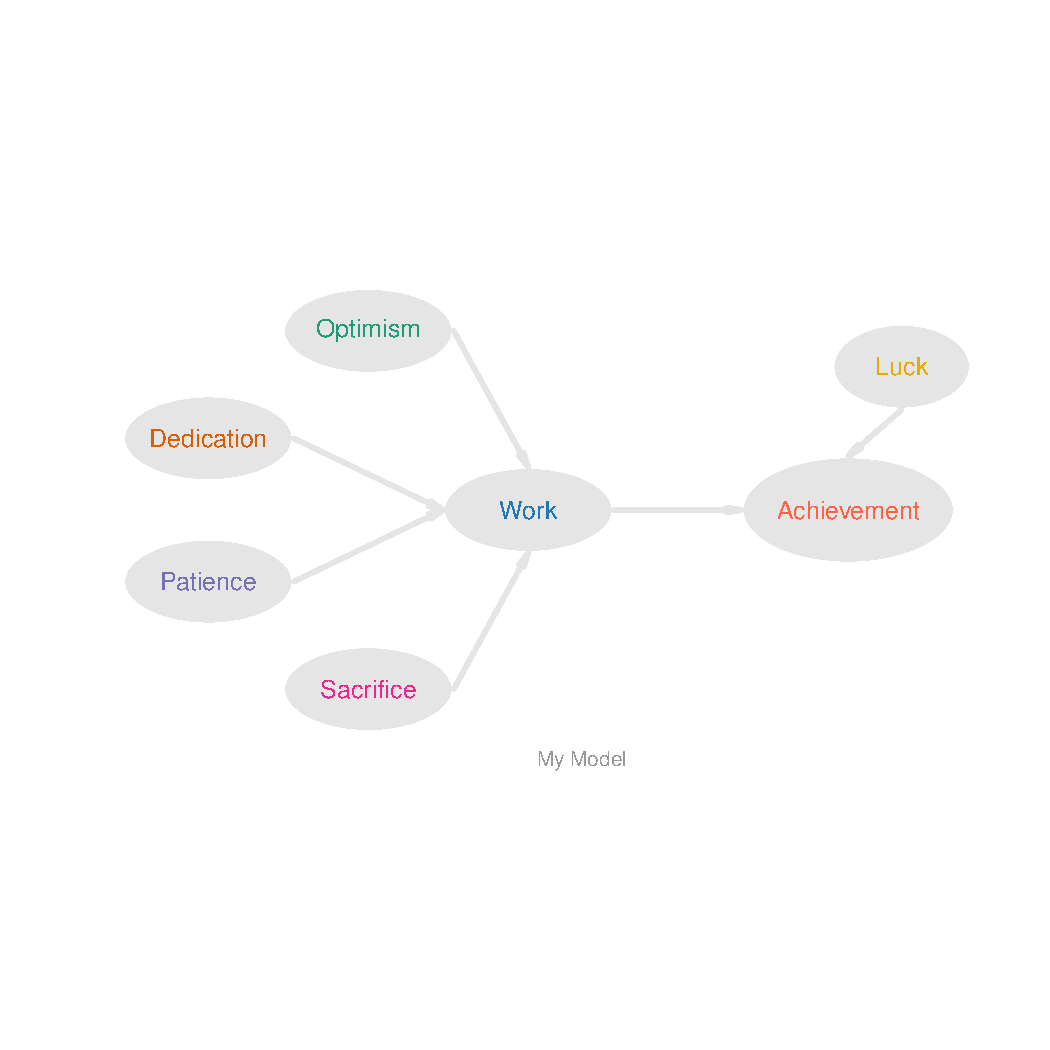
\includegraphics[width=\maxwidth]{figure/my_model} 

\end{knitrout}


% 4rd page, table of contents
%-------------------------------------------------------------------------------
\newpage
% Include dots between chapter name and page number
\renewcommand{\cftchapdotsep}{\cftdotsep}
% include the ToC
\tableofcontents



% General definitions for all Chapters
%-------------------------------------------------------------------------------

% Define Page style for all chapters
\pagestyle{fancy}
   

% Define Page style for all chapters
\pagestyle{fancy}
% Delete the current section for header and footer
\fancyhf{}
% Set custom header
\lhead[]{\thepage}
\rhead[\thepage]{}
\lfoot{\scriptsize{\textsf{\textcolor{gray}{CC BY-NC-SA 3.0 \hspace{.5mm} Gaston Sanchez}}}}
\rfoot{\scriptsize{\textsf{\textcolor{gray}{PLS Path Modeling with R}}}}




% Preface
%-------------------------------------------------------------------------------

% !Rnw root = ../PLS_Path_Modeling_with_R.Rnw


\chapter*{Preface}
\addcontentsline{toc}{chapter}{Preface}
On a sunny September morning of 2005, Tomas Aluja ---my PhD advisor--- and I were walking around the campus of the Universitat Politecnica de Catalunya in Barcelona. ``So, how did you like the symposium?'' Tomas asked me. The week before we had hosted the \textit{PLS'05 International Symposium on PLS and Related Methods}. It was my first academic conference ever and I had just been introduced to the PLS methods early that year. ``I kind of liked it'' I responded. ``What was your favorite talk?'', Tomas said. ``Well, I liked this guy's presentation and also the case study in that woman's talk'' I answered vaguely. I was part of the staff and my role during the symposium was to be in charge of one of the conference halls. In other words, I had to make sure that everything worked fine, the lights, the projector, the microphone, the speakers' banners. I barely had a chance to sit down and listen carefully to the talks. You can't blame me for not paying attention to the speakers; after all, I was checking that all the small details were in place (which I diligently did).

Tomas paused, stared at me, and put all the cards on the table: ``Would you be interested in working on PLS?'' I knew that a proposal like that from Tomas was a once-in-lifetime opportunity that I couldn't reject. ``Yes, absolutely'', I responded. I was not exactly sure if PLS was for me but I would figure that out later. ``The plan is to make an R library to calculate PLS path models. Then, we need to work on segmentation issues. You know, find a way to detect segments and compare path models \dots'' Tomas continued describing the general idea of the project, thinking out loud and mentioning some of the potential problems that I would have to deal with. When he finished, all I said was ``OK''(I'm not a very talkative person). Oh boy, what an innocent grad student I was. To put that in perspective is like if you were just start learning to climb, and then your instructor says: ``Would you be interested in Mount Everest? The plan is to climb mount Everest under the following conditions: you need to climb it by its north face, during the winter season, in alpine style, without Sherpas, with no oxygen supply, and open a new route that nobody else has climbed before''. Anyone in their right mind would thought twice about it and even then would have doubted the feasibility of the project. But I'm glad I didn't know in advance what it would take to climb ``mount PLS''. I was going to climb it or die trying.

Fast-forward to July 2009. The seemingly utopian project my advisor proposed me, became a reality. I'll save the story of what happened in those four years for when I write my memoirs. The important thing for this story was what happened on the day of my dissertation defense. That evening, after successfully defending my climbing of mount PLS, I attended the traditional dinner with Tomas, the members of the defense committee, and my invited guests. At the end when it came the time to say goodbye, Professor Ludovic Lebart, a member of my defense committee, approached me and strongly encouraged me to write a textbook about Partial Least Squares Path Modeling \textit{as soon as possible}. ``Me? A book on PLS Path Modeling? No way!'', I thought. At least not anytime soon. I smiled and told him that I would think about it. Since I had just finished my PhD, I didn't have the necessary motivation and required stamina to write another manuscript. Besides, the \textit{Handbook of Partial Least Squares} was already being edited. The world didn't need another book on PLS. Or so I thought.

Life has this strange way of proving that sometimes you are wrong. I kept maintaining the R package for PLS Path Modeling and adding more features. Emails from all over the world filled my inbox with questions, inquiries, doubts, comments, suggestions, contributions, and of course, complaints about those random but nasty, pain-in-the-butt, bugs. People asked me how to apply PLS for a given problem; how to calculate such and such; what was the meaning of those displayed numbers; and so on. Moreover, Lebart's words were still in my head. ``Maybe it wouldn't be such a bad idea to write a book on PLS Path Modeling after all'', I used to say to myself. The more I remained involved with PLS ---either by maintaining the R package, applying it for my research projects, answering emails and collaborating with other colleagues--- the more I realized there was something missing. As John Lennon said: \textit{``Life is what happens to you while you're busy making other plans''}. Finally, it was clear to me that if I didn't write this book, nobody else would. I decided not to think any more in Lebart's words, stopped making random plans, and instead made the decision to write this book about \textbf{Partial Least Squares Path Modeling} \dots \textbf{with R}. 


\section*{Why this book?}
The simplest answer to the question \textit{Why this book?} is that there are no books dedicated to instruct how to apply PLS Path Modeling using R. The extended answer is a little more complex. First, I've found the time and motivation to write it. Second, I wanted to create a resource that were different from the rest of texts about Partial Least Squares. Most of the existing literature on PLS Path Modeling consists of material describing the methodology, and showing the results from a real-life application. However, there are no resources that show readers how they can play with the broad range of PLS-PM applications using the existing software. If a grad student wants to apply a model, she has to read a paper, figure out how the authors performed the PLS-PM analysis, and then struggle with the untold steps that she might need to get her job done.

It is precisely the void in the current PLS literature with a lack of textbooks specifically dedicated to PLS Path Modeling, that I wanted to start filling. I wrote this text because I wanted to have a way to make PLS Path Modeling more accessible to a wider audience and not only to a select group of people learning PLS-PM in a seminar or workshop. If someone is interested in learning PLS-PM by herself, the path to the summit is very steep and slippery. It is one thing to work on a PhD project where it is expected that you will walk through fire to find the scant and elusive resources for your research topic. A completely different thing is to work on an analysis project without having the time, accessability and availability to books, electronic databases, journals, courses and other resources about Partial Least Squares. 

Likewise, I wanted to share my experience and knowledge on PLS Path Modeling with the users of my R package; I wanted to give them an approachable and useful book where they can find the necessary material (mostly written in plain language) to carry out their own PLS-PM analysis. This has been the toughest challenge for me. I believe that for ideas to be widely spread and adopted they need to be perceived in a friendly and understandable way. If they are perceived as obscure, arcane and intimidating, only a few people will be crazy enough to dare to apply them. PLS Path Modeling has been available since the early 1980s but went unnoticed because there were no channels of distribution. Fortunately, this has changed in the last decade, but still I want to add my own contribution. 

This book is about both the art and the science of PLS Path Modeling analysis. By this I mean that PLS Path Modeling is not only an algorithm to analyze data but also a methodology with its own mechanics and solid principles on which it is based. That is the science. But as with any other analysis, there is also human involvement and subjectivity. The idyllic perception of plugging some data in the computer, run an analysis, and get beautiful results, rarely happens in real life. All analyses require the user's skills and contextual knowledge to review the data and interpret the results. The analyses also require the user's know-how to perform an iterative process of trial an error until he or she understands what the data is telling. This is the art. 


\section*{Audience of the Book}
My hypothesized readers are a handful of senior undergraduate students, a few dozens or hundreds (or who knows, maybe more) of graduate students, and a broad variety of researchers, practitioners, and analysts that in one way or another are interested in applying PLS Path Modeling. This book assumes almost no prior experience with PLS techniques, although I imagine that you are reading this text because you have been already exposed to some PLS method. However, this text does rely on a couple of more or less technical assumptions.

It assumes you have taken introductory courses of matrix algebra and statistics. I know this is kind of naive but ideally you should have been introduced to concepts of matrix algebra like the rank of a matrix, linear (in)dependence of vectors, matrix inversion, matrix factorization, orthogonality, and eigenvectors. You should also have been introduced to basic multivariate analysis methods like regression analysis, principal component analysis, canonical correlation analysis, etc. It would also be highly desirable to have previous experience with the statistical software R. Having said that, I'm perfectly conscious that this profile is like a list of requirements that human resources people typically ask in a job posting for the ideal but imaginary candidate.

I have written the book as much informal as possible trying to keep it understandable even if you don't meet the previous assumptions. It doesn't follow a complete mathematical rigor, which I have relegated to a second plane. Instead, the discussion and explanations are more in the spirit of a tutorial. The book is designed to offer something for people who want to get started in PLS-PM, something to read as a jumping-off point for more complicated material. This does not mean that it cannot be of interest to PLS \textit{jedis} and \textit{ninjas}. However, I assume this book would be better used as your introduction to PLS Path Modeling analysis.

\paragraph{To independent readers}
My expectations is that many readers will use this book to improve the efficiency of their research, enrich their existing PLS analytical tools, and develop the skills needed for new types of studies. Much of what I use in practice was garnered through self-directed experience, and I have tried to compile this knowledge in one place to make it easier for other analysts to do the same.

\paragraph{To teachers using this book}
Although this book is written to stand on its own outside the classroom, it is also been designed to be used as a supplement text within the classroom. I actually don't know how many courses about PLS-PM are out there in the academic world, but I do know that many seminars and workshops on PLS-PM and related methods are taught in an increasing number every year. While there are examples and opportunities for practicing new skills as they are developed, there are no formal exercises or test questions in this book.




\section*{Beyond this book}
A lot of things have happened since that September of 2005. In particular, PLS Path Modeling has become much more popular while its community has grown substantially, and this trend is not going to slow down anytime soon. 

This is the book that I wish existed when I started working on PLS in 2005. My aim in writing this book has been to allow more people to get into the PLS path modeling world. It is also intended as a stepping-stone to more advanced topics. The long-term goal is to empower you in the use of PLS and enjoy the rewards that it brings. It is my hope that by showing users how to apply the powerful PLS tools, they will be free to spend more time on the pleasures of scientific inquiry and data analysis projects. I hope you find it useful and are able to apply its content in your work and research projects. I certainly enjoyed the challenge of putting the book together.

To comment or ask technical questions about this book, send an email to: \\
\texttt{gaston.stat at gmail.com}


\section*{Attribution}
This work is licensed under a Creative Commons Attribution-NonCommercial-ShareAlike 3.0 Unported License. You can check the details at: \\
\href{http://creativecommons.org/licenses/by-nc-sa/3.0/}{http://creativecommons.org/licenses/by-nc-sa/3.0/}

In essence it states that I retain the Copyright but you are free to use, copy, reproduce and distribute the material in this book, but only under the same license to this one. You may not alter, transform, build upon it, or use this work for commercial purposes. However, permission to use this book in nonprofit teaching is still granted, provided the authorship and licensing information here is displayed. If you are using the book, either in teaching a class or for your own learning, I would highly appreciate your letting me know.

I will be ridiculously happy and utterly pleased if you give proper attribution to my work. I'm not asking you for money or any donations; I'm not asking you to like me on any annoying social network; I'm not asking you to register or fill any stupid form. I'm just simply asking you to give me credit for my work. It costs you nothing, it doesn't hurt you, and I guarantee you that I would do the same for you. Also, it'll give you instant credit in your karma balance. Here's how you can cite my book:
\vspace{2mm}
\begin{quotation}\noindent
\textsf{Sanchez, G. (2013) \textbf{PLS Path Modeling with R} \\
Trowchez Editions. Berkeley, 2013.} \\
\hspace{1.5mm} \texttt{http://www.gastonsanchez.com/PLS\_Path\_Modeling\_with\_R.pdf}
\end{quotation}
\vspace{2mm}
See how easy that is? \\


\vspace{2mm}
Gaston Sanchez \\
Berkeley, California. \\
January 2013.


% Set arabic (1,2,3...) page numbering
\pagenumbering{arabic}

% If the chapter ends in an odd page, you may want to skip having the page
%  number in the empty page
\newpage
\thispagestyle{empty}
\mbox{}


% Chapter1

% !Rnw root = ../PLS_Path_Modeling_with_R.Rnw


\chapter{Introduction}
This book provides a hands-on introduction to Partial Least Squares Path Modeling using the R package \plspm{}. Although there are a few texts that cover the theoretical aspects of PLS Path Modeling (PLS-PM) with some applications to real data, there are virtually no textbooks that teach how to use PLS Path Modeling and how to handle its broad range of applications with the existing PLS-PM software. The goal of this book is to introduce you to the world of PLS-PM using \plspm{} and \textbf{R} through practical examples; teach you the basics so that you can analyze your own data; and even turn you into a confident PLS-PM user who can try out different analysis options.


\section{PLS Path Modeling}
Let's face it once and for all: \textit{Partial Least Squares Path Modeling} is a name that does not provide many clues about what it is or what it can do. Simply put, Partial Least Squares Path Modeling is a statistical data analysis methodology that exists at the intersection of Regression Models, Structural Equation Models, and Multiple Table Analysis methods. If you were to review the extensive literature about PLS Path Modeling, chances are that you would find some variation of the following descriptions:

\begin{itemize}
 \item PLS-PM is the Partial Least Squares approach to Structural Equation Modeling.
 \item PLS-PM is a statistical method for studying complex multivariate relationships among observed and latent variables.
 \item PLS-PM is a data analysis approach for studying a set of blocks of observed variables in which each block can be summarized by a latent variable and that linear relations exist between latent variables.
\end{itemize}

The first description above is the most common on PLS Path Modeling. In most cases, PLS Path Modeling is usually referred to as the PLS approach to Structural Equation Modeling (SEM). However, around the small but growing PLS community, the term Path Modeling is preferred over Structural Equation Modeling, although both terms are often used interchangeably. My preferred description is the one that views PLS-PM from a broader conceptual perspective for analyzing multiple relationships between blocks of variables. Under this framework, we establish the relationships among the blocks by taking into account some previous knowledge (e.g. theory) of the phenomenon under analysis. In addition, we assume that each block of variables plays the role of a theoretical concept represented in the form of a latent (unobserved) variable.

Personally, I try to avoid using the term SEM for two main reasons. The first reason has to do with the connotations behind Structural Equation Modeling where the dominating approach is based on Covariance Structure Analysis (sometimes also referred to as LISREL). Because of the overwhelming market share of LISREL, PLS-PM occupies a small niche within the SEM community. For the same reason, CSA purists perceive PLS-PM as an awkward methodology that distorts the SEM ideals (for the record, I have nothing against the CSA community and the \textit{Lisrelites}). The second reason has to do with the broad range of applications outside the SEM spectrum that can be targeted with the flexible PLS-PM standpoint. 

Though I don't use SEM often, I sometimes may use the term SEM-PLS because it helps people to have some reference that allows them to get a better idea of the method. What I prefer to use is the term \textbf{PLS Path Modeling} to give the methodology its own territory. Yes, you can apply PLS for SEM applications, but there are also many other types of problems that can be treated via PLS-PM that don't fit within the SEM framework.


\subsubsection*{The Network Analogy}
It is not easy to explain PLS Path Modeling in simple terms to newcomers but I'll give my best shot. First, imagine that you have a network of variables. Usually, the connections in the network are assumed to represent some cause-effect process. But you can think of it as a flow chart where the process flows in one direction (no loops allowed). Having defined the network, one of the goals is to quantify the connections or relationships among the variables. 

The interesting part comes with the subtlety that each of the connected variables are obtained by combining a set of other variables. Although this is the interesting part it is also the tricky part, but the main idea to keep in mind is the network of connected variables. PLS Path Modeling quantifies the relationships by considering the network as a \textit{system of multiple interconnected linear regressions}. Still don't get it? That's why I wrote this book as my bold yet humble attempt to help people not only understand Partial Least Squares Path Modeling but also to show them how to apply it in R. 



\section{R package \plspm{}}
R is a free open source software for data analysis, statistical computing, and graphics. In turn, \plspm{} is an R package dedicated to Partial Least Squares Path Modeling analysis. The \plspm{} project timidly began in the fall of 2005 as part of my PhD work. One of the initial goals was to create a package to estimate PLS path models in R. Almost four years later, the first R package for PLS-PM was created and the first version was released on April, 2009. Two months later, with the collaboration of Laura Trinchera, REBUS-PLS for detecting classes was added to \plspm{}. Since then, various features and new capabilities have been implemented in the package, and its development continues every year.

There are a number of other softwares for PLS Path Modeling: perhaps the most well known are \textit{SmartPLS} (by Christian Ringle, Sven Wende and Alexander Will) and the PLSPM module from \textit{XLSTAT} (by Addinsoft). In addition, there's also \code{semPLS} which is another R package (by Armin Monecke). 

One of the main differences of \plspm{} to other PLS-PM software is the lack of a graphical interface to draw path diagrams. This may be a surprise for readers that are used to working with other programs in which you are able to define a model with a combination of mouse clicks and dragging objects. While \plspm{} might not be the optimal choice if what you're looking for is using a mouse to define the models, it does not mean that it is less advantegeous. On the contrary, you will be surprised by how fast it is to define a model and run a PLS-PM analysis with \plspm{}. The other major difference is that you need to know a little bit about R and feel comfortable typing commands. But this is precisely what makes \plspm{} stronger by taking full advantage of the data analysis options and programming capabilities of R. 


\subsection{Why R?}
The main reason for choosing R is that it is an extremely powerful program for manipulating and analyzing data. R's unstoppable popularity has made it \textit{the} software for statistics and analytics in many disciplines, and it is increasingly taught at many universities. The second major reason for selecting R is that it's platform independent ---you can use it under Windows, Mac or Unix--- And is free. You don't have to spend a cent in licenses, renew contracts, negotiate upgrades, or pay for maintenance. Commercial software vendors may provide support and offer some type of guarantee, but that's secondary. You just can't beat the price and functionality of R.

R is enriched by the fact that many people (me among them) from all over the world contribute and share their own work in the form of packages for almost whatever method you can think of. No other commercial software has that advantage of offering the latest state-of-the-art methods. Likewise, R has unrivaled help resources, both online and physical. There are many online forums, email lists, interest groups, forums, blogs, and websites full of rich information about R. In addition, many R books of excellent quality are increasingly published every year. What I really value about R is that it is open source: you can see the guts of the code. It's not a black box, so you can actually see what's behind the functions you are using. In addition, being a free software, R has no rival for reaching the marginalized academic places of the world. Just think about those students, professors and researchers from developing countries that would be left further behind without resources such as R. As the Spanish say, \textit{bueno, bonito y barato}, which means ``good, beautiful and inexpensive'', Why use anything else?




\section{About Partial Least Squares}
You have probably heard the term \textbf{Partial Least Squares} a few times before reading this book. If you are like me, those three words might be intimidating the first time you hear them. You are probably familiar with \textit{least squares}, but what about the \textit{partial}? Partial Least Squares even sounds like a spell out of Harry Potter's world. 

So, what exactly is Partial Least Squares? Well, it depends on who you talk to. Perhaps the most popular answer is to equate PLS as a regression analysis technique. This is too narrow and somewhat misleading, especially because there are so many methods, techniques, and algorithms that share this brand. It is true that PLS has to do with regression analysis but it is much more than that. From the broadest point of view, PLS is a family ---I would say a big family--- of data analysis methods. However, this is perhaps the main obstacle to defining what PLS is. These methods are designed for dealing with a wide range of data analysis tasks such as exploration, visualization, explanation, prediction, classification, and study of structural systems. In its purest data analysis sense, PLS can be viewed as a set of methods for analyzing multiple relationships between various blocks of variables (or tables of data). If we consider a block of variables as a data table, the difference between the various PLS methods depends on the number of tables and the type of relationships between variables.

The perception of PLS methods is not exempt of misconceptions, misunderstandings, and misinterpretations. One initial obstacle has to do with the terminology and jargon: \textit{latent structures}, \textit{projections}, \textit{component-based}, \textit{soft modeling}, \textit{scores}, \textit{loadings}, \textit{path coefficients}, \textit{path diagrams}, just to mention a few terms. There is also a widespread use of acronyms: PLS, PLSR, PLSPM, NIPALS, and many more. However, once you have surpassed the initial phase of adaptation, PLS methods open a new way of dealing with many statistical problems. Think of PLS like a set of tools that you can use for different purposes. Well applied, PLS can be a very handy and useful set of tools. However, you have to keep in mind that there is no single best approach to analyze data, and there is also no single method that works for all problems. PLS is not the exception. In this sense, PLS data analysis is both an art and a science that require not only mathematical principles, but it also requires some intuition and skills that are developed over time with practice. 



\subsection{Short tale of PLS}
I have dedicated an entire appendix at the end of the book to the historical overview of PLS Path Modeling. However, let me offer you a brief summary to start making things a bit more clear. The development of PLS methods as we know them took place over a period of approximately 20 years. Its origins can be traced back to the mid 1960s where the first PLS analytical tools were developed by Herman Wold at the Uppsala University, Sweden. Throughout the 1970s, Wold's team refined and polished different techniques that gave rise to a series of methods more or less unified under a common umbrella: a set of approaches whose estimation was based on iterative algorithms of least squares regressions. Briefly, Herman Wold and his group developed PLS as a multi-tool to handle different types of problems that could be solved by applying least squares. In other words, rather than a single technique, the set of PLS methods was developed as a toolkit to tackle several data analysis problems and solving them by applying a number of adapted least squares procedures.

In the 1980s, the evolution of the PLS methods experienced an interesting metamorphosis led by Svante Wold (son of Herman Wold) with the application of the PLS principles to the analysis of chemical data. Prior to this event, the application of PLS methods was focused on economics and social sciences without really catching the attention of social researchers and related practitioners. However, the application to chemical data opened an unexplored venue for some of the PLS tools and were quickly accepted with great success. This developmental branch took the shape of the techniques associated to what is known as PLS Regression.

Not all of the PLS tools shared the same luck as the PLS Regression techniques. During the 1990s, the less successful PLS Path Modeling (PLS-PM) approach remained in an almost complete oblivion. Fortunately, PLS-PM was kept active by a handful of practitioners, mainly in the USA, saving it from extinction. Then, in the late 1990s, PLS Path Modeling caught the attention of a group of european statisticians and analysts under guidance of Michel Tenenhaus. With an authentic curatorial task, they slowly repositioned the general framework of PLS methods on the data analysis map.    

In the last decade (2000-2010), the PLS analysis methods were subjected to a great effort of international diffusion which continues today. As a result, new proposals and developments have been appearing in all the different PLS areas. In addition, several programs and multiple software have been released that allow users to apply the variety of PLS related methods. This reflects their great modeling potential, versatility, and analytical capabilities. 



\subsection{Regressionists and Path-modelists}
Nowadays, there are two main populations within the PLS world. PLS users can be roughly separated in two populations, let me call them: the \textit{regressionists} and the \textit{path-modelists}. The regressionists are comprised by users of PLS regression methods. The path-modelists are related to Path Modeling approaches (SEM and multiple table analysis). Of course, this is a simplistic view, but reflects what I've seen in congresses, seminars, talks, and in the PLS literature. You are either identified as a regressionist or as a path-modelist. The regressionists typically work with bio-chemical and life sciences data that involve analytical problems from disciplines such as chemometrics, sensometrics, and biometrics in general. In constrast, the path-modelists usually work with data from social siences like psychometrics, marketing, information technology, and economics.

I was introduced to PLS techniques from a regressionist standpoint but got involved with the path-modelists for my PhD research. I suppose that makes me one of those rare hybrids in the middle of both traditions. Although both groups try to take ownership of the brand name PLS, I prefer to be generalist, looking at the forest instead of the trees. It's undeniable that the projects you get involved with, the fields of research you work in, and the type of data you analyze, shape you as a regressionist or as a path-modelist. But you don't have to take party for one group and break links with the other.




\section{Structure of the book}
Although this book is an introductory book for PLS Path Modeling it is not a comprehensive reference nor the definitive PLS-PM book; for that there are great resources written by PLS gurus that describe the bells and whistles of PLS. This book can be divided in two major parts. Part I (Chapters 2 - 5) sets the fundamentals of PLS Path Modeling and is organized as a progressive series of topics, each designed to build upon concepts introduced earlier. This first part follows a concise learning path that is essential for a firm grasp on PLS Path Modeling. Part II (Chapters 6 - 9) covers topics at the next level in the PLS-PM learning scale. The chapters in the second part are self-contained and you could read them independently from one another or in a different order than the way they are numbered.

\paragraph{Part I}
\begin{enumerate}[leftmargin=*]
 \item[] \textbf{Chapter 2} provides the essentials you need to know about PLS Path Modeling. A basic hands-on introduction is also provided on how to perform a PLS-PM analysis with \plspm{}
 
  \item[] \textbf{Chapter 3} introduces the theoretical framework behind PLS-PM and describes the model specifications as well as the algorithm. 
  
  \item[] \textbf{Chapter 4} describes how to interpret and diagnose the results from a PLS-PM analysis, specifically with the output provided by \plspm{}.

  \item[] \textbf{Chapter 5} shows you how to run a PLS-PM analysis from beginning to end with an adapted model on customer satisfaction applied to educational services.
\end{enumerate}

\paragraph{Part II}
\begin{enumerate}[leftmargin=*]
  \item[] \textbf{Chapter 6} introduces the topic of comparing groups in PLS Path Modeling, and describes two common approaches for comparing two models: 1) the bootstrap $t$-test, and 2) the permutation test.

  \item[] \textbf{Chapter 7} describes testing moderating effects with three types of approaches: 1) product-indicator, 2) two-stage approach, and 3) categorical variable approach.

  \item[] \textbf{Chapter 8} describes higher-order contructs with three methods: 1) repeated indicators approach, 2) two-step approach, and 3) hybrid approach.

  \item[] \textbf{Chapter 9} is dedicated to the issue of detecting classes with the REBUS methodology.
  
  \item[] \textbf{Appendix A} contains a historical overview of PLS-PM

\end{enumerate}





\section{R and \plspm{}}
This book assumes that you have familiarity with the software environment \textbf{R}. The official website of the R project, \texttt{\href{http://www.r-project.org}{www.r-project.org}}, is the best place to look for information about R. It includes links to the Comprehensive R Archive Network, better known as \textbf{CRAN}, where you can download R. Since R is available for Linux, MacOS X, and Windows, there is no excuse for not installing it. 

Although I'm assuming that you have some knowledge on how to work with R, I'm going to begin with some basics on how to start using the R language. For information on downloading and installing R check the CRAN webpage: \\ \texttt{\href{http://cran.r-project.org}{http://cran.r-project.org}}. 

If you come across any problem or if you want to know more about the installation process, you can look for tutorials in youtube and/or ask google (or your preferred search engine).

R comes with a bunch of stuff, including a simple graphical user interface (GUI). Now, if you were expecting a highly visual interface and drag-and-drop features, I'm afraid you will be disappointed. Instead, what you get with the GUI is both the R environment and the R console at the same time. This means that you have to type commands in. In the CRAN website you have a variety of contributed documentation at: \\ 
\texttt{\href{http://cran.r-project.org/other-docs.html}{http://cran.r-project.org/other-docs.html}}

For R newbies and rookies good places to start are: 
\begin{itemize}
 \item R for Beginners (by Emmanuel Paradis) \\ 
 \texttt{\href{http://cran.r-project.org/doc/contrib/Paradis-rdebuts\_en.pdf}{http://cran.r-project.org/doc/contrib/Paradis-rdebuts\_en.pdf}}
 \item Kickstarting R (compiled by Jim Lemon) \\ 
 \texttt{\href{http://cran.r-project.org/doc/contrib/Lemon-kickstart/index.html}{http://cran.r-project.org/doc/contrib/Lemon-kickstart/index.html}}
\end{itemize}

There is no single best solution for working with R. Some people may prefer to work with R from the command line. Others might be perfectly happy working with the default GUI that comes with the versions for windows or Mac. I learned R the hard way by using a text editor with no syntax highlighting and worked like that for seven years. But you don't have to be a stubborn martyr like me. Be smart and use one of the free \textit{integrated development environments} (IDE) developed for R. Here are some interesting IDEs that you can explore:
\begin{itemize}
 \item RStudio \texttt{\href{http://www.rstudio.org}{http://www.rstudio.org}}
 \item StatET \texttt{\href{http://www.walware.de/goto/statet}{http://www.walware.de/goto/statet}}
 \item ESS (Emacs Speaks Statistics) \texttt{\href{http://ess.r-project.org}{http://ess.r-project.org}}
\end{itemize}
I use RStudio and I couldn't be happier (not to mention more productive) I highly recommend it. But you can use whatever other IDE fits your needs and preferences.

New versions of R are released every six months, once in April and again in October. This is important to know because from time to time you must update your R version.


\subsubsection*{Installing packages}
By default, R comes with many packages (a.k.a. libraries) that allow you to perform a variety of analysis and tasks. However, there are many other additional R packages that don't come with the default version but that you will probably want to add. To install a package we use the function \texttt{install.packages()}. For instance, to install the package \code{colortools}, open R and type in your R console:
\begin{knitrout}
\definecolor{shadecolor}{rgb}{0.969, 0.969, 0.969}\color{fgcolor}\begin{kframe}
\begin{alltt}
\hlcomment{# installing colortools (this is a comment!)}
\hlfunctioncall{install.packages}(\hlstring{"colortools"})
\end{alltt}
\end{kframe}
\end{knitrout}

When you install a package you will have to choose a CRAN mirror, so choose one that is closest to your geographical location. What we are doing with the function \texttt{install.packages()} is saying that we want to install the package \code{colortools}. Note that comments are indicated with the symbol \#, that is, anything that appears after \# won't be executed. I use comments a lot and you will see that almost all the R commands in this book have their corresponding comments. In this way you can better read the R code and understand what I'm doing.

Once a package has been installed, you need to load it in your current R session. To do this, use the function \texttt{library()} and call it like this:
\begin{knitrout}
\definecolor{shadecolor}{rgb}{0.969, 0.969, 0.969}\color{fgcolor}\begin{kframe}
\begin{alltt}
\hlcomment{# loading colortools (this is another comment!)}
\hlfunctioncall{library}(colortools)
\end{alltt}
\end{kframe}
\end{knitrout}


For those readers using R for the first time, you should know that R is case-sensitive. This means that the commands in this book should be entered exactly, using the same capital (uppercase) and small (lowercase) letters provided in the examples. If a command is \code{library} (lowercase) but you type \code{Library} or \code{LIBRARY}, it will not work.



\subsection{Installing \plspm{}}
\plspm{} is an R package for performing Partial Least Squares Path Modeling (PLS-PM) analysis. \plspm{} is available for free on CRAN at: \\ 
\texttt{\href{http://cran.r-project.org/web/packages/plspm/index.html}{http://cran.r-project.org/web/packages/plspm/index.html}}.

The main version of the package is the one hosted in CRAN. Install it like you would install any other package in R by using the function \code{install.packages()}:
\begin{knitrout}
\definecolor{shadecolor}{rgb}{0.969, 0.969, 0.969}\color{fgcolor}\begin{kframe}
\begin{alltt}
\hlcomment{# installing the package 'plspm'}
\hlfunctioncall{install.packages}(\hlstring{"plspm"})
\end{alltt}
\end{kframe}
\end{knitrout}


Once \plspm{} has been installed, you can use \code{library()} to load the package: 
\begin{knitrout}
\definecolor{shadecolor}{rgb}{0.969, 0.969, 0.969}\color{fgcolor}\begin{kframe}
\begin{alltt}
\hlcomment{# load package 'plspm'}
\hlfunctioncall{library}(\hlstring{"plspm"})
\end{alltt}
\end{kframe}
\end{knitrout}


\plspm{} comes with a number of functions that perform various types of analysis. The main function, which has the same name as the package, is the function \fplspm{} that is designed for running a full PLS-PM analysis. In this book \plspm{} refers to the R package and \fplspm{} refers to the function.

For a description of \fplspm{} and its arguments, use the function \code{help()} like so:
\begin{knitrout}
\definecolor{shadecolor}{rgb}{0.969, 0.969, 0.969}\color{fgcolor}\begin{kframe}
\begin{alltt}
\hlcomment{# asking for help about function plspm}
\hlfunctioncall{help}(plspm)
\end{alltt}
\end{kframe}
\end{knitrout}

When you use the function \code{help()} a window with documentation about the topic you are asking help about for will open. This documentation is the information contained in the technical manual of the package and is also available in pdf format at: \\
\texttt{\href{http://cran.r-project.org/web/packages/plspm/plspm.pdf}{http://cran.r-project.org/web/packages/plspm/plspm.pdf}}

More friendly documentation and tutorials about \plspm{} can be found at: \\
\texttt{\href{http://www.gastonsanchez.com/plspm}{www.gastonsanchez.com/plspm}}. 

\plspm{} is still evolving; ongoing refinements, new features and fixing bugs are being enhanced regularly. Even as this book was being written, \plspm{} has evolved, and you can expect it to keep doing so.




\subsection{Some Extra Details}
Although most of the case studies in this book are simple examples, all the data used is real and the models should be fairly applicable. The hypotheses, the relationships, and the conceptualizations behind every model are mine and you shouldn't take them as the final word. You might agree or disagree with my conclusions and interpretation of the results. That's fine with me; we can sit down and order a beer or a coffee to discuss the material in more detail. For this book at least, the journey is more important than the results.

\paragraph{Data for Examples:} Almost all the data for the case studies in the book come with the package \plspm{}. This means they are already available and you don't need to import anything. There is only one case study where you need to download a data set and import it in R (see Chapter 5).

\paragraph{Code Examples:} Most of the code examples in the book are shown with input and output in a highlighted format like this one:
\begin{knitrout}
\definecolor{shadecolor}{rgb}{0.969, 0.969, 0.969}\color{fgcolor}\begin{kframe}
\begin{alltt}
\hlcomment{# stupid example}
x = 2
y = 3
\hlcomment{# sum}
z = x + y
\hlcomment{# easy peasy}
z
\end{alltt}
\begin{verbatim}
## [1] 5
\end{verbatim}
\end{kframe}
\end{knitrout}

Much of the code in the examples reflects my personal taste for working with R, which might not be the same as yours. Also, I've chosen clarity over shortness and efficiency. Many of the examples could be executed in a more synthesized or efficient way. However, I decided to use relatively verbose code to help explain how things are done. I prefer to use two or three times more lines of code, writing function arguments explicitely, and commenting the main steps, to try to help readers understand what I'm doing.


\paragraph{R style flavors}
There have been efforts of different groups to establish some style guidelines and advices for writing code in R. One of the most popular flavors is the Google's R Style Guide available at: \\
\texttt{\href{http://google-styleguide.googlecode.com/svn/trunk/google-r-style.html}{http://google-styleguide.googlecode.com/svn/trunk/google-r-style.html}} \\
According to Google's guidelines (and many other authors), I should use the assignment symbol \code{'<-'} instead of the equal symbol \code{'='}. 
\begin{knitrout}
\definecolor{shadecolor}{rgb}{0.969, 0.969, 0.969}\color{fgcolor}\begin{kframe}
\begin{alltt}
\hlcomment{# I used to do this}
x <- 3
\hlcomment{# now I do this}
y = 3
\end{alltt}
\end{kframe}
\end{knitrout}

I do not regard the symbol \code{'='} as bad for assignment, but you can use whatever you like. 

\paragraph{About this book}
This textbook was entirely written using the \code{Sweave} and \code{knitr} ``combo'' with RStudio. \code{Sweave} is an R package developed by Friedrich Leisch that allows to embed the R code for complete data analyses in LaTeX documents. \code{knitr} is an R package developed by Yihui Xie that allows you to produce dynamic reports with R while adding more capabilities to \code{Sweave}. RStudio supports the powerful and flexible system of \code{Sweave} and \code{knitr} for creating dynamic reports and reproducible research using LaTeX.

I know that R can be tricky to learn and, unless you are a programming geek, will take you some time to get used to. But the good news is that you should be able to reproduce all the examples in your machine by simply copy-pasting the R code in this book. In this way, you learn how to apply PLS-PM methods using some bits of text and code in R. Of course, you'll be most successful with this book if you have some familiarity with R.





\section{Reading List}
Instead of having a long boring list of references at the end of the book, I've decided to provide at the end of every chapter a suggested reading list with the main references of the discussed material. So here is the reading list for the content in this chapter.

\paragraph{Books on PLS Path Modeling}
There are many resources about PLS Path Modeling: articles, papers, special editions of journals, book chapters, encyclopedia's entries, symposium proceedings, textbooks, handbooks, and websites. The following books are my suggestion of resources that talk about PLS in general. In the next chapters I will offer other references depending on the topic we are discussing.

\begin{itemize}
 \vspace{2mm}
 \item \textbf{\textsf{Handbook of Partial Least Squares}} edited by Esposito Vinzi V., Chin W.W., Henseler J., and Wang H. (2010). As part of the Springer Handbooks series on computational statistics, this volume gives a comprehensive overview of PLS methods with an emphasis on Marketing applications. If you can aford it, it's worthwhile the investment.
 
 \vspace{2mm}
 \item \textbf{\textsf{La R\'{e}gression PLS: Th\'{e}orie et Pratique}} by Michel Tenenhaus (1998). This would be \textit{the} best-selling PLS book \dots if it wasn't written in French. It's the ideal textbook for a PLS course for French speakers and a good excuse to start learning French.
 
 \vspace{2mm}
 \item \textbf{\textsf{Systems under indirect observation: causality, structure, prediction. Vol II}} edited by Karl Joreskog and Herman Wold (1982). If you can have access to this book with green cover you must definitely check it out. Perhaps the only compendium by Wold \textit{et al} with all the material of what we would officially call PLS Path Modeling.
\end{itemize}


\paragraph{Books on R}
As with PLS-PM resources, the same can be said about R, although there is much more material about R than PLS-PM. My recommended list of books is for readers that have little or no experience with R. These are in my opinion good textbooks that will help you gain and improve your R data manipulation skills.

\begin{itemize}
 \vspace{2mm}
 \item \textbf{\textsf{Beginning R: An Introduction to Statistical Programming}} by Larry Pace (2012). A hands-on book showing how to use the R language, write and save R scripts, build and import data files, and more.

\vspace{2mm}
 \item \textbf{\textsf{A Beginners's Guide to R}} by Alain F. Zuur, Elena N. Ieno, and Erik Meesters (2009). The text covers a variety of tasks that can sometimes frustrate beginners: how to download and install R, import and manage data, elementary plotting, an introduction to functions, and common beginner mistakes.
 
 \vspace{2mm}
 \item \textbf{\textsf{Using R for Data Management, Statistical Analysis and Graphics}} by Nicholas J. Horton and Ken Kleinman (2011). This book covers many common tasks such as data management (how to get your data in R), how to summarize and get descriptive statistics.

 \vspace{2mm}
 \item \textbf{\textsf{Data Manipulation with R}} by Phil Spector (2008). This book presents a wide array of methods applicable for reading data into R, and efficiently manipulating of data.
\end{itemize}


% Chapter2

% !Rnw root = ../PLS_Path_Modeling_with_R.Rnw


\chapter{Getting Started with PLS-PM}
In this chapter we will cover the basic concepts that are essential for a firm grasp on PLS Path Modeling. Rather than jumping into the technical aspects of the PLS-PM algorithm, I prefer to give a hands-on introduction with a simple yet interesting example of how to apply PLS-PM. The objective is to set the stage so that you are prepared for the content discussed in the rest of the book. The theoretical details and the nitty-gritty of the PLS-PM engine will wait until the next chapter. I have tried to keep everything as simple and understandable as possible. But at the same time, I have tried to cover as many aspects as possible, especially from the Structural Equation Modeling point of view. However, I have taken the liberty of allowing me a number of descriptions that don't necessarilly satisfy the formal material discussed in other textbooks.



\section{Case Study: Index of Success}
For this example our goal will be to obtain an \textit{Index of Success} using data of Spanish professional football teams. The data comes from the professional Spanish Football League, \textit{La Liga}, and it consists of 14 variables measured on 20 teams. I collected and manually curated data from the 2008-2009 season from different websites like \textit{LeagueDay.com}, \textit{BDFutbol}, \textit{ceroacero.es}, \textit{statto.com} and \textit{LFP}. The resulting dataset comes with the package \plspm{} under the name \texttt{spainfoot}. To get access to the data, you must first call the package \plspm{} and then use the function \code{data()} in your R console:



\begin{knitrout}
\definecolor{shadecolor}{rgb}{0.969, 0.969, 0.969}\color{fgcolor}\begin{kframe}
\begin{alltt}
\hlcomment{# load package plspm}
\hlfunctioncall{library}(plspm)

\hlcomment{# load data spainfoot}
\hlfunctioncall{data}(spainfoot)
\end{alltt}
\end{kframe}
\end{knitrout}


To get an idea of what the data looks like we can use the \texttt{head()} function which will show us the first \texttt{n} rows in \texttt{spainfoot}
\begin{knitrout}
\definecolor{shadecolor}{rgb}{0.969, 0.969, 0.969}\color{fgcolor}\begin{kframe}
\begin{alltt}
\hlcomment{# first 5 rows of spainfoot}
\hlfunctioncall{head}(spainfoot, n = 5)
\end{alltt}
\begin{verbatim}
##            GSH GSA  SSH  SSA GCH GCA  CSH  CSA WMH WMA LWR LRWL
## Barcelona   61  44 0.95 0.95  14  21 0.47 0.32  14  13  10   22
## RealMadrid  49  34 1.00 0.84  29  23 0.37 0.37  14  11  10   18
## Sevilla     28  26 0.74 0.74  20  19 0.42 0.53  11  10   4    7
## AtleMadrid  47  33 0.95 0.84  23  34 0.37 0.16  13   7   6    9
## Villarreal  33  28 0.84 0.68  25  29 0.26 0.16  12   6   5   11
##             YC RC
## Barcelona   76  6
## RealMadrid 115  9
## Sevilla    100  8
## AtleMadrid 116  5
## Villarreal 102  5
\end{verbatim}
\end{kframe}
\end{knitrout}


The description of each variable is given in the following table:

\begin{table}[h]
 \caption{Description of variables in data \code{spainfoot}} 
 \centering
 \begin{tabular}{l l}
  \hline
  Variable & Description \\
  \hline
  \code{GSH} & total number of goals scored at home  \\
  \code{GSA} & total number of goals scored away \\
  \code{SSH} & percentage of matches with scores goals at home \\
  \code{SSA} & percentage of matches with scores goals away \\
  \code{GCH} & total number of goals conceded at home \\
  \code{GCA} & total number of goals conceded away \\
  \code{CSH} & percentage of matches with no conceded goals at home \\
  \code{CSA} & percentage of matches with no conceded goals away \\
  \code{WMH} & total number of won matches at home \\
  \code{WMA} & total number of won matches away \\
  \code{LWR} & longest run of won matches \\
  \code{LRWL} &longest run of matches without losing \\
  \code{YC} & total number of yellow cards \\
  \code{RC} & total number of red cards \\
  \hline
 \end{tabular}
 \label{tab:spainfoot}
\end{table}


\subsection{Of latent and manifest variables}
One of the most common applications of PLS Path Modeling is the calculation of indices to quantify some key concept or notion of importance. Common PLS examples of indices may include \textit{Index of Satisfaction}, \textit{Index of Motivation}, \textit{Index of Usability}, or in our case an \textit{Index of Success}. The issue with these four concepts (\textit{satisfaction}, \textit{motivation}, \textit{usability}, \textit{success}), is that they are things that cannot be measured directly. I could ask you how satisfied you were with the food you had in the last restaurant you visited. Or I could ask you how motivated you were to start reading this book. But even though I could ask you those questions, that doesn't mean I'm able to measure your satisfaction or your motivation. In fact, I'm not sure whether I would ever be able to measure such things, at least in a precise quantitative form. I cannot take a blood sample from you and measure your level of satisfaction; there is no device like a thermometer or a baumanometer that I can use to measure the amount of motivation you have. However, I can use a set of other questions that in some way reflect how happy or how sad you are, and then combine this information and summarize it to create an \textit{index of satisfaction}. Likewise, I can gather information about the results of the matches played by the Spanish teams, and then combine it to get an \textit{index of success}.


\subsubsection*{Latent Variables}
As you can imagine, \textit{satisfaction}, \textit{motivation}, \textit{usability} and \textit{success} are only four examples of an infinite number of other concepts that cannot be measured directly. Admittedly, sometimes we must face the fact that the variables of interest in our models cannot be observed nor measured directly. These concepts receive the special name of \textbf{latent variables} but they are also known as constructs, composites, hypothetical variables, theoretical concepts, intangibles, and factors.

These variables are very common in social sciences and behavioral sciences (e.g., psychology, sociology, economy) in which there are many concepts of theoretical nature. For instance, psychologists speak of \textit{intelligence}, \textit{commitment}, and \textit{self-esteem}. Sociologists refer to \textit{social structure}, \textit{social stratification}, and \textit{social status}. Economists speak of \textit{utility}, \textit{economic development}, and \textit{organizational performance}. But we can also find unobserved entities in the biological sciences. For example, in ecology we might encounter concepts like \textit{soil fertility}, \textit{territory quality}, and \textit{habitat structure}.

The interesting part is that when we work with theoretical concepts and constructs (i.e., developing theories and models) we tend to conceive expected causal relationships on them. For example, let's consider the following actions:
\begin{itemize}
 \item A marketing manager proposes new return policies to increase \textit{customer satisfaction}.
 \item A group of high school teachers decide to increase the extracurricular activities to improve students' \textit{academic achievement}.
 \item A scientist suggests planting native flowers to regenerate the \textit{habitat structure} of pollinator insects.
 \item A coach establishes a training scheme to improve the \textit{defensive performance} of his team.
\end{itemize}

\vspace{2mm}
The actions above illustrate courses of action that are undertaken as a result of expected relationships between two or more theoretical concepts. The marketing manager believes that changing the actual product return policies will meet customers' needs, who, in turn, are expected to be more satisfied. The teachers believe that setting more extracurricular activities will motivate students and increase their academic performance. The scientist believes that planting native flowers will regenerate the natural habitat of pollinators and hence recover their population. The coach believes that setting a new training scheme will make the defenders faster, and this in turn will improve their defensive skills. 

Despite its wide use, there is no single general definition of a latent variable. You are free to research the related literature on structural models and latent variables, and draw your own conclusions. In this book, I consider latent variables to be:
\begin{itemize}
 \item hypothetical variables (but I honestly don't care if they are real or not)
 \item either impossible or very difficult to observe or measure (cannot be measured directly)
 \item regarded as a data reduction device (convenient means of summarizing a number of variables into many fewer factors)
 \item are taken as underlying variables that help explain the association between two or more observable variables
\end{itemize}


\subsubsection*{Our toy model}
As it is typical with structural models, we usually rely on some kind of theory to propose a model. It can be a very complex theory or an extremely simple one. In this case we are not going to reinvent the wheel, so let's define a simple model based on a basic yet useful theory:

\vspace{2mm}
\begin{quotation} \noindent
\textit{the better the quality of the \textbf{Attack}, as well as the quality of the \textbf{Defense}, \\ the more \textbf{Success}.}
\end{quotation}

\vspace{2mm}
Our simple theory involves two hypotheses. In one of them we are supposing that if a team improves its attack, it should be more successful and hence win more matches. The other hypothesis is that if a team improves its defense, it should also be more successful, or at least it should avoid losing matches.

Our theory could also be expressed in a more abstract form like this:
$$ Success = f(Attack, Defense) $$
This is simply a conceptual means to say that Success is a function of Attack and Defense. But we could go further by specifying a linear function and expressing our theory with an equation like this one:
$$ Success = b_1 Attack + b_2 Defense $$

In addition to expressing our model in text and mathematical format, we can also display our model in a graphical format using what is called a \textbf{path diagram} ---this is why is called PLS \textit{path modeling}--- These diagrams help us to represent in a visual way the relationships stated in our models. In this example, the following diagram depicts the relation \textbf{success} depending on the quality of the \textbf{attack} as well as on the quality of the \textbf{defense}:



\begin{knitrout}
\definecolor{shadecolor}{rgb}{0.969, 0.969, 0.969}\color{fgcolor}\begin{figure}[h]


{\centering 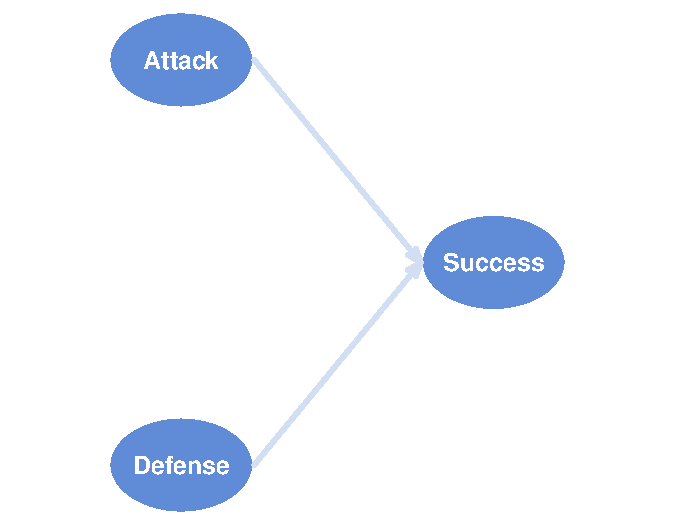
\includegraphics[width=.7\linewidth,height=.4\linewidth]{figure/plot_success_diagram} 

}

\caption[Diagram depicting our simple model]{Diagram depicting our simple model\label{fig:plot_success_diagram}}
\end{figure}


\end{knitrout}





\subsubsection*{Manifest Variables}
Although the essence of latent variables is that they cannot be directly measured, that does not mean they are nonsense or useless. To make them operative, latent variables are indirectly measured by means of variables which can be perfectly observed-measured. These types of variables are called \textbf{manifest variables} (MVs), also known as \textbf{indicators} or \textbf{items}. We assume that manifest variables contain information that reflect or indicate one aspect of the construct; hence we use the information contained in indicators to obtain an approximate representation of the latent variable.


\subsubsection*{Formative and Reflective Indicators}
Once we have assumed that latent variables can only be observed and measured indirectly through the use of manifest variables, we need to consider the ways in which latent variables are indirectly measured. Latent variables can be measured in two ways:
\begin{itemize}
 \item through their consequences or effects reflected on their indicators
 \item through different indicators that are assumed to cause the latent variables
\end{itemize}

In the first case, called \textit{reflective way}, manifest variables are considered as being caused by the latent variables. The second case is known as \textit{formative way} because the latent construct is supposed to be formed by its indicators. The main difference between the reflective and formative ways has to do with the causal-effect relationships between the indicators and the constructs (look at the direction of the arrows). The formative and reflective approaches for measuring a latent construct are illustrated in the next figure trough the Attack construct.




\begin{knitrout}
\definecolor{shadecolor}{rgb}{0.969, 0.969, 0.969}\color{fgcolor}\begin{figure}[h]


{\centering 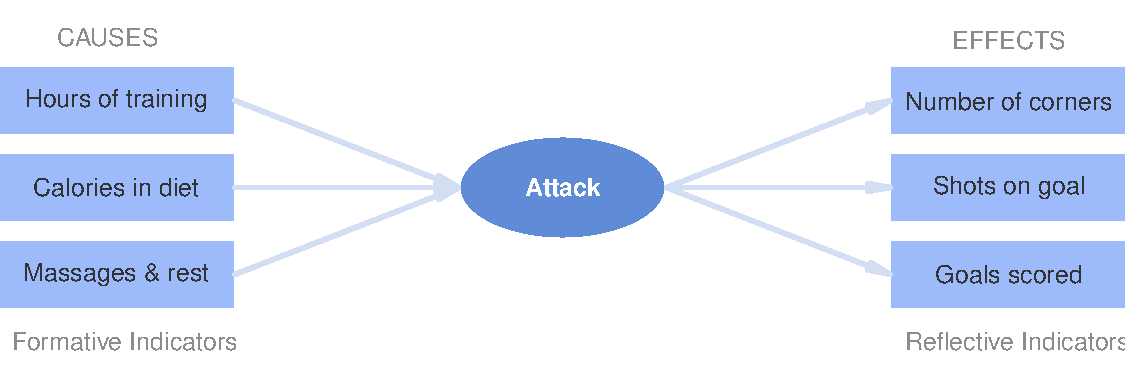
\includegraphics[width=.9\linewidth,height=.35\linewidth]{figure/measure_success_diagram} 

}

\caption[A latent variable measured by formative and reflective indicators]{A latent variable measured by formative and reflective indicators\label{fig:measure_success_diagram}}
\end{figure}


\end{knitrout}


Suppose that a researcher is studying a team trying to measure its quality of attack. She can use two approaches:
\begin{itemize}
 \item ask about different statistics \textbf{reflecting} the attack
 \item ask about possible practices \textbf{affecting} the attack 
\end{itemize}

Different effects might be evaluated, for example: the number of corner shots in every match, the number of shots on goal, or the number of goals scored. These are typical indicators of how good or bad the attack of a team is. The better the attack, the more number of any of these indicators. Conversely, the researcher might ask about the hours of training in the field, about the kind of food and the number of calories in the players diet, or the amount of time receiving massages and resting periods. The statistics about shots and goals can be considered as \textbf{reflective indicators} because they reflect the attack; patterns of training and care-taking practices can be seen as \textbf{formative indicators} because they are thought to contribute in the quality of attack. 


\subsection{Measuring Success, Attack and Defense}
We have proposed a model in which the Overall Success depends on the Quality of the Attack as well as on the Quality of the Defense. These are our three latent variables. Now we need to establish a set of indicators for each of the three constructs.

\paragraph{Block of Attack} If you check the available variables in the data \code{spainfoot}, you will see that the first four columns have to do with scored goals, which in turn can be considered to reflect the Attack of a team. We are going to take those variables as indicators of Attack:
\begin{itemize}
 \item GSH number of goals scores at home
 \item GSA number of goals scores away
 \item SSH percentage of matches with scores goals at home
 \item SSA percentage of matches with scores goals away
\end{itemize}

\paragraph{Block of Defense} The following four columns in the data (from 4 to 8) have to do with the Defense construct
\begin{itemize}
 \item GCH number of goals conceded at home
 \item GCA number of goals conceded away
 \item CSH percentage of matches with no conceded goals at home
 \item CSA percentage of matches with no conceded goals away
\end{itemize}

\paragraph{Block of Success} Finally, columns 9 to 12 can be grouped in a third block of variables, the block associated with Success
\begin{itemize}
 \item WMH number of won matches at home
 \item WMA number of won matches away
 \item LWR longest run of won matches
 \item LRWL longest run of matches without losing
\end{itemize}



\subsection{Path Model}
To be honest, our example is very simple because that's how textbook examples are. In this case, we don't require too much thought to decide what kind of measurement (reflective or formative) should be considered for the manifest variables. As you can tell, each block of variables reflects to some extent the latent construct they are associated with. Bear in mind that many times is not always clear whether an indicator should be treated as formative or reflective. In such cases we might need the assistant of an expert in the field we are working in to decide the type of measurement to be used.

We already saw a simple diagram with the relationships between the latent constructs. But now we need to take a step forward: we need to put all the pieces together and get the \textit{whole enchilada} diagram with both latent and manifest variables. To do this we use a \textbf{path diagram} or an arrow diagram. The function of these diagrams is to have a graphic representation of the relationships among all the variables present in our model. These types of diagrams can be drawn following a dozen of established rules and conventions. Through my experience, however, I've realized that I just need three of those principles for drawing my PLS path diagrams: 
\begin{enumerate}
 \item manifest variables are represented in a \textbf{rectangular} form
 \item latent variables are represented in an \textbf{elliptical} form
 \item relationships between variables are represented with \textbf{straight arrows}
\end{enumerate}
The graphical display of our complete model is as follows:




\begin{knitrout}
\definecolor{shadecolor}{rgb}{0.969, 0.969, 0.969}\color{fgcolor}\begin{figure}[h]


{\centering 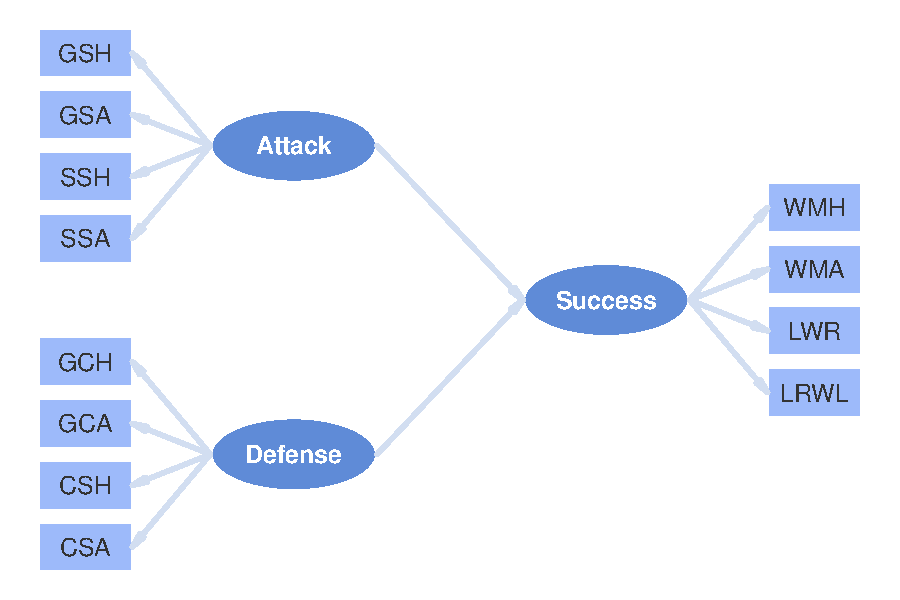
\includegraphics[width=.9\linewidth,height=.5\linewidth]{figure/spainfoot_model_diagram} 

}

\caption[Path Diagram depicting our simple model]{Path Diagram depicting our simple model\label{fig:spainfoot_model_diagram}}
\end{figure}


\end{knitrout}





\subsection{Inner and Outer models}
A full path model is comprised by two submodels: the structural model also known as \textbf{inner model} and the measurement model also known as \textbf{outer model}. The inner model is the part of the model that has to do with the relationships between latent variables. 
\begin{knitrout}
\definecolor{shadecolor}{rgb}{0.969, 0.969, 0.969}\color{fgcolor}\begin{figure}[h]


{\centering 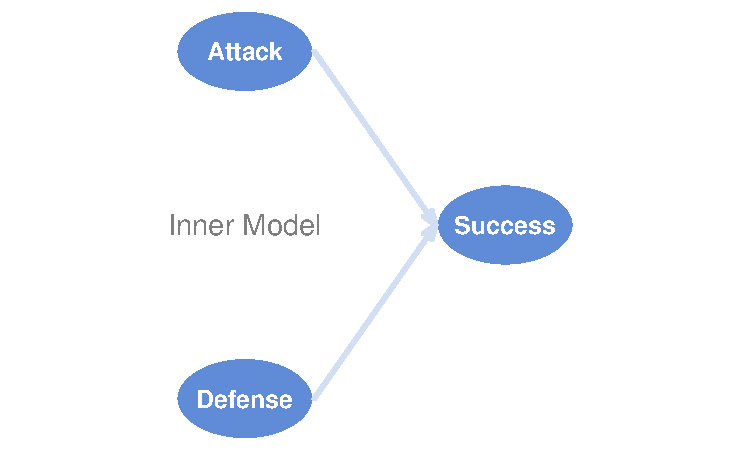
\includegraphics[width=.75\linewidth,height=.3\linewidth]{figure/spainfoot_inner_model_diag} 

}

\caption[Inner model]{Inner model: only relationships between latent variables\label{fig:spainfoot_inner_model_diag}}
\end{figure}


\end{knitrout}


The outer model is the part of the model that has to do with the relationships between each latent variable and its block of indicators
\begin{knitrout}
\definecolor{shadecolor}{rgb}{0.969, 0.969, 0.969}\color{fgcolor}\begin{figure}[h]


{\centering 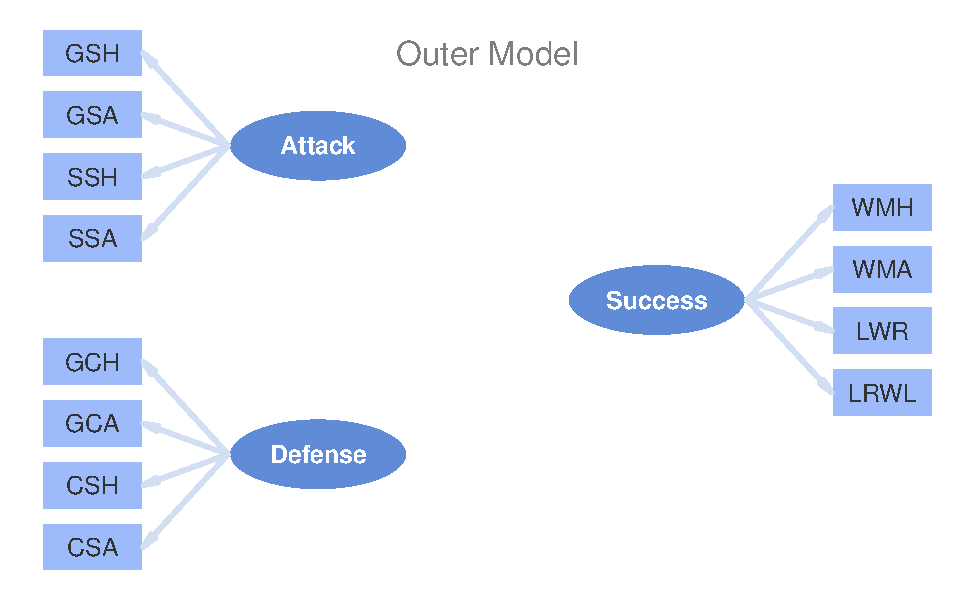
\includegraphics[width=.85\linewidth,height=.45\linewidth]{figure/spainfoot_outer_model_diag} 

}

\caption[Outer model]{Outer model: relationships between each construct and its indicators\label{fig:spainfoot_outer_model_diag}}
\end{figure}


\end{knitrout}




\section{Applying PLS-PM with the R package \plspm{}}
Finally we have our full structural model and its beautiful path diagram. Now what? What do we calculate in a PLS Path Model? Well, there are a lot things that can be (and that are actually) calculated in a PLS path model. But the most important ones, or at least the ones you have to remember, are the estimation of the latent variable scores and the quantification of the relationships in the model. For each arrow, we will obtain an associated numeric value representing the ``strength'' and ``direction'' of the relationship. For each latent construct, we will obtain a score. In some sense, we will get not only an \textit{Index of Success} but also an \textit{Index of Attack} and an \textit{Index of Defense}.


\subsection{Preparing the ingredients for \fplspm{}}
In order to perform a PLS-PM analysis the next step is to prepare the ingredients to start cooking our PLS path model with the function \fplspm{}. This function is pretty much the only function that you need to run the analysis. The tricky part, however, is to get the right ingredients in the right format to be plugged inside \fplspm{}. At least we need three mandatory ingredients: 1) a data set, 2) an inner model, and 3) an outer model. We already have the data in the data frame \code{spainfoot}. So let's talk about how to specify an inner model and an outer model for \fplspm{}.


\subsubsection*{Inner model matrix}
As we already mention, the inner or structural model represents the relationships between the latent variables. Looking at the diagram of the inner model, we can think of it as a flowchart representing a causal process. Moreover, we can think of the inner model as a network and by doing so we can represent it in matrix format. This is exactly what the second ingredient is for \fplspm{}: the \code{path\_matrix}. This is basically an R \code{matrix}, but not any kind of matrix. The \code{path\_matrix} must be a \textit{lower triangular boolean matrix}. In other words, it must be a square matrix (same number of rows and columns), the elements in the diagonal and above it must be zeros, and the elements below the diagonal can be either zeros or ones. Here's one way in which the inner matrix could be defined:
\begin{knitrout}
\definecolor{shadecolor}{rgb}{0.969, 0.969, 0.969}\color{fgcolor}\begin{kframe}
\begin{alltt}
\hlcomment{# rows of the inner model matrix}
Attack = \hlfunctioncall{c}(0, 0, 0)
Defense = \hlfunctioncall{c}(0, 0, 0)
Success = \hlfunctioncall{c}(1, 1, 0)

\hlcomment{# path matrix created by row binding}
foot_path = \hlfunctioncall{rbind}(Attack, Defense, Success)

\hlcomment{# add column names (optional)}
\hlfunctioncall{colnames}(foot_path) = \hlfunctioncall{rownames}(foot_path)
\end{alltt}
\end{kframe}
\end{knitrout}

What we are doing is creating three vectors that will be the rows of the argument \code{path\_matrix}. Then we use the function \code{rbind()} that creates a matrix by ``stacking'' the row vectors. And finally we use the row names of the matrix \code{foot\_path} as its column names. To see how the inner matrix looks like just type its name in the R console:

\begin{knitrout}
\definecolor{shadecolor}{rgb}{0.969, 0.969, 0.969}\color{fgcolor}\begin{kframe}
\begin{alltt}
\hlcomment{# let's see it}
foot_path
\end{alltt}
\begin{verbatim}
##         Attack Defense Success
## Attack       0       0       0
## Defense      0       0       0
## Success      1       1       0
\end{verbatim}
\end{kframe}
\end{knitrout}

The way in which you should read this matrix is by ``columns affecting rows''. A number one in the cell $i,j$ (i-th row and j-th column) means that column $j$ affects row $i$. For instance, the one in the cell 3,1 means that \texttt{Attack} affects \texttt{Success}. The zeros in the diagonal of the matrix mean that a latent variable cannot affect itself. The zeros above the diagonal imply that PLS-PM only works with recursive models (no loops in the inner model).

A nice feature available in \plspm{} is the function \code{innerplot()} that allows us to visualize the inner matrix in a path diagram format. This is specially useful when we want to visually inspect the model defined for \code{path\_matrix}.
\begin{knitrout}
\definecolor{shadecolor}{rgb}{0.969, 0.969, 0.969}\color{fgcolor}\begin{kframe}
\begin{alltt}
\hlcomment{# plot the path matrix}
\hlfunctioncall{innerplot}(foot_path)
\end{alltt}
\end{kframe}\begin{figure}[h]


{\centering 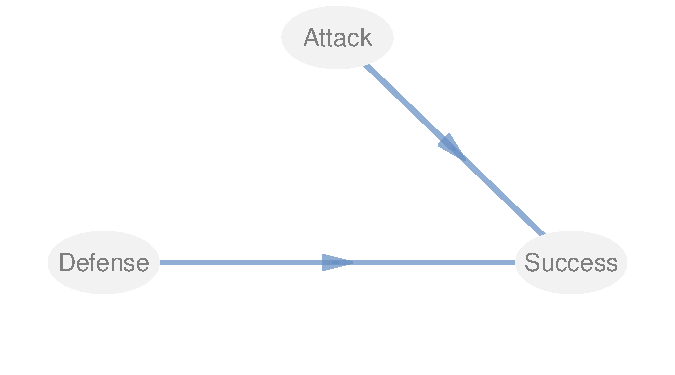
\includegraphics[width=.65\linewidth,height=.4\linewidth]{figure/innerplot_spainfoot} 

}

\caption[Visualizing the path diagram of the inner model with innerplot]{Visualizing the path diagram of the inner model with innerplot\label{fig:innerplot_spainfoot}}
\end{figure}


\end{knitrout}



\subsubsection*{Outer model list}
The third ingredient is the outer model. The way in which the outer model is defined is by using a \texttt{list} containing vectors. Basically, the idea is to indicate the set of manifest variables that form each block. In other words, we tell \fplspm{} what variables of the data are associated with what latent variables. The best thing is to explain this with an example.
\begin{knitrout}
\definecolor{shadecolor}{rgb}{0.969, 0.969, 0.969}\color{fgcolor}\begin{kframe}
\begin{alltt}
\hlcomment{# define list of indicators: what variables are associated with}
\hlcomment{# what latent variables}
foot_blocks = \hlfunctioncall{list}(1:4, 5:8, 9:12)
\end{alltt}
\end{kframe}
\end{knitrout}

The list above contains three elements, one per each block of indicators. Each element is a vector of indices. Thus, the first block corresponding to the latent variable \texttt{Attack} is associated with the first four columns of the data set. The second block, associated to \texttt{Defense}, is formed by columns from 5 to 8. And \texttt{Success} is associated with columns from 9 to 12. 


\subsubsection*{Vector of modes}
By default, \fplspm{} assumes that the measurement of the latent variables is in reflective mode, known as \textit{mode A} in the PLS-PM world. However, I strongly recommend you to explicitly define a vector of \code{modes}. This is indicated by using a character vector with as many letters as latent variables:
\begin{knitrout}
\definecolor{shadecolor}{rgb}{0.969, 0.969, 0.969}\color{fgcolor}\begin{kframe}
\begin{alltt}
\hlcomment{# all latent variables are measured in a reflective way}
foot_modes = \hlfunctioncall{c}(\hlstring{"A"}, \hlstring{"A"}, \hlstring{"A"})
\end{alltt}
\end{kframe}
\end{knitrout}

An alternative type of measurement is the formative mode, known as \textit{mode B}. So, if you had some latent variables in mode B, say \texttt{Success}, you would have to specify this as follows:
\begin{knitrout}
\definecolor{shadecolor}{rgb}{0.969, 0.969, 0.969}\color{fgcolor}\begin{kframe}
\begin{alltt}
\hlcomment{# Success in formative mode B}
foot_modes2 = \hlfunctioncall{c}(\hlstring{"A"}, \hlstring{"A"}, \hlstring{"B"})
\end{alltt}
\end{kframe}
\end{knitrout}



\subsection{Running \fplspm{}}
Now that we have all the necessary ingredients we are ready to run our first PLS path model with the all-mighty function \fplspm{}. The default usage of the function is: 

\code{plspm(Data, path\_matrix, blocks, modes = NULL)}

The function \fplspm{} has more parameters but right now we have sufficient with the \code{Data}, \code{path\_matrix}, \code{blocks} and \code{modes}. The first argument \code{Data} corresponds to the dataset \code{spainfoot}. The second parameter is the path matrix \code{foot\_path}. Then we have the list of blocks \code{foot\_blocks}, and finally the vector of modes \code{foot\_modes}. You have to respect the order in which the first three arguments are passed to \fplspm{}, otherwise you are going to get a nasty error message. Enter the following command to run the PLS-PM analysis:
\begin{knitrout}
\definecolor{shadecolor}{rgb}{0.969, 0.969, 0.969}\color{fgcolor}\begin{kframe}
\begin{alltt}
\hlcomment{# run plspm analysis}
foot_pls = \hlfunctioncall{plspm}(spainfoot, foot_path, foot_blocks, modes = foot_modes)
\end{alltt}
\end{kframe}
\end{knitrout}

Congratulations! You just run your first PLS Path Modeling analysis in R.

Here is how you would normally do all the previous steps in a single piece of code:
\begin{knitrout}
\definecolor{shadecolor}{rgb}{0.969, 0.969, 0.969}\color{fgcolor}\begin{kframe}
\begin{alltt}
\hlcomment{# rows of the path matrix}
Attack = \hlfunctioncall{c}(0, 0, 0)
Defense = \hlfunctioncall{c}(0, 0, 0)
Success = \hlfunctioncall{c}(1, 1, 0)

\hlcomment{# path matrix (inner model)}
foot_path = \hlfunctioncall{rbind}(Attack, Defense, Success)

\hlcomment{# add column names}
\hlfunctioncall{colnames}(foot_path) = \hlfunctioncall{rownames}(foot_path)

\hlcomment{# blocks of indicators (outer model)}
foot_blocks = \hlfunctioncall{list}(1:4, 5:8, 9:12)

\hlcomment{# vector of modes (reflective)}
foot_modes = \hlfunctioncall{c}(\hlstring{"A"}, \hlstring{"A"}, \hlstring{"A"})

\hlcomment{# run plspm analysis}
foot_pls = \hlfunctioncall{plspm}(spainfoot, foot_path, foot_blocks, modes = foot_modes)
\end{alltt}
\end{kframe}
\end{knitrout}


Initially, the definition of a pls path model for \fplspm{} might seem a little bit elaborate, especially for users accustomed to define their PLS path models using a graphic interface. Switching to \plspm{} may require thinking out of the box, but the invested effort has its dividends. One of the immediate rewards is that you stop wasting your time in mouse clicks and dragging objects to draw a path diagram. 


\subsubsection*{\fplspm{} output}
What we get in \code{foot\_pls} is an object of class \code{"plspm"}. Everytime you type an object of this class you will get a display with the following list of results:
\begin{knitrout}
\definecolor{shadecolor}{rgb}{0.969, 0.969, 0.969}\color{fgcolor}\begin{kframe}
\begin{alltt}
\hlcomment{# what's in foot_pls?}
foot_pls
\end{alltt}
\begin{verbatim}
## Partial Least Squares Path Modeling (PLS-PM) 
## ---------------------------------------------
##    NAME             DESCRIPTION
## 1  $outer_model     outer model
## 2  $inner_model     inner model
## 3  $path_coefs      path coefficients matrix
## 4  $scores          latent variable scores
## 5  $crossloadings   cross-loadings
## 6  $inner_summary   summary inner model
## 7  $effects         total effects
## 8  $unidim          unidimensionality
## 9  $gof             goodness-of-fit
## 10 $boot            bootstrap results
## 11 $data            data matrix
## ---------------------------------------------
## You can also use the function 'summary'
\end{verbatim}
\end{kframe}
\end{knitrout}


How do you know what class of object is \code{foot\_pls}? Use the function \code{class()} to get the answer:
\begin{knitrout}
\definecolor{shadecolor}{rgb}{0.969, 0.969, 0.969}\color{fgcolor}\begin{kframe}
\begin{alltt}
\hlcomment{# what class of object is foot_pls?}
\hlfunctioncall{class}(foot_pls)
\end{alltt}
\begin{verbatim}
## [1] "plspm"
\end{verbatim}
\end{kframe}
\end{knitrout}


If you want to inspect the matrix of path coefficients contained in \code{\$path\_coefs} simply type in your R console:
\begin{knitrout}
\definecolor{shadecolor}{rgb}{0.969, 0.969, 0.969}\color{fgcolor}\begin{kframe}
\begin{alltt}
\hlcomment{# path coefficients}
foot_pls$path_coefs
\end{alltt}
\begin{verbatim}
##         Attack Defense Success
## Attack  0.0000  0.0000       0
## Defense 0.0000  0.0000       0
## Success 0.7573 -0.2836       0
\end{verbatim}
\end{kframe}
\end{knitrout}


In the same manner, if you want to check the inner model results contained in \code{\$inner\_model}, just type:
\begin{knitrout}
\definecolor{shadecolor}{rgb}{0.969, 0.969, 0.969}\color{fgcolor}\begin{kframe}
\begin{alltt}
\hlcomment{# inner model}
foot_pls$inner_model
\end{alltt}
\begin{verbatim}
## $Success
##             Estimate Std. Error    t value  Pr(>|t|)
## Intercept -1.998e-16    0.09218 -2.167e-15 1.000e+00
## Attack     7.573e-01    0.10440  7.253e+00 1.349e-06
## Defense   -2.836e-01    0.10440 -2.717e+00 1.466e-02
\end{verbatim}
\end{kframe}
\end{knitrout}



In addition, there is a \code{summary()} method that you can apply to any obect of class \code{"plspm"}. This function gives a full summary with the standard results provided in most software for PLS Path Modeling. I won't display the bunch of stuff that \code{summary()} provides but I recommend you to check it out in your computer:
\begin{knitrout}
\definecolor{shadecolor}{rgb}{0.969, 0.969, 0.969}\color{fgcolor}\begin{kframe}
\begin{alltt}
\hlcomment{# summarized results}
\hlfunctioncall{summary}(foot_pls)
\end{alltt}
\end{kframe}
\end{knitrout}



\subsection{Plotting results}
With \plspm{} you can visualize some results using the function \code{plot()}. By default, this function displays the results of the inner model, that is, the path coefficients:
\begin{knitrout}
\definecolor{shadecolor}{rgb}{0.969, 0.969, 0.969}\color{fgcolor}\begin{kframe}
\begin{alltt}
\hlcomment{# plotting results (inner model)}
\hlfunctioncall{plot}(foot_pls)
\end{alltt}
\end{kframe}

{\centering 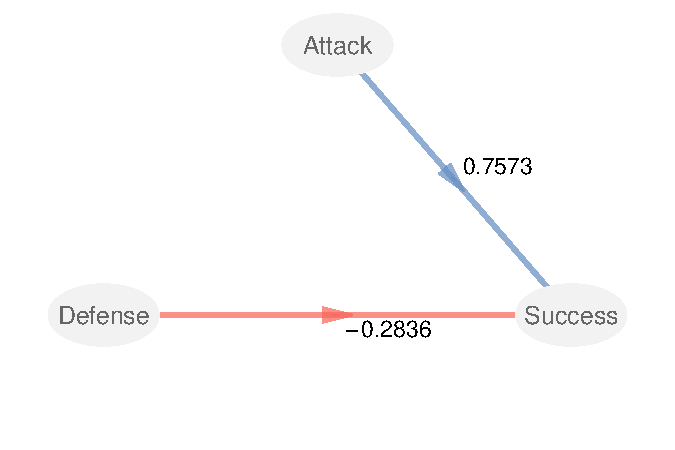
\includegraphics[width=.7\linewidth,height=.4\linewidth]{figure/plot_inner_foot_pls} 

}



\end{knitrout}


In order to check the results of the outer model, let's say the loadings, you need to use the parameter \code{what} (\code{what="loadings"}) of the \code{plot()} function:
\begin{knitrout}
\definecolor{shadecolor}{rgb}{0.969, 0.969, 0.969}\color{fgcolor}\begin{kframe}
\begin{alltt}
\hlcomment{# plotting loadings of the outer model}
\hlfunctioncall{plot}(foot_pls, what = \hlstring{"loadings"}, arr.width = 0.1)
\end{alltt}
\end{kframe}

{\centering 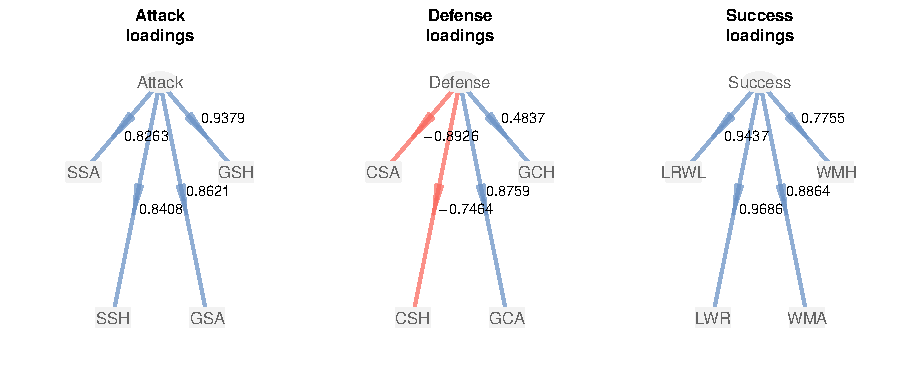
\includegraphics[width=1\linewidth,height=.45\linewidth]{figure/plot_loadings_foot_pls} 

}



\end{knitrout}



\subsubsection*{Show me the Index}
I promised you that we were going to get an \textit{Index of Success} for the teams in the Spanish football league. The way in which this is achieved in PLS Path Modeling is with the obtained latent variable scores contained in \code{\$scores}. Using the functions \code{head()} and \code{tail()} you can take a look at the first and last \code{n=5} rows, respectively:
\begin{knitrout}
\definecolor{shadecolor}{rgb}{0.969, 0.969, 0.969}\color{fgcolor}\begin{kframe}
\begin{alltt}
\hlcomment{# show me the first scores}
\hlfunctioncall{head}(foot_pls$scores, n = 5)
\end{alltt}
\begin{verbatim}
##             Attack  Defense Success
## Barcelona   2.6116 -1.74309  2.7891
## RealMadrid  1.7731 -1.13284  2.3246
## Sevilla    -0.1123 -2.24651  0.5541
## AtleMadrid  1.5334  0.02392  0.7771
## Villarreal  0.2801  0.16761  0.6084
\end{verbatim}
\begin{alltt}

\hlcomment{# show me the last scores}
\hlfunctioncall{tail}(foot_pls$scores, n = 5)
\end{alltt}
\begin{verbatim}
##             Attack Defense Success
## Valladolid -0.7615  0.4655 -0.7458
## Getafe      0.4188  0.6726 -0.9608
## Betis      -0.4853  0.5492 -0.5288
## Numancia   -1.4872  1.2356 -1.1348
## Recreativo -1.2255  0.7037 -0.9807
\end{verbatim}
\end{kframe}
\end{knitrout}


Before you draw any conclusions from the obtained results, we still need to do some adjustments to the model. After all, the negative path coefficient of \code{Defense} on \code{Success} does not correspond to one of the hypotheses stated in the theory: \textit{the better the quality of the Defense, the more Success}.

We need to make a stop before getting our hands full with all the stuff that is estimated in a PLS path model. I know we are just starting and we have yet to talk about all the provided results by \fplspm{} and how to interpret them. But let me end this chapter at this point while there is still (I hope so) some free space in your brain disk because in the next chapter we will discuss the bolts and nuts behind the PLS-PM methodology, and I guarantee you that is going to get a little bit dense.



\section{Reading List}
\begin{itemize}
 \item \textbf{\textsf{The Partial Least Squares Approach for Structural Equation Modeling}} by Wynne Chin. This chapter in the book \textit{Modern methods for business research} (edited by G. A. Marcoulides), provides an interesting review of the PLS approach from a SEM standpoint. Without heavy mathematical notation and targeted to a business and marketing audience, Chin explains PLS-PM in an approachable way for non-statisticians. Good reading for getting started with PLS-PM.
 \vspace{2mm}
 \item \textbf{\textsf{A Primer for Soft Modeling}} by R. Frank Falk and Nancy B. Miller (1992) Published by The University of Akron Press (Ohio), this is a short manuscript that aims to be an introductory level textbook for PLS Path Modeling.
\vspace{2mm}
 \item \textbf{\textsf{The Partial Least Squares (PLS) Approach to Causal Modelling: Personal Computer Adoption and Use as an Illustration}} by Barclay D., Higgins C. and Thompson R. (1995). This paper, in the Special Issue on Research Methodology of \textit{Technology Studies (Vol 2, Num 2: 285 - 309)}, describes an application of PLS-PM on Information Systems without using much mathematical notation. Good introduction if you are afraid of cryptic math equations.
\end{itemize}


% Chapter3

% !Rnw root = ../PLS_Path_Modeling_with_R.Rnw


\chapter{Setting the PLS-PM Framework}
This is the chapter where I get to wear the hat of the tedious statistician. As you know, every statistical method has an underlying theoretical background and a conceptual framework. That's where people list the assumptions and the conditions for the models, the data, and the proposed solutions. It is certainly not the most exciting part of the book but if I skip its contents all my mentors and colleagues will probably blame me for heresy. Not that I care a lot though, but I'm sure there would be some extremely dissapointed readers for not finding the information contained in this chapter. We'll begin with a short opinionated section that talks about the underlying \textit{frame of mind} in PLS Path Modeling. Next, we'll present the formal specifications of a PLS Path Model. And then we'll discuss how the algorithm works.



\section{PLS-PM Frame of Mind}
Before describing the PLS-PM methodology, I would like to tell you some words that you won't see that often in the PLS-related literature but that I consider very important to understand the PLS-PM framework. Although most of what is here is my personal point of view, I think it reflects enough what most \textit{PLSers} feel about the principles of PLS in general, and PLS-PM in particular.

First of all, you have to understand that PLS methods are analytical tools with algorithmic origins aiming at solving models in a very practical way. PLS methods are not derived through probabilistic reasoning or numerical optimization. Instead, PLS moves away from stringent assumptions on data while maintaining a prediction-oriented focus. It is true that it doesn't rely on the classic inferential tradition ---extensively based on assumptions about variables and error distributions--- but this does not mean that PLS lacks a solid statistical basis. To assess how closely a PLS model ``fits'' the data, we use prediction error as our measure of prediction accuracy, and resampling methods for inference purposes. 

From the Structural Equation Modeling (SEM) standpoint, PLS-PM offers a different approach that doesn't impose any distributional assumptions on the data that are hard to meet in real life, especially for non-experimental data. When we use a covariance-based SEM approach we are implicitly assuming that the data is generated by some ``true'' theoretical model. In this scenario, the goal of covariance structure analysis (CSA) is to recover the ``true'' model that gave rise to the observed covariances. Briefly, when using CSA we are concerned with fitting a model and reproducing the observed covariances. This approach resorts to classical theory of statistical inference and is based on a heavy use of distributional assumptions about the behavior and personality of the data. Consequently, the analyst is forced to move slowly; and the modeling process requires careful thought and stringent justifications that more often than not end up compromising the whole analysis with the bizarre (and sometimes contradictory) principle of \textit{the data must follow the model}. 

In contrast, PLS-PM does not rely on a data-generation process and causal-modeling interpretations. 
Instead, PLS-PM treats the data ``just'' as a dataset. What I mean by this is that although there can be a data-generation process in principle, it plays no direct role in PLS-PM. The proposed models are not considered to be ground truth, but only an approximation with useful predictiveness. In other words, PLS-PM assumes no model by which the data were generated. There is only the data and nothing but the data. In this sense, PLS-PM follows the spirit of a dimension reduction technique that we can use to get useful insight of the data on hand. The ultimate goal in PLS-PM is to provide a practical summary of how the set of dependent variables are systematically explained by their sets of predictors.

Besides the description of PLS Path Modeling as an alternative approach to SEM covariance structure analysis, PLS-PM can also be regarded as a technique for analyzing a system of relationships between multiple blocks of variables, or if you want to put it in simple terms, multiple data tables. There are many statistical methods that we can use to study data presented with several blocks of variables observed on the same subjects: Hort's Generalized Canonical Correlation Analysis, Carroll's Generalized Canonical Correlation analysis, Multiple Factor Analysis, etc. The idea behind all these methods is to identify or uncover a common structure among the blocks of variables.

From the Multiple Table Analysis standpoint, PLS-PM offers a great tool for analyzing high dimensional data in a low-structure environment. In particular, PLS-PM provides the nice feature of being used as a method for prediction purposes. Given the fact that a lot of mutiple table techniques are only focused on description and exploration tasks, PLS-PM can be used for more explanatory and confirmatory purposes.

In summary, we can regard PLS-PM as a coin with the two following faces:
\begin{itemize}
 \item PLS Path Modeling as a component-based alternative for estimating Structural Equation Models.
 \item PLS Path Modeling as a method for analyzing a system of linear relationships between multiple blocks of variables.
\end{itemize}


\section{PLS Path Modeling Specs}
Behind every statistical method there is a conceptual framework that we use to formally represent the ``stuff'' that we want to model, the way in which we want to model it, what do we want to obtain, and how can we obtain it. PLS-PM is no exception and we need to talk about the \textit{behind the scenes} of this methodology. I find it useful to distinguish between the \textbf{formal model} and the \textbf{operative model}. By \textit{formal model} I mean the statement of the theoretical model, the required assumptions, and the more or less abstract notions. By \textit{operative} I mean the computational side, that is, the proposed solution. In short: the formal model is ``what we want'' while the operative model is ``how to get what we want''.


\section{Formal Model: \textit{What we want}}
Let's start with the formalization of a PLS Path Model and its specifications. These are the things that live in the abstract universe of the statistical models. You can think of the specifications as our idealized representation of how the world looks like through the PLS-PM glass. Keep in mind, however, that this is just a representation of how the world ``could'' work, not how the world ``should'' work.

Every PLS Path Model is formed by two submodels: the structural or inner model, and the measurement or outer model. The structural model is the part of the model that has to do with the relationships between the latent variables. In turn, the measurement model is the part of the model that has to do with the relationships of a latent variable with its block of manifest variables.

\subsection*{Notation}
Let's assume that we have $p$ variables measured on $n$ observations (i.e. individuals, cases, samples), and that the variables can be divided in $J$ blocks. We will use the following notation in the rest of the chapter:
\begin{itemize}
 \item[] $\mathbf{X}$ is the data set containing the $n$ observations and $p$ variables. You can think of $\mathbf{X}$ as a matrix of dimension $n \mathsf{x} p$
 
 \item[] $\mathbf{X}$ can be divided in $J$ (mutually exclusive) blocks $\mathbf{X_1}, \mathbf{X_2}, \dots, \mathbf{X_J}$

 \item[] Each block $\mathbf{X_j}$ has $K$ variables: $X_{j1}, \dots, X_{jK}$
 
 \item[] Each block $\mathbf{X_j}$ is assumed to be associated with a latent variable $LV_j$. Keep in mind that $LV_j$ is just an abstract representation (i.e. unobserved).
 
 \item[] The estimation of a latent variable, also known as score, is denoted by $\widehat{LV_j} = Y_j$
\end{itemize}


\subsection{The Structural Model}
First, let us talk about the specifications of the structural part in a PLS Path Model. There are three things that you need to consider about the inner relationships:

\paragraph{1) Linear Relationships} The first aspect of an inner model is that we treat all the structural relationships as linear relationships. We can express the structural relations in mathematical notation as:
$$ LV_j = \beta_0 + \sum_{i \rightarrow j} \beta_{ji} LV_i + error_j$$
The subscript $i$ of $LV_i$ refers to all the latent variables that are supposed to predict $LV_j$. The coefficients $\beta_{ji}$ are the \textbf{path coefficients} and they represent the ``strength and direction'' of the relations between the response $LV_j$ and the predictors $LV_i$. $\beta_{0}$ is just the intercept term, and the $error_j$ term accounts for the residuals.

\paragraph{2) Recursive Models} The second thing you need to be aware of is that the system of equations must be a \textbf{recursive} system. What this means is that the paths formed by the arrows of the inner model cannot form a loop. 

\paragraph{3) Regression Specification} The third aspect about the inner relationships is something called \textit{predictor specification} which is just a fancy term to express a linear regression idea. That's why I prefer to call it \textit{regression specification}. The idea behind this specification is that the linear relationships are conceived from a standard regression perspective:

$$ E(LV_j | LV_i) = \beta_{0i} + \sum_{i \rightarrow j} \beta_{ji} LV_i $$

What we are saying in the previous equation, in a regression sense, is that we want to understand as far as possible the conditional expected values of the response $LV_j$ determined by its predictors $LV_i$. The only extra assumption is:

$$ cov(LV_j, error_j) = 0 $$

which means that a latent variable $LV_j$ is uncorrelated with the residual $error_j$. Notice that we are assuming nothing about the distributions of the variables and error terms. We are just requiring the existence of first and second order moments in the variables.



\subsection{The Measurement Model}
Now it's time to talk about the measurement or outer model. Remember this is the part of a model that has to do with the relationships between a latent variable and its block of manifest variables. The relevant aspect about the outer model that you should bare in mind is that there are two main measurement options: reflective blocks and formative blocks. 

\paragraph{1a) Reflective Way}
The most common type of measurement is the \textit{reflective} mode. In this case the latent variable is considered as the cause of the manifest variables. That's why it's called \textit{reflective} because the manifest variables are ``reflecting'' the latent variable. If we had a latent variable $LV_1$ measured with three indicators, we could represent them with the next path diagram (note the direction of the arrows):
\begin{knitrout}
\definecolor{shadecolor}{rgb}{0.969, 0.969, 0.969}\color{fgcolor}\begin{figure}[h]


{\centering 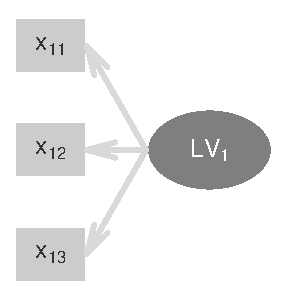
\includegraphics[width=.25\linewidth,height=.25\linewidth]{figure/reflective_way} 

}

\caption[Path diagram of a reflective block]{Path diagram of a reflective block\label{fig:reflective_way}}
\end{figure}


\end{knitrout}


\paragraph{1b) Formative Way}
The other type of measurement is the \textit{formative} mode. In this case the manifest variables are considered to be the cause of the latent variable. That's why it's called \textit{formative} because the manifest variables are ``forming'' the latent variable. If we had a latent variable $LV_2$ measured with three indicators, we could represent them with the next path diagram (note the direction of the arrows):
\begin{knitrout}
\definecolor{shadecolor}{rgb}{0.969, 0.969, 0.969}\color{fgcolor}\begin{figure}[h]


{\centering 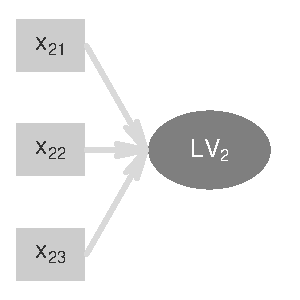
\includegraphics[width=.25\linewidth,height=.25\linewidth]{figure/formative_way} 

}

\caption[Path diagram of a formative block]{Path diagram of a formative block\label{fig:formative_way}}
\end{figure}


\end{knitrout}


\paragraph{2) Linear Relationships} Just like in the inner model, the outer model relationships are also considered to be linear. In mathematical notation, we have that:
$$ X_{jk} = \lambda_{0jk} + \lambda_{jk} LV_j + error_{jk}   \hspace{10mm}  \mathsf{Reflective}$$
$$ LV_j = \lambda_{0j} + \lambda_{jk} X_{jk} + error_j   \hspace{10mm}  \mathsf{Formative}$$
The coefficients $\lambda_{jk}$ are called \textbf{loadings}; $\lambda_{0}$ is just the intercept term, and the $error$ terms account for the residuals. Here I'm doing some notation abuse but it's to keep things simple.

\paragraph{3) Regression Specification} In addition, we also have the concept of \textit{predictor specification} or regression specification: the linear relationships are conceived from a standard regression perspective:

$$ E(X_{jk} | LV_j) = \lambda_{0jk} + \lambda_{jk} LV_j  \hspace{10mm}  \mathsf{Reflective} $$
$$ E(LV_j | X_{jk}) = \lambda_{0j} + \lambda_{jk} X_{jk}  \hspace{10mm}  \mathsf{Formative}$$

What we are saying in the previous equations in a regression sense is that we want to understand as far as possible the conditional expected values of the response variables (either manifest or latent) in terms of the predictor ones.


\subsection{The Weight Relations}
There's one last thing belonging to the specifications of a PLS Path Model that we need to mention: the \textit{weight relations}. So far we've talked about the theoretical specifications that give formal shape to the inner and the outer models. But there's one piece that is kind of in the air. Do you know what piece are we referring to? The latent variables! All the linear equations and the considered assumptions depend on the latent variables $LV_j$, but the issue is that they are virtual entities. I don't know if you remember what I said when I defined the notation but I clearly stated that: \textit{Keep in mind that $LV_j$ is just an abstract representation}. Maybe I wasn't clear enough but what I meant was that the latent variables $LV_j's$ are like ghost variables. Unless we have a way to materialize our abstract latent variables, all the previous specifications are worthless. But fear not. Thanks to the \textit{weight relations} we can bridge the gap between the virtual LVs and the material LVs. 

In PLS-PM, latent variables are estimated as a linear combination of their manifest variables. Moreover, an estimated $LV_j$ is called a \textbf{score}, which we'll denote as $Y_j$:
$$\widehat{LV_j} = Y_j = \sum_{k} w_{jk} X_{jk}$$
In fact, this is the very reason why PLS-PM is referred to as a \textit{component-based} approach because latent variables are calculated as a weighted sum of their indicators, something similar to what is done in principal component analysis.

It is important not to confuse the role that plays the abstract $LV_j$ with the role that plays the score $Y_j$. Yes, they both refer to the same construct, but while the former is used for theoretical reasons, the later is used for practical purposes. I know this can muddle you up but don't worry.  It doesn't matter if a latent variable is measured in a reflective or a formative way; a latent variable is calculated as a linear combination of its block of indicators.




\section{Operative Model: \textit{How to get what we want}}
So far we've been discussing the specifications behind any PLS Path Model. Remember that these specifications are an idealized representation of the world looked at through the PLS-PM glass. In sum, we've only talked about ``what we want''; now we need to discuss the operative side which is basically: ``how to get what we want''.

The basic idea of PLS Path Modeling is to combine the manifest variables of each block to form an estimated (proxy) latent variable. Once the latent scores are calculated, we proceed with the estimation of the path coefficients and the loadings. That's the overall route to follow. What we need is to define the way in which we are going to calculate things (the scores, the path coefficients, and the loadings). 


\subsubsection*{PLS-PM Algorithm Overview}
PLS Path Modeling follows a sequential procedure that can be divided in three major stages:
\begin{itemize}
 \item[] Stage 1: Get the weights to compute latent variable scores
 \item[] Stage 2: Estimating the path coefficients (inner model)
 \item[] Stage 3: Obtaining the loadings (outer model)
\end{itemize}

\vspace{2mm}
The first stage consists of obtaining the weights that will be used to get the scores of the latent varibles. The second stage has to do with estimating the path coefficients of the inner model. And the third stage involves the computation of the loadings (outer model). 

Of all the stages, the first one is the key part of the PLS-PM methodology. By the way, this is also the tricky part. This stage is an iterative process in which the ultimate goal is to get the weights for the famous \textit{weight relations}. This is the heart of the PLS-PM methodology and it allows us to materialize the ghostly-abstract latent variables. Once we pass the first stage, the next two stages are practically a piece of cake. The estimation of the path coefficients is just a matter of running as many least squares regressions as structural equations in the model. In turn, obtaining the loadings is just a matter of computing simple correlations. 

In its purest essence, the PLS-PM algorithm is nothing more than a series of simple and multiple ordinary least squares regressions. The slippery part comes with the multiple options for deciding what kind of regression to apply, and some extra input settings we need to consider. From my personal experience, this part is perhaps the main source of confusion and intimidation for most beginners. 


\subsection*{Auxiliary Model}
For convenience, let's use a simple model to make things a little less abstract. The complete model is illustrated in the following diagram:




\begin{knitrout}
\definecolor{shadecolor}{rgb}{0.969, 0.969, 0.969}\color{fgcolor}\begin{figure}[h]


{\centering 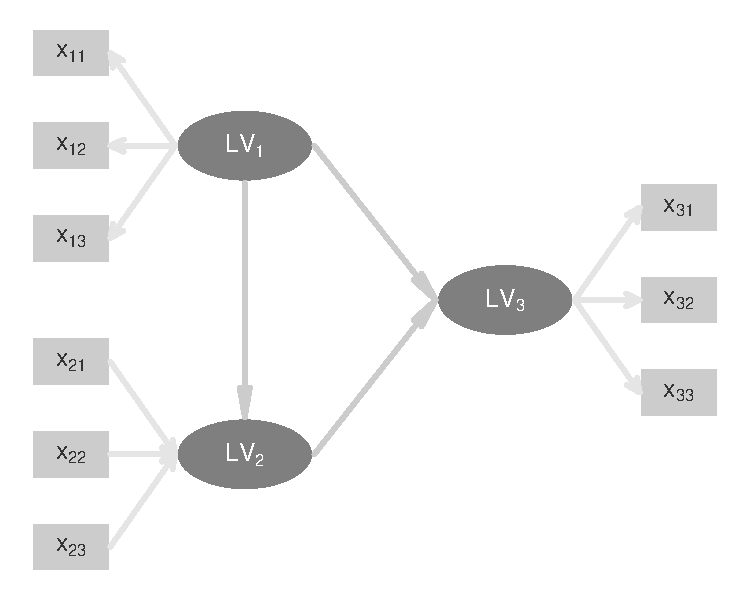
\includegraphics[width=.7\linewidth,height=.5\linewidth]{figure/auxiliary_path_diagram} 

}

\caption[Diagram of our auxiliary model]{Diagram of our auxiliary model\label{fig:auxiliary_path_diagram}}
\end{figure}


\end{knitrout}



We are going to use a model with three latent variables: $LV_1$, $LV_2$, and $LV_3$. Each latent variable is associated with three manifest variables in the following form: $LV_1$ and $LV_3$ are reflective blocks:
$$ X_{1k} = \lambda_{1k} LV_1 + error \hspace{5mm} k = 1, 2, 3$$
$$ X_{3k} = \lambda_{3k} LV_3 + error \hspace{5mm} k = 1, 2, 3$$

In turn, $LV_2$ is a formative block:
$$ LV_2 = \sum_{k} \lambda_{jk} X_{2k} + error  \hspace{5mm} k = 1, 2, 3$$

For the structural relationships we are going to suppose two equations. One inner relationship in which $LV_2$ depends on $LV_1$:
$$ LV_2 = \beta_{21} LV_1 + error $$

The other inner relationship in which $LV_3$ depends on $LV_1$ and $LV_2$:
$$ LV_3 = \beta_{31} LV_1 + \beta_{32} LV_2 + error $$

Additionally, we will assume that all the variables are standardized (mean=0, var=1), in this way we get rid of the annoying constant terms $\beta_{0}'s$ and $\lambda_{0}'s$. 


\subsection{Stage 1: Iterative Process}
The first stage of the PLS-PM algorithm involves the computation of the weights to get the scores of the latent variables. Please keep in mind that our final PLS-PM destination is to get estimates of both the latent variables and the parameters (coefficients and loadings). The iterative procedure of the PLS algorithm, using technical jargon, proceeds as follows:
\vspace{2mm}
\begin{itemize}
 \item Start: Initial arbitrary outer weights (normalized to obtain standardized LVs)
 \item Step 1: Compute the external approximation of latent variables
 \item Step 2: Obtain inner weights
 \item Step 3: Compute the internal approximation of latent variables
 \item Step 4: Calculate new outer weights
 \item[] Repeat step 1 to step 4 until convergence of outer weights
\end{itemize}
\vspace{2mm}

If you are not familiar with the PLS argot, I bet you understand almost nothing from the previous pseudo-code of the iterative stage. There's a bunch of fanciful terminology such as \textit{outer weights}, \textit{normalized}, \textit{standardized}, \textit{external approximation}, \textit{inner weights}, and \textit{internal approximation}. I know all these terms may not make too much sense to you right now but you'll get them in the next pages (or so I hope).

First of all: if there's something that you need to have room in your head for is that a latent variable is calculated as a weighted sum of its manifest variables. This is the overriding principle that you should always remember. Repeat after me: \textit{latent variable scores are calculated as weighted sums of their indicators}. Good. In mathematical notation the previous sentence is expressed as:
$$\widehat{LV_j} = Y_j = \sum_{k} w_{jk} X_{jk}$$

The weights $w_{jk}$ to form the weighted average $\sum_{k} w_{jk} X_{jk}$ receive the especial name of \textit{outer weights}. Why \textit{outer}? Because there is another type of weights, called the \textit{inner weights}, that also appear in the iterative procedure. We'll talk about them in a second. The other thing that you need to know is that anything that has to do with the outer (measurement) model is referred to as \textit{external} or \textit{outside}. Likewise, anything that has to do with the inner (structural) model is referred to as \textit{internal} or \textit{inside}.


\subsubsection*{Step 0: Initial arbitrary outer weights}
We start the iterative process by assigning ``arbitrary'' values to the outer weights. To keep things simple, we can initialize all weights equal to one: $\tilde{w}_{jk}=1$. Taking our auxiliary model into account this implies creating three vectors $\mathbf{\tilde{w}}_k$ with all components equal to 1:
$$ \mathbf{\tilde{w}}_1 = (\tilde{w}_{11}=1, \tilde{w}_{12}=1, \tilde{w}_{13}=1) $$
$$ \mathbf{\tilde{w}}_2 = (\tilde{w}_{21}=1, \tilde{w}_{22}=1, \tilde{w}_{23}=1) $$
$$ \mathbf{\tilde{w}}_3 = (\tilde{w}_{31}=1, \tilde{w}_{32}=1, \tilde{w}_{33}=1) $$
Actually, the tilde weights $\tilde{w}_{jk}$ are not exactly the outer weights. We need to apply a little transformation that involves normalizing them so that the resulting scores have unit variance.

\subsubsection*{Step 1: External estimation}
Once we have the tilde weights $\mathbf{\tilde{w}}_k$, we get the \textit{external estimation} which consists of expressing a latent variable as a weighted sum of its indicators. In matrix notation we have
$$ Y_k \propto \mathbf{X}_k \mathbf{\tilde{w}}_k   \hspace{5mm}   k = 1, 2, 3  $$ 
Decomposing the formula for each LV we get the following:
$$ Y_1 \propto 1 X_{11} + 1 X_{12} + 1 X_{13} $$
$$ Y_2 \propto 1 X_{21} + 1 X_{22} + 1 X_{23} $$
$$ Y_3 \propto 1 X_{31} + 1 X_{32} + 1 X_{33} $$

As you can tell, I'm using the proportional symbol $\propto$ to indicate that each score $Y_j$ depends on its manifest variables $X_{jk}$ although there's something missing. To be precise with the formula of the scores we need to use the following equation:
$$ Y_j = \pm f_j \sum_{k} \tilde{w}_{jk} X_{jk} $$

Ok, now it seems that everything is getting fuzzy. Why is there a sign $\pm$ and what is $f_j$? The symbol $\pm$ is there to represent a weird phenomenon that may occur when calculating scores: the mysterious \textit{sign ambiguity}. The term $f_j$ is simply a scalar (a number) that makes $Y_j$ to be standardized. The phenomenon of the \textit{sign ambiguity} has to do when not all the indicators of a construct share the same correlation sign. It could be the case that instead of having all indicators positively correlated among them, there might be at least one of them that is negatively correlated. So to avoid problems deciding whether to use a positive or negative sign, we use a democratic approach to solve the \textit{sign ambiguity}. The solution is very simple: choose the sign so that the majority of the $X_{jk}$ is positively correlated with $Y_j$
$$sign\left[  \sum_{k} sign\left\{cor(X_{jk}, Y_j)\right\} \right]$$

The standardized LVs are finally expressed as:
$$ Y_j = \sum_{k} w_{jk} X_{jk} $$
where the weights $w_{jk}$ are the ``definite'' outer weights. In our example we have:
$$ Y_1 = w_{11} X_{11} + w_{12} X_{12} + w_{13} X_{13} $$
$$ Y_2 = w_{21} X_{21} + w_{22} X_{22} + w_{23} X_{23} $$
$$ Y_3 = w_{31} X_{31} + w_{32} X_{32} + w_{33} X_{33} $$


\subsubsection*{Step 2: Obtain Inner weights}
Once we have the initial scores of the latent variables, we put our focus on the inner model. Remember that the inner model takes into account only the relationships between latent variables. The goal in this step is to re-calculate scores but this time in a different way. Instead of getting the score of a latent varibale as a linear combination of its indicators, we will get a score as the linear combination of its associated latent variables. In other words, the connections among constructs in the inner model are taken into account in order to obtain a proxy of each latent variable calculated this time as a weighted aggregate of its adjacent LVs. The internal estimation of $LV_j$ denoted by $Z_j$ is defined by:
$$ Z_j = \sum_{i \longleftrightarrow j} e_{ij} Y_i $$
The double-headed arrow $\longleftrightarrow$ means that $LV_j$ is associated or connected with $LV_i$. If there is an arrow between $LV_j$ and $LV_i$ (it doesn't matter which is the dependent and which one the independent), then $LV_i$ must be taken into consideration for calculating $Z_j$. Because now we are dealing with the inner model, the weights $e_{ij}$ for this special combination are called \textit{inner weights}. 

The seemingly complication for PLS \textit{rookies} comes with the various options or \textit{schemes} that we have to obtain the inner weights  $e_{ij}$. There are three options to calculate the inner weights:
\begin{itemize}
 \item Centroid scheme
 \item Factor scheme
 \item Path scheme
\end{itemize}

\paragraph{Centroid scheme} This scheme only considers the sign direction of the correlations between an LV and its adjacent (neighboring) LVs. The inner weights are defined as:
$$ e_{ji} = \left\{ \begin{array}{rc}
  sign \left[ cor(Y_j, Y_i)\right] & LV_j, LV_i \hspace{2mm} adjacents \\
  0 & otherwise
  \end{array} \right\}
$$
This option does not consider the direction nor the strength of the paths in the structural model. So in theory, some problems may be present when a correlation is close to zero, causing a sign changing from +1 to -1 during the iterations.

\paragraph{Factor scheme} This scheme uses the correlation coefficient as the inner weight instead of using only the sign of the correlation. The inner weights are defined as:
$$ e_{ji} = \left\{ \begin{array}{rc}
  cor(Y_j, Y_i) & LV_j, LV_i \hspace{2mm} adjacents \\
  0 & otherwise
  \end{array} \right\}
$$
This scheme considers not only the sign direction but also the strength of the paths in the structural model.

\paragraph{Path scheme} In this case the LVs are divided in antecedents (predictors) and followers (predictands) depending on the cause-effects relationships between two LVs. An LV can be either a follower, if it is caused by another LV, or an antecedent if it is the cause of another LV. If $LV_i$ is a follower of $LV_j$ then the inner weight is equal to the correlation between $Y_i$ and $Y_j$. On the other hand, for the antecedents $LV_i$ of $LV_j$ the inner weights are the regression coefficient of $Y_i$ in the multiple regression of $LV_j$ on the $LV_i's$ associated to the antecedents of $LV_j$.
The path weighting scheme has the advantage of taking into account both the strength and the direction of the paths in the structural model. However, this scheme presents some problems when the LV correlation matrix is singular.

\vspace{2mm}
In practice, choosing one weighting scheme in particular over the others has little relevance on the estimation process. It has been observed that they do not influence the results significantly. However, in a more theoretical level, they are of a great importance to understand how PLS-PM can be applied to different techniques of multiple table analysis.


\subsubsection*{Step 3: Internal Approximation}
One we have the inner weights, we compute the internal estimation $Z_j$ as:
$$ Z_j = \sum_{i \longleftrightarrow j} e_{ij} Y_i $$

In our auxiliary example we would have:
$$ Z_1 = \sum_{i \longleftrightarrow 1} e_{i1} Y_i = e_{21} Y_2 + e_{31} Y_3 $$
$$ Z_2 = \sum_{i \longleftrightarrow 2} e_{i2} Y_i = e_{12} Y_1 + e_{32} Y_3 $$
$$ Z_3 = \sum_{i \longleftrightarrow 3} e_{i3} Y_i = e_{13} Y_1 + e_{23} Y_2 $$



\subsubsection*{Step 4: Updating Outer weights}
Once the inside approximation is done, the internal estimates $Z_j$ must then be considered with regard their indicators. This is done by updating the outer weights. There are basically two ways of calculating the outer weights $w_{ji}$: (1) mode A, and (2) mode B. Each mode corresponds to a different way of relating the MVs with the LVs in the theoretical model. Mode A is used when the indicators are related to their latent variable through a reflective way. Instead, mode B is preferred when indicators are associated with their latent variable in a formative way

\paragraph{Mode A} In reflective blocks (mode A) we obtain the outer weights $\tilde{w}_{jk}$ with simple regressions of each indicator $X_{j1}, X_{j2}, \dots, X_{jk}$ on their latent score $Y_j$
$$ \tilde{w}_{jk}= (Y'_j Y_j)^{-1} Y'_j X_{jk} $$

\paragraph{Mode B} In formative blocks (mode B) we obtain the vector of outer weights $\mathbf{\tilde{w}_j} $ with a multiple regression of $Y_j$ on $\mathbf{X}_j$
$$ \mathbf{\tilde{w}_j} = (\mathbf{X}'_j \mathbf{X}_j)^{-1} \mathbf{X}'_j Y_j $$


\subsubsection*{Check for convergence}
In every iteration step, say $S = 1, 2, 3, \dots, $ convergence is checked comparing the outer weights of step $S$ against the outer weights of step $S-1$. One common way to check convergence is
$|w_{jk}^{S-1} - w_{jk}^{S}| < 10^{-5}$
as a convergence criterion.



\subsection{Stage 2: Path Coefficients}
The second stage of the algorithm consists of calculating the path coefficient estimates, $\widehat{\beta_{ji}} = B_{ji}$. The structural coefficients are estimated by ordinary least squares in the multiple regression of $Y_j$ on the $Y_i$'s related with it: 
$$ Y_j = \sum_{i \longrightarrow j} \widehat{\beta_{ji}} Y_i $$
The least squares solution is:
$$ B_{ji} = (Y_i' Y_i)^{-1} Y_i' Y_j $$


\subsection{Stage 3: Loadings}
The third stage of the algorithm consists of calculating the loadings. For convenience and simplicity reasons, loadings are preferably calculated as correlations between a latent variable and its indicators
$$ \widehat{\lambda_{jk}} = cor(X_{jk}, Y_j) $$



\subsection{Wrapping up}
The goal of PLS is to obtain score values of latent variables for prediction purposes. The idea is to calculate estimates of latent variables as linear combinations of their associated indicators using a special linear combination. We look for a linear combination in such a way that the obtained latent variables take into account the relationships of the structural and the measurement models in order to maximize the explained variance of the dependent variables (both latent and observed variables). 

The core of the PLS algorithm is the calculation of the weights (for the linear combination) required to estimate the latent variables. The weights are obtained based on how the structural and the measurement model are specified. This is done by means of an iterative procedure in which two kinds of approximation for the latent variables are alternated until convergence of weight estimates. These two types of approximation, called the inside approximation and the outside approximation, have to do with the inner relations and the outer relations, respectively.

The algorithm begins with arbitrary initial weights used to calculate an outside approximation of the latent variables, that is, initial weights are given in order to approximate the LVs as linear combinations of their MVs. Then, the inner relations among LVs are considered in order to calculate the inside approximations, having the option of choosing between three possible scenarios, called weighting schemes, to perform this approximation: (1) centroid, (2) factor, and (3) path scheme. Once the inside approximations are obtained, the algorithm turns around to the outer relations when new weights are calculated considering how the indicators are related to their constructs: by mode A (reflective), or by mode B (formative). Mode A implies simple linear regressions while mode B implies multiple linear regressions. The simple and/or multiple regressions coefficients are then used as new weights for an outside approximation. The process continues iteratively until convergence of the weights is reached.

After convergence of the outer weights, and once the latent variables are estimated, the parameters of the structural and the measurement models can be obtained. The path coefficients are calculated by ordinary least squares regressions between LVs. There are as many regressions as endogenous latent variables. The loading coefficients, are also estimated by least squares regressions but taking into account the kind of mode to be used (reflective or formative).




\section{Reading List}
\begin{itemize}
 \vspace{2mm}
 \item \textbf{\textsf{PLS path modeling}} by Michel Tenenhaus, Vincenzo Esposito Vinzi, Yves-Marie Chatelin, and Carlo Lauro (2005). This paper in the journal \textit{Computational Statistics \& Data Analysis (48: 159-205)} is perhaps the mandatory reference for anyone interested in the specifications and computational aspects of PLS-PM with a recent publication.
 
\vspace{2mm}
 \item \textbf{\textsf{Partial least squares}} by Herman Wold (1985). This entry in the \textit{Encyclopedia of Statistical Sciences, Vol 6: 581-591} is one of the classic PLS-PM references for anyone who wants to check pne of the original sources of Herman Wold.

 \vspace{2mm}
 \item \textbf{\textsf{Systems under indirect observation: causality, structure, prediction. Vol II}} edited by Karl Joreskog and Herman Wold (1982). The first chapter by Herman Wold is also another classic reference dedicated to explain the \textit{Soft Modeling} methodology of PLS-PM.

 \vspace{2mm}
 \item \textbf{\textsf{Model Construction and Evaluation When Theoretical Knowledge is Scarce: Theory and Application of Partial Least Squares}} by Herman Wold (1980). This paper, in the book \textit{Evaluation of Econometric Models} (edited by Kmenta and Ramsey, pp: 47-74), is not very cited but is worth reading in order to understand Wold's perspective on model building, as well as the basic principles behind PLS Path Modeling. \\
 Available at: \\
 \texttt{\href{http://www.nber.org/chapters/c11693}{http://www.nber.org/chapters/c11693}}

 \vspace{2mm}
 \item \textbf{\textsf{Latent Variables Path Modeling with Partial Least Squares}} by Jan-Bernd Lohmoller (1989). This purple-cover book is another official reference for PLS-PM, although this is definitely not a text for people with phobia to heavy math notation. The best thing about this book is that it presents a detailed and wide-ranging account of the capabilities of PLS-PM. It covers all the statistical, modeling, algorithmic and programming aspects of the PLS methodology. The worst thing: is not user (reader)-friendly. Written in his very particular \textit{Lohmollerian} style, it can be extremely hard to decipher. It took me several readings to start grasping the notions and connecting the dots. Not an easy going text but worth it if you are planning to open new paths in the PLS field. 
 
\end{itemize}


% Chapter4

% !Rnw root = ../PLS_Path_Modeling_with_R.Rnw


\chapter{Interpreting PLS-PM Results}
In chapter 2 we saw a basic PLS Path Modeling application using \plspm{} with the \textit{Spanish Football Success Index}. As you will recall, our model is based on a very simple theory:
\begin{quotation} \noindent
\textit{the better the quality of the \textbf{Attack}, as well as the quality of the \textbf{Defense}, the more \textbf{Success}.}
\end{quotation}





\begin{knitrout}
\definecolor{shadecolor}{rgb}{0.969, 0.969, 0.969}\color{fgcolor}\begin{figure}[h]


{\centering 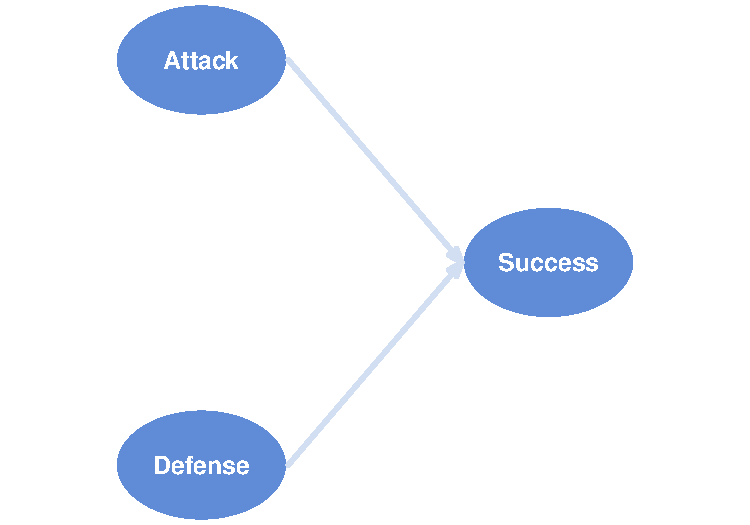
\includegraphics[width=.7\linewidth,height=.4\linewidth]{figure/success_inner_model_reminder} 

}

\caption[Diagram depicting the structural part of the Success model]{Diagram depicting the structural part of the Success model\label{fig:success_inner_model_reminder}}
\end{figure}


\end{knitrout}



Defining a PLS path model and applying the function \fplspm{} are just the first steps of a PLS Path Modeling analysis. The next thing to do is even more important: examining the obtained results and evaluating the quality of the model. In this chapter we are going to review some general guidelines for applying PLS-PM, and we will discuss the bells and whistles of how to interpret the output and diagnose the results.



\section{Reminder of Our Success Index Model}
As mentioned in the last two chapters, a PLS path model is comprised by two submodels: the structural model also known as \textbf{inner model} and the measurement model also known as \textbf{outer model}. The inner model is the part of the model that has to do with the relationships between latent variables. The outer model is the part of the model that has to do with the relationships between each latent variable and its block of indicators. The graphical display of the complete Success Model is shown in the next diagram:
\begin{knitrout}
\definecolor{shadecolor}{rgb}{0.969, 0.969, 0.969}\color{fgcolor}\begin{figure}[h]


{\centering 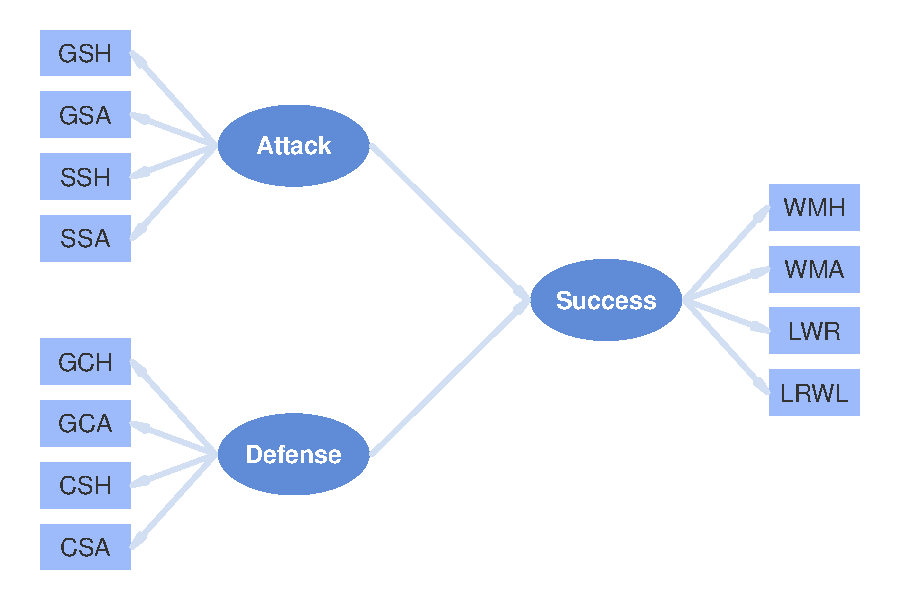
\includegraphics[width=.85\linewidth,height=.5\linewidth]{figure/success_path_diagram_reminder} 

}

\caption[Path Diagram depicting our simple model]{Path Diagram depicting our simple model\label{fig:success_path_diagram_reminder}}
\end{figure}


\end{knitrout}




\subsection{PLS-PM with \plspm{}}
I'm assuming that you already installed the package \plspm{} as described in Chapter 1. The data for our model comes with \plspm{} under the name \texttt{spainfoot}. Remember that you need to use the function \code{library()} to load the package in your current R session. To get access to the data, simply load it with the function \code{data()}:



\begin{knitrout}
\definecolor{shadecolor}{rgb}{0.969, 0.969, 0.969}\color{fgcolor}\begin{kframe}
\begin{alltt}
\hlcomment{# load package plspm}
\hlfunctioncall{library}(plspm)

\hlcomment{# load data spainfoot}
\hlfunctioncall{data}(spainfoot)
\end{alltt}
\end{kframe}
\end{knitrout}



\subsection{The function \fplspm{}}
The main function of the \plspm{} package is the function with the same name \fplspm{}. This function has 12 arguments that can be broken down in three main sets according to their purpose. The first set has to do with the parameters that you use to define a PLS Path Model. The second set of parameters are related with the PLS algorithm. The last group of parameters are additional options like validation and recovering the data matrix used in the computations:

\begin{itemize}
 \item \textbf{Parameters to define the PLS Path Model}
  \begin{itemize}
   \item[] \code{Data} (where you have the data)
   \item[] \code{path\_matrix} (defines the inner model)
   \item[] \code{blocks} (list defining the blocks of variables of the outer model)
   \item[] \code{scaling} (list defining the measurement scale of variables for non-metric data)
   \item[] \code{modes} (vector defining the measurement mode of each block)
  \end{itemize}

 \item \textbf{Parameters related to the PLS-PM algorithm}
  \begin{itemize}
   \item[] \code{scheme} (inner path weighting scheme)
   \item[] \code{scaled} (indicates whether the data should be standardized)
   \item[] \code{tol} (tolerance threshold for checking convergence of the iterative stage in the PLS algorithm)
   \item[] \code{maxiter} (maximum number of iterations)
   \item[] \code{plscomp} (indicates the number of PLS components ---per block--- when handling non-metric data)
  \end{itemize}

 \item \textbf{Additional parameters}
  \begin{itemize}
   \item[] \code{boot.val} (indicates whether bootstrap validation must be performed)
   \item[] \code{br} (number of bootstrap resamples)
   \item[] \code{plsr} (indicates whether path coefficients should be calculated by pls regression)
   \item[] \code{dataset} (indicates whether the data matrix should be retrieved)
  \end{itemize}
\end{itemize}
 
\vspace{2mm}
Even though there are 14 parameters to play with, most of the times you would probably need to tweak just a few of them. In fact, the most important ingredients are the first three arguments: \code{Data}, \code{path\_matrix}, and \code{blocks}. These ingredients don't have default settings so you must provide values for each of them. The rest of parameters come with predefined values which you can change depending on your needs and preferences. To see the specific details of each parameter you can consult the technical documentation with the function \code{help()}
\begin{knitrout}
\definecolor{shadecolor}{rgb}{0.969, 0.969, 0.969}\color{fgcolor}\begin{kframe}
\begin{alltt}
\hlcomment{# information about the function plspm()}
\hlfunctioncall{help}(plspm)
\end{alltt}
\end{kframe}
\end{knitrout}




\subsubsection*{Preparing the ingredients for \fplspm{}}
A PLS path model has to be specified with the mqndqtory arguments \code{Data}, \code{path\_matrix}, and \code{blocks}. In addition, it is recomended to specify the argument \code{modes} as well. Just like we did in chapter 2, here's how the ingredients for \fplspm{} can be prepared to cook our PLS path model:

\paragraph{Inner Matrix:} 
This is the inner model defined in matrix format
\begin{knitrout}
\definecolor{shadecolor}{rgb}{0.969, 0.969, 0.969}\color{fgcolor}\begin{kframe}
\begin{alltt}
\hlcomment{# rows of the path matrix}
Attack = \hlfunctioncall{c}(0, 0, 0)
Defense = \hlfunctioncall{c}(0, 0, 0)
Success = \hlfunctioncall{c}(1, 1, 0)

\hlcomment{# creating the matrix by binding rows}
foot_path = \hlfunctioncall{rbind}(Attack, Defense, Success)

\hlcomment{# add column names (optional)}
\hlfunctioncall{colnames}(foot_path) = \hlfunctioncall{rownames}(foot_path)

\hlcomment{# let's see it}
foot_path
\end{alltt}
\begin{verbatim}
##         Attack Defense Success
## Attack       0       0       0
## Defense      0       0       0
## Success      1       1       0
\end{verbatim}
\end{kframe}
\end{knitrout}

Remember that you should read this matrix by ``columns affecting rows''. The one in the cell 3,1 means that \code{Attack} affects \code{Success}. The zeros in the diagonal of the matrix mean that a latent variable cannot affect itself. The zeros above the diagonal imply that PLS-PM only works wiht non-recursive models (no loops in the inner model).

\paragraph{Blocks List:}
This is a \code{list} to tell \fplspm{} what variables of the data set are associated with what latent variables:
\begin{knitrout}
\definecolor{shadecolor}{rgb}{0.969, 0.969, 0.969}\color{fgcolor}\begin{kframe}
\begin{alltt}
\hlcomment{# list indicating what variables are associated with what latent}
\hlcomment{# variables}
foot_blocks = \hlfunctioncall{list}(1:4, 5:8, 9:12)
\end{alltt}
\end{kframe}
\end{knitrout}

Note that \code{foot\_blocks} contains three elements, one per each block of variables (i.e. each latent variable). Each element is a vector of indices. This means that \texttt{Attack} is associated with the first four columns of the data set. \texttt{Defense} is formed by the variables in columns 5 to 8. And \code{Success} is defined with variables in columns 9 to 12.


\paragraph{Modes:} 
By default, \fplspm{} assumes that the measurement of the latent variables is in reflective mode (\textit{mode A}). However, I strongly recommend you to explicitly define a vector of \code{modes}. This is done by using a character vector with as many letters as latent variables:
\begin{knitrout}
\definecolor{shadecolor}{rgb}{0.969, 0.969, 0.969}\color{fgcolor}\begin{kframe}
\begin{alltt}
\hlcomment{# all latent variables are measured in a reflective way}
foot_modes = \hlfunctioncall{rep}(\hlstring{"A"}, 3)
\end{alltt}
\end{kframe}
\end{knitrout}




\subsubsection*{Running \fplspm{}}
With our four main ingredients in place, we can apply the function \fplspm{} to get our PLS Path Model. Putting all the pieces together, here's how you would normally do it in a single piece of code:
\begin{knitrout}
\definecolor{shadecolor}{rgb}{0.969, 0.969, 0.969}\color{fgcolor}\begin{kframe}
\begin{alltt}
\hlcomment{# rows of the path matrix}
Attack = \hlfunctioncall{c}(0, 0, 0)
Defense = \hlfunctioncall{c}(0, 0, 0)
Success = \hlfunctioncall{c}(1, 1, 0)

\hlcomment{# inner model matrix}
foot_path = \hlfunctioncall{rbind}(Attack, Defense, Success)

\hlcomment{# add column names}
\hlfunctioncall{colnames}(foot_path) = \hlfunctioncall{rownames}(foot_path)

\hlcomment{# blocks of indicators (outer model)}
foot_blocks = \hlfunctioncall{list}(1:4, 5:8, 9:12)

\hlcomment{# vector of modes (reflective)}
foot_modes = \hlfunctioncall{rep}(\hlstring{"A"}, 3)

\hlcomment{# run plspm analysis}
foot_pls = \hlfunctioncall{plspm}(spainfoot, foot_path, foot_blocks, modes = foot_modes)
\end{alltt}
\end{kframe}
\end{knitrout}





\section{Handling PLS-PM results}
Defining a pls path model and applying the function \fplspm{} to estimate the parameters is probably the easiest part. It may take you some time to get used to working with the \code{path\_matrix}, the \code{blocks} list and the vector \code{modes}. R has different ways ---and functions--- to define matrices, lists and vectors, so I encourage you to look for documentation related with these types of objects. From what I've seen with other people, after runing a couple of examples I bet you will feel very comfortable playing with \fplspm{}. The real challenge has to do with handling the results provided not only by \plspm{} but by any other PLS Path Modeling software. 

We know that a PLS path model consists of a structural or inner model and a measurement or outer model. You always have to keep this in mind because the assessment of a PLS path model requires the analysis and interpretation of both the structural and the measurement models. By the way, there are a lot of things to examine in a PLS path model and the diagnose follows a two-stage process: (1) the assessment of the measurement model, and (2) the assessment of the structural model. I strongly advice you to respect this order because we must first check that we are really measuring what we are assuming to measure, before any conclusions can be drawn regarding the relationships among the latent variables. Although you could skip the checking order for exploratory purposes, this sequence has to be respected when carrying out a complete assessment in order to prepare a report with the main results. 

\subsubsection*{List of results}
After applying the \fplspm{} function we can check the content of the object \code{foot\_pls}. If you type \code{foot\_pls} you'll see the list of results contained in it:
\begin{knitrout}
\definecolor{shadecolor}{rgb}{0.969, 0.969, 0.969}\color{fgcolor}\begin{kframe}
\begin{alltt}
\hlcomment{# what's in foot_pls?}
foot_pls
\end{alltt}
\begin{verbatim}
## Partial Least Squares Path Modeling (PLS-PM) 
## ---------------------------------------------
##    NAME             DESCRIPTION
## 1  $outer_model     outer model
## 2  $inner_model     inner model
## 3  $path_coefs      path coefficients matrix
## 4  $scores          latent variable scores
## 5  $crossloadings   cross-loadings
## 6  $inner_summary   summary inner model
## 7  $effects         total effects
## 8  $unidim          unidimensionality
## 9  $gof             goodness-of-fit
## 10 $boot            bootstrap results
## 11 $data            data matrix
## ---------------------------------------------
## You can also use the function 'summary'
\end{verbatim}
\end{kframe}
\end{knitrout}


The important thing to keep in mind is that \code{foot\_pls} is an object of class \code{"plspm"}. So everytime we type an object of this class we will get a display with the list of results. In addition, there is a \code{summary()} method that you can apply to any obect of class \code{"plspm"}. This function gives a full summary with the standard results provided in most software for PLS Path Modeling. I won't display the output provided by \code{summary()} but here's how you would use it:
\begin{knitrout}
\definecolor{shadecolor}{rgb}{0.969, 0.969, 0.969}\color{fgcolor}\begin{kframe}
\begin{alltt}
\hlcomment{# summarized results}
\hlfunctioncall{summary}(foot_pls)
\end{alltt}
\end{kframe}
\end{knitrout}






\section{Measurement Model Assessment: \\ Reflective Indicators}
It is important to differentiate the assessment of the measurement model depending on whether the indicators' nature is reflective or formative. While the evaluation of formative blocks can be relatively straightforward, the same cannot be said about reflective blocks. The evaluation of reflective indicators has its roots in the so-called \textit{Test Theory} developed in psychology, more specifically in the branch of psychometrics. As you may know, psychometrists spend a lot of time designing tests that are full of tricky questions, multiple choices, and random exercises. They also have created a full vocabulary packed of terms like reliability, validity, consistency, reproducibility, accuracy, and precision, that are heavily applied in Structural Equation Modeling in general, and to a lesser extent in PLS-PM. 

This is the reason why, when people use PLS-PM as an approach for Structural Equation Modeling, you always stumble upon a specialized terminology like content validity, indicator reliability, construct reliability, convergent validity, and discriminant validity. Everytime I see or hear any of those concepts I get chills so I'm not going to describe them. Talk to your psychometrist friend and see whether she is able to explain you in plain language the meaning of all that gibberish.


\subsection{All for one and one for all}
To assess the quality of a reflective block we need to understand the key ideas behind a reflective measurement model: it is supposed that reflective indicators are measuring the same underlying latent variable, hence they are reflections of the construct. On one hand, reflective indicators need to have \textbf{strong mutual association}. In other words, they need to have strong ties. If one of them goes up, the rest will also increase their values. If one of them goes down, the rest will decrease their values too. Shortly, they will be highly correlated. On the other hand, reflective indicators need to \textbf{get along with its latent variable}; they must show sings of membership and belonging to one and only one latent variable: they need to be loyal to its construct. If one indicator loads higher on another construct, this could be evidence of treason. We don't want traitor indicators, we want loyal indicators. Let's put it simply: good reflective indicators follow the three musketeers' motto \textit{Unus pro omnibus, omnes pro uno} (all for one and one for all).

Basically, we must evaluate three aspects of reflective measures:
\begin{itemize}
 \item Unidimensionality of the indicators
 \item Check that indicators are well explained by its latent variable
 \item Assess the degree to which a given construct is different from other constructs
\end{itemize}


\subsection{Unidimensionality of indicators}
When you have a block of reflective indicators it is supposed that those indicators will reflect, to some extent, the latent variable that they are associated with. Actually, it is assumed that the latent variable is the cause of its indicators. This means that if a construct changes (increases or decreases), then the indicators associated with it will also change in the same direction. Thus, it is logical to suppose that the indicators are closely related in such a way that they are in one dimensional space. 

Think of it in a geometrical sense. If you have a bunch of variables that are supposed to be measuring some aspect of the same thing (the same latent variable) you would expect those variables to roughly point in the same direction. This is what unidimensionality implies. The reflective indicators must be in a space of one dimension since they are practically indicating the same latent variable. 

In PLS-PM we have three main indices to check unidimensionality: \begin{itemize}
 \item Calculate the Cronbach's alpha
 \item Calculate the Dillon-Goldstein's rho
 \item Check the first eigenvalue of the indicators' correlation matrix
\end{itemize}

\vspace{2mm}
These metrics are provided by \fplspm{} and they are found under the name \texttt{\$unidim}. To check the blocks' unidimensionality results simply type:
\begin{knitrout}
\definecolor{shadecolor}{rgb}{0.969, 0.969, 0.969}\color{fgcolor}\begin{kframe}
\begin{alltt}
\hlcomment{# unidimensionality}
foot_pls$unidim
\end{alltt}
\begin{verbatim}
##         Mode MVs C.alpha  DG.rho eig.1st eig.2nd
## Attack     A   4  0.8906 0.92456   3.017  0.7923
## Defense    A   4  0.0000 0.02602   2.393  1.1753
## Success    A   4  0.9165 0.94233   3.217  0.5370
\end{verbatim}
\end{kframe}
\end{knitrout}

This is a table with the unidimensionality metrics for each block of indicators. The first column shows the type of measurement. In this case all the blocks are reflective. The second column indicates the number of manifest variables in each block (4 in our example). The third column contains the Cronbach's alpha, the fourth column is the Dillon-Goldstein's rho, and the fifth and sixth columns are the first and second eignevalues, respectively.


\subsubsection*{Cronbach's alpha}
The Cronbach's alpha is a coefficient that is intended to evaluate how well a block of indicators measure their corresponding latent construct. You can think of it as an \textit{average inter-variable correlation} between indicators of a reflective construct. If a block of manifest variables is unidimensional, they have to be highly correlated, and consequently we expect them to have a high average inter-variable correlation. It is important to keep in mind that the computation of the Cronbach's alpha requires the observed variables to be standardized and positively correlated. 
\begin{knitrout}
\definecolor{shadecolor}{rgb}{0.969, 0.969, 0.969}\color{fgcolor}\begin{kframe}
\begin{alltt}
\hlcomment{# cronbach's alpha}
foot_pls$unidim[, 3, drop = FALSE]
\end{alltt}
\begin{verbatim}
##         C.alpha
## Attack   0.8906
## Defense  0.0000
## Success  0.9165
\end{verbatim}
\end{kframe}
\end{knitrout}

In our example, the \code{Attack} block has an alpha of 0.89, \code{Defense} has an alpha of 0.00, and \code{Success} has an alpha of 0.91. As a rule of thumb, a cronbach's alpha greater than 0.7 is considered acceptable. According to this rule \code{Attack} and \code{Success} are good blocks, but not \code{Defense}. This provides us a warning sign that something potentially wrong is occurring with the manifest variables of \code{Defense}.


\subsubsection*{Dillon-Goldstein's rho}
Another metric used to assess the unidimensionality of a reflective block is the Dillon-Goldstein's rho which focuses on the variance of the sum of variables in the block of interest. As a rule of thumb, a block is considered as unidimensional when the Dillon-Goldstein's rho is larger than 0.7. This index is considered to be a better indicator than the Cronbach's alpha because it takes into account to which extent the latent variable explains its block of indicators.
\begin{knitrout}
\definecolor{shadecolor}{rgb}{0.969, 0.969, 0.969}\color{fgcolor}\begin{kframe}
\begin{alltt}
\hlcomment{# dillon-goldstein rho}
foot_pls$unidim[, 4, drop = FALSE]
\end{alltt}
\begin{verbatim}
##          DG.rho
## Attack  0.92456
## Defense 0.02602
## Success 0.94233
\end{verbatim}
\end{kframe}
\end{knitrout}

Note that \code{Attack} and \code{Success} have rho's values greater than 0.9. In contrast, the construct \code{Defense} shows a very small value of 0.026, which again is a sign that there is an issue with the indicators in this block.


\subsubsection*{First eigenvalue}
The third metric involves an eigen-analysis of the correlation matrix of each set of indicators. The use of this metric is based on the importance of the first eigenvalue. If a block is unidimensional, then the first eigenvalue should be ``much more'' larger than 1 whereas the second eigenvalue should be smaller than 1.
\begin{knitrout}
\definecolor{shadecolor}{rgb}{0.969, 0.969, 0.969}\color{fgcolor}\begin{kframe}
\begin{alltt}
\hlcomment{# eigenvalues}
foot_pls$unidim[, 5:6]
\end{alltt}
\begin{verbatim}
##         eig.1st eig.2nd
## Attack    3.017  0.7923
## Defense   2.393  1.1753
## Success   3.217  0.5370
\end{verbatim}
\end{kframe}
\end{knitrout}

In other words, the evaluation of the first eigenvalue is performed in regards to the rest of the eigenvalues in order to have an idea of how unidimensional is a block of indicators.


\subsection*{Houston we have a problem}
According to the metrics in the unidimensionality results, there is an issue with the \code{Defense} block. To see what's happening we can plot the loadings using the function \code{plot()} by setting the argument \code{what="loadings"}:
\begin{knitrout}
\definecolor{shadecolor}{rgb}{0.969, 0.969, 0.969}\color{fgcolor}\begin{kframe}
\begin{alltt}
\hlcomment{# plotting loadings}
\hlfunctioncall{plot}(foot_pls, what = \hlstring{"loadings"})
\end{alltt}
\end{kframe}

{\centering 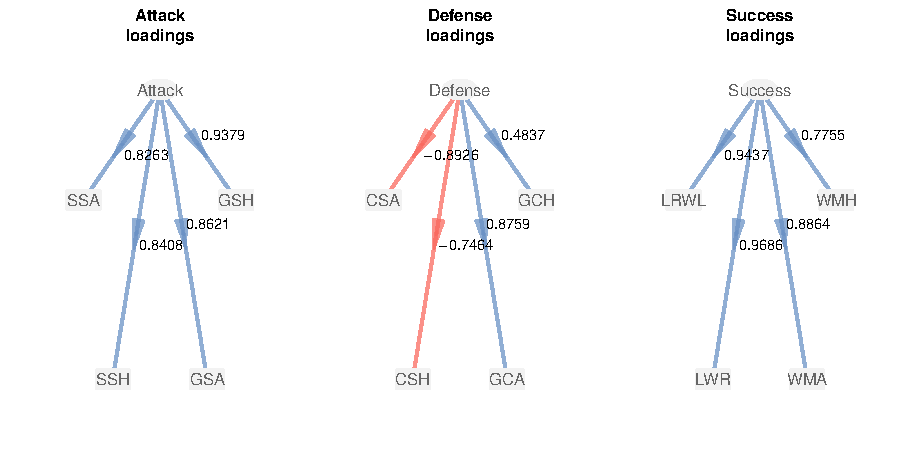
\includegraphics[width=1\linewidth,height=.5\linewidth]{figure/plot_loadings2} 

}



\end{knitrout}

As you can see from the plot, the indicators \texttt{CSA} and \texttt{CSH} have red arrows indicating that they have negative loadings (negative correlations). This can be confirmed if we check the outer model results contained in \code{\$outer\_model}:
\begin{knitrout}
\definecolor{shadecolor}{rgb}{0.969, 0.969, 0.969}\color{fgcolor}\begin{kframe}
\begin{alltt}
\hlcomment{# outer model results}
foot_pls$outer_model
\end{alltt}
\begin{verbatim}
##    name   block  weight loading communality redundancy
## 1   GSH  Attack  0.3366  0.9379      0.8797     0.0000
## 2   GSA  Attack  0.2819  0.8621      0.7432     0.0000
## 3   SSH  Attack  0.2892  0.8408      0.7070     0.0000
## 4   SSA  Attack  0.2396  0.8263      0.6828     0.0000
## 5   GCH Defense -0.1087  0.4837      0.2339     0.0000
## 6   GCA Defense -0.3915  0.8759      0.7672     0.0000
## 7   CSH Defense  0.3274 -0.7464      0.5571     0.0000
## 8   CSA Defense  0.4035 -0.8926      0.7968     0.0000
## 9   WMH Success  0.2309  0.7755      0.6014     0.5145
## 10  WMA Success  0.3030  0.8864      0.7856     0.6722
## 11  LWR Success  0.2821  0.9686      0.9382     0.8027
## 12 LRWL Success  0.2958  0.9437      0.8906     0.7620
\end{verbatim}
\end{kframe}
\end{knitrout}


To get those results associated to the block \code{Defense}, simply use the \code{subset()} function indicating the selection of \code{block == "Defense"}
\begin{knitrout}
\definecolor{shadecolor}{rgb}{0.969, 0.969, 0.969}\color{fgcolor}\begin{kframe}
\begin{alltt}
\hlcomment{# Defense outer model results}
\hlfunctioncall{subset}(foot_pls$outer_model, block == \hlstring{"Defense"})
\end{alltt}
\begin{verbatim}
##   name   block  weight loading communality redundancy
## 5  GCH Defense -0.1087  0.4837      0.2339          0
## 6  GCA Defense -0.3915  0.8759      0.7672          0
## 7  CSH Defense  0.3274 -0.7464      0.5571          0
## 8  CSA Defense  0.4035 -0.8926      0.7968          0
\end{verbatim}
\end{kframe}
\end{knitrout}

Note that we have a weird phenomenon with the signs of the outer weights and the signs of the loadings. You can visualize the weights by using \code{plot()} and specifying the argument \code{what = "weights"} like this:
\begin{knitrout}
\definecolor{shadecolor}{rgb}{0.969, 0.969, 0.969}\color{fgcolor}\begin{kframe}
\begin{alltt}
\hlcomment{# plotting weights}
\hlfunctioncall{plot}(foot_pls, what = \hlstring{"weights"})
\end{alltt}
\end{kframe}

{\centering 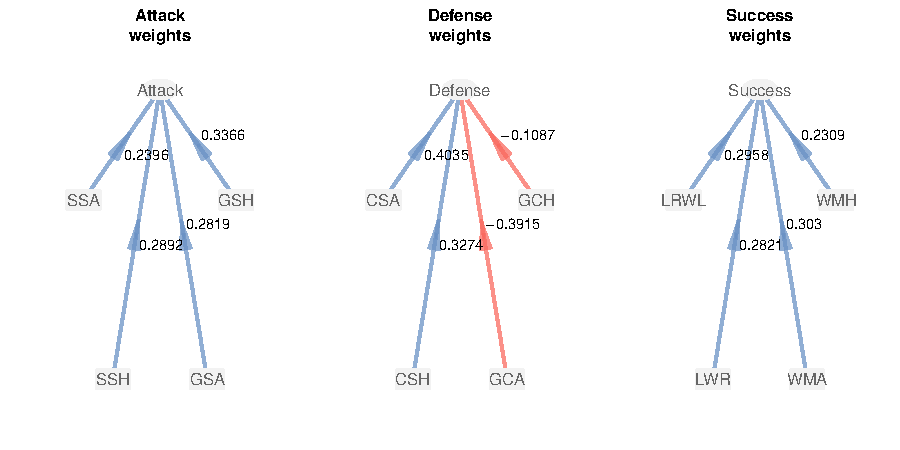
\includegraphics[width=1\linewidth,height=.5\linewidth]{figure/plot_weights} 

}



\end{knitrout}

We have mixed signs: half of the \code{Defense} indicators are positive weights while the other half have negative weights. This is the cause that the Cronbach's alpha and the Dillon-Goldstein's rho are inadequate. Remember that Cronbach's alpha require all indicators in reflective block to be positively correlated. Moreover, this is also the cause that the path coefficient between \code{Defense} and \code{Success} is negative. This is contradictory because it would mean that the more \textit{Quality Defense}, the less \textit{Success}. In fact, this ``anomaly'' of inverted and mixed signs of indicators is not that uncommon. 

Even though \code{GCH} and \code{GCA} have to do with Defense, they are measuring ``lack'' of Defense. If a team has high values of \code{GCH} and \code{GCA}, it means that they conceded a lot of goals, hence having a poor defense quality. Briefly, \code{GCH} and \code{GCA} are pointing in the opposite direction.  We need to do something to try to fix this problem. The solution is to change the sign of \code{GCH} and \code{GCA} so that instead of conceded goals they reflect ``avoided goals''. 


\subsubsection*{Changing \code{Defense} indicators}
One way to have modified the variables \code{GCH} and \code{GCA} with negative signs is by adding two more variables (columns) to the data frame \code{spainfoot}. This can be done like this: 
\begin{knitrout}
\definecolor{shadecolor}{rgb}{0.969, 0.969, 0.969}\color{fgcolor}\begin{kframe}
\begin{alltt}
\hlcomment{# add two more columns NGCH and NGCA}
spainfoot$NGCH = -1 * spainfoot$GCH
spainfoot$NGCA = -1 * spainfoot$GCA
\end{alltt}
\end{kframe}
\end{knitrout}

We are adding a new column \code{NGCH} to \code{spainfoot} calculated as a negative \code{GCH}. This represents \textit{Negative Conceded Goals at Home}. Likewise, we are adding another new column \code{NGCA} (\textit{Negative Goals Conceded Away}) calculated as a negative \code{GCA}. I know that \textit{negative goals conceded at home} and \textit{negative goals conceded away} are not avoided goals, but the idea is to have indicators that are positively related to the \code{Defense} construct. Use either the function \code{names()} or the function \code{colnames()} to check the names of the variables in the data:
\begin{knitrout}
\definecolor{shadecolor}{rgb}{0.969, 0.969, 0.969}\color{fgcolor}\begin{kframe}
\begin{alltt}
\hlcomment{# check column names}
\hlfunctioncall{names}(spainfoot)
\end{alltt}
\begin{verbatim}
##  [1] "GSH"  "GSA"  "SSH"  "SSA"  "GCH"  "GCA"  "CSH"  "CSA"  "WMH" 
## [10] "WMA"  "LWR"  "LRWL" "YC"   "RC"   "NGCH" "NGCA"
\end{verbatim}
\end{kframe}
\end{knitrout}



With the updated data, we have to re-run the \fplspm{} function and we also have to modify the list of blocks with the new indicators \code{NGCH} and \code{NGCA}. You can define the list of \code{blocks} either with numeric vectors or with string vectors. Here's how to define the list of \code{blocks} under both options:
\begin{knitrout}
\definecolor{shadecolor}{rgb}{0.969, 0.969, 0.969}\color{fgcolor}\begin{kframe}
\begin{alltt}
\hlcomment{# new list of blocks (with column positions of variables)}
new_blocks_pos = \hlfunctioncall{list}(1:4, \hlfunctioncall{c}(15,16,7,8), 9:12)

\hlcomment{# new list of blocks (with names of variables)}
new_blocks_str = \hlfunctioncall{list}(
  \hlfunctioncall{c}(\hlstring{"GSH"}, \hlstring{"GSA"}, \hlstring{"SSH"}, \hlstring{"SSA"}), 
  \hlfunctioncall{c}(\hlstring{"NGCH"}, \hlstring{"NGCA"}, \hlstring{"CSH"}, \hlstring{"CSA"}), 
  \hlfunctioncall{c}(\hlstring{"WMH"}, \hlstring{"WMA"}, \hlstring{"LWR"}, \hlstring{"LRWL"}))
\end{alltt}
\end{kframe}
\end{knitrout}


Let's apply \fplspm{} using the list of blocks with the names of the indicators \code{new\_blocks\_str}, and plot the obtained loadings:
\begin{knitrout}
\definecolor{shadecolor}{rgb}{0.969, 0.969, 0.969}\color{fgcolor}\begin{kframe}
\begin{alltt}
\hlcomment{# re-apply plspm}
foot_pls = \hlfunctioncall{plspm}(spainfoot, foot_path, new_blocks_str, modes = foot_modes)

\hlcomment{# plot loadings}
\hlfunctioncall{plot}(foot_pls, \hlstring{"loadings"})
\end{alltt}
\end{kframe}\begin{figure}[h]


{\centering 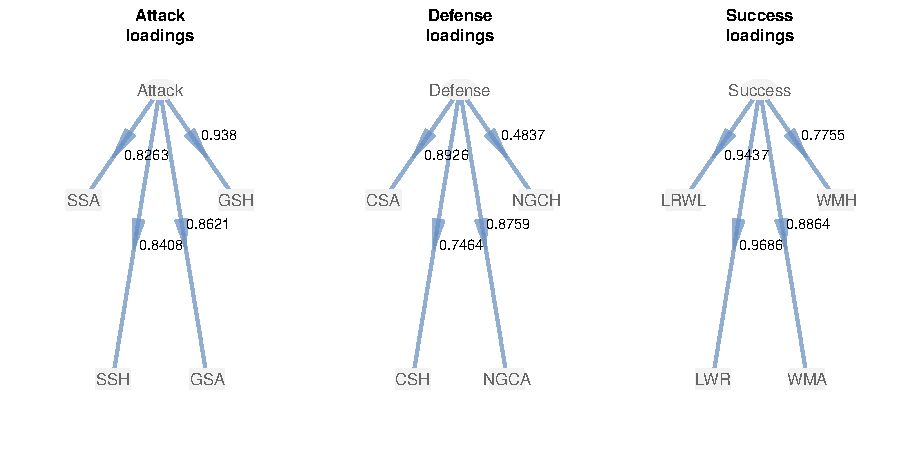
\includegraphics[width=1\linewidth,height=.5\linewidth]{figure/rerun_plspm} 

}

\caption[Changed Loadings]{Changed Loadings\label{fig:rerun_plspm}}
\end{figure}


\end{knitrout}


Now we are talking! As you can tell, all the indicators in \code{Defense} have blue arrows. If we check again the unidimensionality we should see better results:
\begin{knitrout}
\definecolor{shadecolor}{rgb}{0.969, 0.969, 0.969}\color{fgcolor}\begin{kframe}
\begin{alltt}
\hlcomment{# unidimensionality}
foot_pls$unidim
\end{alltt}
\begin{verbatim}
##         Mode MVs C.alpha DG.rho eig.1st eig.2nd
## Attack     A   4  0.8906 0.9246   3.017  0.7923
## Defense    A   4  0.7718 0.8549   2.393  1.1753
## Success    A   4  0.9165 0.9423   3.217  0.5370
\end{verbatim}
\end{kframe}
\end{knitrout}



\subsection{Loadings and Communalities}
The next thing to examine are the loadings and the communalities that are contained in \texttt{\$outer\_model}. The loadings are correlations between a latent variable and its indicators. In turn, communalities are squared correlations.
\begin{knitrout}
\definecolor{shadecolor}{rgb}{0.969, 0.969, 0.969}\color{fgcolor}\begin{kframe}
\begin{alltt}
\hlcomment{# loadings and communalities}
foot_pls$outer_model
\end{alltt}
\begin{verbatim}
##    name   block weight loading communality redundancy
## 1   GSH  Attack 0.3366  0.9380      0.8798     0.0000
## 2   GSA  Attack 0.2819  0.8621      0.7432     0.0000
## 3   SSH  Attack 0.2893  0.8408      0.7070     0.0000
## 4   SSA  Attack 0.2396  0.8263      0.6828     0.0000
## 5  NGCH Defense 0.1088  0.4837      0.2339     0.0000
## 6  NGCA Defense 0.3914  0.8759      0.7672     0.0000
## 7   CSH Defense 0.3274  0.7464      0.5571     0.0000
## 8   CSA Defense 0.4035  0.8926      0.7967     0.0000
## 9   WMH Success 0.2309  0.7755      0.6014     0.5145
## 10  WMA Success 0.3030  0.8864      0.7856     0.6722
## 11  LWR Success 0.2821  0.9686      0.9382     0.8027
## 12 LRWL Success 0.2958  0.9437      0.8906     0.7620
\end{verbatim}
\end{kframe}
\end{knitrout}


In versions of \plspm{} later than 0.4, what we get in \code{foot\_pls\$outer\_model} is a data frame. This allows us to have the output ready for the package \code{ggplot2} and take advatange of its wide range of graphics posibilities. The data frame \code{foot\_pls\$outer\_model} constains five columns. The first column corresponds to the \code{block} which is codified as a \code{factor} (i.e. categorical variable). The second column contains the outer weights. The third column are the loadings (correlations). Loadings greater than 0.7 are acceptable. To see why they are acceptable we use the communalities in the fourth column. Communalities are just squared loadings. They represent the amount of variablity explained by a latent variable. A loading grater than 0.7 means that more than $0.7^2 \approx 50\%$ of the variablity in an indicator is captured by its latent construct. The fifth column are the redundancies; we'll talk about them later in this chapter.

\subsubsection*{Communality}
Communality is calculated with the purpose to check that indicators in a block are well explained by its latent variable. Communalities are simply squared loadings and they measure the part of the variance between a latent variable and its indicator that is common to both. To see why, we need to assume that each indicator represents an error measurement of its construct. The relation:
$$ mv_{jk} = loading_{jk}LV_{j} + error_{jk}$$
implies that the latent variable $LV_j$ explains its indicator $mv_{jk}$, so we have to evaluate how well the indicators are explained by its latent variable. To do this, we examine the loadings which indicate the amount of variance shared between the construct and its indicators. The communality for the $jk$-th manifest variable of the $j$-th block is calculated as:
$$ Com(LV_j, mv_{jk}) = cor^2(LV_j, mv_{jk}) = loading_{jk}^2 $$
Looking at the previous formula, communality measures how much of a given manifest variable's variance is reproducible from the latent variable. In other words, the part of variance between a construct and its indicators that is common to both. One expects to have more shared variance between an LV and its mv than error variance, that is:
$$ loading^2_{jk} > var(error_{jk}) $$
Indicators with low communality are those for which the model is ``not working'' and the researcher may use this information to drop such variables from the analysis.

For instance, let's check what's going on with the \code{Defense} block. The manifest variable \code{GCH} has a loading of 0.4837 which is less than the recommended 0.7. In turn, its communality is small with a value of 0.2339. We should seriously consider whether it makes sense to keep this variable in our model. Although this indicator has some contribution to the \textit{Quality of Defense}, it doesn't seem to be very happy in the \code{Defense} block. If we don't want to have an uncomfortable indicator, the best option is to remove it from the model. For convenience and illustration purposes I'm going to keep \code{GCH} in our exmple, but if you find yourself in the middle of a similar issue, you should talk to the experts and discuss whether to keep or remove unhappy reflective indicators that don't reflect enough.


\subsection{Cross-loadings}
Besides checking the loadings of the indicators with their own latent variables, we must also check the so-called \textit{cross-loadings}. That is, the loadings of an indicator with the rest of latent variables. The reason for doing so is that we need to be sure that we don't have traitor indicators. The data frame of cross-loadings are in \code{\$crossloadings}: 
\begin{knitrout}
\definecolor{shadecolor}{rgb}{0.969, 0.969, 0.969}\color{fgcolor}\begin{kframe}
\begin{alltt}
\hlcomment{# cross-loadings}
foot_pls$crossloadings
\end{alltt}
\begin{verbatim}
##    name   block Attack Defense Success
## 1   GSH  Attack 0.9380  0.5159  0.8977
## 2   GSA  Attack 0.8621  0.3391  0.7519
## 3   SSH  Attack 0.8408  0.4139  0.7714
## 4   SSA  Attack 0.8263  0.3361  0.6390
## 5  NGCH Defense 0.1305  0.4837  0.1598
## 6  NGCA Defense 0.4622  0.8759  0.5751
## 7   CSH Defense 0.3188  0.7464  0.4810
## 8   CSA Defense 0.4215  0.8926  0.5928
## 9   WMH Success 0.7086  0.4226  0.7755
## 10  WMA Success 0.7731  0.7115  0.8864
## 11  LWR Success 0.8444  0.5380  0.9686
## 12 LRWL Success 0.8601  0.5892  0.9437
\end{verbatim}
\end{kframe}
\end{knitrout}


We need to look at the list of results as if it were a super matrix. The way to read the cross-loadings is by looking at this super matrix block by block paying attention to the sections in the diagonal. These sections are the loadings of each block with its construct. A given loading in one of these sections must be greater than any other loading in its row. For example, let's consider the first section that corresponds to the first column in the \code{Attack} block. \code{GSH} has a loading value of 0.9380. This value must be greater than any other value in that first row. The cross-loadings of \code{GSH} with \code{Defense} is 0.5159; the cross-loading of \code{GSH} with \code{Success} is 0.8977. Clearly, 0.9380 is greater than 0.5159 and 0.8977.

An alternative way to examine the table of cross-loadings is by visualizing them with some bar-charts like those shown in the figure below:
\begin{knitrout}
\definecolor{shadecolor}{rgb}{0.969, 0.969, 0.969}\color{fgcolor}

{\centering 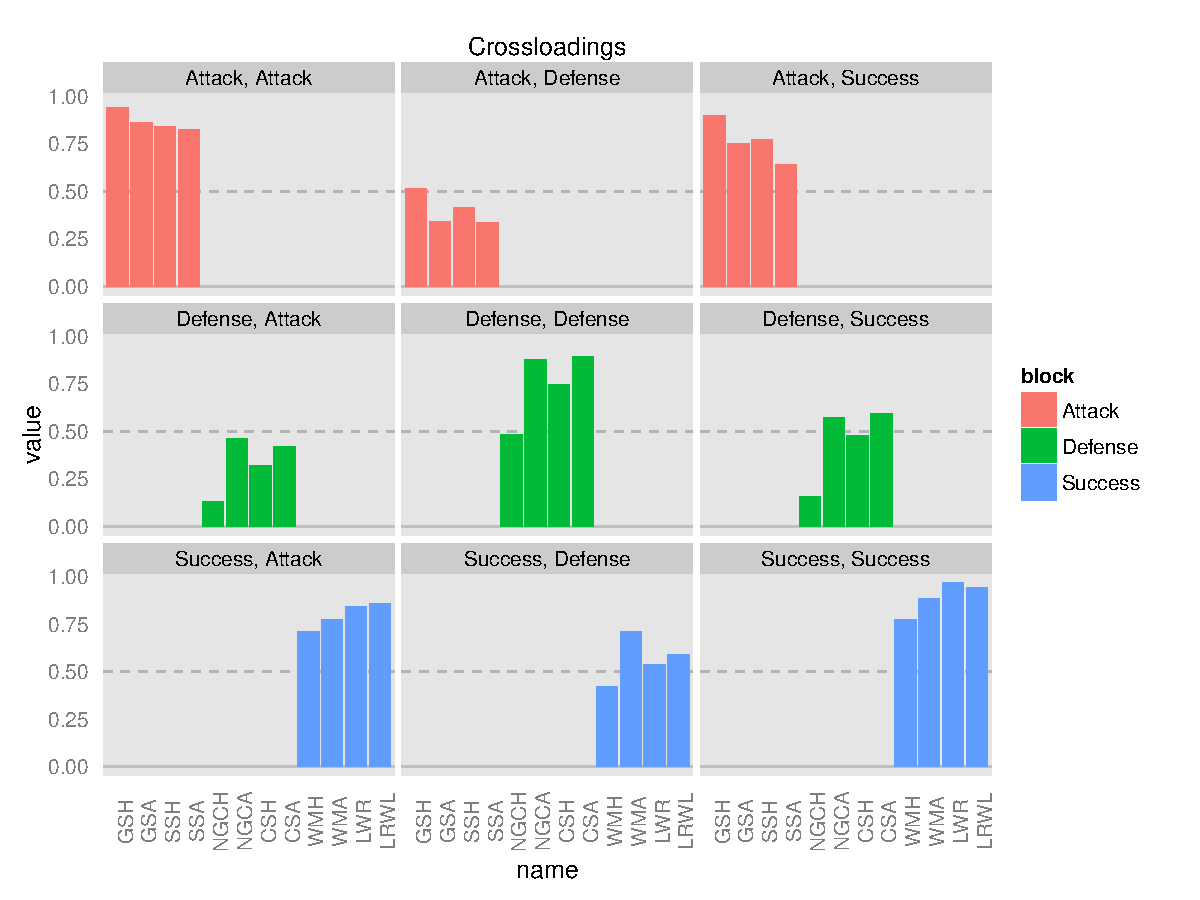
\includegraphics[width=1\linewidth,height=.75\linewidth]{figure/foot_pls_xloads_ggplot} 

}



\end{knitrout}


To get the previous bar-charts we need to use the packages \code{ggplot2} and \code{reshape} (by Hadley Wickham). Once you have installed both packages, the first step is to reformat the data frame of crossloadings. This operation involves using the \code{melt()} function: 
\begin{knitrout}
\definecolor{shadecolor}{rgb}{0.969, 0.969, 0.969}\color{fgcolor}\begin{kframe}
\begin{alltt}
\hlcomment{# load ggplot2 and reshape}
\hlfunctioncall{library}(ggplot2)
\hlfunctioncall{library}(reshape)

\hlcomment{# reshape crossloadings data.frame for ggplot}
xloads = \hlfunctioncall{melt}(foot_pls$crossloadings, id.vars = \hlfunctioncall{c}(\hlstring{"name"}, \hlstring{"block"}),
              variable_name = \hlstring{"LV"})
\end{alltt}
\end{kframe}
\end{knitrout}

The reshaped (i.e. melted) data \code{xloads} is just another \code{data.frame} with the same information as \code{foot\_pls\$crossloadings}. The only difference is in the arrangement of the values so they can meet the required shape for \code{ggplot()}.

After reshaping the data, we can use \code{ggplot()} to produce the bar-charts. To do this, we tell \code{ggplot()} to add bars with \code{geom\_bar()}. Note the use of the parameters \code{stat = 'identity'} and \code{position = 'dodge'}. We also add some horizontal lines as visual references with \code{geom\_hline()}. Then we indicate that we want a panel display with \code{facet\_wrap()} by crossing the loadings of \code{block} with the rest of latent variables (\code{LV}). Finally, we use \code{theme()} to a have a better positioning of the x-axis labels, the size of the title, as well as hiding the grid lines:
\begin{knitrout}
\definecolor{shadecolor}{rgb}{0.969, 0.969, 0.969}\color{fgcolor}\begin{kframe}
\begin{alltt}
\hlcomment{# bar-charts of crossloadings by block}
\hlfunctioncall{ggplot}(data = xloads,
       \hlfunctioncall{aes}(x = name, y = value, fill = block)) +
\hlcomment{  # add horizontal reference lines}
  \hlfunctioncall{geom_hline}(yintercept = 0, color = \hlstring{"gray75"}) + 
  \hlfunctioncall{geom_hline}(yintercept = 0.5, color = \hlstring{"gray70"}, linetype = 2) +
\hlcomment{  # indicate the use of car-charts}
  \hlfunctioncall{geom_bar}(stat = \hlstring{'identity'}, position = \hlstring{'dodge'}) +
\hlcomment{  # panel display (i.e. faceting)}
  \hlfunctioncall{facet_wrap}(block ~ LV) +
\hlcomment{  # tweaking some grahical elements}
  \hlfunctioncall{theme}(axis.text.x = \hlfunctioncall{element_text}(angle = 90),
        line = \hlfunctioncall{element_blank}(),
        plot.title = \hlfunctioncall{element_text}(size = 12)) +
\hlcomment{  # add title}
  \hlfunctioncall{ggtitle}(\hlstring{"Crossloadings"})
\end{alltt}
\end{kframe}
\end{knitrout}


\vspace{3mm}
Keep in mind that cross-loadings allow us to we evaluate the extent to which a given construct differentiates from the others. The whole idea is to verify that the shared variance between a construct and its indicators is larger than the shared variance with other constructs. In other words, no indicator should load higher on another construct than it does on the construct it intends to measure. Otherwise, it is a traitor indicator. If an indicator loads higher with other constructs than the one it is intended to measure, we might consider its appropriateness because it is not clear which construct or constructs it is actually reflecting.



\section{Measurement Model Assessment: \\ Formative Indicators}
Unlike reflective indicators, formative indicators are considered as causing (i.e. forming) a latent variable. The truth is that mathematically, all blocks of indicators could always be taken in a reflective way. However, there may be theoretical or conceptual reasons to consider a block as formative. Formative indicators do not necessarily measure the same underlying construct. In this case, any change experienced by a construct does not imply a change in all its indicators; that is, formative indicators are not supposed to be correlated. For this reason, formative measures cannot be evaluated in the same way of reflective measures; and all the assessment criteria based on the loadings are discarded in the formative measures.

We compare the outer weights of each indicator in order to determine which indicators contribute most effectively to the construct. Attention must be paid in order to avoid misinterpreting relative small absolute values of weights as poor contributions. If we are considering the elimination of some indicator, this should be done based on multicollinearity: the elimination is recommended if high multicollinearity occurs. This implies a strong consensus among experts (based on theory) about how the latent variable is formed.



\section{Structural Model Assessment}
After assessing the quality of the measurement model, the next stage is to assess the structural part. To inspect the results of each regression in the structural equations we need to display the results contained in \code{\$inner\_model}. These results are displayed in a list in the same way as those provided by the function \code{lm()} (i.e. linear model fitting). Since our example has only one regression, we just have one element (\code{\$Success})
\begin{knitrout}
\definecolor{shadecolor}{rgb}{0.969, 0.969, 0.969}\color{fgcolor}\begin{kframe}
\begin{alltt}
\hlcomment{# inner model}
foot_pls$inner_model
\end{alltt}
\begin{verbatim}
## $Success
##             Estimate Std. Error    t value  Pr(>|t|)
## Intercept -2.356e-16    0.09217 -2.556e-15 1.000e+00
## Attack     7.573e-01    0.10440  7.254e+00 1.349e-06
## Defense    2.836e-01    0.10440  2.717e+00 1.466e-02
\end{verbatim}
\end{kframe}
\end{knitrout}


Besides the results of the regression equations, the quality of the structural model is evaluated by examining three indices or quality
metrics:
\begin{itemize}
 \item the $R^2$ determination coefficients
 \item the redundancy index
 \item the Goodness-of-Fit (GoF)
\end{itemize}


\subsection{Coefficients of determination $R^2$}
The $R^2$ are the coefficients of determination of the endogenous latent variables. To inspect these coefficients you need to print the results in \code{\$inner\_summary}.
\begin{knitrout}
\definecolor{shadecolor}{rgb}{0.969, 0.969, 0.969}\color{fgcolor}\begin{kframe}
\begin{alltt}
\hlcomment{# inner model summary}
foot_pls$inner_summary
\end{alltt}
\begin{verbatim}
##               Type     R2 Block_Communality Mean_Redundancy    AVE
## Attack   Exogenous 0.0000            0.7532          0.0000 0.7532
## Defense  Exogenous 0.0000            0.5887          0.0000 0.5887
## Success Endogenous 0.8556            0.8040          0.6878 0.8040
\end{verbatim}
\begin{alltt}

\hlcomment{# select R2}
foot_pls$inner_summary[, \hlstring{"R2"}, drop = FALSE]
\end{alltt}
\begin{verbatim}
##             R2
## Attack  0.0000
## Defense 0.0000
## Success 0.8556
\end{verbatim}
\end{kframe}
\end{knitrout}

For each regression in the structural model we have an $R^2$ that is interpreted similarly as in any multiple regression analysis. $R^2$ indicates the amount of variance in the endogenous latent variable explained by its independent latent variables.

The inner model seems to be fine, although we must keep in mind that this is a very simple model. We have an $R^2 = 0.85$ which under the PLS-PM standards can be considered as an outstanding $R^2$. In fact, values for the R-squared can be classified in three categories (please don't take them as absolute truth):
\begin{enumerate}
 \item Low: $R < 0.30$ (although some authors consider $R<0.20$)
 \item Moderate: $0.30 < R < 0.60$ (you can also find $0.20 < R < 0.50$)
 \item High: $R > 0.60$ (alternatively there's also $R > 0.50$)
\end{enumerate}


\subsection{Redundancy}
Redundancy measures the percent of the variance of indicators in an endogenous block that is predicted from the independent latent variables associated to the endogenous LV. Another definition of redundancy is the amount of variance in an endogenous construct explained by its independent latent variables. In other words, it reflects the ability of a set of independent latent variables to explain variation in the dependent latent variable. The redundancy index for the $j$-th manifest variable associated to the $k$-th block is:
$$ Rd(LV_k, mv_{jk}) = loading^2_{jk} R^2_k $$

High redundancy means high ability to predict. In particular, the researcher may be interested in how well the independent latent variables predict values of the indicators' endogenous construct. Analogous to the communality index, one can calculate the mean redundancy, that is, the average of the redundancy indices of the endogenous blocks.
\begin{knitrout}
\definecolor{shadecolor}{rgb}{0.969, 0.969, 0.969}\color{fgcolor}\begin{kframe}
\begin{alltt}
\hlcomment{# inner model summary}
foot_pls$inner_summary
\end{alltt}
\begin{verbatim}
##               Type     R2 Block_Communality Mean_Redundancy    AVE
## Attack   Exogenous 0.0000            0.7532          0.0000 0.7532
## Defense  Exogenous 0.0000            0.5887          0.0000 0.5887
## Success Endogenous 0.8556            0.8040          0.6878 0.8040
\end{verbatim}
\end{kframe}
\end{knitrout}


For each latent variable we have some descriptive information: type (exogenous or endogenous), measurement (reflective or formative), and number of indicators. The column \texttt{R-square} is only available for endogenous variables. The averga communality \texttt{Av.Commu} indicates how much of the block variability is reproducible by the latent variable. 

Next to the average communality we have the average redundancy \texttt{Av.Redun} which like the R2 is only available for endogenous constructs. \texttt{Av.Redun} represents the percentage of the variance in the endogenous block that is predicted from the indepedent LVs associated to the endogenous LV. High redundancy means high ability to predict. Let's say that we are interested in checking how well the indepedent LVs predict values of endogenous indicators. In our example the average redundancy for Success represents that Attack and Defense predict 68\% of the variability of Success indicators



\subsection{GoF}
A remarkable aspect is that no single criterion exists within the PLS framework to measure the overall quality of a model, so we cannot perform inferential statistical tests for goodness of fit. As an alternative, non-parametrical tests can be applied for the assessment of the structural model.

The GoF index is a pseudo Goodness of fit measure that accounts for the model quality at both the measurement and the structural models. GoF is calculated as the geometric mean of the average communality and the average R2 value. Since it takes in to account communality, this index is more applicable to reflective indicators than to formative indicators. However, you can also use the GoF index in presence of formative blocks, in which case more importance will be given to the average R2.
\begin{knitrout}
\definecolor{shadecolor}{rgb}{0.969, 0.969, 0.969}\color{fgcolor}\begin{kframe}
\begin{alltt}
\hlcomment{# gof index}
foot_pls$gof
\end{alltt}
\begin{verbatim}
## [1] 0.7823
\end{verbatim}
\end{kframe}
\end{knitrout}


GoF can be used a global criterion that helps us to evaluate the performance of the model in both the inner and the outer models. Basically, GoF assess the overall prediction performance of the model. The main drawback with the GoF index is that there is no threshold that allows us to determine its statistical significance. Unfortunately, there is also no guidance about what number could be considered a good GoF value. You can think of GoF as an index of average prediction for the entire model. Although this is not entirely true, it helps to understand GoF values. From this point of view, a GoF value of 0.78 could be interpreted as if the prediction power of the model is of 78\%. The naive rule of thumb is: the higher, the better. Acceptable ``good'' values within the PLS-PM community are GoF \textgreater 0.7


\section{Validation}
Since PLS-PM does not rest on any distributional assumptions, significance levels for the parameter estimates (based on normal theory) are not suitable. Instead, resampling procedures such as blindfolding, jackknifing, and bootstrapping are used to obtain information about the variability of the parameter estimates. \fplspm{} uses the former approach to provide a means for validating results.

\subsection{Bootstrapping}
Bootstrapping is a non-parametric approach for estimating the precision of the PLS parameter estimates. The bootstrap procedure is the following: $M$ samples are created in order to obtain $M$ estimates for each parameter in the PLS model. Each sample is obtained by sampling with replacement from the original data set, with sample size equal to the number of cases in the original data set. 

We use the argument \code{boot.val} to indicate that we wish to perform bootstrap validation. By default \fplspm{} runs 100 resamples but we can specify a different number with the argument \code{br}. For instance, let's get a validation with \code{br=200} resamples. 
\begin{knitrout}
\definecolor{shadecolor}{rgb}{0.969, 0.969, 0.969}\color{fgcolor}\begin{kframe}
\begin{alltt}
\hlcomment{# running bootstrap validation}
foot_val = \hlfunctioncall{plspm}(spainfoot, foot_path, new_blocks_str, modes = foot_modes, 
                 boot.val = TRUE, br = 200)

\hlcomment{# bootstrap results}
foot_val$boot
\end{alltt}
\begin{verbatim}
## $weights
##      Original Mean.Boot Std.Error perc.025 perc.975
## GSH    0.3366   0.33477   0.04699  0.27743   0.4636
## GSA    0.2819   0.26981   0.04893  0.16291   0.3161
## SSH    0.2893   0.29613   0.05155  0.23436   0.4379
## SSA    0.2396   0.23324   0.06251  0.07973   0.2998
## NGCH   0.1088   0.04359   0.18940 -0.33398   0.3306
## NGCA   0.3914   0.37595   0.07005  0.23944   0.4851
## CSH    0.3274   0.28835   0.08725  0.06395   0.4240
## CSA    0.4035   0.41384   0.08603  0.23406   0.5661
## WMH    0.2309   0.23046   0.03723  0.15574   0.2926
## WMA    0.3030   0.30040   0.03109  0.26624   0.3615
## LWR    0.2821   0.28362   0.01688  0.25679   0.3249
## LRWL   0.2958   0.29658   0.02904  0.26279   0.3685
## 
## $loadings
##      Original Mean.Boot Std.Error perc.025 perc.975
## GSH    0.9380    0.9216   0.18909   0.8753   0.9775
## GSA    0.8621    0.8422   0.11750   0.5384   0.9482
## SSH    0.8408    0.8416   0.19186   0.7329   0.9365
## SSA    0.8263    0.8127   0.12381   0.4423   0.9422
## NGCH   0.4837    0.3528   0.37592  -0.4436   0.8846
## NGCA   0.8759    0.8323   0.28609   0.5804   0.9660
## CSH    0.7464    0.6673   0.21917   0.1029   0.9142
## CSA    0.8926    0.8543   0.29122   0.7178   0.9723
## WMH    0.7755    0.7808   0.10617   0.5336   0.9120
## WMA    0.8864    0.8879   0.05111   0.7712   0.9539
## LWR    0.9686    0.9619   0.03415   0.8663   0.9891
## LRWL   0.9437    0.9414   0.03174   0.8660   0.9776
## 
## $paths
##                    Original Mean.Boot Std.Error perc.025 perc.975
## Attack -> Success    0.7573    0.7383     0.174  0.56209   0.9068
## Defense -> Success   0.2836    0.2833     0.115  0.07557   0.4655
## 
## $rsq
##         Original Mean.Boot Std.Error perc.025 perc.975
## Success   0.8556     0.884   0.06458   0.7495   0.9678
## 
## $total.efs
##                    Original Mean.Boot Std.Error perc.025 perc.975
## Attack -> Defense    0.0000    0.0000     0.000  0.00000   0.0000
## Attack -> Success    0.7573    0.7383     0.174  0.56209   0.9068
## Defense -> Success   0.2836    0.2833     0.115  0.07557   0.4655
\end{verbatim}
\end{kframe}
\end{knitrout}

What we obtain in \code{foot\_val\$boot} is a list with results for:
\begin{itemize}
 \item the outer weights (\code{foot\_val\$boot\$weigts})
 \item the loadings (\code{foot\_val\$boot\$loadings})
 \item the path coefficients (\code{foot\_val\$boot\$paths})
 \item the $R^2$ (\code{foot\_val\$boot\$rsq}) 
 \item the total effects (\code{foot\_val\$boot\$total.efs})
\end{itemize}
Each one of these elements is a \code{matrix} that contains five columns: the original value of the parameters, the bootstrap mean value, the bootstrap standard error, and the lower percentile and upper percentiles of the 95\% bootstrap confidence interval.



\section{Reading List}
\begin{itemize}
 \item \textbf{\textsf{How to Write Up and Report PLS Analyses}} by Wynne Chin (2010). This is the Chapter 28 of the \textit{Handbook of Partial Least Squares}. This chapter describes the general steps to be performed for writing a report on results from a PLS-PM analysis.

 \vspace{2mm}
 \item \textbf{\textsf{Evaluation of Structural Equation Models Using Partial Least Squares (PLS) Approach}} by Oliver Gotz, Kerstin Liehr-Gobbers and Manfred Krafft (2010). This is the Chapter 29 of the \textit{Handbook of Partial Least Squares}. Provides a basic comprehension of the PLS-PM methodology and it discussess guidelines for evaluation of structural models.

 \vspace{2mm}
 \item \textbf{\textsf{The Use of Partial Least Squares Path Modeling in International Marketing}} by Jorg Henseler, Christian Ringle and Rudolf R. Sinkovics (2009). This article in \textit{New Challenges to International Marketing Advances in International Marketing (Vol. 20, 277 - 319)} offers guidance for the use of PLS with an emphasis on reasearch studies on marketing research. Covers the requirements, strengths and weaknesses of PLS-PM.

 \vspace{2mm}
 \item \textbf{\textsf{PLS: A Silver Bullet?}} by George A. Marcoulides and Carol Saunders (2006). This is an Editorial comment in the journal \textit{MIS Quarterly (Vol. 30, No. 2)}. The authors express their concerns about claims made by a number of authors about taking PLS as a magic wand that can be applied indiscriminately to all problems.

 \vspace{2mm}
 \item \textbf{\textsf{A Critical Look at Partial Least Squares Modeling}} by George A. Marcoulides, Wynne W. Chin and Carol Saunders (2009). This is the Foreword in the Special Issue Section of the journal \textit{MIS Quarterly (Vol. 33, No. 1, 171-175)}. The authors express their concerns about claims made by a number of authors about taking PLS as a magic wand that can be applied indiscriminately to all problems.
\end{itemize}
  


% Chapter5

% !Rnw root = ../PLS_Path_Modeling_with_R.Rnw


\chapter{Running a PLS-PM Analysis}
In this chapter we are going to carry out a PLS-PM analysis from beginning to end with \plspm{}. The purpose of this exercise is to reproduce, as much as possible, the main steps that you would have to perform in a real life PLS-PM application. As in any data analysis and modeling project, building models is usually the ultimate goal, yet we spend a lot more time understanding the context of the analysis, manipulating the data into the right shape, before we can begin estimating the models. I remember one of my mentors saying that we spend 90\% of the time cleaning and processing the data (I think he underestimated that proportion). As we will find, we prepare the ingredients for our model, do some preliminary check-ups, calculate the model, inspect some results, detect points than need improvement, take a break and get a coffee, then go back to work on the data doing some transformation, formatting, cleaning, build another model, drink more coffee, then return to processing the data once again, and so on for many iterations. In most cases, each cycle takes us a step closer to achieveing a satisfying solution. 

This chapter presents the opportunity to work on a real case study in which we will go through the iterative process required in almost every PLS-PM application. The application is based on a modified Customer Satisfaction model, which is without a doubt \textit{the} standard bearer of the PLS Path Modeling applications. 




\section{Modeling Customer Satisfaction}
We cannot scape the influence \textit{Customer Satisfaction} modeling has had on PLS-PM. Over the last ten years ($\sim$ 2000-2010) many of the successful applications of PLS Path Modeling have been performed within marketing and management studies related with measuring customer satisfaction. It is impossible to deny that this topic has played a key role on the applicability of PLS-PM. Truth be told, Customer Satisfaction Modeling has become the reference application when presenting the PLS path Modeling approach in academic courses, conferences, seminars and workshops. No wonder why Customer Satisfaction Modeling is considered a landmark for PLS-PM as well as an experimental field, becoming the main developmental arena for PLS proposals and innovations.

\subsection{ECSI Model}
Among the large number of available measures of customer satisfaction, we can find the \textbf{European Customer Satisfaction Index} (ECSI). In the late 1990s, the European Union, inspired by the Swedish and the American Customer Satisfaction Indices, started to develop a comparative system of national satisfaction indices. The result was the establishment of the European Customer Satisfaction Index founded by the European Organization for Quality (EOQ), the European Foundation for Quality Management (EFQM) and the European Academic Network for Customer Oriented Quality Analysis (IFCF), with the support of the European Commission and the collaboration of the CSI university network integrated by 8 European universities. 

The ECSI model, illustrated in the diagram below, is designed to measure the cause-effect relationships from the antecedents of \textit{Customer Satisfaction} to its consequences.



\begin{knitrout}
\definecolor{shadecolor}{rgb}{0.969, 0.969, 0.969}\color{fgcolor}\begin{figure}[h]


{\centering 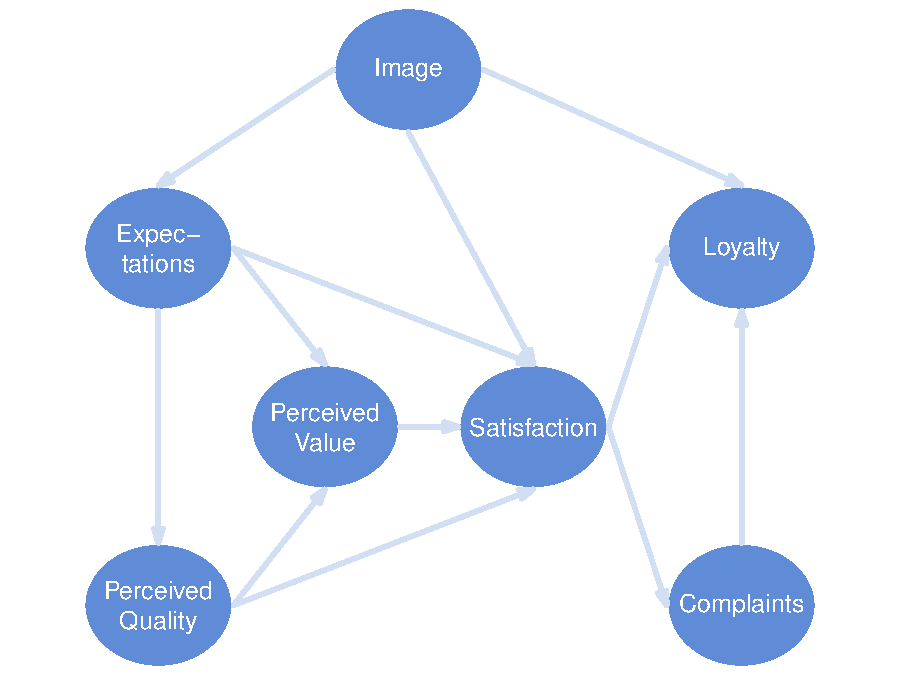
\includegraphics[width=.95\linewidth,height=.5\linewidth]{figure/ECSI_model_diag} 

}

\caption[Diagram of the European Customer Satisfaction Index (ECSI) model]{Diagram of the European Customer Satisfaction Index (ECSI) model\label{fig:ECSI_model_diag}}
\end{figure}


\end{knitrout}


The antecedents of Customer Satisfaction (Image, Expectations, Perceived Quality, and Perceived Value) are the drivers that affect customer satisfaction, while the consequences of customer satisfaction (Loyalty and Complaints) are performance constructs. 

Overview of constructs in the ECSI model:
\begin{itemize}
 \item \textbf{Image} refers to the brand name and the kind of associations customers get from the product/brand/company. It is expected that image will have a positive effect on customer satisfaction and loyalty. In addition, image is also expected to have a direct effect on expectations.
 \item \textbf{Expectations} is the information based on, not actual consumption experienced but, accumulated information about quality from outside sources, such as advertising, word of mouth, and general media.
 \item \textbf{Perceived Quality} comprises product quality (hardware) and service quality (software/humanware). Perceived product quality is the evaluation of recent consumption experience of products. Perceived service quality is the evaluation of recent consumption experience of associated services like customer service, conditions of product display, range of services and products, etc. Perceived quality is expected to affect satisfaction.
 \item \textbf{Perceived Value} is the perceived level of product quality relative to the price paid of the ``value for the money'' aspect of the customer experience.
 \item \textbf{Satisfaction} is defined as an overall evaluation of a firm's post-purchase performance or utilization of a service.
 \item \textbf{Complaints} implies the complaints of customers
 \item \textbf{Loyalty} refers to the intention repurchase and price tolerance of customers. It is the ultimate dependent variable in the model and it is expected that the better image and higher customer satisfaction should increase customer loyalty.
\end{itemize}

\subsection{Case Study: Satisfaction in Education}
The case study for this chapter consists of an application of the ECSI model to Educational Services. The data comes from a survey study made by a student diversity program office in an American university. Typically, this kind of academic programs provide resources to improve the career success of educationally and financially disadvantaged students throughout their college years. In this case study we are going to consider a simplified and modified version of the ECSI model. 

The adapted model aims to measure how satisfied are the members of the program taking into account the quality of the Support provided, the quality of the Advising, and the quality of the Tutoring. It is also supposed that these three quality constructs have an impact on the perceived Value. Besides measuring the satisfaction, the model also pays attention to the Loyalty understood as the commitment and involvement of the students with the program. As we would expect, the more satisfied the members of the program are, the more loyal to the program they will be. The graphical display of the adapted PLS Path Model is shown in the next diagram:
\begin{knitrout}
\definecolor{shadecolor}{rgb}{0.969, 0.969, 0.969}\color{fgcolor}\begin{figure}[h]


{\centering 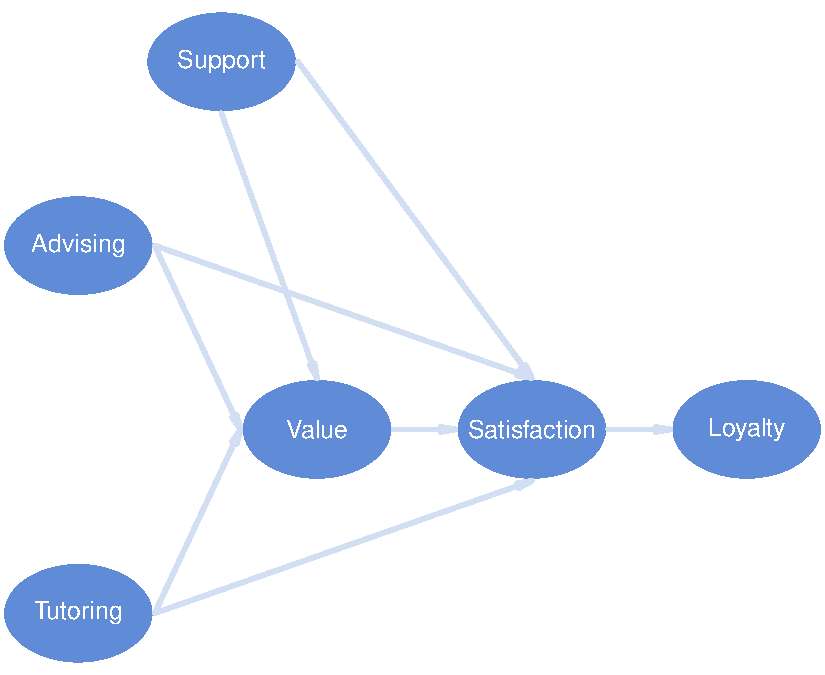
\includegraphics[width=.85\linewidth,height=.5\linewidth]{figure/education_path_diagram} 

}

\caption[Path Diagram of an adapted ECSI model for Educational Services]{Path Diagram of an adapted ECSI model for Educational Services\label{fig:education_path_diagram}}
\end{figure}


\end{knitrout}




\subsubsection*{Data Education}
The dataset for the case study does NOT come with \plspm{}. Since the goal of this chapter is to show you how to use R for running a full PLS Path Modeling analysis, I've decided to go through all the main steps of the analysis process. And that implies that you have to import the dataset in R.

The dataset is available in text format (\code{education.txt}) and in comma separated value format (\code{education.csv}) so you can choose the option that you like the most. Both files can be downloaded from my website:
\begin{itemize}
 \item[] \texttt{\href{http://www.gastonsanchez.com/education.txt}{http://www.gastonsanchez.com/education.txt}}
 \item[] \texttt{\href{http://www.gastonsanchez.com/education.csv}{http://www.gastonsanchez.com/education.csv}}
\end{itemize}
I suggest you to open the downloaded file with your favorite text processor (for the \code{txt} file) or spreadsheet software (for the \code{csv} file) so that you take a quick glance at the data.

\subsubsection*{Importing data in R}
Once you downloaded the file with the \code{education} data, the first step is importing the data in your R session. R comes with various functions to read files. The most common option is to use the function \code{read.table()}, but there are also other sister functions: \code{read.csv()} to read \code{.csv} files, and \code{read.delim()} to read files with other types of delimiters. If you want to know more about importing and exporting data in R, there is a dedicated manual in the CRAN website: \\
\texttt{\href{http://cran.r-project.org/doc/manuals/R-data.html}{http://cran.r-project.org/doc/manuals/R-data.html}} \\
And of course, you can always google for more specific questions.

In my case, I have the data files in my directory \code{"/Users/gaston/PLS"} (the location of the data will be different in your case). Let's see how to read the text file with the function \code{read.table()}:
\begin{knitrout}
\definecolor{shadecolor}{rgb}{0.969, 0.969, 0.969}\color{fgcolor}\begin{kframe}
\begin{alltt}
\hlcomment{# read "education.txt"}
education = \hlfunctioncall{read.table}(\hlstring{"/Users/gaston/PLS/education.txt"}, header = TRUE, 
                       row.names = 1)
\end{alltt}
\end{kframe}
\end{knitrout}

Basically, we are telling \code{read.table()} to read the text file \code{education.txt} located at \code{"/Users/gaston/PLS/education.txt"}. The parameter \code{header=TRUE} indicates that the first row of the data are the column names. In turn, the parameter \code{row.names=1} is used to indicate that the first column contains the names of the rows.

Alternatively, if you prefer to read the \code{.csv} file, you can import the data with the function \code{read.csv()} like this:
\begin{knitrout}
\definecolor{shadecolor}{rgb}{0.969, 0.969, 0.969}\color{fgcolor}\begin{kframe}
\begin{alltt}
\hlcomment{# read "education.csv"}
education = \hlfunctioncall{read.csv}(\hlstring{"/Users/gaston/PLS/education.csv"}, header = TRUE, 
                     row.names = 1)
\end{alltt}
\end{kframe}
\end{knitrout}






If everything went fine, you can use the function \code{dim()} to get the dimensions of the data frame. 
\begin{knitrout}
\definecolor{shadecolor}{rgb}{0.969, 0.969, 0.969}\color{fgcolor}\begin{kframe}
\begin{alltt}
\hlcomment{# how many rows and oclumns?}
\hlfunctioncall{dim}(education)
\end{alltt}
\begin{verbatim}
## [1] 181  26
\end{verbatim}
\end{kframe}
\end{knitrout}


The function \code{summary()} provides basic descriptive statistics of each column:
\begin{knitrout}\small
\definecolor{shadecolor}{rgb}{0.969, 0.969, 0.969}\color{fgcolor}\begin{kframe}
\begin{alltt}
\hlcomment{# summarized statistics of the first 20 columns}
\hlfunctioncall{summary}(education[, 1:20])
\end{alltt}
\begin{verbatim}
##     sup.help      sup.under      sup.safe       sup.conc   
##  Min.   :1.00   Min.   :1.0   Min.   :1.00   Min.   :1.00  
##  1st Qu.:5.00   1st Qu.:1.0   1st Qu.:4.00   1st Qu.:4.00  
##  Median :6.00   Median :2.0   Median :6.00   Median :6.00  
##  Mean   :5.69   Mean   :2.3   Mean   :5.46   Mean   :5.23  
##  3rd Qu.:7.00   3rd Qu.:4.0   3rd Qu.:7.00   3rd Qu.:7.00  
##  Max.   :7.00   Max.   :7.0   Max.   :7.00   Max.   :7.00  
##     adv.comp      adv.acces       adv.comm       adv.qual   
##  Min.   :1.00   Min.   :2.00   Min.   :1.00   Min.   :1.00  
##  1st Qu.:6.00   1st Qu.:6.00   1st Qu.:6.00   1st Qu.:6.00  
##  Median :7.00   Median :7.00   Median :7.00   Median :7.00  
##  Mean   :6.24   Mean   :6.25   Mean   :6.35   Mean   :6.35  
##  3rd Qu.:7.00   3rd Qu.:7.00   3rd Qu.:7.00   3rd Qu.:7.00  
##  Max.   :7.00   Max.   :7.00   Max.   :7.00   Max.   :7.00  
##     tut.prof      tut.sched       tut.stud       tut.qual   
##  Min.   :3.00   Min.   :2.00   Min.   :1.00   Min.   :1.00  
##  1st Qu.:5.00   1st Qu.:5.00   1st Qu.:5.00   1st Qu.:5.00  
##  Median :6.00   Median :6.00   Median :6.00   Median :6.00  
##  Mean   :5.82   Mean   :5.54   Mean   :5.52   Mean   :5.82  
##  3rd Qu.:7.00   3rd Qu.:6.00   3rd Qu.:6.00   3rd Qu.:7.00  
##  Max.   :7.00   Max.   :7.00   Max.   :7.00   Max.   :7.00  
##    val.devel      val.deci       val.meet       val.info   
##  Min.   :1.0   Min.   :1.00   Min.   :1.00   Min.   :2.00  
##  1st Qu.:5.0   1st Qu.:5.00   1st Qu.:5.00   1st Qu.:6.00  
##  Median :6.0   Median :6.00   Median :6.00   Median :6.00  
##  Mean   :5.6   Mean   :5.54   Mean   :5.55   Mean   :6.09  
##  3rd Qu.:7.0   3rd Qu.:7.00   3rd Qu.:7.00   3rd Qu.:7.00  
##  Max.   :7.0   Max.   :7.00   Max.   :7.00   Max.   :7.00  
##     sat.glad       sat.expe       sat.over      loy.proud   
##  Min.   :1.00   Min.   :1.00   Min.   :1.00   Min.   :1.00  
##  1st Qu.:7.00   1st Qu.:6.00   1st Qu.:6.00   1st Qu.:6.00  
##  Median :7.00   Median :7.00   Median :7.00   Median :7.00  
##  Mean   :6.68   Mean   :6.25   Mean   :6.38   Mean   :6.47  
##  3rd Qu.:7.00   3rd Qu.:7.00   3rd Qu.:7.00   3rd Qu.:7.00  
##  Max.   :7.00   Max.   :7.00   Max.   :7.00   Max.   :7.00
\end{verbatim}
\end{kframe}
\end{knitrout}


\subsubsection*{Survey Questionnaire}
Each column in the data is a response of the applied questionnaire to 181 students members of the academic program. There are also three categorical variables (the last three columns): \code{gender}, \code{scholarships}, and \code{job}. They indicate the gender of the respondents, whether they have a scholarship, and whether they have a job. The rest of the questions are measured on a 7-point scale. Depending on the question, the following options were given to the respondents:
\begin{itemize}
 \item[A)] 1 = completely disagree, 4 = neither agree nor disagree, 7 = completely agree
 \item[B)] 1 = not at all, 7 = very much
\end{itemize}

\vspace{2mm}
Below is the list of variables in the data, presented in blocks of indicators with their corresponding question: \\
%\begin{table}[h]
\begin{tabular}{l l}
 \textbf{Support} & \\
 \code{sup.help} & I feel comfortable asking for help from the program's staff \\
 \code{sup.under} & I feel underappreciated in the program \\
 \code{sup.safe} & I can find a place where I feel safe in the program \\
 \code{sup.conc} & I go to the program when I have concerns about school \\
\end{tabular}
%\end{table}

%\begin{table}[h]
\begin{tabular}{l l}
 \textbf{Advising} & \\
 \code{adv.comp} & Competence of advisors \\
 \code{adv.acces} & Access to advisors \\
 \code{adv.comm} & Communication skills of advisors \\
 \code{adv.qual} & Overall quality of advising \\
\end{tabular}
%\end{table}

%\begin{table}[h]
\begin{tabular}{l l}
 \textbf{Tutoring} & \\
 \code{tut.prof} & Proficiency of tutors \\
 \code{tut.sched} & Tutoring schedules \\
 \code{tut.stud} & Variety of study groups \\
 \code{tut.qual} & Overall quality of tutoring \\
\end{tabular}
%\end{table}

%\begin{table}[h]
\begin{tabular}{l l}
 \textbf{Value} & \\
 \code{val.devel} & Helpfulness in my personal development \\
 \code{val.deci} & Helpfulness in personal decision making \\
 \code{val.meet} & Facilitating meeting people and contacts \\
 \code{val.info} & Accessibility to support and information \\
\end{tabular}
%\end{table}

%\begin{table}[h]
\begin{tabular}{l l}
 \textbf{Satisfaction} & \\
 \code{sat.glad} & I'm glad to be a member of the program \\
 \code{sat.expe} & The program meets my expectations \\
 \code{sat.over} & Overall, I'm very satisfied with the program \\
\end{tabular}
%\end{table}

%\begin{table}[h]
\begin{tabular}{l l}
 \textbf{Loyalty} & \\
 \code{loy.proud} & I'm proud to tell others I'm part of the program \\
 \code{loy.recom} & I would recommend the program to my colleagues \\
 \code{loy.asha} & I often feel ashamed of being a member of the program \\
 \code{loy.back} & I'm interested in giving something back to the program \\
\end{tabular}
%\end{table}



\section{Preliminary Exploration}
The dataset is already clean and shaped in the right format, which will save us a lot of time dealing with the boring part of data pre-processing. As you can tell, the variables are already named according the their corresponding blocks. However, we still have to work on a couple of preparatory tasks before playing with the \fplspm{} function. So let us start with some preliminary analysis by exploring the dataset and the blocks of variables.

\subsection{Looking at the data}
First we will perform some visual explorations. We can calculate the distribution values with the function \code{table()} and then apply \code{barplot()} to get a bar chart. This is how we do it with the first variable \code{sup.help}:
\begin{knitrout}
\definecolor{shadecolor}{rgb}{0.969, 0.969, 0.969}\color{fgcolor}\begin{kframe}
\begin{alltt}
\hlcomment{# distribution of first column}
aux_distrib = \hlfunctioncall{table}(education[, 1])/\hlfunctioncall{nrow}(education)

\hlcomment{# barplot of the distribution}
\hlfunctioncall{barplot}(aux_distrib, border = NA, main = \hlfunctioncall{colnames}(education)[1])
\end{alltt}
\end{kframe}\begin{figure}[h]


{\centering 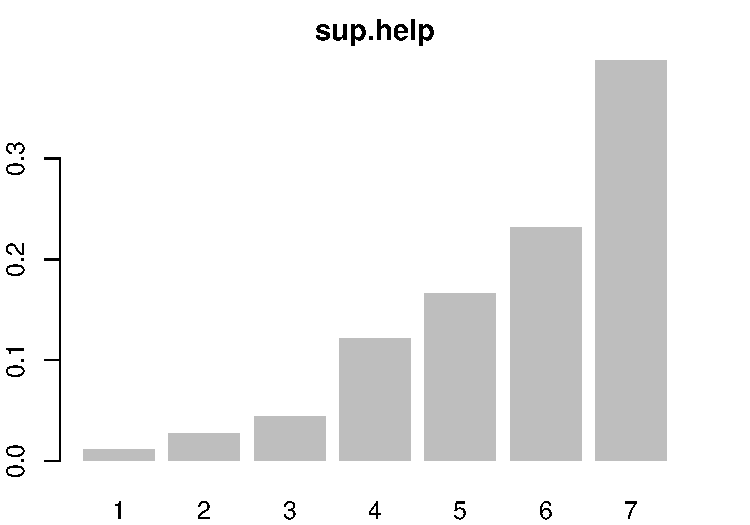
\includegraphics[width=.55\linewidth,height=.4\linewidth]{figure/support_mvs_distrs} 

}

\caption[Visualizing the distribution of the first Support indicator]{Visualizing the distribution of the first Support indicator\label{fig:support_mvs_distrs}}
\end{figure}


\end{knitrout}


Because we have four manifest variables related to \code{Support}, it would be nice to visualize the distributions of all the indicators. Most of the graphics that we do are for purely inspection purposes. But then we need to prepare some plots in a nicer way to be included in a report or a presentation. Say we want to get more beautiful charts than the default options provided by \code{barplot()}. We can use the colors in the package \code{RColorBrewer} (by Erich Neuwirth):
\begin{knitrout}
\definecolor{shadecolor}{rgb}{0.969, 0.969, 0.969}\color{fgcolor}\begin{kframe}
\begin{alltt}
\hlcomment{# package RColorBrewer (for nice colors)}
\hlfunctioncall{library}(RColorBrewer)
\end{alltt}
\end{kframe}
\end{knitrout}


We will also need to have better column labels instead of the column names in the data \code{education}. Let's create a vector with names for the indicators of \code{Support}:
\begin{knitrout}
\definecolor{shadecolor}{rgb}{0.969, 0.969, 0.969}\color{fgcolor}\begin{kframe}
\begin{alltt}
\hlcomment{# questions of Support indicators}
sq1 = \hlstring{"Help when not doing well"}
sq2 = \hlstring{"I feel underappreciated"}
sq3 = \hlstring{"I can find a place where I feel safe"}
sq4 = \hlstring{"Concerns about school"}

\hlcomment{# put questions in one vector}
sup_questions = \hlfunctioncall{c}(sq1, sq2, sq3, sq4)
\end{alltt}
\end{kframe}
\end{knitrout}


Here's the figure with the bar charts of the manifest variables in \code{Support}:
\begin{knitrout}
\definecolor{shadecolor}{rgb}{0.969, 0.969, 0.969}\color{fgcolor}\begin{figure}[h]


{\centering 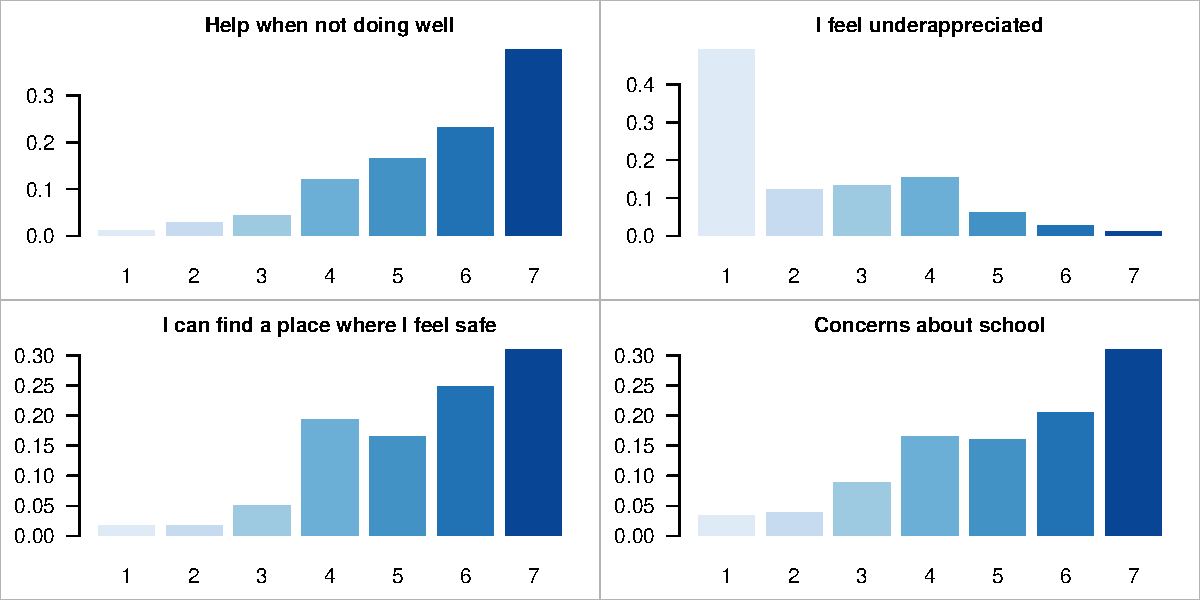
\includegraphics[width=1\linewidth,height=.6\linewidth]{figure/barplots_support_figure} 

}

\caption[Visualizing the distributions of Support indicators]{Visualizing the distributions of Support indicators\label{fig:barplots_support_figure}}
\end{figure}


\end{knitrout}


How do we get such a nice graphic? Here is the code to get pretty barplots of the first block of manifest variables: 
\begin{knitrout}
\definecolor{shadecolor}{rgb}{0.969, 0.969, 0.969}\color{fgcolor}\begin{kframe}
\begin{alltt}
\hlcomment{# setting graphical parameters}
op = \hlfunctioncall{par}(mfrow = \hlfunctioncall{c}(2,2), mar = \hlfunctioncall{c}(2.5, 3.2, 2, 0.8))
\hlcomment{# bar-chart for each indicator of Support}
\hlfunctioncall{for} (j in 1:4) \{
  distribution = \hlfunctioncall{table}(education[,j]) / \hlfunctioncall{nrow}(education)
  \hlfunctioncall{barplot}(distribution, border = NA, col = \hlfunctioncall{brewer.pal}(8, \hlstring{"Blues"})[2:8], 
          axes = FALSE, main = sup_questions[j], cex.main = 1)
\hlcomment{  # add vertical axis, and rectangle around figure}
  \hlfunctioncall{axis}(side = 2, las=2)
  \hlfunctioncall{box}(\hlstring{"figure"}, col=\hlstring{"gray70"})
\}
\hlcomment{# reset default graphical parameters}
\hlfunctioncall{par}(op)
\end{alltt}
\end{kframe}
\end{knitrout}


To plot the distributions in a single graphic window, we use the function \code{par()} to set the graphical parameters \code{mfrow} and \code{mar}. The parameter \code{mfrow} allows to set a layout with a vector specifying the number of rows and columns. The parameter \code{mar} sets the margins of the figures. In order to plot each barchart we apply a \code{for} loop that goes from the first to the fourth column in the dataset. Notice that inside \code{barplot()} we are using \code{brewer.pal()} to specify the color palette \code{"Blues"}. In addition, we are using \code{axis()} to manipulate the vertical axis and show its numbers in a horizontal way (which makes it easier to read the numbers). Finally, \code{box()} is used to plot the gray frame around each single figure. Your turn: try to plot the distributions of all blocks of indicators in \code{education}.

If we pay attention to the barplots associated with \code{Support}, we should be able to see a clear pattern: the distributions are skewed, either to the left or to the right. This is something very common when working with people's perceptions where they tend to agree or disagree in a strong way. The other pattern has to do with the question ``I feel underappreciated in the program''. Notice that its distribution is concentrated in the lower values of the scale, specially on 1. Can you guess why is this happening?



\subsection{Seeing the forest, not just the trees}
The barplots are a good means to have a better idea of what the data look like. But if we want to have a deeper understanding of the data we have to take a next step: \textbf{correlations}. Calculating correlations allows us to get a feeling of the relationships between the variables. Let's examine the correlations of the manifest variables integrating the \code{Support} block:
\begin{knitrout}
\definecolor{shadecolor}{rgb}{0.969, 0.969, 0.969}\color{fgcolor}\begin{kframe}
\begin{alltt}
\hlcomment{# correlations of Support indicators}
\hlfunctioncall{cor}(education[, 1:4])
\end{alltt}
\begin{verbatim}
##           sup.help sup.under sup.safe sup.conc
## sup.help    1.0000   -0.4056   0.5234   0.5383
## sup.under  -0.4056    1.0000  -0.3883  -0.2927
## sup.safe    0.5234   -0.3883   1.0000   0.3710
## sup.conc    0.5383   -0.2927   0.3710   1.0000
\end{verbatim}
\end{kframe}
\end{knitrout}


Is there anything that calls your attention? Notice that \code{sup.under} is negatively correlated with the rest of indicators in the block \code{Support}. Jointly with the correlations, we can also make use of Principal Component Analysis (PCA) in an attempt to appreciate the systematic patterns in the data that are hard to see with the naked eye. We will perform a PCA with the function \code{nipals()} available in the package \code{plsdepot} (rememeber to install it first with \code{install.packages()}):
\begin{knitrout}
\definecolor{shadecolor}{rgb}{0.969, 0.969, 0.969}\color{fgcolor}\begin{kframe}
\begin{alltt}
\hlcomment{# load plsdepot}
\hlfunctioncall{library}(plsdepot)

\hlcomment{# PCA of Support indicators with nipals}
support_pca = \hlfunctioncall{nipals}(education[,1:4])

\hlcomment{# plot}
\hlfunctioncall{plot}(support_pca, main = \hlstring{"Support \hlfunctioncall{indicators} (circle of correlations)"}, 
     cex.main = 1)
\end{alltt}
\end{kframe}\begin{figure}[h]


{\centering 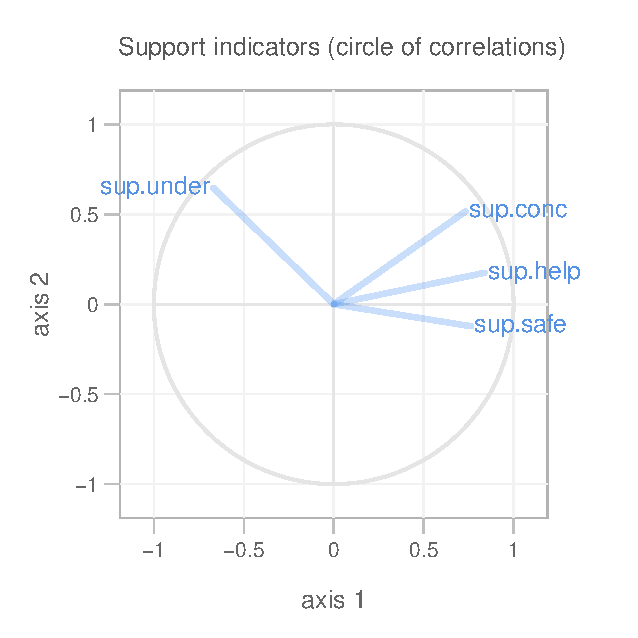
\includegraphics[width=.55\linewidth,height=.55\linewidth]{figure/support_nipals} 

}

\caption[Visualizing the correlations of Support indicators]{Visualizing the correlations of Support indicators\label{fig:support_nipals}}
\end{figure}


\end{knitrout}


This graphic is known as a \textbf{circle of correlations} and is just a representation of the variable correlations on the first two principal axes associated with the first two principal components. You can read this graphic as if it were a radar. While the indicators \code{sup.conc}, \code{sup.help} and \code{sup.safe} are somewhat clustered on the right, the variable \code{sup.under} is in the upper-left corner. The fact that \code{sup.under} is on the left compared to the other indicators, reflects the fact of being negatively correlated with them. Why do we have this ``anomaly''? The answer can be found if we look at the second question associated to \code{Support}: \textit{I feel underappreciated in the program}. Clearly, this question is not measuring Support but rather Lack of Support. Right now we are not going to do anything with this issue, although you should keep it in mind (we'll talk about it in the next section).

For the sake of convenience I'm not going to perform more PCA's on the rest of blocks of manifest variables. However, I encourage you to try to do the same exploratory analysis. This is something that eventually you will have to do in any real life situation, and it will save you further headaches when cooking your PLS path models.



\section{PLS-PM Round 1}
Let us assume that we have completed the exploratory phase of the manifest variables and that everything seems to be reasonably OK. This would mean that we did our homework by cleaning the data, treating missing values, deciding what to do with the outliers, formatting those variables that needed some transformations, and so on. We are now ready for the main show: the PLS Path Model building part. To start our model building process, we need to prepare the main ingredients for \fplspm{}: the \code{path\_matrix}, the list of \code{blocks}, and the vector \code{modes}.




\subsubsection*{Inner model: \code{path\_matrix}}
The path matrix of our model can be defined as:
\begin{knitrout}
\definecolor{shadecolor}{rgb}{0.969, 0.969, 0.969}\color{fgcolor}\begin{kframe}
\begin{alltt}
\hlcomment{# rows of path matrix}
Support = \hlfunctioncall{c}(0, 0, 0, 0, 0, 0)
Advising = \hlfunctioncall{c}(0, 0, 0, 0, 0, 0)
Tutoring = \hlfunctioncall{c}(0, 0, 0, 0, 0, 0)
Value = \hlfunctioncall{c}(1, 1, 1, 0, 0, 0)
Satisfaction = \hlfunctioncall{c}(1, 1, 1, 1, 0, 0)
Loyalty = \hlfunctioncall{c}(0, 0, 0, 0, 1, 0)

\hlcomment{# matrix (by row binding)}
edu_path = \hlfunctioncall{rbind}(Support, Advising, Tutoring, Value, Satisfaction, Loyalty)

\hlcomment{# add column names (optional)}
\hlfunctioncall{colnames}(edu_path) = \hlfunctioncall{rownames}(edu_path)
\end{alltt}
\end{kframe}
\end{knitrout}


We can check the \code{path\_matrix} in path diagram version with \code{innerplot()}. This will help you to inspect the model and see if it is well defined:
\begin{knitrout}
\definecolor{shadecolor}{rgb}{0.969, 0.969, 0.969}\color{fgcolor}\begin{kframe}
\begin{alltt}
\hlcomment{# plot the inner matrix}
\hlfunctioncall{innerplot}(edu_path, box.size = 0.1)
\end{alltt}
\end{kframe}\begin{figure}[h]


{\centering 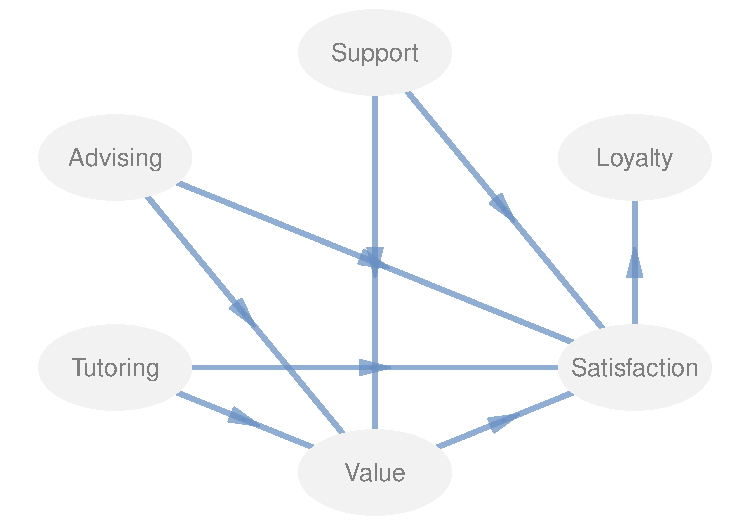
\includegraphics[width=.8\linewidth,height=.5\linewidth]{figure/edu_innerplot} 

}

\caption[Visualizing the path diagram of the inner model with innerplot]{Visualizing the path diagram of the inner model with innerplot\label{fig:edu_innerplot}}
\end{figure}


\end{knitrout}


\subsubsection*{Outer model: \code{blocks} and \code{modes}}
The second ingredient for \fplspm{} is the list defining the blocks of the measurement (outer) model and the measurement type to be used (reflective indicators in this case):
\begin{knitrout}
\definecolor{shadecolor}{rgb}{0.969, 0.969, 0.969}\color{fgcolor}\begin{kframe}
\begin{alltt}
\hlcomment{# outer model}
edu_blocks = \hlfunctioncall{list}(1:4, 5:8, 9:12, 13:16, 17:19, 20:23)

\hlcomment{# modes (reflective blocks)}
edu_modes = \hlfunctioncall{rep}(\hlstring{"A"}, 6)
\end{alltt}
\end{kframe}
\end{knitrout}


\subsubsection*{Applying \fplspm{}}
Once we have the required ingredients, we can apply \fplspm{}. Since this is our first attempt, we will use \fplspm{} with its default arguments. We will later ask for bootstrap validation.
\begin{knitrout}
\definecolor{shadecolor}{rgb}{0.969, 0.969, 0.969}\color{fgcolor}\begin{kframe}
\begin{alltt}
\hlcomment{# apply plspm}
edu_pls1 = \hlfunctioncall{plspm}(education, edu_path, edu_blocks, modes = edu_modes)

\hlcomment{# print edu_pls1}
edu_pls1
\end{alltt}
\begin{verbatim}
## Partial Least Squares Path Modeling (PLS-PM) 
## ---------------------------------------------
##    NAME             DESCRIPTION
## 1  $outer_model     outer model
## 2  $inner_model     inner model
## 3  $path_coefs      path coefficients matrix
## 4  $scores          latent variable scores
## 5  $crossloadings   cross-loadings
## 6  $inner_summary   summary inner model
## 7  $effects         total effects
## 8  $unidim          unidimensionality
## 9  $gof             goodness-of-fit
## 10 $boot            bootstrap results
## 11 $data            data matrix
## ---------------------------------------------
## You can also use the function 'summary'
\end{verbatim}
\end{kframe}
\end{knitrout}

As you know, you can use the function \code{summary()} to display all the results of the model in the screen of your R session. For illustration purposes I won't use \code{summary()} but instead will go step by step with the results contained in \code{edu\_pls1}:


\subsubsection*{Unidimensionality of Reflective Blocks}
The diagnosis of a PLS path model begins with assessing the quality of the measurement model. Since we have reflective indicators, we must chek the unidimensionality of the blocks. Unidimensionality implies that the reflective indicators must be in a geometrical space of one dimension. Remember that manifest variables in a reflective block are considered as being caused by their latent variable (i.e. reflective manifest variables are indicating the same latent variable). In PLS-PM we have three main indices to check unidimensionality: 1) the Cronbach's alpha, 2) the Dillon-Goldstein's rho, and 3) the first eigenvalue of the MVs correlation matrix:
\begin{knitrout}
\definecolor{shadecolor}{rgb}{0.969, 0.969, 0.969}\color{fgcolor}\begin{kframe}
\begin{alltt}
\hlcomment{# check unidimensionality}
edu_pls1$unidim
\end{alltt}
\begin{verbatim}
##              Mode MVs C.alpha DG.rho eig.1st eig.2nd
## Support         A   4  0.1967 0.6158   2.271  0.7292
## Advising        A   4  0.9283 0.9492   3.296  0.3430
## Tutoring        A   4  0.8545 0.9021   2.791  0.5377
## Value           A   4  0.9103 0.9371   3.154  0.5090
## Satisfaction    A   3  0.9025 0.9390   2.511  0.2700
## Loyalty         A   4  0.3383 0.7223   2.623  0.6791
\end{verbatim}
\end{kframe}
\end{knitrout}


Looking at the table in \code{edu\_pls1\$unidim}, most of the blocks seem to have acceptable values (greater than 0.7) for the Cronbach's alpha and Dillon-Goldstein's rho. However, \code{Support} and \code{Loyalty} present low alphas of 0.1967 and 0.3383, respectively. To have a better idea of what's going on with the indicators in the ``problematic'' blocks, let's plot the loadings
\begin{knitrout}
\definecolor{shadecolor}{rgb}{0.969, 0.969, 0.969}\color{fgcolor}\begin{kframe}
\begin{alltt}
\hlcomment{# plotting the loadings}
\hlfunctioncall{plot}(edu_pls1, what = \hlstring{"loadings"})
\end{alltt}
\end{kframe}\begin{figure}[h]


{\centering 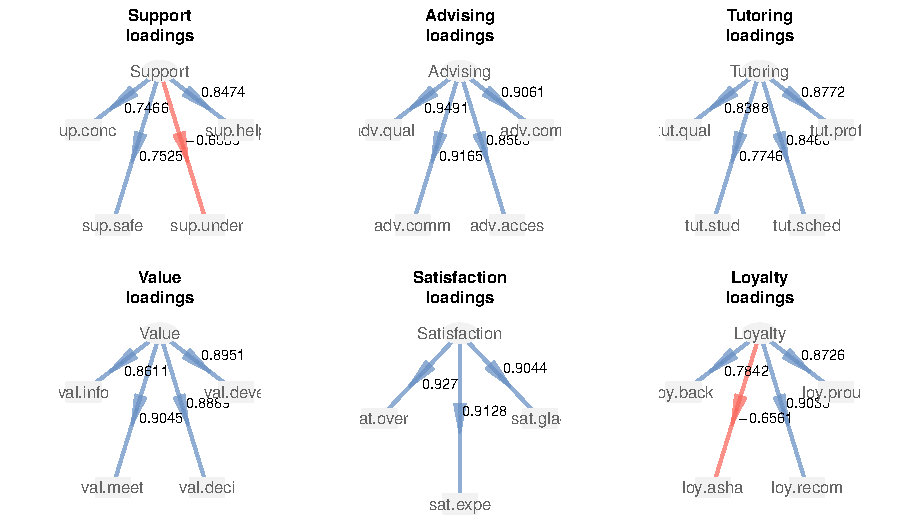
\includegraphics[width=1\linewidth,height=.6\linewidth]{figure/edu_pls1_loadings_plot} 

}

\caption[Visualizing the loadings (correlations)]{Visualizing the loadings (correlations)\label{fig:edu_pls1_loadings_plot}}
\end{figure}


\end{knitrout}


It turns out that the variable \code{sup.under} has a negative loading with \code{Support}. This corresponds to what we saw earlier in section 2 of this chapter. In addition, the variable \code{loy.asha} presents the same issue in the block of \code{Loyalty}. Although these two blocks can be considered as unidimensional, they both have an indicator that is not pointing in the same direction as the other indicators in each block. What would you do to fix this problem?




\section{PLS-PM Round 2}
We need to change the indicators \code{sup.under} and \code{loy.asha}. The question behind \code{sup.under} is: ``I feel underappreciated in the program''. The question behind \code{loy.asha} is: ``I often feel ashamed of the program''. Thus, instead of ``I feel underappreciated'' we would like to have ``I feel appreciated''. In the same way, instead of ``I often feel ashamed of being a member of the program'', we would like to have ``I feel pleased of being a member of the program''. 

This issue is more common than you think. You would be surprised by how many times I've seen this ``anomaly'' when analyzing others researchers' data. This is obviously not a problem of PLS or any other structural equation modeling approach. This is an issue that has to do with survey desings, more specifically with the designing of the questions. That's why is so crucial to get familiar with your data and do the exploratory analysis so you don't get caught unguarded with this type of phenomenon. I know that we already had detected the problem with \code{sup.under}, but I wanted to get to this point so you could see one of the many fault-prone components that you will encounter when applying PLS-PM.

The proposed solution is to invert the scale of the ill-fated manifest variables. Actually, the proposal consists of creating new indicators that we may call \code{sup.appre} (I feel \textit{appreciated} in the program) and \code{loy.pleas} (I feel \textit{pleased} of being a member of the program). Here is how you can create the new indicators and add them to \code{education}:
\begin{knitrout}
\definecolor{shadecolor}{rgb}{0.969, 0.969, 0.969}\color{fgcolor}\begin{kframe}
\begin{alltt}
\hlcomment{# adding Support 'appreciated'}
education$sup.appre = 8 - education$sup.under

\hlcomment{# adding 'Loyalty' pleased}
education$loy.pleas = 8 - education$loy.asha
\end{alltt}
\end{kframe}
\end{knitrout}

We take the number 8 and we subtract the original values. In this way, when we had a value of 1 we now have a value of 7. Conversely, when we had a 7 we now have a 1.

Let's apply \fplspm{} again. Of all the ingredients, we need to re-specify the outer list because of the two new indicators that we just aggregated to the data frame:
\begin{knitrout}
\definecolor{shadecolor}{rgb}{0.969, 0.969, 0.969}\color{fgcolor}\begin{kframe}
\begin{alltt}
\hlcomment{# outer model 2}
edu_blocks2 = \hlfunctioncall{list}(\hlfunctioncall{c}(1, 27, 3, 4), 5:8, 9:12, 13:16, 17:19, \hlfunctioncall{c}(20, 21, 28, 
    23))

\hlcomment{# apply plspm}
edu_pls2 = \hlfunctioncall{plspm}(education, edu_path, edu_blocks2, modes = edu_modes)
\end{alltt}
\end{kframe}
\end{knitrout}


As we did in the last section, we can visualize the loadings in each block and make sure that this time all the arrows are colored in blue, meaning positive correlations (i.e. loadings):
\begin{knitrout}
\definecolor{shadecolor}{rgb}{0.969, 0.969, 0.969}\color{fgcolor}\begin{kframe}
\begin{alltt}
\hlcomment{# plotting the loadings}
\hlfunctioncall{plot}(edu_pls2, what = \hlstring{"loadings"})
\end{alltt}
\end{kframe}\begin{figure}[h]


{\centering 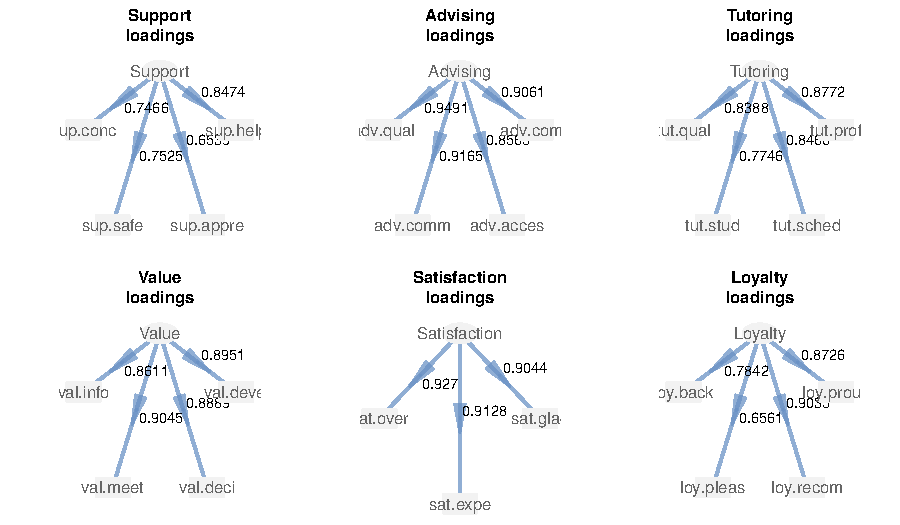
\includegraphics[width=1\linewidth,height=.6\linewidth]{figure/edu_pls2_loadings_plot} 

}

\caption[Visualizing loadings - round 2]{Visualizing loadings - round 2\label{fig:edu_pls2_loadings_plot}}
\end{figure}


\end{knitrout}


And we check the blocks' unidimensionality:
\begin{knitrout}
\definecolor{shadecolor}{rgb}{0.969, 0.969, 0.969}\color{fgcolor}\begin{kframe}
\begin{alltt}
\hlcomment{# check unidimensionality}
edu_pls2$unidim
\end{alltt}
\begin{verbatim}
##              Mode MVs C.alpha DG.rho eig.1st eig.2nd
## Support         A   4  0.7433 0.8392   2.271  0.7292
## Advising        A   4  0.9283 0.9492   3.296  0.3430
## Tutoring        A   4  0.8545 0.9021   2.791  0.5377
## Value           A   4  0.9103 0.9371   3.154  0.5090
## Satisfaction    A   3  0.9025 0.9390   2.511  0.2700
## Loyalty         A   4  0.8200 0.8827   2.623  0.6791
\end{verbatim}
\end{kframe}
\end{knitrout}

By using the modified indicators with inverted scales, we have managed to solve the issue with the unidimensionality of the blocks. Now \code{Support} has a Cronbach's alpha of 0.7433 and \code{Loyalty} has a corresponding alpha of 0.82. 


\subsubsection*{Loadings and Communalities}
Besides plotting the loadings, we need to do a more careful inspection by checking the results contained in \code{\$outer\_model}:
\begin{knitrout}
\definecolor{shadecolor}{rgb}{0.969, 0.969, 0.969}\color{fgcolor}\begin{kframe}
\begin{alltt}
\hlcomment{# check outer model}
edu_pls2$outer_model
\end{alltt}
\begin{verbatim}
##         name        block weight loading communality redundancy
## 1   sup.help      Support 0.3870  0.8474      0.7181     0.0000
## 2  sup.appre      Support 0.2741  0.6539      0.4275     0.0000
## 3   sup.safe      Support 0.3173  0.7525      0.5663     0.0000
## 4   sup.conc      Support 0.3404  0.7466      0.5574     0.0000
## 5   adv.comp     Advising 0.2652  0.9061      0.8210     0.0000
## 6  adv.acces     Advising 0.2572  0.8565      0.7336     0.0000
## 7   adv.comm     Advising 0.2879  0.9165      0.8400     0.0000
## 8   adv.qual     Advising 0.2903  0.9491      0.9008     0.0000
## 9   tut.prof     Tutoring 0.3023  0.8772      0.7695     0.0000
## 10 tut.sched     Tutoring 0.3154  0.8466      0.7168     0.0000
## 11  tut.stud     Tutoring 0.2975  0.7746      0.6000     0.0000
## 12  tut.qual     Tutoring 0.2830  0.8388      0.7035     0.0000
## 13 val.devel        Value 0.2628  0.8951      0.8012     0.5195
## 14  val.deci        Value 0.2759  0.8889      0.7902     0.5124
## 15  val.meet        Value 0.2739  0.9045      0.8181     0.5304
## 16  val.info        Value 0.3156  0.8611      0.7415     0.4808
## 17  sat.glad Satisfaction 0.3543  0.9044      0.8179     0.5144
## 18  sat.expe Satisfaction 0.3550  0.9128      0.8331     0.5240
## 19  sat.over Satisfaction 0.3835  0.9270      0.8594     0.5406
## 20 loy.proud      Loyalty 0.3334  0.8726      0.7614     0.4591
## 21 loy.recom      Loyalty 0.3513  0.9035      0.8163     0.4922
## 22 loy.pleas      Loyalty 0.2423  0.6561      0.4305     0.2596
## 23  loy.back      Loyalty 0.2968  0.7842      0.6150     0.3708
\end{verbatim}
\end{kframe}
\end{knitrout}

What we get is a data frame with the outer weights, the loadings (correlations), the communalities and the redundancies. Acceptable values for the loadings are values greater than 0.7. Equivalently, communalities values greater than $0.7^2 = 0.49$ are considered as acceptable. Because communalities represent the amount of variablity explained by a latent variable, a communality greater than 0.5 means that more than 50\% of the variablity in an indicator is captured by its latent construct. 

Since the output of the outer model is a data frame, we can take advantage of the package \code{ggplot2} to produce a bar chart of loadings (or communalitites). Here's an option to visualize the loadings (remember to install \code{ggplot2} if you haven't done it):
\begin{knitrout}
\definecolor{shadecolor}{rgb}{0.969, 0.969, 0.969}\color{fgcolor}\begin{kframe}
\begin{alltt}
\hlcomment{# load ggplot2}
\hlfunctioncall{library}(ggplot2)

\hlcomment{# barchart of loadings}
\hlfunctioncall{ggplot}(data = edu_pls2$outer_model, 
       \hlfunctioncall{aes}(x = name, y = loading, fill = block)) +
  \hlfunctioncall{geom_bar}(stat = \hlstring{'identity'}, position = \hlstring{'dodge'}) +
\hlcomment{  # threshold line (to peek acceptable loadings above 0.7)}
  \hlfunctioncall{geom_hline}(yintercept = 0.7, color = \hlstring{'gray50'}) +
\hlcomment{  # add title}
  \hlfunctioncall{ggtitle}(\hlstring{"Barchart of Loadings"}) +
\hlcomment{  # rotate x-axis names}
  \hlfunctioncall{theme}(axis.text.x = \hlfunctioncall{element_text}(angle = 90))
\end{alltt}
\end{kframe}

{\centering 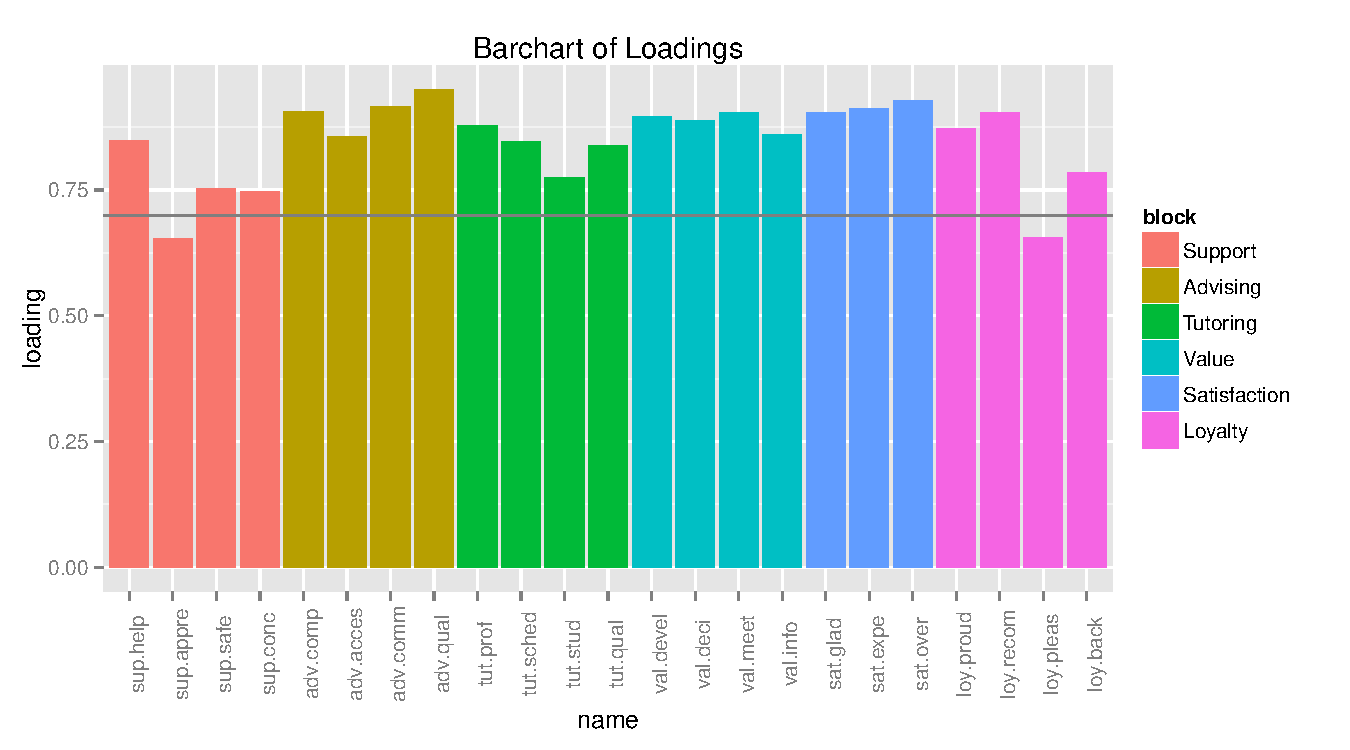
\includegraphics[width=1\linewidth,height=.6\linewidth]{figure/edu_pls2_barplot_loadings} 

}



\end{knitrout}


Notice that the \code{Support} indicator \code{sup.appre} has a loading of 0.6539 (below the gray horizontal line). Likewise, the \code{Loyalty} indicator \code{loy.pleas} has a loading of 0.6561. These loadings are below the recommended threshold of 0.7. Actually, these are the modified indicators that we included in the data and it seems that they are not happy indicators. Whether you decide to keep them or remove them is up to many things. Are they really important for the model? Are they really relevant in the theory used to propose the model? What do the experts that you are working with have to say? Could you replace them with other indicators? These are some of the question that you have to face in cases like this one. Being this a tutorial example, I propose to ban the unhappy indicators and re-run again our PLS path model without \code{sup.appre} and \code{loy.pleas}.




\section{PLS-PM Round 3}
We said in this chapter's introduction that data analysis and model building is an iterative process. The myth of applying any method in a straightforward way is just that: a myth. We have tried to estimate two PLS models without much ``success''. But you should know that this is totally fine, after all we are just getting a little bit closer to our goal. This is a trial and error process that may require transforming and merging data, redefine the model, remove some observations, and sometimes even get more data with better quality. In real life I would recommend you to stop for a while, take a break, go for a walk. After that, we can go back to work and redefine the list of \code{blocks} and re-apply \fplspm{} one more time:
\begin{knitrout}
\definecolor{shadecolor}{rgb}{0.969, 0.969, 0.969}\color{fgcolor}\begin{kframe}
\begin{alltt}
\hlcomment{# outer model 3}
edu_blocks3 = \hlfunctioncall{list}(\hlfunctioncall{c}(1, 3, 4), 5:8, 9:12, 13:16, 17:19, \hlfunctioncall{c}(20, 21, 23))

\hlcomment{# re-apply plspm}
edu_pls3 = \hlfunctioncall{plspm}(education, edu_path, edu_blocks3, modes = edu_modes)
\end{alltt}
\end{kframe}
\end{knitrout}


\subsection{Checking unidimensionality}
As it is customary, we begin by checking the blocks' unidimensionality:
\begin{knitrout}
\definecolor{shadecolor}{rgb}{0.969, 0.969, 0.969}\color{fgcolor}\begin{kframe}
\begin{alltt}
\hlcomment{# check unidimensionality}
edu_pls3$unidim
\end{alltt}
\begin{verbatim}
##              Mode MVs C.alpha DG.rho eig.1st eig.2nd
## Support         A   3  0.7328 0.8492   1.959  0.6293
## Advising        A   4  0.9283 0.9492   3.296  0.3430
## Tutoring        A   4  0.8545 0.9021   2.791  0.5377
## Value           A   4  0.9103 0.9371   3.154  0.5090
## Satisfaction    A   3  0.9025 0.9390   2.511  0.2700
## Loyalty         A   3  0.8454 0.9071   2.297  0.4889
\end{verbatim}
\end{kframe}
\end{knitrout}

Everything looks fine: both the Croncbach's alphas and the Dillon-Goldstein's rhos are greater than 0.7. Regarding the eigen-analysis, the first eigenvalues are much more larger than 1, while the second eigenvalues are smaller than 1, which is taken as evidence that the variables in each block live in a more-or-less unidimensional space.


\subsection{Loadings and Communalities}
We then proceed with evaluating the loadings and communalities. This time all the indicators in each block should be happy indicators: loadings greater than 0.7 and communalities greater than 0.49:
\begin{knitrout}
\definecolor{shadecolor}{rgb}{0.969, 0.969, 0.969}\color{fgcolor}\begin{kframe}
\begin{alltt}
\hlcomment{# check outer model}
edu_pls3$outer_model
\end{alltt}
\begin{verbatim}
##         name        block weight loading communality redundancy
## 1   sup.help      Support 0.4571  0.8697      0.7563     0.0000
## 2   sup.safe      Support 0.3747  0.7631      0.5823     0.0000
## 3   sup.conc      Support 0.4021  0.7872      0.6197     0.0000
## 4   adv.comp     Advising 0.2652  0.9061      0.8210     0.0000
## 5  adv.acces     Advising 0.2572  0.8565      0.7336     0.0000
## 6   adv.comm     Advising 0.2879  0.9165      0.8400     0.0000
## 7   adv.qual     Advising 0.2903  0.9491      0.9008     0.0000
## 8   tut.prof     Tutoring 0.3024  0.8772      0.7695     0.0000
## 9  tut.sched     Tutoring 0.3154  0.8466      0.7168     0.0000
## 10  tut.stud     Tutoring 0.2974  0.7746      0.6000     0.0000
## 11  tut.qual     Tutoring 0.2830  0.8388      0.7035     0.0000
## 12 val.devel        Value 0.2637  0.8956      0.8021     0.5304
## 13  val.deci        Value 0.2764  0.8893      0.7908     0.5229
## 14  val.meet        Value 0.2743  0.9044      0.8180     0.5408
## 15  val.info        Value 0.3137  0.8604      0.7403     0.4895
## 16  sat.glad Satisfaction 0.3579  0.9053      0.8196     0.5120
## 17  sat.expe Satisfaction 0.3543  0.9125      0.8326     0.5201
## 18  sat.over Satisfaction 0.3807  0.9264      0.8582     0.5361
## 19 loy.proud      Loyalty 0.3874  0.8873      0.7872     0.4595
## 20 loy.recom      Loyalty 0.4082  0.9246      0.8549     0.4990
## 21  loy.back      Loyalty 0.3447  0.8089      0.6544     0.3819
\end{verbatim}
\end{kframe}
\end{knitrout}



\subsubsection*{Cross-lodadings}
After checking the loadings of the indicators with their own latent variables, we continue with inspecting the so-called \textbf{cross-loadings}. That is, the loadings of an indicator with the rest of latent variables. The reason why we check this is because we don't want traitor indicators:
\begin{knitrout}\small
\definecolor{shadecolor}{rgb}{0.969, 0.969, 0.969}\color{fgcolor}\begin{kframe}
\begin{alltt}
\hlcomment{# check cross loadings}
edu_pls3$crossloadings
\end{alltt}
\begin{verbatim}
##         name        block Support Advising Tutoring  Value Satisfaction Loyalty
## 1   sup.help      Support  0.8697   0.4719   0.4003 0.7006       0.5593  0.4888
## 2   sup.safe      Support  0.7631   0.2819   0.3365 0.5568       0.4762  0.3452
## 3   sup.conc      Support  0.7872   0.3762   0.4243 0.6523       0.4563  0.4168
## 4   adv.comp     Advising  0.3927   0.9061   0.4028 0.4546       0.5919  0.4154
## 5  adv.acces     Advising  0.3898   0.8565   0.3848 0.4493       0.5654  0.3813
## 6   adv.comm     Advising  0.4830   0.9165   0.4450 0.5122       0.6240  0.4660
## 7   adv.qual     Advising  0.4447   0.9491   0.4730 0.4976       0.6479  0.4824
## 8   tut.prof     Tutoring  0.3955   0.4793   0.8772 0.4105       0.4399  0.4423
## 9  tut.sched     Tutoring  0.4329   0.3453   0.8466 0.4375       0.4496  0.4373
## 10  tut.stud     Tutoring  0.3964   0.3487   0.7746 0.4010       0.4356  0.3631
## 11  tut.qual     Tutoring  0.3734   0.4018   0.8388 0.3657       0.4302  0.3740
## 12 val.devel        Value  0.6939   0.4424   0.3642 0.8956       0.5583  0.5087
## 13  val.deci        Value  0.7173   0.4649   0.4303 0.8893       0.5454  0.4743
## 14  val.meet        Value  0.6956   0.4027   0.4085 0.9044       0.6345  0.5034
## 15  val.info        Value  0.6983   0.5497   0.5031 0.8604       0.6983  0.5808
## 16  sat.glad Satisfaction  0.5328   0.5493   0.4573 0.5760       0.9053  0.8199
## 17  sat.expe Satisfaction  0.5839   0.5808   0.4751 0.6425       0.9125  0.6236
## 18  sat.over Satisfaction  0.5779   0.7033   0.5099 0.6759       0.9264  0.6556
## 19 loy.proud      Loyalty  0.4172   0.3690   0.3857 0.4596       0.6796  0.8873
## 20 loy.recom      Loyalty  0.4730   0.4623   0.4463 0.5220       0.7160  0.9246
## 21  loy.back      Loyalty  0.4807   0.4374   0.4466 0.5641       0.6046  0.8089
\end{verbatim}
\end{kframe}
\end{knitrout}

Remember that you need to look at the list of results as if it were a super matrix: read it block by block paying attention to the sections in the diagonal. These sections are the loadings of each block with its construct. A given loading in one of these sections must be greater than any other loading in its row. For example, let's consider the last section that corresponds to \code{Loyalty}. The last column in this section has the loadings of the manifest variables in \code{Loyalty}. Let's focus on the first indicator \code{loy.proud} that has a loading of 0.8873. All of its cross-loadings are smaller than 0.8873, which is good. If you do the same check-up for \code{loy.recom} and \code{loy.back}, you should see that all their cross-loadings are below their respective loadings.

What if an indicator loads higher with other constructs than the one it is intended to measure? Then you must consider whether it is appropriate to include it in the model. A hesitant indicator that is not clear which construct or constructs it is actually reflecting is not well seen. Reflective indicators need to get along with its latent variable; they must show sings of membership and belonging to one and only one latent variable: they need to be loyal to its construct. If one indicator loads higher on another construct, this could be evidence of treason. We don't want traitor indicators, we want loyal indicators.



\subsection{Path Coefficients}
After assessing the quality of the outer model, then we can turn into the inner model to check its quality. We may start evaluating the structural results by taking a peek at the path coefficients using the \code{plot()} function:
\begin{knitrout}
\definecolor{shadecolor}{rgb}{0.969, 0.969, 0.969}\color{fgcolor}\begin{kframe}
\begin{alltt}
\hlcomment{# plotting results (inner model)}
\hlfunctioncall{plot}(edu_pls3)
\end{alltt}
\end{kframe}\begin{figure}[h]


{\centering 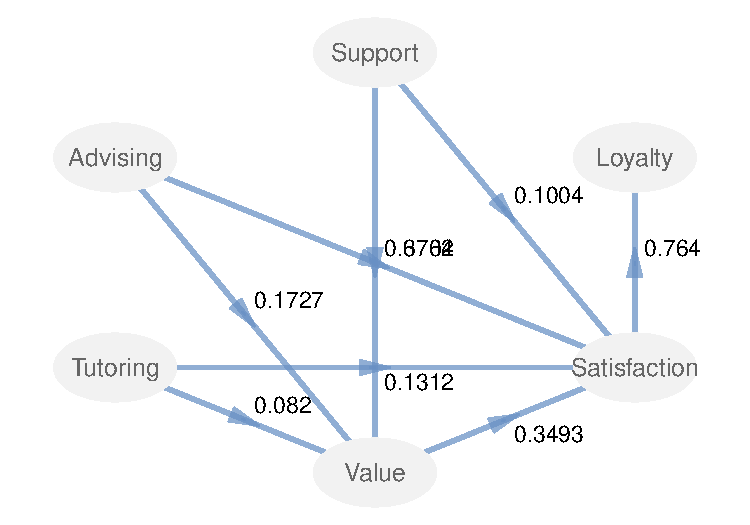
\includegraphics[width=.8\linewidth,height=.5\linewidth]{figure/edu_pls3_plot_inner1} 

}

\caption[Inner model with path coefficients]{Inner model with path coefficients\label{fig:edu_pls3_plot_inner1}}
\end{figure}


\end{knitrout}

As you can see from the previous plot, we have an issue with the arrows from \code{Support} to \code{Value} and from \code{Advising} to \code{Satisfaction}. The problem is that the path coefficients on these arrows are overlapped and it's impossible to distinguish them. We can also inspect the coefficients directly on the matrix of path coefficients:
\begin{knitrout}
\definecolor{shadecolor}{rgb}{0.969, 0.969, 0.969}\color{fgcolor}\begin{kframe}
\begin{alltt}
\hlcomment{# matrix of path coefficients}
edu_pls3$path_coefs
\end{alltt}
\begin{verbatim}
##              Support Advising Tutoring  Value Satisfaction Loyalty
## Support       0.0000   0.0000  0.00000 0.0000        0.000       0
## Advising      0.0000   0.0000  0.00000 0.0000        0.000       0
## Tutoring      0.0000   0.0000  0.00000 0.0000        0.000       0
## Value         0.6702   0.1727  0.08196 0.0000        0.000       0
## Satisfaction  0.1004   0.3764  0.13121 0.3493        0.000       0
## Loyalty       0.0000   0.0000  0.00000 0.0000        0.764       0
\end{verbatim}
\end{kframe}
\end{knitrout}


Even though we have the matrix of path coefficients, it would still be good to visualize the coefficients on the path diagram without the overlapping inconvenient. This can be easily solved using the arrow position argument \code{arr.pos} inside the \code{plot()} function. The default value of this argument is \code{arr.pos = 0.5} indicating that the arrowhead is located at the middle of the arrow. Try a different value to modify the position:
\begin{knitrout}
\definecolor{shadecolor}{rgb}{0.969, 0.969, 0.969}\color{fgcolor}\begin{kframe}
\begin{alltt}
\hlcomment{# plotting results (inner model)}
\hlfunctioncall{plot}(edu_pls3, arr.pos = 0.35)
\end{alltt}
\end{kframe}\begin{figure}[h]


{\centering 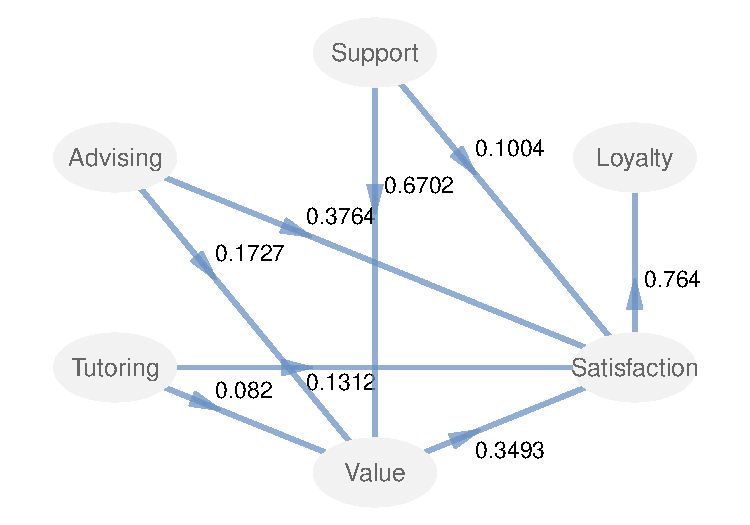
\includegraphics[width=.8\linewidth,height=.5\linewidth]{figure/edu_pls3_plot_inner2} 

}

\caption[Slightly changing the location of the path coefficients]{Slightly changing the location of the path coefficients\label{fig:edu_pls3_plot_inner2}}
\end{figure}


\end{knitrout}


We can obtain another interesting display by using the parameter \code{arr.lwd} inside the \code{plot()} function. This parameter allows us to modify the line width of the arrows between any two latent variables. By default \code{arr.lwd = 3}, but we can specify a matrix like the matrix of path coefficients (\code{\$path\_coefs}) with different values for each arrow. Here is an example of how can we define such a matrix:
\begin{knitrout}
\definecolor{shadecolor}{rgb}{0.969, 0.969, 0.969}\color{fgcolor}\begin{kframe}
\begin{alltt}
\hlcomment{# matrix of path coefficients}
Paths = edu_pls3$path_coefs

\hlcomment{# matrix with values based on path coeffs}
arrow_lwd = 10 * \hlfunctioncall{round}(Paths, 2)

\hlcomment{# how does it look like?}
arrow_lwd
\end{alltt}
\begin{verbatim}
##              Support Advising Tutoring Value Satisfaction Loyalty
## Support          0.0      0.0      0.0   0.0          0.0       0
## Advising         0.0      0.0      0.0   0.0          0.0       0
## Tutoring         0.0      0.0      0.0   0.0          0.0       0
## Value            6.7      1.7      0.8   0.0          0.0       0
## Satisfaction     1.0      3.8      1.3   3.5          0.0       0
## Loyalty          0.0      0.0      0.0   0.0          7.6       0
\end{verbatim}
\end{kframe}
\end{knitrout}


Let us see the effect that \code{arrow\_lwd} has on the size of each arrow:
\begin{knitrout}
\definecolor{shadecolor}{rgb}{0.969, 0.969, 0.969}\color{fgcolor}\begin{kframe}
\begin{alltt}
\hlcomment{# arrows of different sizes reflecting the values of the path coeffs}
\hlfunctioncall{plot}(edu_pls3, arr.pos = 0.35, arr.lwd = arrow_lwd)
\end{alltt}
\end{kframe}\begin{figure}[h]


{\centering 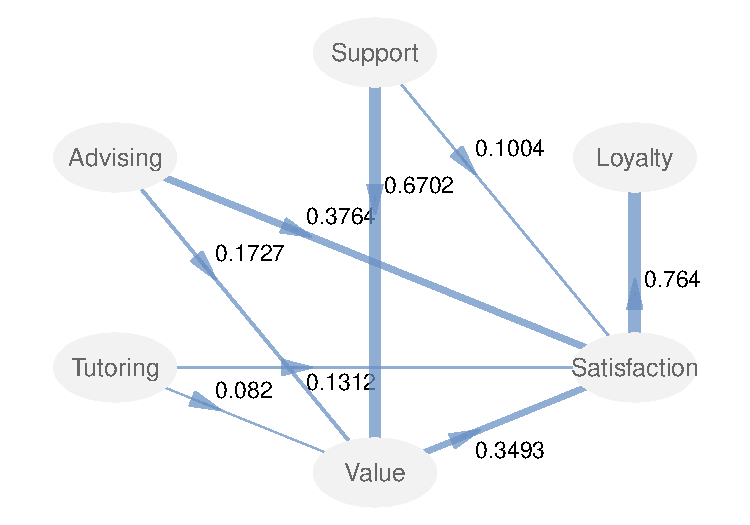
\includegraphics[width=.8\linewidth,height=.5\linewidth]{figure/edu_pls3_plot_inner3} 

}

\caption[Line width of arrows reflecting the magnitude of the path coefficients]{Line width of arrows reflecting the magnitude of the path coefficients\label{fig:edu_pls3_plot_inner3}}
\end{figure}


\end{knitrout}




\subsection{Structural Regressions}
In addition to inspecting the path coefficients, we must also review the regression results of each endogenous construct. This implies examining the regressions for \code{Value}, \code{Satisfaction}, and \code{Loyalty}. To check the inner regressions we print the output of \code{\$inner\_model}:
\begin{knitrout}
\definecolor{shadecolor}{rgb}{0.969, 0.969, 0.969}\color{fgcolor}\begin{kframe}
\begin{alltt}
\hlcomment{# inner model}
edu_pls3$inner_model
\end{alltt}
\begin{verbatim}
## $Value
##             Estimate Std. Error    t value  Pr(>|t|)
## Intercept -7.645e-17    0.04375 -1.747e-15 1.000e+00
## Support    6.702e-01    0.05260  1.274e+01 8.311e-27
## Advising   1.727e-01    0.05233  3.301e+00 1.166e-03
## Tutoring   8.196e-02    0.05256  1.559e+00 1.207e-01
## 
## $Satisfaction
##            Estimate Std. Error   t value  Pr(>|t|)
## Intercept 1.804e-16    0.04618 3.906e-15 1.000e+00
## Support   1.004e-01    0.07688 1.306e+00 1.931e-01
## Advising  3.764e-01    0.05691 6.614e+00 4.324e-10
## Tutoring  1.312e-01    0.05586 2.349e+00 1.993e-02
## Value     3.493e-01    0.07934 4.402e+00 1.853e-05
## 
## $Loyalty
##              Estimate Std. Error   t value  Pr(>|t|)
## Intercept    2.54e-16    0.04823 5.266e-15 1.000e+00
## Satisfaction 7.64e-01    0.04823 1.584e+01 6.765e-36
\end{verbatim}
\end{kframe}
\end{knitrout}

The \code{R2} values are the coefficients of determination of the endogenous latent variables. For each regression in the structural model we have an $R^2$ that is interpreted similarly as in any multiple regression analysis. $R^2$ indicates the amount of variance in the endogenous latent variable explained by its independent latent variables.


\subsection{Effects}
Another interesting result to pay attention to is the table of \code{\$effects}. This table contains the effects that each construct has on the rest of constructs by taking into consideration the total number of connections in the inner model. The direct effects are given by the path coefficients. But there are also the indirect effects and the total effects. An indirect effect is the influence of one construct on another construct by taking an indirect path. The total effects are the sum of both the direct and indirect effects: 
\begin{knitrout}
\definecolor{shadecolor}{rgb}{0.969, 0.969, 0.969}\color{fgcolor}\begin{kframe}
\begin{alltt}
\hlcomment{# effects}
edu_pls3$effects
\end{alltt}
\begin{verbatim}
##               relationships  direct indirect   total
## 1       Support -> Advising 0.00000  0.00000 0.00000
## 2       Support -> Tutoring 0.00000  0.00000 0.00000
## 3          Support -> Value 0.67021  0.00000 0.67021
## 4   Support -> Satisfaction 0.10043  0.23408 0.33452
## 5        Support -> Loyalty 0.00000  0.25557 0.25557
## 6      Advising -> Tutoring 0.00000  0.00000 0.00000
## 7         Advising -> Value 0.17273  0.00000 0.17273
## 8  Advising -> Satisfaction 0.37640  0.06033 0.43673
## 9       Advising -> Loyalty 0.00000  0.33365 0.33365
## 10        Tutoring -> Value 0.08196  0.00000 0.08196
## 11 Tutoring -> Satisfaction 0.13121  0.02863 0.15983
## 12      Tutoring -> Loyalty 0.00000  0.12211 0.12211
## 13    Value -> Satisfaction 0.34927  0.00000 0.34927
## 14         Value -> Loyalty 0.00000  0.26683 0.26683
## 15  Satisfaction -> Loyalty 0.76398  0.00000 0.76398
\end{verbatim}
\end{kframe}
\end{knitrout}

The indirect effects are obtained as the product of the path coefficients by taking an indirect path. For instance, consider the impact of \code{Value} on \code{Loyalty}. Even though these two constructs are not directly connected, there is an indirect path from \code{Value} to \code{Loyalty} that goes through \code{Satisfaction}. If you multiply the path coefficient of \code{Value} on \code{Satisfaction} (0.3493) with the path coefficient of \code{Satisfaction} on \code{Loyalty} (0.764), you get the indirect effect of \code{Value} on \code{Loyalty}: 0.2668 = 0.3493 x 0.764.

\subsubsection{Visualizing the Effects}
A useful and nicer way to inspect the combined effects is by using the graphic capabilities of R to produce a bar chart with the function \code{barplot()}. To create the barplot of effects we first select the ``active'' rows from \code{edu\_pls3\$effects}. We can do this by creating a vector with those rows from the data frame of effects that contain direct and indirect effects (we don't want the uninteresting rows full with zeros).
\begin{knitrout}
\definecolor{shadecolor}{rgb}{0.969, 0.969, 0.969}\color{fgcolor}\begin{kframe}
\begin{alltt}
\hlcomment{# selecting effects ('active' rows)}
good_rows = \hlfunctioncall{c}(3:5, 7:15)

\hlcomment{# 'active' effects in matrix format}
path_effs = \hlfunctioncall{as.matrix}(edu_pls3$effects[good_rows, 2:3])
\end{alltt}
\end{kframe}
\end{knitrout}


Because \code{barplot()} only works with vectors or matrices, we need to impose a matrix format to \code{path\_effs}. For convenience sake, we also add row names to our matrix \code{path\_effs}:
\begin{knitrout}
\definecolor{shadecolor}{rgb}{0.969, 0.969, 0.969}\color{fgcolor}\begin{kframe}
\begin{alltt}
\hlcomment{# add rownames to path_effs}
\hlfunctioncall{rownames}(path_effs) = edu_pls3$effects[good_rows, 1]

\hlcomment{# how does path_effs look like?}
path_effs
\end{alltt}
\begin{verbatim}
##                           direct indirect
## Support -> Value         0.67021  0.00000
## Support -> Satisfaction  0.10043  0.23408
## Support -> Loyalty       0.00000  0.25557
## Advising -> Value        0.17273  0.00000
## Advising -> Satisfaction 0.37640  0.06033
## Advising -> Loyalty      0.00000  0.33365
## Tutoring -> Value        0.08196  0.00000
## Tutoring -> Satisfaction 0.13121  0.02863
## Tutoring -> Loyalty      0.00000  0.12211
## Value -> Satisfaction    0.34927  0.00000
## Value -> Loyalty         0.00000  0.26683
## Satisfaction -> Loyalty  0.76398  0.00000
\end{verbatim}
\end{kframe}
\end{knitrout}


\begin{knitrout}
\definecolor{shadecolor}{rgb}{0.969, 0.969, 0.969}\color{fgcolor}\begin{figure}[h]


{\centering 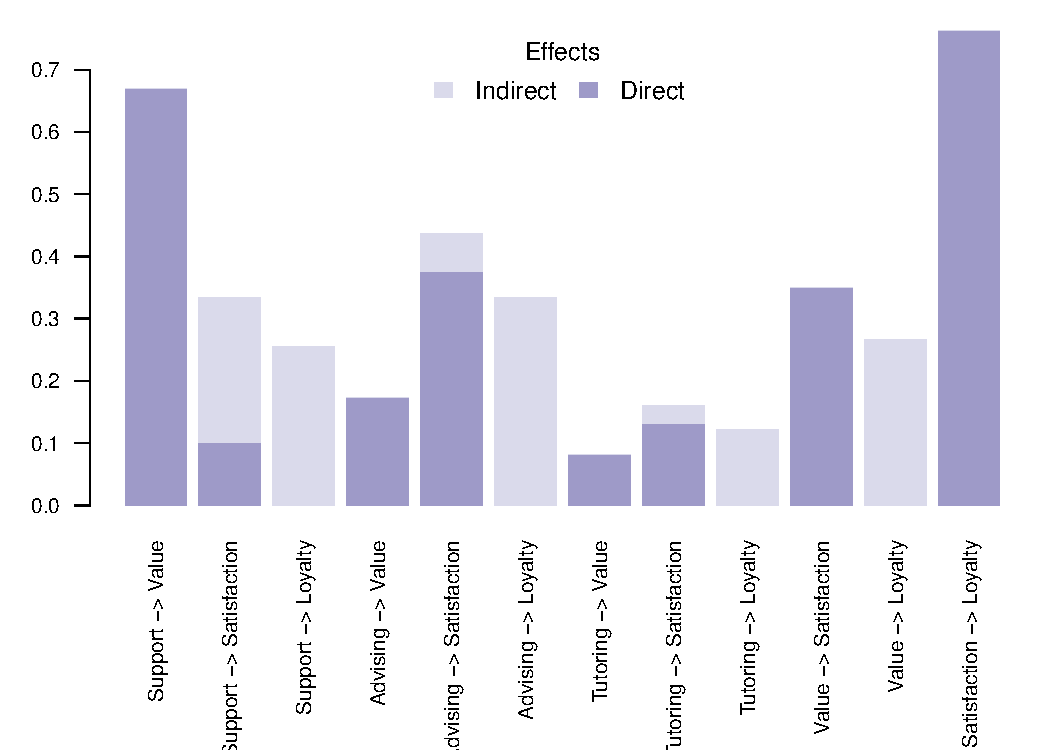
\includegraphics[width=1\linewidth,height=.7\linewidth]{figure/edu_pls3_effects_barchart} 

}

\caption[Total Effects]{Total Effects: Direct + Indirect paths\label{fig:edu_pls3_effects_barchart}}
\end{figure}


\end{knitrout}


Once we have our matrix with path effects, we can create the bar chart like so:
\begin{knitrout}
\definecolor{shadecolor}{rgb}{0.969, 0.969, 0.969}\color{fgcolor}\begin{kframe}
\begin{alltt}
\hlcomment{# setting margin size}
op = \hlfunctioncall{par}(mar = \hlfunctioncall{c}(8, 3, 1, 0.5))
\hlcomment{# barplots of total effects (direct + indirect)}
\hlfunctioncall{barplot}(\hlfunctioncall{t}(path_effs), border = NA, col = \hlfunctioncall{c}(\hlstring{"#9E9AC8"}, \hlstring{"#DADAEB"}),
        las = 2, cex.names = 0.8, cex.axis = 0.8, 
        legend = \hlfunctioncall{c}(\hlstring{"Direct"}, \hlstring{"Indirect"}),        
        args.legend = \hlfunctioncall{list}(x = \hlstring{"top"}, ncol = 2, border = NA, 
                           bty = \hlstring{"n"}, title = \hlstring{"Effects"}))
\hlcomment{# resetting default margins}
\hlfunctioncall{par}(op)
\end{alltt}
\end{kframe}
\end{knitrout}

The first line defines the graphical parameter \code{mar} that sets the figure margins to the specfied values. Then we have the function \code{barplot()}. Note that we are using \code{t(path\_effs)} which means that we are trasposing the matrix of path effects. To get nice bars I avoid borders (\code{border=NA}). The vector of colors \code{col} is expressed in \textit{hexadecimal} (hex) notation. Then we have another graphical parameter \code{las=2} that is used to specify the style of the axis labels in a perpendicular way, making numbers easier to read and showing the x-axis labels in vertical way. The \code{cex} arguments indicate the expansion of the names and axis-numbers. \code{legend} is a character vector with the labels used for the displayed legend. And finally, there is a long list of parameters in \code{args.legend} that are passed to the function \code{legend()}. Your homework is to use \code{help(legend)} to see the meaning behind the arguments in \code{args.legend}.



\subsection{Inner Model Summary}
The next set of results that you need to evaluate are the summary indices contained in \code{\$inner\_summary}. This is a data frame with diferent metrics that provides you with an overall summary of the structural model. 
\begin{knitrout}
\definecolor{shadecolor}{rgb}{0.969, 0.969, 0.969}\color{fgcolor}\begin{kframe}
\begin{alltt}
edu_pls3$inner_summary
\end{alltt}
\begin{verbatim}
##                    Type     R2 Block_Communality Mean_Redundancy
## Support       Exogenous 0.0000            0.6528          0.0000
## Advising      Exogenous 0.0000            0.8238          0.0000
## Tutoring      Exogenous 0.0000            0.6974          0.0000
## Value        Endogenous 0.6612            0.7878          0.5209
## Satisfaction Endogenous 0.6247            0.8368          0.5227
## Loyalty      Endogenous 0.5837            0.7655          0.4468
##                 AVE
## Support      0.6528
## Advising     0.8238
## Tutoring     0.6974
## Value        0.7878
## Satisfaction 0.8368
## Loyalty      0.7655
\end{verbatim}
\end{kframe}
\end{knitrout}


We already saw the \code{R2} values when we inspected the structural regressions, so let's focus on the last three columns. The average communality \texttt{Av.Commu} indicates how much of a reflective block variability is reproducible by the latent variable. On average, we would expect to have at least 50\% of communality in a reflective block. The next column \texttt{Av.Redun} is the average redundancy which reflects the ability of the independent latent variables to explain the average variation of the indicators in the dependent latent variable. For isntance, the average redundancy for \code{Loyalty} implies that \code{Satisfaction} predicts 44\% of the variability in \code{Loyalty} indicators.

The last columnn \code{AVE} is the \textit{Average Variance Extracted} which measures the amount of variance that a latent variable captures from its indicators in relation to the amount of variance due to measurement error. As a rule of thumb, we should check that AVE is greater than 0.50 which means that 50\% or more of the indicators's variance is accounted for.


\subsection{GoF}
The final measure of quality that we need to examine is the so-called GoF index contained in \code{\$gof}. This is a pseudo Goodness-of-Fit measure that attempts to account for the overall quality at both the measurement and the structural models. Basically, GoF assess the overall prediction performance of the model by taking into account the communality and the $R^2$ coefficients. However, you can also use the GoF index in presence of formative blocks, in which case more importance will be given to the average R2.
\begin{knitrout}
\definecolor{shadecolor}{rgb}{0.969, 0.969, 0.969}\color{fgcolor}\begin{kframe}
\begin{alltt}
\hlcomment{# gof index}
edu_pls3$gof
\end{alltt}
\begin{verbatim}
## [1] 0.6891
\end{verbatim}
\end{kframe}
\end{knitrout}


You can think of GoF as an index of average prediction for the entire model. Although this is not entirely exact, it helps to understand GoF values. From this point of view, a GoF value of 0.689 could be roughly interpreted as if the prediction power of the model is of 69\%. The naive rule of thumb is: the higher, the better. GoF values greater than 0.7 are considered as ``very good'' within the PLS-PM community.



\subsection{Bootstrap Validation}
Since PLS-PM does not rest on any distributional assumptions, resampling procedures are used to obtain information about the variability of the parameter estimates. \fplspm{} provides bootstrap resampling to get confidence intervals for evaluating the precision of the PLS parameter estimates. 
So far we haven't required bootstrap validation because we needed to check first that the results of the outer and inner models make sense. But now that we are satisfied with the obtained results, we can proceed with the bootstrap validation. We use the argument \code{boot.val = TRUE} to indicate that we wish to perform bootstrap validation. By default \fplspm{} runs 100 resamples but we can specify a different number. For instance, let's get a validation with \code{br=200} resamples:
\begin{knitrout}
\definecolor{shadecolor}{rgb}{0.969, 0.969, 0.969}\color{fgcolor}\begin{kframe}
\begin{alltt}
\hlcomment{# running bootstrap validation}
edu_val = \hlfunctioncall{plspm}(education, edu_path, edu_blocks3, modes = edu_modes, 
    boot.val = TRUE, br = 200)

\hlcomment{# bootstrap results}
edu_val$boot
\end{alltt}
\begin{verbatim}
## $weights
##           Original Mean.Boot Std.Error perc.025 perc.975
## sup.help    0.4571    0.4570  0.022206   0.4143   0.4963
## sup.safe    0.3747    0.3755  0.033703   0.3165   0.4539
## sup.conc    0.4021    0.4024  0.026926   0.3506   0.4531
## adv.comp    0.2652    0.2659  0.014300   0.2371   0.2896
## adv.acces   0.2572    0.2583  0.018846   0.2263   0.2980
## adv.comm    0.2879    0.2891  0.017785   0.2573   0.3291
## adv.qual    0.2903    0.2910  0.012223   0.2705   0.3154
## tut.prof    0.3024    0.3070  0.030564   0.2641   0.3815
## tut.sched   0.3154    0.3203  0.028988   0.2712   0.3792
## tut.stud    0.2974    0.2989  0.025552   0.2426   0.3475
## tut.qual    0.2830    0.2756  0.027963   0.2166   0.3202
## val.devel   0.2637    0.2626  0.009782   0.2443   0.2821
## val.deci    0.2764    0.2766  0.010163   0.2582   0.2985
## val.meet    0.2743    0.2747  0.009834   0.2578   0.2937
## val.info    0.3137    0.3157  0.016386   0.2888   0.3485
## sat.glad    0.3579    0.3578  0.010763   0.3400   0.3795
## sat.expe    0.3543    0.3574  0.014224   0.3353   0.3870
## sat.over    0.3807    0.3839  0.017428   0.3596   0.4236
## loy.proud   0.3874    0.3945  0.035610   0.3410   0.4709
## loy.recom   0.4082    0.4095  0.021787   0.3710   0.4606
## loy.back    0.3447    0.3442  0.029452   0.2865   0.3975
## 
## $loadings
##           Original Mean.Boot Std.Error perc.025 perc.975
## sup.help    0.8697    0.8684   0.02501   0.8039   0.9120
## sup.safe    0.7631    0.7622   0.04362   0.6650   0.8381
## sup.conc    0.7872    0.7846   0.03881   0.6977   0.8457
## adv.comp    0.9061    0.9014   0.02344   0.8529   0.9386
## adv.acces   0.8565    0.8521   0.03415   0.7743   0.9074
## adv.comm    0.9165    0.9140   0.02030   0.8647   0.9481
## adv.qual    0.9491    0.9472   0.01290   0.9225   0.9671
## tut.prof    0.8772    0.8752   0.02082   0.8260   0.9094
## tut.sched   0.8466    0.8439   0.02518   0.7956   0.8845
## tut.stud    0.7746    0.7728   0.05030   0.6589   0.8606
## tut.qual    0.8388    0.8291   0.05134   0.7177   0.9110
## val.devel   0.8956    0.8942   0.01819   0.8564   0.9288
## val.deci    0.8893    0.8888   0.02043   0.8421   0.9234
## val.meet    0.9044    0.9034   0.01693   0.8706   0.9329
## val.info    0.8604    0.8597   0.02073   0.8203   0.8998
## sat.glad    0.9053    0.8977   0.03380   0.8125   0.9442
## sat.expe    0.9125    0.9100   0.02104   0.8622   0.9420
## sat.over    0.9264    0.9218   0.01913   0.8817   0.9544
## loy.proud   0.8873    0.8860   0.02358   0.8356   0.9241
## loy.recom   0.9246    0.9177   0.02601   0.8666   0.9570
## loy.back    0.8089    0.7959   0.05779   0.6573   0.8814
## 
## $paths
##                          Original Mean.Boot Std.Error perc.025 perc.975
## Support -> Value          0.67021   0.67403   0.04855  0.57052   0.7604
## Support -> Satisfaction   0.10043   0.09974   0.08666 -0.06921   0.2600
## Advising -> Value         0.17273   0.16836   0.05041  0.08012   0.2627
## Advising -> Satisfaction  0.37640   0.37441   0.08251  0.21433   0.5201
## Tutoring -> Value         0.08196   0.07759   0.05265 -0.02599   0.1757
## Tutoring -> Satisfaction  0.13121   0.12970   0.05982  0.02232   0.2428
## Value -> Satisfaction     0.34927   0.34497   0.09323  0.17300   0.5427
## Satisfaction -> Loyalty   0.76398   0.74742   0.06847  0.59284   0.8543
## 
## $rsq
##              Original Mean.Boot Std.Error perc.025 perc.975
## Value          0.6612    0.6632   0.04967   0.5557   0.7425
## Satisfaction   0.6247    0.6216   0.07062   0.4968   0.7412
## Loyalty        0.5837    0.5633   0.09815   0.3515   0.7299
## 
## $total.efs
##                          Original Mean.Boot Std.Error perc.025 perc.975
## Support -> Advising       0.00000   0.00000   0.00000  0.00000   0.0000
## Support -> Tutoring       0.00000   0.00000   0.00000  0.00000   0.0000
## Support -> Value          0.67021   0.67403   0.04855  0.57052   0.7604
## Support -> Satisfaction   0.33452   0.33243   0.06847  0.19932   0.4615
## Support -> Loyalty        0.25557   0.24796   0.05342  0.14299   0.3467
## Advising -> Tutoring      0.00000   0.00000   0.00000  0.00000   0.0000
## Advising -> Value         0.17273   0.16836   0.05041  0.08012   0.2627
## Advising -> Satisfaction  0.43673   0.43203   0.08366  0.26294   0.6008
## Advising -> Loyalty       0.33365   0.32495   0.07749  0.17384   0.4800
## Tutoring -> Value         0.08196   0.07759   0.05265 -0.02599   0.1757
## Tutoring -> Satisfaction  0.15983   0.15620   0.05943  0.04578   0.2587
## Tutoring -> Loyalty       0.12211   0.11691   0.04553  0.03392   0.1926
## Value -> Satisfaction     0.34927   0.34497   0.09323  0.17300   0.5427
## Value -> Loyalty          0.26683   0.25783   0.07334  0.13017   0.3950
## Satisfaction -> Loyalty   0.76398   0.74742   0.06847  0.59284   0.8543
\end{verbatim}
\end{kframe}
\end{knitrout}

We obtain bootstrapped results for the outer weights, the loadings, tha path coefficients, the $R^2$ and the total effects. For each of the displayed results, we should examine the bootstrap confidence interval (95\%) provided by the percentiles 0.025 and 0.975. This is specially important for the path coefficients:
\begin{knitrout}
\definecolor{shadecolor}{rgb}{0.969, 0.969, 0.969}\color{fgcolor}\begin{kframe}
\begin{alltt}
\hlcomment{# bootstrap path coefficients}
edu_val$boot$paths
\end{alltt}
\begin{verbatim}
##                          Original Mean.Boot Std.Error perc.025 perc.975
## Support -> Value          0.67021   0.67403   0.04855  0.57052   0.7604
## Support -> Satisfaction   0.10043   0.09974   0.08666 -0.06921   0.2600
## Advising -> Value         0.17273   0.16836   0.05041  0.08012   0.2627
## Advising -> Satisfaction  0.37640   0.37441   0.08251  0.21433   0.5201
## Tutoring -> Value         0.08196   0.07759   0.05265 -0.02599   0.1757
## Tutoring -> Satisfaction  0.13121   0.12970   0.05982  0.02232   0.2428
## Value -> Satisfaction     0.34927   0.34497   0.09323  0.17300   0.5427
## Satisfaction -> Loyalty   0.76398   0.74742   0.06847  0.59284   0.8543
\end{verbatim}
\end{kframe}
\end{knitrout}

As you can see from the previous table, bootstrap intervals for the path coefficients of \code{Support} on \code{Satisfaction} and \code{Tutoring} on \code{Value} contain the zero. Hence we may say that these coefficients are not significant at a 5\% confidence level.


\subsection{Inspecting scores of latent variables}
After checking the overall quality of the inner model and the prediction capacity, it is also interesting to inspect the obtained scores of the latent variables. The values in \code{\$scores} are standardized scores (mean zero, unit variance), thus if we use \code{summary()} we won't get much information:
\begin{knitrout}
\definecolor{shadecolor}{rgb}{0.969, 0.969, 0.969}\color{fgcolor}\begin{kframe}
\begin{alltt}
\hlcomment{# summary of latent variable scores}
\hlfunctioncall{summary}(edu_pls3$scores)
\end{alltt}
\begin{verbatim}
##     Support          Advising         Tutoring          Value       
##  Min.   :-3.148   Min.   :-5.766   Min.   :-4.090   Min.   :-3.781  
##  1st Qu.:-0.654   1st Qu.:-0.344   1st Qu.:-0.720   1st Qu.:-0.630  
##  Median : 0.164   Median : 0.269   Median : 0.279   Median : 0.227  
##  Mean   : 0.000   Mean   : 0.000   Mean   : 0.000   Mean   : 0.000  
##  3rd Qu.: 0.760   3rd Qu.: 0.792   3rd Qu.: 0.824   3rd Qu.: 0.890  
##  Max.   : 1.242   Max.   : 0.792   Max.   : 1.404   Max.   : 1.085  
##   Satisfaction       Loyalty      
##  Min.   :-6.644   Min.   :-6.493  
##  1st Qu.:-0.451   1st Qu.:-0.247  
##  Median : 0.323   Median : 0.576  
##  Mean   : 0.000   Mean   : 0.000  
##  3rd Qu.: 0.665   3rd Qu.: 0.576  
##  Max.   : 0.665   Max.   : 0.576
\end{verbatim}
\end{kframe}
\end{knitrout}



Instead of the \code{summary()} we can use a more informative alternative by plotting histograms of each latent variable with the \code{hist} function:
\begin{knitrout}
\definecolor{shadecolor}{rgb}{0.969, 0.969, 0.969}\color{fgcolor}\begin{figure}[h]


{\centering 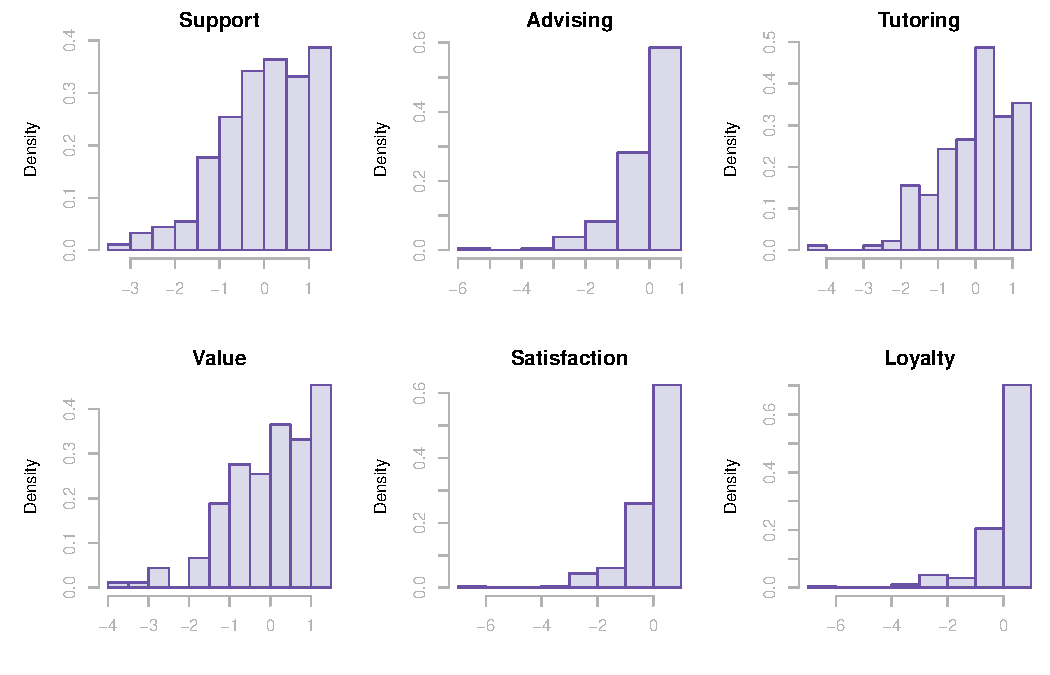
\includegraphics[width=0.95\linewidth,height=0.65\linewidth]{figure/edu_scores_histograms1} 

}

\caption[Histograms (in densities) of scores]{Histograms (in densities) of scores\label{fig:edu_scores_histograms1}}
\end{figure}


\end{knitrout}


This is the code to obtain the histograms in the figure above:
\begin{knitrout}
\definecolor{shadecolor}{rgb}{0.969, 0.969, 0.969}\color{fgcolor}\begin{kframe}
\begin{alltt}
\hlcomment{# setting graphic layout and margin sizes}
op = \hlfunctioncall{par}(mfrow = \hlfunctioncall{c}(2, 3), mar = \hlfunctioncall{c}(4, 5, 2, 0.5))
\hlcomment{# for each score}
\hlfunctioncall{for} (j in 1:6) \{
\hlcomment{    # histogram (with probability density)}
    \hlfunctioncall{hist}(edu_pls3$scores[, j], freq = FALSE, xlab = \hlstring{""}, border = \hlstring{"#6A51A3"}, 
        col = \hlstring{"#DADAEB"}, main = \hlfunctioncall{colnames}(edu_pls3$scores)[j])
\hlcomment{    # add axes}
    \hlfunctioncall{axis}(side = 1, col = \hlstring{"gray70"}, col.axis = \hlstring{"gray70"})
    \hlfunctioncall{axis}(side = 2, col = \hlstring{"gray70"}, col.axis = \hlstring{"gray70"})
\}
\hlfunctioncall{par}(op)
\end{alltt}
\end{kframe}
\end{knitrout}


\subsubsection*{Rescaling Scores}
Because all the manifest variables in \code{education} are expressed in the same scale (from 1 to 7), it would be interesting and convenient to have the scores of the latent variables expressed in the same scale as the indicators. This can be done by normalizing the outer weights in each block of indicators so that the weights are expressed as proportions. However, in order to apply this normalization all the outer weights must be positive.

You can apply the function \code{rescale()} to the object \code{edu\_pls3} and get scores expressed in the original scale of the manifest variables. Once you get the rescaled scores you can use \code{summary()} to verify that the obtained results make sense (i.e. scores expressed in original scale of indicators):
\begin{knitrout}
\definecolor{shadecolor}{rgb}{0.969, 0.969, 0.969}\color{fgcolor}\begin{kframe}
\begin{alltt}
\hlcomment{# rescaling scores}
Scores = \hlfunctioncall{rescale}(edu_pls3)

\hlcomment{# summary}
\hlfunctioncall{summary}(Scores)
\end{alltt}
\begin{verbatim}
##     Support        Advising       Tutoring        Value     
##  Min.   :1.61   Min.   :1.23   Min.   :1.77   Min.   :1.28  
##  1st Qu.:4.67   1st Qu.:6.00   1st Qu.:5.00   1st Qu.:5.00  
##  Median :5.65   Median :6.53   Median :5.98   Median :6.00  
##  Mean   :5.47   Mean   :6.30   Mean   :5.67   Mean   :5.71  
##  3rd Qu.:6.37   3rd Qu.:7.00   3rd Qu.:6.48   3rd Qu.:6.76  
##  Max.   :7.00   Max.   :7.00   Max.   :7.00   Max.   :7.00  
##   Satisfaction     Loyalty    
##  Min.   :1.00   Min.   :1.00  
##  1st Qu.:6.00   1st Qu.:6.34  
##  Median :6.68   Median :7.00  
##  Mean   :6.44   Mean   :6.51  
##  3rd Qu.:7.00   3rd Qu.:7.00  
##  Max.   :7.00   Max.   :7.00
\end{verbatim}
\end{kframe}
\end{knitrout}


With the rescaled \code{Scores} we can create another graphic with histograms to see the distributions of the latent variables in a more meaningful way:
\begin{knitrout}
\definecolor{shadecolor}{rgb}{0.969, 0.969, 0.969}\color{fgcolor}\begin{kframe}
\begin{alltt}
\hlcomment{# setting graphic layout and margin sizes}
op = \hlfunctioncall{par}(mfrow = \hlfunctioncall{c}(2,3), mar = \hlfunctioncall{c}(4, 5, 2, 1.5), bty = \hlstring{"n"})

\hlcomment{# for each score}
\hlfunctioncall{for} (j in 1:6)
\{
\hlcomment{  # histogram (not showing axes)}
  \hlfunctioncall{hist}(Scores[,j], main = \hlfunctioncall{colnames}(Scores)[j], axes = FALSE, 
       xlim = \hlfunctioncall{c}(1,7), ylim = \hlfunctioncall{c}(0, 125), xlab = \hlstring{""}, 
       border = \hlstring{"#6A51A3"}, col = \hlstring{"#DADAEB"})
\hlcomment{  # add horizontal axis}
  \hlfunctioncall{axis}(side = 1, col = \hlstring{"gray70"}, col.axis = \hlstring{"gray70"})
\hlcomment{  # add vertical axis}
  \hlfunctioncall{axis}(side = 2, col = \hlstring{"gray70"}, col.axis = \hlstring{"gray70"}, las = 2)
\}

\hlcomment{# resetting default graphical parameters}
\hlfunctioncall{par}(op)
\end{alltt}
\end{kframe}
\end{knitrout}


\begin{knitrout}
\definecolor{shadecolor}{rgb}{0.969, 0.969, 0.969}\color{fgcolor}\begin{figure}[h]


{\centering 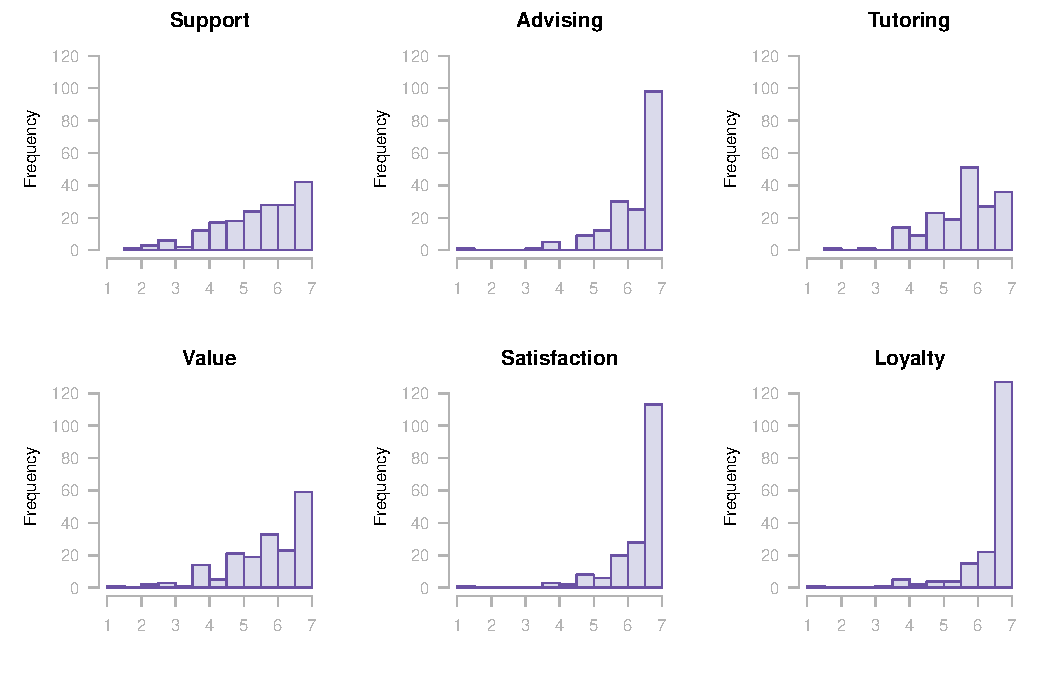
\includegraphics[width=0.95\linewidth,height=0.65\linewidth]{figure/edu_scores_histograms2} 

}

\caption[Histograms of rescaled scores]{Histograms of rescaled scores\label{fig:edu_scores_histograms2}}
\end{figure}


\end{knitrout}


Another graphical tool that we can apply is to get scatter plots with the function \code{pairs()}
\begin{knitrout}
\definecolor{shadecolor}{rgb}{0.969, 0.969, 0.969}\color{fgcolor}\begin{kframe}
\begin{alltt}
\hlcomment{# scatter plots of rescaled scores}
\hlfunctioncall{pairs}(Scores, pch = 19, cex = 0.7, col = \hlstring{"#807DBA33"}, cex.axis = 0.8, 
      col.axis = \hlstring{"gray70"}, gap = 0.5)
\end{alltt}
\end{kframe}\begin{figure}[h]


{\centering 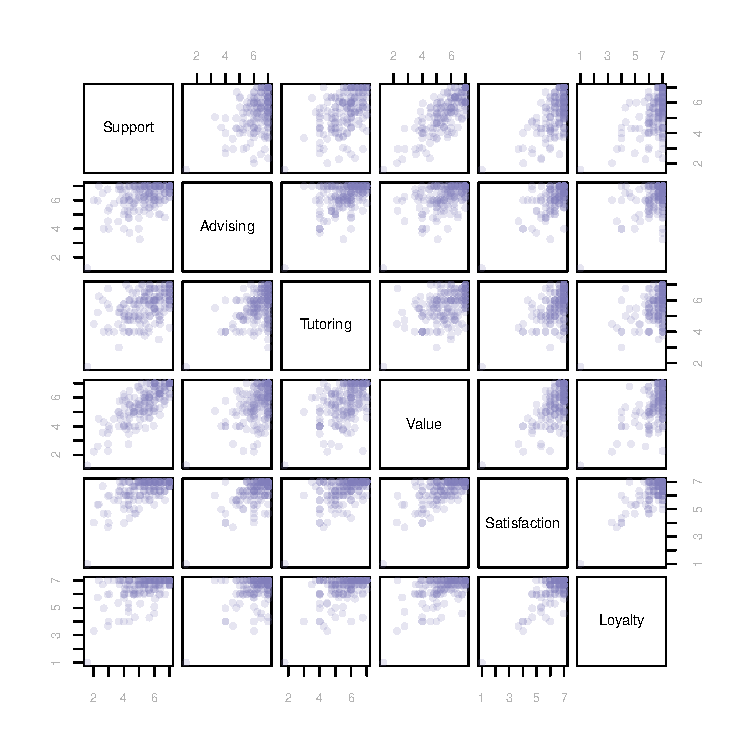
\includegraphics[width=0.9\linewidth,height=0.9\linewidth]{figure/edu_scores_pairs} 

}

\caption[Scatter plots of latent variable scores]{Scatter plots of latent variable scores\label{fig:edu_scores_pairs}}
\end{figure}


\end{knitrout}





\section{Guidelines for a PLS-PM analysis}
We'll end this chapter by providing some general guidelines and advices for performing PLS Path Modeling analysis. 

\paragraph{Urban Legend}
First we need to address one important issue that you will often find about why to use PLS-PM:
``because it makes no sample size assumptions and you can even use it with small sample sizes''. This is one of the not-so-accurate claims that many people make about PLS-PM. Although it is true that PLS-PM does not impose sample size restrictions, this does not mean that you can abuse by applying it with ridiculously small sample sizes. 

\paragraph{Rule of thumb}
The only thing for sure we can say is that there is no rule of thumb about a minimum number of observations that can be applied to all situations. In fact, how large or small the sample size should be is something that depends on various factors: the strength of the relationships between the variables, the complexity of the model, the proportion of missing values, and even the distribution of the observed variables.

In the article \textit{The Partial Least Squares Approach to Structural Equation Modeling}, Wynne Chin (1998) provides some recommendations:
\begin{quotation} \noindent
``If one were to use a regression heuristic of 10 cases per indicator, the sample size requirement would be 10 times either: a) the block with the largest number of indicators; or b) the largest structural equation''
\end{quotation}

In another publication, \textit{Structural Equation Modeling Analysis with Small Samples Using Partial Least Squares}, Wynne Chin and Peter Newsted (1999) make it clear that for the sample size for PLS path models to be determined, requires ``a power analysis based on the portion of the model with the largest number of predictors''.

\paragraph{Consistency at Large}
The concept that we should keep in mind is the so-called \textit{consistency at large} which basically means:
\begin{itemize}
 \item The larger the sample size, the better: PLS estimates improve as sample size increases; and their average absolute error rates diminish .
 \item The more indicators per latent variable, and the larger the number of observations, the better PLS estimates you'll get.
\end{itemize}




\subsection*{Some Personal Tips and Advices}

\paragraph{\#1 Get to know your data}
Seriously. Spend as much time as possible ``chatting'' with your data. Above all: visualize it! Do barplots, scatter plots, histograms, glyphs, PCA plots, dendrograms, you name it. Also, get summary statistics, measures of dispersion. I can hardly stress out all the positive effects that you can achieve by getting to know your data, but be assured that they are enormous.

\paragraph{\#2 Talk to the ``experts''}
By experts I mean the people running the business of your data, either those who designed the survey, those who you are consulting for, or those who have the \textit{big picture} of the field you are working in. Maybe you are the expert. In that case, go and talk to other experts, ask for a second opinion of what you are doing; whether your model and its underlying hypotheses make sense.

\paragraph{\#3 Read papers}
See what other people are doing; how do they draw the diagrams, what jargon and argot they use, how do they report the results, etc. Get inspired and steal like an artist (but don't plagiarize, please).

\paragraph{\#4 Learn to lose}
Face it: sometimes the data in your hands does not cooperate with you. Maybe the data is simply crap or maybe is not suited for PLS-PM. The worst you can do is forcing fitting a model. I've tried to force models, sometimes working-around and finding a non-trivial solution. But most of the times I will eventually realize that there is nothing I can do. This is specially the case when somebody has a dataset and wants stubbornly to do something with it. Perhaps a researcher wants to publish a paper or prepare a talk, and they will ask you to do some magic with PLS-PM (or any other method). That's the time when you have to learn to say no.

\paragraph{\#5 Be cautious}
Specially when you are mixing very different types of data. For instance, you may have observational data like macroeconomic indices or demographic statistics, and then you also have perception data. It's like trying to mix oil and water: economic indices with poeple's thoughts. That's a combination that you need to handle with tweezers, specially when drawing any type of conclusion. I'm not saying that you shouldn't do it, I'm just saying be cautious.

\paragraph{\#6 Practice, practice, practice}
As with any other skill that you want to master (like a sport, hobby, language, etc) you need to practice as much as possible to be a PLS \textit{ninja}. I don't have a recipe for you that allows you to \textit{learn PLS-PM in 30 minutes} or something like that. My best advice is to practice, and if possible, get to work under the guidance of a PLS-PM guru.


\section{Reading List}
\paragraph{ECSI Model in Education} 
Some papers with applications of PLS Path Modeling to Education:
\begin{itemize}
 \vspace{2mm}
 \item \textbf{\textsf{The Influence of University Image in Student's Expectations, Satisfaction and Loyalty}} by Helena Alves and Mario Reposado (2007). Paper presented at the 29th Annual EAIR Forum (Innbrusck, Austria).

 \vspace{2mm}
 \item \textbf{\textsf{Measuring Student Oriented Quality in Higher Education: Application of the ECSI Methodology}} by Anne Martensen, Lars Gronholdt, Jacob K. Eskildsen and Kai Kristensen (1999). Paper presented at the conference \textit{TQM for Higher Education Institutions II} (Universita di Verona, Italy)

 \vspace{2mm}
 \item \textbf{\textsf{Drivers of student satisfaction and loyalty at different levels of higher education (HE) -cross-institutional results based on ECSI methodology}} by Dean Peder Ostergaard and Kai Kristensen (2005). Paper presented at the Society for Research into Higher Education (SRHE) Available at: \\
 \texttt{\href{http://pure.au.dk/portal/files/214/PAPER\_SRHE\_2005\_SESSION\_PAPER\_6.31.PDF}{http://pure.au.dk/portal/files/214/PAPER\_SRHE\_2005\_SESSION\_PAPER\_6.31.PDF}}

 \vspace{2mm}
 \item \textbf{\textsf{Is the European Customer Satisfaction Index Model Applicable to Tertiary Education?}} by Bill Chitty and Geoffrey N. Soutar (2004). Paper presented at the Australian and New Zealand Marketing Academy (ANZMAC). Available at: \\
 \texttt{\href{http://anzmac.info/conference/2004/papers/Chitty1.PDF}{http://anzmac.info/conference/2004/papers/Chitty1.PDF}}

 \vspace{2mm}
 \item \textbf{\textsf{Evaluating the quality of the university educational process: an application of the ECSI model}} by Bruno Chiandotto, Matilde Bini and Bruno Bertaccini. Available at: \\
 \texttt{\href{http://valmon.ds.unifi.it/docpub/ECSI\%20BCMBBB\_engversion.pdf}{http://valmon.ds.unifi.it/docpub/ECSI\%20BCMBBB\_engversion.pdf}}
\end{itemize}
  

\paragraph{PLS-PM analysis}
Other resources about PLS Path Modeling and how to carry out PLS-PM analysis:
\begin{itemize}
 \vspace{2mm}
 \item \textbf{\textsf{How to Write Up and Report PLS Analyses}} by Wynne Chin (2010). This is the Chapter 28 of the \textit{Handbook of Partial Least Squares}. This chapter describes the general steps to be performed for writing a report on results from a PLS-PM analysis.

 \vspace{2mm}
 \item \textbf{\textsf{Evaluation of Structural Equation Models Using Partial Least Squares (PLS) Approach}} by Oliver Gotz, Kerstin Liehr-Gobbers and Manfred Krafft (2010). As Chapter 29 of the \textit{Handbook of Partial Least Squares}, it provides a basic comprehension of PLS-PM and it discussess key guidelines for evaluation of structural models.

 \vspace{2mm}
 \item \textbf{\textsf{The Use of Partial Least Squares Path Modeling in International Marketing}} by Jorg Henseler, Christian Ringle and Rudolf R. Sinkovics (2009). This article in \textit{New Challenges to International Marketing Advances in International Marketing} (Vol. 20, 277 - 319) offers guidance for the use of PLS with an emphasis on reasearch studies on marketing research. Covers the requirements, strengths and weaknesses of PLS-PM.

 \vspace{2mm}
 \item \textbf{\textsf{The Partial Least Squares to Structural Equation Modeling}} by Wynne Chin (1998). As Chapter 10 of the book \textit{Modern Methods for Business Research} (George A. Marcoulides editor; pp: 295-336), this article is one of the classic references of Chin when he describes the PLS-PM methodology for a business research audience. 

\vspace{2mm}
 \item \textbf{\textsf{Structural Equation Modeling Analysis With Small Samples Using Partial Least Squares}} by Wynne Chin and Peter Newsted (1999). This article in Chapter 12 of the book \textit{Statistical Strategies for Small Sample Research} (Rick H. Hoyle editor; pp: 307-341), provides a comprehensive overview of PLS-PM for non-statisticians.

 \vspace{2mm}
 \item \textbf{\textsf{PLS: A Silver Bullet?}} by George A. Marcoulides and Carol Saunders (2006). This is an Editorial comment in the journal \textit{MIS Quarterly} (Vol. 30, No. 2). The authors express their concerns about claims made by a number of authors about taking PLS as a magic wand that can be applied indiscriminately to all problems.

 \vspace{2mm}
 \item \textbf{\textsf{A Critical Look at Partial Least Squares Modeling}} by George A. Marcoulides, Wynne W. Chin and Carol Saunders (2009). This is the Foreword in the Special Issue Section of the journal \textit{MIS Quarterly} (Vol. 33, No. 1, 171-175). The authors express their concerns about claims made by a number of authors about taking PLS as a magic wand that can be applied indiscriminately to all problems.
\end{itemize}
  


% Chapter6

% !Rnw root = ../PLS_Path_Modeling_with_R.Rnw


\chapter{Comparing Groups}
In the previous chapters we've been discussing a lot of information related to the basics of PLS Path Modeling. But now it's time to take it to the next level. In this and the following chapters, we are going to review some of the topics that cover a range of additional modeling tasks like group comparisons, higher-order constructs, moderating effects, and class detection. As we move forward, you may feel the need to reread parts of the material exposed in the earlier sections. That's totally fine and there's nothing to worry about that; PLS Path Modeling is not something you learn in a couple of days after reading one book. The present chapter is dedicated to \textit{multi-group comparison} or \textit{multiple group analysis}. To start moving into deep water we'll begin with the challenging question of how to compare groups in PLS-PM.


\section{The million dollar question}
Let's face it: often, estimating one single PLS path model is not enough. I'm not referring to 
play with one model under slightly different configurations. I'm talking about dealing with information from different groups in data. For instance, when we work with survey data it is almost inevitable to have demographic information like the gender or age of the respondants. When you have groups for females and males, you ask yourself about possible differences between the two genders. This is an issue that has to do with the comparison of path models which leads us to the fundamental question of: 
\begin{quote}
\textit{Given two structural models, how can they be compared?}
\end{quote}

Why is this question so important? Because given the complexity of path models in general, the truth is that there is no simple answer for it. In fact, path models may be different at so many levels that there are many ways in which they can be compared. Broadly speaking we have four major types of differences:

\begin{itemize}
 \item \textbf{Differences at the causal network level}: this refers to differences in the assumed causal-effect network linking the latent variables. Take for example the case of teenagers and adult consumers; while two latent variables may be positively correlated for teenagers, the same latent variables may be uncorrelated for adults. In other words, the two latent variables would be connected in the teenagers model but not in the model of adults.
 
 \item \textbf{Differences at the structural level}: this involves differences in magnitude of the structural coefficients (i.e. the path coefficients). For instance, there may be two groups of customers: in one group satisfaction is driven by the perceived value of the product they consume, whereas satisfaction in the other group is driven by the perceived quality.
 
 \item \textbf{Differences at the measurement level}: this refers to the way in which the latent variables are defined by their indicators. While one indicator may be appropriate for some construct in one model, the same indicator may not be appropriated in another model.
 
 \item \textbf{Differences at the latent variables level}: this implies that the mean value (or other distribution characteristic) of latent variables across models may be different. For example, the mean value of Satisfaction may vary across groups in terms of marital status (e.g, single, married, divorced, etc).
\end{itemize}

\vspace{2mm}
In principle, none of the above levels is better or worse than the others. You can legitimately ask whether two models are different at the latent variables' distribution level. For instance, let's say we have a model about perception of gay marriage in the USA based on survey data, and that we have information on the political affiliation of the respondants. We could calculate a model for democrats and another model for republicans, and then compare the differences among the latent variables of each model. We could also look into possible differences in the indicators used in each model. Maybe there is a manifest variable that, for whatever reason, is only applicable to democrats. However, given that the main attractive feature of path models is in the inner part with the estimation of path coefficients, the traditional approach to compare path models focuses on differences at the structural level.

It's not hard to understand why people put an emphasis on comparing models by taking into account differences only at the structural level. The rationale for focusing on the structural coefficients involves the goals in path modeling with latent variables: estimate the linear relationships among constructs. Hence, we pay attention to the differences in the magnitude of the cause-effect relationships among constructs.

Of course, this standpoint is not without its weak points. The main limitation is that the rest of potential differences (network level, measurement level, and construct distributions level) are practically ignored. By paying attention to only differences in path coefficients, the structural network has to be the same across groups, otherwise we would be comparing completely different models. Also, to have a fair comparison of path coefficients across groups, no differences at the measurement level should be desirable; implying that the indicators has to be the same among models. Finally, regarding the option of comparing models at the latent variables level is often relegated to subsequent analyses of a more exploratory and descriptive nature.



\section{Group Comparison Approaches}
For the sake of convenience and following the tradition within the PLS-PM framework, I'll give priority to group differences at the structural level. This implies focusing on the path coefficients, although most of what we say could be applied to other parameters (outer weights, loadings, R2, gof index). In addition, I will suppose that we have a categorical variable defining the groups. The default example would be having the categorical variable gender; but you could also have things like ethnic group, income level, education level, geographic region, culture, etc.

\subsubsection*{Multi-group analysis? Not really. Just bi-group analysis}
Even though comparing groups is also called as ``multi-group comparison'' or ``multiple group analysis'', the truth is that most of the time the analysis focuses on only two groups. Why? Because it's so much easier! Thus, in practice we should talk about bi-group analysis instead of multi-group analysis. This, of course, is not exactly what we want when our categorical variable has more than two categories. When this happens, the suggestion is to break down your analysis in groups of two. Say you have a variable Size with three categories \textit{small}, \textit{medium} and \textit{large}. To do a multigroup analysis considering all the three categories you would need to compare:
\begin{itemize}
 \item[] small -vs- medium and large
 \item[] medium -vs- small and large
 \item[] large -vs- small and medium
\end{itemize}


\subsubsection*{Two major approaches}
PLS Path Modeling approaches for comparing groups can be classified in two major categories: 1) resampling methods and 2) moderating effects.
\begin{itemize}
 \item \textbf{Resampling methods}, as the name implies, involve performing some type of resampling procedure to test the difference between groups. The most popular options are the \textit{bootstrap t-test} and the \textit{permutation procedure}. These approaches are discussed in this chapter.
 \item \textbf{Moderating effects} implies treating the group variable (e.g. gender) as a \textit{moderator variable} and then apply one of the techniques used for testing moderating effects. Since moderating effects are not limited to only categorical variables, this approach has its own dedicated chapter (see chapter 7).
\end{itemize}

The resampling methods of this chapter (bootstrapping and permutation) apply computing power to relax some of the conditions needed for traditional inference. However, the main notions of statistical inference remain the same so we can answer the fundamental question: ``What would happen if we applied this method many times?'' Using these methods we can get sampling distributions of statistics that show what would happen if we took many samples under the same conditions.


\subsection{Bootstrap t-test}
This resampling approach for comparing groups involves using a \textit{t}-test based on bootstrap resamples. The procedure consists of separating the data into groups and then running bootstrap samples with replacement for each group. Path coefficients are calculated in each resampling and the standard error estimates are treated in a parametric sense via a \textit{t}-test. Because we use a parametric \textit{t}-test as well as bootstrap resamples, this method is also referred to as a \textit{resampling parametric approach}. 

To illustrate the basic idea of the bootstrap $t$-test, suppose we have two groups $G_1$ and $G_2$ with sample sizes of $n_1$ and $n_2$, respectively. Let's imagine that we want to compare a given path coefficient between both groups: $\beta_{ji}^{G_1}$ against $\beta_{ji}^{G_2}$. The question is: Are the path coefficients similarly enough to be considered the same? To find out whether the path coefficients are similar we do the following:

\begin{enumerate}
 \item Calculate a PLS path model for each group to obtain path coefficients $\beta_{ji}^{G_1}$ and $\beta_{ji}^{G_2}$.
 \item Separate the data into groups and run bootstrap samples for each group.
 \item For each sample, calculate a PLS path model to obtain resampling path coefficients.
 \item After running all the resamples (say 200 times), calculate the standard error estimates.
 \item Use the standard error estimates in a parametric sense via a $t$-test.
\end{enumerate}

\vspace{2mm}
The formula that we use for the $t$-test statistic is:
$$ t = \frac{Path_{ji}^{G_1} - Path_{ji}^{G_2}}
{\left( \sqrt{\frac{1}{n_1}+\frac{1}{n_2}} \right) Sp}  $$
which follows a \textit{t}-distribution with $n_1 + n_2 - 2$ degrees of freedom

As you can see from the previous formula, there is a special term in the denominator: $Sp$; this is the estimator of the pooled variance and is obtained as follows:
$$ Sp = \sqrt{\frac{(n_1-1)^2}{(n_1 + n_2 - 2)} SE_{G_1}^2 + 
\frac{(n_2-1)^2}{(n_1 + n_2 - 2)} SE_{G_2}^2}  $$
where $SE_{G_1}$ and $SE_{G_2}$ are the bootstrap Standard Errors of each group.

Keep in mind that the bootstrap procedure still depends on the assumptions of a $t$-test which relies on two major conditions: normal distributed data and similar sample size of groups. It is true that $t$ procedures are useful in practice because they are robust. However, when the data have less symmetric distributions, and the size of the groups are very different, the application of the bootstrap $t$-test wil be limited. This is often the case when we have data like opinions from customer satisfaction studies in which the distribution of the variables are strongly skewed. Unless our samples are quite large, you can expect the performance of the test to be deficient.

 


\subsection{Permutation Procedure}
Another type of resampling approach is based on randomization or permutation procedures. Compared to bootstrap samples (which are drawn with replacement), permutation resamples are drawn without replacement. The basic premise of this kind of test is to use the assumption that it is possible that all of the groups are equivalent, and that every member of the group is the same before sampling began. From this, one can calculate a statistic and then observe the extent to which this statistic is special by seeing how likely it would be if the group assignments had been jumbled/mixed.

Again, to illustrate the basic idea of a permutation test, suppose we have two groups $G_1$ and $G_2$ with path coefficients $\beta_{ji}^{G_1}$ and $\beta_{ji}^{G_2}$, and sample sizes of $n_1$ and $n_2$, respectively. The permutation test is designed to determine whether the observed difference between the path coefficients is large enough to reject the null hypothesis $H_0$ that the two groups can be considered identical. The test proceeds as follows:

\begin{enumerate}
 \item First, we calculate the test statistic for the data. In our case the test statistic is the difference of path coefficients between the two groups.
 \item Then we combine the observations of groups $G_1$ and $G_2$ into a single large group.
 \item Next, the data are permuted (divided or rearranged) repeatedly in a manner consistent with the random assignment procedure. Each permutation implies:
 \begin{itemize}
  \item dividing data in two groups of size $n_1$ and $n_2$
  \item estimating the PLS models for each group
  \item calculating and recording the test statistic
  \item[] The set of calculated differences is the distribution of possible differences
under the null hypothesis that group label does not matter.
 \end{itemize}
 \item Then, we sort the recorded differences and we check if the original test statistic is contained within say the middle 95\% of the sorted values. If it does not, we reject the null hypothesis of identical groups at the 5\% significance level.
\end{enumerate}

The main attractive of the permutation procedure is that is a distribution-free test that requires no parametric assumptions. Among the advantages of permutation tests we have that: 1) they do not require specific population shapes such as Normality; 2) they apply to a variety of statistics, not just to statistics that have a simple distribution under the null hypothesis; 3) they can give very accurate P-values, regardless of the shape and size of the population (if enough permutations are used).



\subsection{Case Study: College GPA}
The case study for this chapter is based on data of college students (from a university in California, USA) with undergraduate degrees in life sciences majors. The dataset comes with the package \plspm{} under the name \code{college}. To load the data in your R session use the \code{data()} function:
\begin{knitrout}\small
\definecolor{shadecolor}{rgb}{0.969, 0.969, 0.969}\color{fgcolor}\begin{kframe}
\begin{alltt}
\hlcomment{# only if you haven't load plspm}
\hlfunctioncall{library}(plspm)

\hlcomment{# load data college}
\hlfunctioncall{data}(college)

\hlcomment{# what does the data look like}
\hlfunctioncall{head}(college, n = 5)
\end{alltt}
\begin{verbatim}
##   HS_GPA SAT_Verbal SAT_Math Biology1 Chemistry1 Math1 Physics1
## 1   4.18        650      630      4.0        4.0   4.0        4
## 2   4.15        600      770      3.0        4.0   4.0        3
## 3   4.65        460      590      4.0        3.7   4.0        4
## 4   4.12        490      630      3.7        4.0   3.7        3
## 5   4.54        540      680      3.0        2.7   3.7        3
##   Biology2 Chemistry2 Math2 Physics2 FinalGPA Gender
## 1      4.0          4   3.7      4.0    3.952   MALE
## 2      2.7          3   4.0      3.4    3.352   MALE
## 3      4.0          4   3.0      3.4    3.633   MALE
## 4      3.0          4   4.0      3.4    3.737 FEMALE
## 5      3.0          2   2.0      3.0    3.281 FEMALE
\end{verbatim}
\end{kframe}
\end{knitrout}


The following table gives the description of each variable:

\begin{table}[h]
 \caption{Description of variables in data \code{college}} 
 \centering
 \begin{tabular}{l l}
  \hline
  Variable & Description \\
  \hline
  \code{HS\_GPA} & High School GPA  \\
  \code{SAT\_Verbal} & Verbal SAT score \\
  \code{SAT\_Math} & Math SAT score \\
  \code{Biology1} & Introductory Biology \\
  \code{Chemistry1} & Introductory Chemistry \\
  \code{Math1} & Calculus 1 \\
  \code{Physics1} & Introductory Physics \\
  \code{Biology2} & Intermediate Biology \\
  \code{Chemistry2} & Intermediate Chemistry \\
  \code{Math2} & Calculus 2 \\
  \code{Physics2} & Intermediate Physics \\
  \code{FinalGPA} & Graduation GPA \\
  \code{Gender} & Gender \\
  \hline
 \end{tabular}
 \label{tab:college}
\end{table}

In addition to \code{head()}, we can also use the function \code{str()} to get a detailed description of the structure of the data:
\begin{knitrout}\small
\definecolor{shadecolor}{rgb}{0.969, 0.969, 0.969}\color{fgcolor}\begin{kframe}
\begin{alltt}
\hlcomment{# what's the structure?}
\hlfunctioncall{str}(college)
\end{alltt}
\begin{verbatim}
## 'data.frame':	352 obs. of  13 variables:
##  $ HS_GPA    : num  4.18 4.15 4.65 4.12 4.54 4.16 4.2 3.93 4.18 4.6 ...
##  $ SAT_Verbal: int  650 600 460 490 540 640 540 620 660 630 ...
##  $ SAT_Math  : int  630 770 590 630 680 640 690 640 720 800 ...
##  $ Biology1  : num  4 3 4 3.7 3 2.7 2 2.4 2.7 4 ...
##  $ Chemistry1: num  4 4 3.7 4 2.7 4 2 2 2.7 4 ...
##  $ Math1     : num  4 4 4 3.7 3.7 4 3 3.7 4 4 ...
##  $ Physics1  : num  4 3 4 3 3 3.7 2.4 3 2.4 4 ...
##  $ Biology2  : num  4 2.7 4 3 3 4 2 2.4 2 3.4 ...
##  $ Chemistry2: num  4 3 4 4 2 3.4 2 2.7 0 4 ...
##  $ Math2     : num  3.7 4 3 4 2 3.4 1.7 2.7 2 3.7 ...
##  $ Physics2  : num  4 3.4 3.4 3.4 3 3 2 2.7 2.4 3.7 ...
##  $ FinalGPA  : num  3.95 3.35 3.63 3.74 3.28 ...
##  $ Gender    : Factor w/ 2 levels "FEMALE","MALE": 2 2 2 1 1 1 1 2 2 1 ...
\end{verbatim}
\end{kframe}
\end{knitrout}

As you can see, \code{college} is a \code{data.frame} containing 352 observations and 13 variables. The function \code{str()} also displays the storage mode of each variable as well as the first ten values of each variable. This is useful when we want to not only take a quick glance at the data but also to know the kind of treatment R is giving to the variables. Notice that \code{Gender} is being treated as a \code{factor} (i.e. a categorical variable). This is the grouping variable that we will take into account to perform a group analysis: comparing the performance between female and male students.




\subsubsection*{Your high school performance predicts your college GPA?}
It is often said that your performance in high school will be one of the key factors affecting your performance in college. Particularly in the United States, the high school GPA (Grade Point Average) is taken as \textit{the} indicator of how well a student will do in college. When high school students apply to college, besides submitting their GPA they also need to submit the obtained scores in the SAT test (formerly called the \textit{Scholastic Assessment Test}). The SAT test is a standardized test for college admissions in the USA and is intended to assess a student's academic readiness for college. Before 2006, the SAT test was divided in a Math section and a Verbal section.

\subsubsection*{Toy Model}
We are going to play with a toy model based on a simple progressive sequence depicted in the diagram shown below. Basically, the premise behind the model is: ``how well a student does in college (Final GPA) is affected by how well she does in the intermediate and introductory courses, as well as how well prepared she was in high school''.
\begin{knitrout}
\definecolor{shadecolor}{rgb}{0.969, 0.969, 0.969}\color{fgcolor}\begin{figure}[h]


{\centering 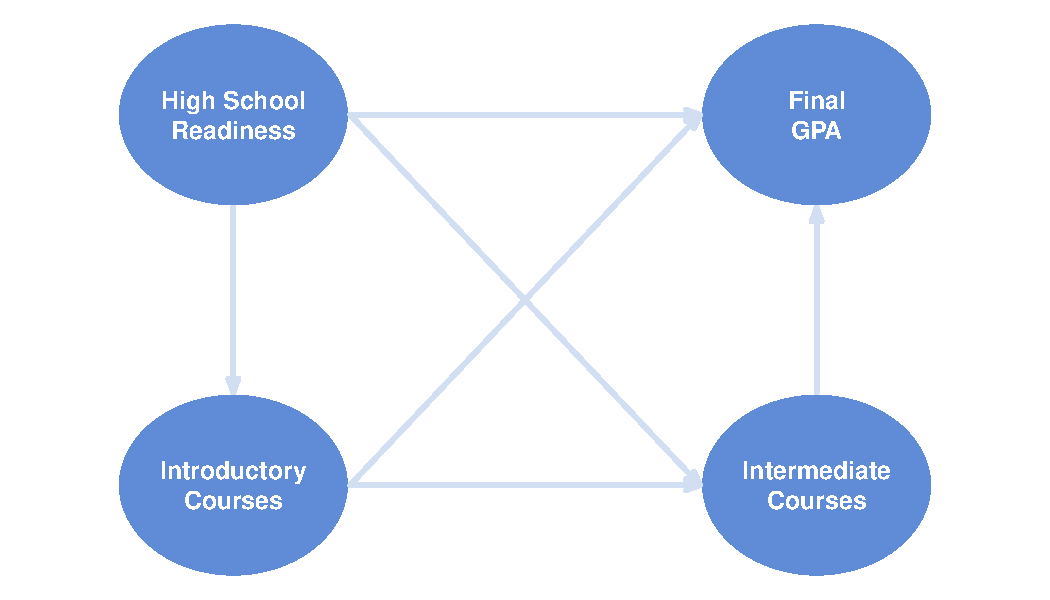
\includegraphics[width=.85\linewidth,height=.45\linewidth]{figure/gpa_dummy_model} 

}

\caption[College GPA Model]{College GPA Model\label{fig:gpa_dummy_model}}
\end{figure}


\end{knitrout}



\subsubsection*{Defining the complete path model}
The manifest variables in \code{college} can be grouped in four blocks as follows: 

\paragraph{High School Readiness}
\begin{itemize}
 \item[] High School GPA
 \item[] High School Math SAT Scores
 \item[] High School Verbal SAT Scores
\end{itemize}

\paragraph{Introductory Courses}
\begin{itemize}
 \item[] Biology 1: Evolution \& Ecology
 \item[] Chemistry 1: General Chemistry
 \item[] Physics 1: Introductory Physics I
 \item[] Math 1: Calculus I
\end{itemize}

\paragraph{Intermediate Courses}
\begin{itemize}
 \item[] Biology 2: Molecular \& Cell Biology
 \item[] Chemistry 2: Organic Chemistry 
 \item[] Physics 2: Introductory Physics II
 \item[] Math 2: Calculus II
\end{itemize}

\paragraph{Graduation}
\begin{itemize}
 \item[] Final GPA
\end{itemize}

\vspace{2mm}
The entire model is represented in the following path diagram:



\begin{knitrout}
\definecolor{shadecolor}{rgb}{0.969, 0.969, 0.969}\color{fgcolor}\begin{figure}[h]


{\centering 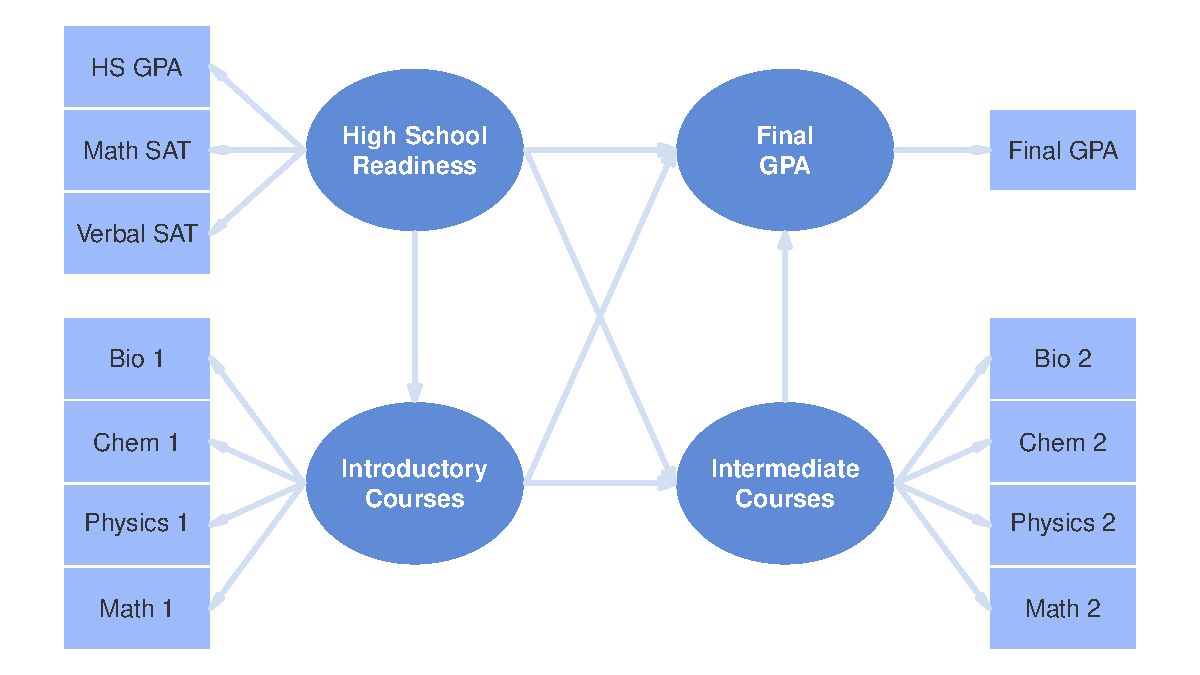
\includegraphics[width=.95\linewidth,height=.5\linewidth]{figure/gpa_model_diagram} 

}

\caption[College GPA Model]{College GPA Model\label{fig:gpa_model_diagram}}
\end{figure}


\end{knitrout}




\subsection{PLS-PM Analysis: GPA Model}
Let's start by performing a PLS-PM analysis on all 352 students. The first step is to define the required parameters for the \code{plspm()} function: the path model matrix, the list of \code{blocks} for the outer model, and the vector of modes.
\begin{knitrout}
\definecolor{shadecolor}{rgb}{0.969, 0.969, 0.969}\color{fgcolor}\begin{kframe}
\begin{alltt}
\hlcomment{# path matrix (inner model)}
HighSchool = \hlfunctioncall{c}(0, 0, 0, 0)
Intro = \hlfunctioncall{c}(1, 0, 0, 0)
Medium = \hlfunctioncall{c}(1, 1, 0, 0)
Graduation = \hlfunctioncall{c}(1, 1, 1, 0)
gpa_path = \hlfunctioncall{rbind}(HighSchool, Intro, Medium, Graduation)

\hlcomment{# list of blocks (outer model)}
gpa_blocks = \hlfunctioncall{list}(1:3, 4:7, 8:11, 12)

\hlcomment{# vector of reflective modes}
gpa_modes = \hlfunctioncall{rep}(\hlstring{"A"}, 4)
\end{alltt}
\end{kframe}
\end{knitrout}


Once we define the main ingredients, let's apply \fplspm{} asking for bootstrap validation with the argument \code{boot.val=TRUE}
\begin{knitrout}
\definecolor{shadecolor}{rgb}{0.969, 0.969, 0.969}\color{fgcolor}\begin{kframe}
\begin{alltt}
\hlcomment{# apply plspm}
gpa_pls = \hlfunctioncall{plspm}(college, gpa_path, gpa_blocks, modes = gpa_modes, 
                boot.val = TRUE)
\end{alltt}
\end{kframe}
\end{knitrout}


Let's see the results of the inner model
\begin{knitrout}
\definecolor{shadecolor}{rgb}{0.969, 0.969, 0.969}\color{fgcolor}\begin{kframe}
\begin{alltt}
\hlcomment{# plot path coefficients}
\hlfunctioncall{plot}(gpa_pls)
\end{alltt}
\end{kframe}\begin{figure}[h]


{\centering 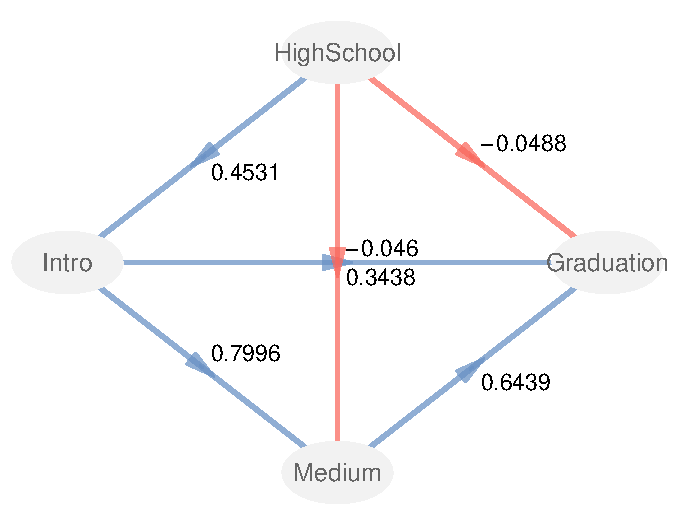
\includegraphics[width=.7\linewidth,height=.5\linewidth]{figure/gpa_inner_model} 

}

\caption[Inner model with path coefficients]{Inner model with path coefficients\label{fig:gpa_inner_model}}
\end{figure}


\end{knitrout}

As you can see from the path diagram, High School Readiness (\code{HighSchool}) has a positive effect on the Introductory courses (\code{Intro}) but it has a negative effect on the Intermediate courses (\code{Medium}) and on the Final GPA (\code{Graduation}). On the other hand, \code{Intro} has positive coefficients on both \code{Medium} and \code{Graduation}. In turn, \code{Medium} has also a positive effect on \code{Graduation}. To assess how relevant these results are we should check the bootstrapped path coefficients:
\begin{knitrout}
\definecolor{shadecolor}{rgb}{0.969, 0.969, 0.969}\color{fgcolor}\begin{kframe}
\begin{alltt}
\hlcomment{# bootstrapped path coefficients}
gpa_pls$boot$paths
\end{alltt}
\begin{verbatim}
##                          Original Mean.Boot Std.Error perc.025
## HighSchool -> Intro       0.45308   0.45556   0.04049  0.37493
## HighSchool -> Medium     -0.04603  -0.04227   0.03773 -0.10142
## HighSchool -> Graduation -0.04885  -0.04608   0.02178 -0.08753
## Intro -> Medium           0.79956   0.79903   0.02366  0.75674
## Intro -> Graduation       0.34382   0.34283   0.04325  0.23786
## Medium -> Graduation      0.64385   0.64371   0.03805  0.57361
##                           perc.975
## HighSchool -> Intro       0.529409
## HighSchool -> Medium      0.035321
## HighSchool -> Graduation -0.008007
## Intro -> Medium           0.842004
## Intro -> Graduation       0.411008
## Medium -> Graduation      0.709784
\end{verbatim}
\end{kframe}
\end{knitrout}

It turns out that the effect of \code{HighSchool} on the Intermediate courses (\code{Medium}) is not that important since its bootstrap confidence interval contains the zero. The rest of path coefficients are significantly different from zero although the negative value of \code{HighSchool} on \code{Graduation} is very small. 

From the obtained results, we may say that a student's final GPA has not that much to do with how well prepared she was in high school. It seems that how well students do in college is definitely more affected by how they do along the different courses they take. Only at the introductory level courses, the high school readiness has an important influence.



\subsection{Female and Male Student Models}
Given that we have information about the gender of the students, we may want to examine whether there is a difference between females and males. To do that, the next step is to calculate PLS Path Models separately for female and male students. First let's get a model for the females. We already have the inner model matrix, the outer model list, and the modes vector; the extra ingredient we need for \fplspm{} is the dataset involving only female students. This is how we can estimate the model for the girls:
\begin{knitrout}
\definecolor{shadecolor}{rgb}{0.969, 0.969, 0.969}\color{fgcolor}\begin{kframe}
\begin{alltt}
\hlcomment{# select data of female students}
female = college[college$Gender == \hlstring{"FEMALE"}, ]

\hlcomment{# female students plspm}
female_gpa_pls = \hlfunctioncall{plspm}(female, gpa_path, gpa_blocks, modes = gpa_modes)
\end{alltt}
\end{kframe}
\end{knitrout}


Now let's calculate a model for the male students:
\begin{knitrout}
\definecolor{shadecolor}{rgb}{0.969, 0.969, 0.969}\color{fgcolor}\begin{kframe}
\begin{alltt}
\hlcomment{# select data of male students}
male = college[college$Gender == \hlstring{"MALE"}, ]

\hlcomment{# male students plspm}
male_gpa_pls = \hlfunctioncall{plspm}(male, gpa_path, gpa_blocks, modes = gpa_modes)
\end{alltt}
\end{kframe}
\end{knitrout}


In order to compare both models, we can examine the path coefficients of the structural models:
\begin{knitrout}
\definecolor{shadecolor}{rgb}{0.969, 0.969, 0.969}\color{fgcolor}\begin{kframe}
\begin{alltt}
\hlcomment{# plot path coefficients}
\hlfunctioncall{plot}(female_gpa_pls, box.size = 0.14)
\hlfunctioncall{plot}(male_gpa_pls, box.size = 0.14)
\end{alltt}
\end{kframe}\begin{figure}[h]


{\centering 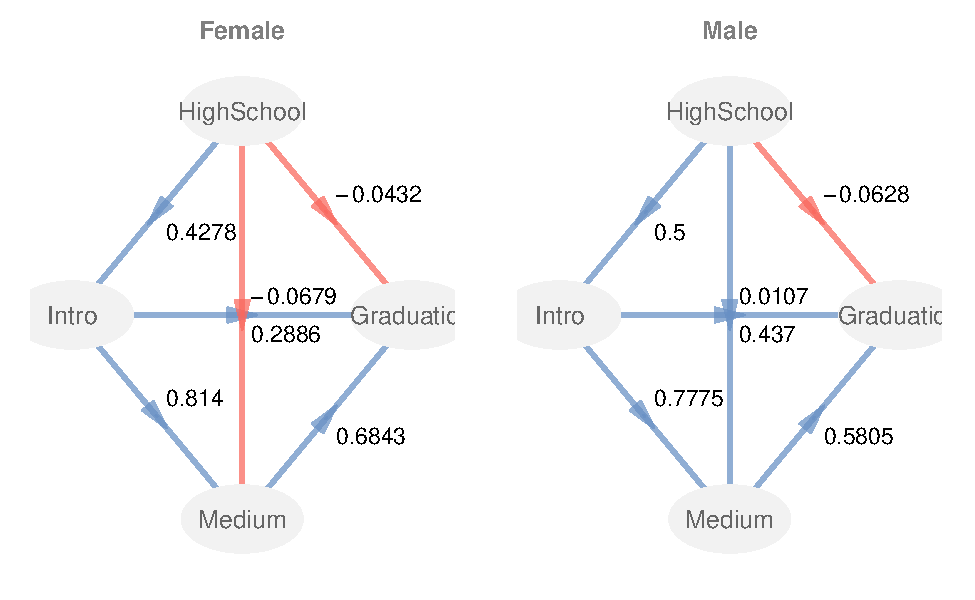
\includegraphics[width=1\linewidth,height=.55\linewidth]{figure/gpa_fem_male_models} 

}

\caption[Path Coefficients of Female and Male Students]{Path Coefficients of Female and Male Students\label{fig:gpa_fem_male_models}}
\end{figure}


\end{knitrout}


Numerically, we have different path coefficients between both models. This is what we would expect to happen in real life because of differences in the data. But the important question is \textit{how different the path coefficients really are?}. Let's take the effect of \texttt{HighSchool} on \texttt{Intro} for example. It has a value of 0.4278 in Female students and 0.5 in Male students. For some people this might be a considerable difference while for others it might be something negligible. We definitely need to perform some group analysis to get a verdict.



\section{Comparing Groups: Bootstrap t-test}
\plspm{} comes with the function \code{plspm.groups()} that allows us to apply the bootstrap approach and the permutation approach to compare groups in PLS Path Modeling. The standard usage of \code{plspm.groups()} is:

\texttt{plspm.groups(pls, group, method, reps)}

The first argument \code{pls} is an object of class \code{"plspm"}; \code{group} must be a categorical variable (codified as an R \code{factor}) with two levels indicating the groups to be compared; \code{method} indicates the applied approach; and \code{reps} is the number of resamples (100 by default). 

In order to apply the bootstrap procedure we use the parameter \code{method="bootstrap"}:
\begin{knitrout}
\definecolor{shadecolor}{rgb}{0.969, 0.969, 0.969}\color{fgcolor}\begin{kframe}
\begin{alltt}
\hlcomment{# apply plspm.groups bootstrap}
gpa_boot = \hlfunctioncall{plspm.groups}(gpa_pls, college$Gender, method = \hlstring{"bootstrap"})

\hlcomment{# see the results}
gpa_boot
\end{alltt}
\begin{verbatim}
## GROUP COMPARISON IN PLS-PM FOR PATH COEFFICIENTS 
## 
## Scale of Data:       TRUE 
## Weighting Scheme:    centroid 
## Selected method:     bootstrap 
## Num of replicates:   100 
## 
## $test 
##                          global  group.FEMALE  group.MALE  diff.abs
## HighSchool->Intro        0.4531        0.4278      0.5000    0.0722
## HighSchool->Medium      -0.0460       -0.0679      0.0107    0.0786
## HighSchool->Graduation  -0.0488       -0.0432     -0.0628    0.0197
## Intro->Medium            0.7996        0.8140      0.7775    0.0365
## Intro->Graduation        0.3438        0.2886      0.4370    0.1484
## Medium->Graduation       0.6439        0.6843      0.5805    0.1038
##                         t.stat  deg.fr  p.value  sig.05
## HighSchool->Intro       0.8061     350   0.2104      no
## HighSchool->Medium      1.1477     350   0.1259      no
## HighSchool->Graduation  0.7484     350   0.2274      no
## Intro->Medium           0.8168     350   0.2073      no
## Intro->Graduation       1.5996     350   0.0553      no
## Medium->Graduation      1.1636     350   0.1227      no
## 
## Inner models in the following objects: 
## $global  
## $group1  
## $group2
\end{verbatim}
\end{kframe}
\end{knitrout}

The first part of the output is a description with the specified parameters: \code{scaled} and \code{scheme} belong to the arguments specified in \code{pls}; the \code{method} and the \code{replicates} belong to the selected approaches and the number of resamples. 

The second part is the data frame contained in \code{\$test}. The first column \code{global} shows the path coefficients of the global model; the second and third columns show the path coefficients of the compared groups (\code{FEMALE} and \code{MALE}, respectively). The fourth column \code{diff.abs} is the absolute difference of path coefficients between female and male studetns. Then we have the columns \code{t.stat}, \code{deg.fr}, and \code{p.value} that contain the statistic of the $t$-test with its degrees of freedom and the associated p-value. The last column \code{sig.05} is just an auxiliary label to indicate whether the difference in path coefficients is significant at the 5\% level. As we can see from the obtained results, none of the path coefficients between females and males are significantly different.



\section{Comparing Groups: Permutation test}
In order to apply the permutation procedure we have to specify the parameter \code{method = } \code{"permutation"} inside the function \code{plspm.groups()}:
\begin{knitrout}
\definecolor{shadecolor}{rgb}{0.969, 0.969, 0.969}\color{fgcolor}\begin{kframe}
\begin{alltt}
\hlcomment{# apply plspm.groups premutation}
gpa_perm = \hlfunctioncall{plspm.groups}(gpa_pls, college$Gender, method = \hlstring{"permutation"})

\hlcomment{# see the results}
gpa_perm
\end{alltt}
\begin{verbatim}
## GROUP COMPARISON IN PLS-PM FOR PATH COEFFICIENTS 
## 
## Scale of Data:       TRUE 
## Weighting Scheme:    centroid 
## Selected method:     permutation 
## Num of replicates:   100 
## 
## $test 
##                          global  group.FEMALE  group.MALE  diff.abs
## HighSchool->Intro        0.4531        0.4278      0.5000    0.0722
## HighSchool->Medium      -0.0460       -0.0679      0.0107    0.0786
## HighSchool->Graduation  -0.0488       -0.0432     -0.0628    0.0197
## Intro->Medium            0.7996        0.8140      0.7775    0.0365
## Intro->Graduation        0.3438        0.2886      0.4370    0.1484
## Medium->Graduation       0.6439        0.6843      0.5805    0.1038
##                         p.value  sig.05
## HighSchool->Intro        0.4059      no
## HighSchool->Medium       0.3069      no
## HighSchool->Graduation   0.5545      no
## Intro->Medium            0.5050      no
## Intro->Graduation        0.1386      no
## Medium->Graduation       0.2277      no
## 
## Inner models in the following objects: 
## $global  
## $group1  
## $group2
\end{verbatim}
\end{kframe}
\end{knitrout}

The output in this case is very similar to the bootstrap procedure except that that data frame \code{\$test} only contains the p-value. As we the bootstrap $t$-test, none of the path coefficients' differences are significant (at the 5\% level).


\subsection*{Show me the numbers}
Finally, we can get an additional visualization of the differences in path coefficients between females by creating a barplot like this one:
\begin{knitrout}
\definecolor{shadecolor}{rgb}{0.969, 0.969, 0.969}\color{fgcolor}\begin{figure}[h]


{\centering 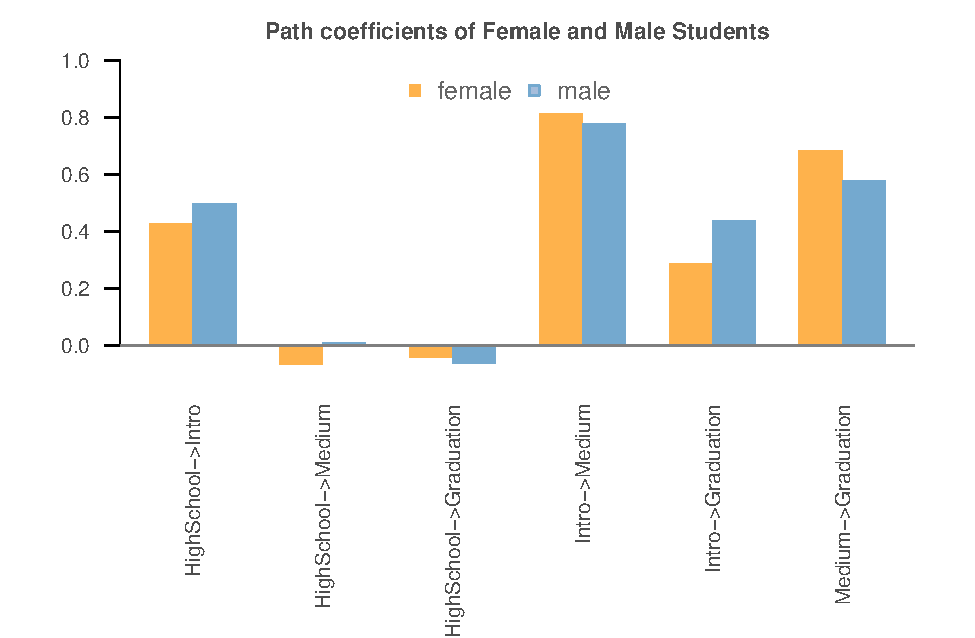
\includegraphics[width=.85\linewidth,height=.625\linewidth]{figure/female_male_barplot} 

}

\caption[Barplot of path coefficients between female and male students]{Barplot of path coefficients between female and male students\label{fig:female_male_barplot}}
\end{figure}


\end{knitrout}



\begin{knitrout}
\definecolor{shadecolor}{rgb}{0.969, 0.969, 0.969}\color{fgcolor}\begin{kframe}
\begin{alltt}
\hlcomment{# path coefficients between female and male students}
\hlfunctioncall{barplot}(\hlfunctioncall{t}(\hlfunctioncall{as.matrix}(gpa_boot$test[,2:3])), border = NA, beside = TRUE, 
        col = \hlfunctioncall{c}(\hlstring{"#FEB24C"},\hlstring{"#74A9CF"}), las = 2, ylim = \hlfunctioncall{c}(-0.1, 1), 
        cex.names = 0.8, col.axis = \hlstring{"gray30"}, cex.axis = 0.8)
\hlcomment{# add horizontal line}
\hlfunctioncall{abline}(h = 0, col = \hlstring{"gray50"})
\hlcomment{# add itle}
\hlfunctioncall{title}(\hlstring{"Path coefficients of Female and Male Students"}, 
      cex.main = 0.95, col.main = \hlstring{"gray30"})
\hlcomment{# add legend}
\hlfunctioncall{legend}(\hlstring{"top"}, legend = \hlfunctioncall{c}(\hlstring{"female"}, \hlstring{"male"}), pt.bg = \hlfunctioncall{c}(\hlstring{"#FEB24C"}, \hlstring{"#A6BDDB"}), 
       ncol = 2, pch = 22, col = \hlfunctioncall{c}(\hlstring{"#FEB24C"}, \hlstring{"#74A9CF"}), bty = \hlstring{"n"}, 
       text.col = \hlstring{"gray40"})
\end{alltt}
\end{kframe}
\end{knitrout}




\section{Reading List}
\begin{itemize}
 \vspace{2mm}
 \item \textbf{\textsf{Multi-Group analysis with PLS}} by Wynne Chin (2000) In his outdated but still active website, Wynne Chin describes the bootstrap t-test for multi-group comparisons. Available online in the section \textit{Frequently Asked Questions - Partial Least Squares \& PLS-Graph} at: \\ 
 \texttt{\href{http://disc-nt.cba.uh.edu/chin/plsfaq/multigroup.htm}{http://disc-nt.cba.uh.edu/chin/plsfaq/multigroup.htm}}

 \vspace{2mm}
 \item \textbf{\textsf{An Introduction to a Permutation Based Procedure for Multi-Group PLS Analysis}} by Wynne Chin and Jens Dibbern (2010). Published as Chapter 7 of the \textit{Handbook of Partial Least Squares}, this article provides a basic introduction to the permutation approach for multi-group comparison. Wynne and Jens also provide a simple example application of cross-cultural analysis with an Information System model. 
 
 \vspace{2mm}
 \item \textbf{\textsf{Use of ULS-SEM and PLS-SEM to Measure a Group Effect in a Regression Model Relating Two Blocks of Binary Variables}} by Michel Tenenhaus, Emmanuelle Mauger and Christiane Guinot (2010). Published as Chapter 5 of the \textit{Handbook of Partial Least Squares}, this article proposes an interesting alternative way for comparing groups. Although the discussed example in this article uses a covariance-based structural modeling approach (ULS-SEM with AMOS 6.0), the methodology can be adapted to PLS-PM. 
 
\end{itemize}


% Chapter7

% !Rnw root = ../PLS_Path_Modeling_with_R.Rnw


\chapter{Moderating Effects}
One of the analysis tasks that arises from time to time when studying path models is the examination of the so-called \textit{moderating effects}, also known as \textit{interaction effects}. In short, this type of effect represents the influence that a third variable has on the relationship between an independent and a dependent variable. This chapter is dedicated to show you how to test moderating effects with \plspm{}. 


\section{Moderator Variables}
If you are dealing with testing moderating effects, chances are that you will encounter some type of definition like the one below:

\begin{quotation} \noindent
A moderating effect is caused by  a variable ($M$) whose variation influences the strength or the direction of a relationship between an independent variable ($X$) and a dependent variable ($Y$). 
\end{quotation}

If you are like me, don't worry if you haven't grasped the notion of a moderating effect from the previous definition (you're not alone). A moderating effect is the fancy term that some authors use to say that there is a nosy variable $M$ influencing the effect between an independent variable $X$ and a dependent variable $Y$. Not surprinsingly, the nosy variable $M$ is called a \textit{moderator} variable and it can be a qualitative or a quantitative variable. Common examples of qualitative moderator variables are things like Gender or Ethnicity; in turn, quantitative moderator variables are things like Age or Income.

Perhaps a better way to explain the concept of a moderating effect is by using a graphical display. The following figure is a typical diagram showing the effect of a moderator variable. We have three variables: an independent variable $X$, a dependent variable $Y$, and the moderator variable $M$. It is assumed that there is a causal relationship between $X$ and $Y$. The key component in the diagram is the dashed arrow from $M$ affecting the arrow between $X$ and $Y$. This dashed line represents the moderating effect of $M$, which is supposed to influence the \textbf{strength} and/or \textbf{direction} that $X$ has on $Y$.




\begin{knitrout}
\definecolor{shadecolor}{rgb}{0.969, 0.969, 0.969}\color{fgcolor}\begin{figure}[h]


{\centering 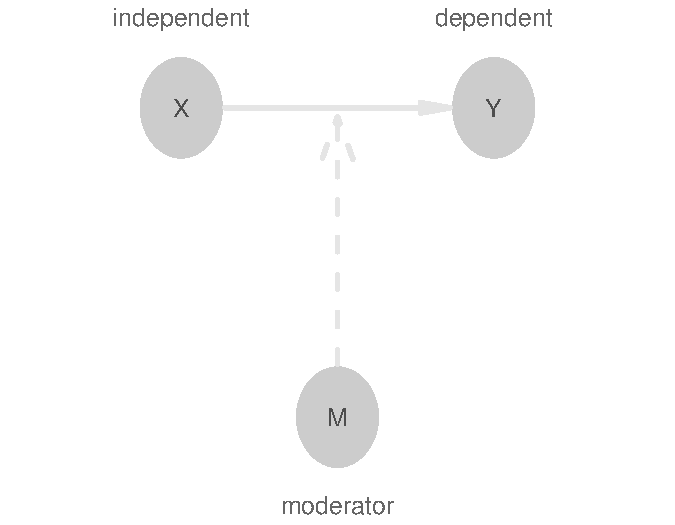
\includegraphics[width=.7\linewidth,height=.4\linewidth]{figure/typical_moderator} 

}

\caption[Typical diagram illustrating the effect of a nosy moderator variable]{Typical diagram illustrating the effect of a nosy moderator variable\label{fig:typical_moderator}}
\end{figure}


\end{knitrout}


This diagram is just for illustration purposes. Keep in mind that this diagram is an abstract representation; it's not a path diagram that you are supposed to figure out how to implement in PLS-PM software.



\section{Moderating effects in PLS-PM}
The general concepts of moderating effects and moderator variables have their own adaptation and representation in the PLS-PM world. Basically, there are two main options to study moderating effects depending on the nature of the moderator variable:

\begin{itemize}
 \item \textbf{Group Comparisons} This approach has to do when the moderator is qualitative (i.e. categorical) like Age or Gender, or when the moderator can be categorized. In this case we should use one of the methods discussed in Chapter 6 for comparing groups ---\plspm{} comes with the function \code{plspm.groups()} that is designed to compare two models by providing a categorical variable (an R \code{factor}) with two categories---.
 
 \item \textbf{Moderator Constructs} This approach has to do when the moderator variable is treated as a latent variable. Under this approach, moderator variables are only considered in the inner model (the structural part of a path model).
\end{itemize}


\subsection{Moderator variables as constructs}
When moderator variables are to be included in the model, the most important thing you need to know is that they have to be considered in the inner model. This means that moderating effects are treated as latent variables. In PLS-PM, we can find four main ways to study the effects of latent moderator variables: 
\begin{itemize}
 \item by using a \textbf{Product Indicator Approach}
 \item by using a \textbf{Two-Stage Path Modeling Approach}
 \item by using a \textbf{Two-Stage Regression Approach}
 \item by using a \textbf{Categorical Variable Approach}
\end{itemize}
In the following sections we'll describe each of these approaches.



\subsection{Case Study: Simplified Customer Satisfaction}
In this example we are going to consider a simplified version of the Customer Satisfaction Index model with three latent variables: Image, Satisfaction and Loyalty. 



\begin{knitrout}
\definecolor{shadecolor}{rgb}{0.969, 0.969, 0.969}\color{fgcolor}\begin{figure}[h]


{\centering 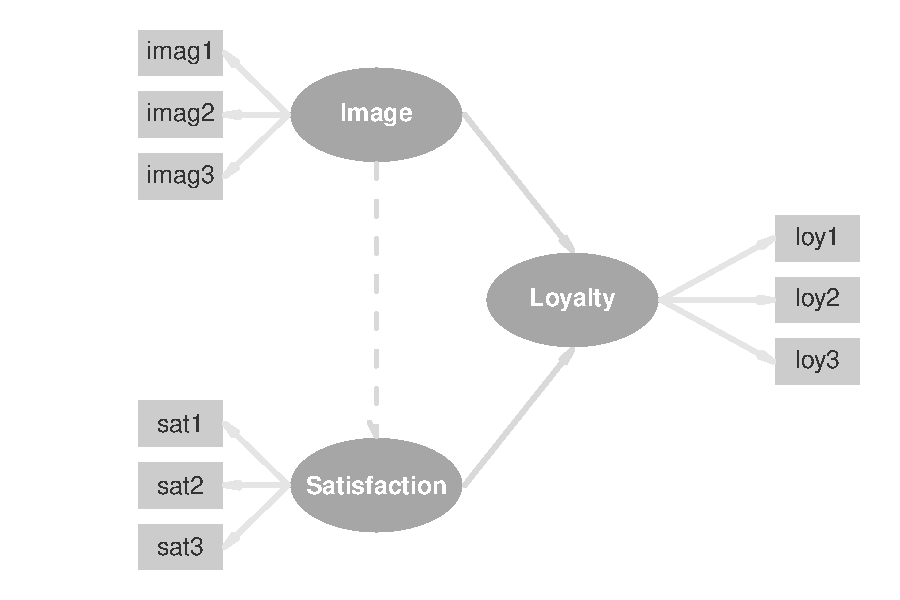
\includegraphics[width=.8\linewidth,height=.5\linewidth]{figure/simple_ecsi_diag} 

}

\caption[Simplified Customer Satisfaction Model]{Simplified Customer Satisfaction Model\label{fig:simple_ecsi_diag}}
\end{figure}


\end{knitrout}


The model is focused on Loyalty and we are assuming that it depends on the Perceived Image and the Customer Satisfaction. The better the Perceived Image as well as the Satisfaction, the more Loyals will be the customers. To keep things simple, each block will have three indicators. For whatever reason you like to think of, let's assume that Image plays the role of a moderator variable. That's why there is a dashed arrow from Image to Satisfaction. In summary, there is going to be a main effect of Image on Loyalty, but there is also going to be a moderating effect of Image in the relationship between Satisfaction and Loyalty.



\section{Product Indicator Approach}
The first approach we will describe for analyzing moderating effects in PLS Path Modeling is the \textbf{Product Indicator Approach}. In this approach we seek to create a new latent variable that represents the interaction between the exogenous variable and the moderator variable. How do we create this new latent variable? As its name says, the idea behind the Product Inicator Approach is to build \textbf{product} terms between the \textbf{indicators} of the independent latent variable and the indicators of the moderator latent variable. These product terms are the indicators that we use for the latent interaction term in the structural model. Last but not least, we always treat the created interaction construct as a \textbf{reflective construct}.





\begin{knitrout}
\definecolor{shadecolor}{rgb}{0.969, 0.969, 0.969}\color{fgcolor}\begin{figure}[h]


{\centering 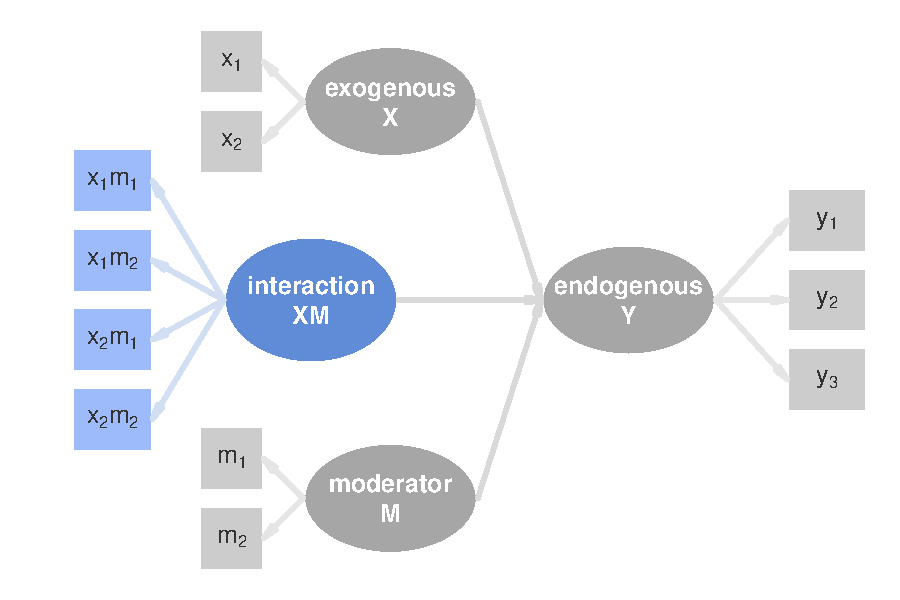
\includegraphics[width=.8\linewidth,height=.5\linewidth]{figure/prod_ind_app_diag} 

}

\caption[Diagram of a Product Indicator latent variable (XM)]{Diagram of a Product Indicator latent variable (XM)\label{fig:prod_ind_app_diag}}
\end{figure}


\end{knitrout}


A better way to understand the Product Indicator Approach is by looking at a simple example shown in figure 2.3. Let's say we have three reflective constructs: an exogenous $X$, a moderator $M$ (also exogenous), and an endogenous $Y$. Let's suppose that $X$ and $M$ have two indicators, and that $Y$ has three indicators. To estimate the moderating effect, we need to create a new latent interaction term $XM$ whose indicators will be the products of the indicators of $X$ and $M$.


\subsection{Example}
Let's see how to test for moderating effects with the Product Indicator Approach in \plspm{}. As we mentioned above, we will treat Image as the moderator variable in our simplified customer satisfaction model: Image moderates the effect that Satisfaction has on Loyalty. This implies that we will have three indicators (\code{Image}, \code{Satisfaction}, and \code{Loyalty}) plus a new latent construct, \texttt{Inter}, representing the product interaction of \code{Image} and \code{Satisfaction}. The new latent construct \texttt{Inter} will be measured by the product terms of the indicators of both \texttt{Image} and \texttt{Satisfaction}. See the following diagram:




\begin{knitrout}
\definecolor{shadecolor}{rgb}{0.969, 0.969, 0.969}\color{fgcolor}\begin{figure}[h]


{\centering 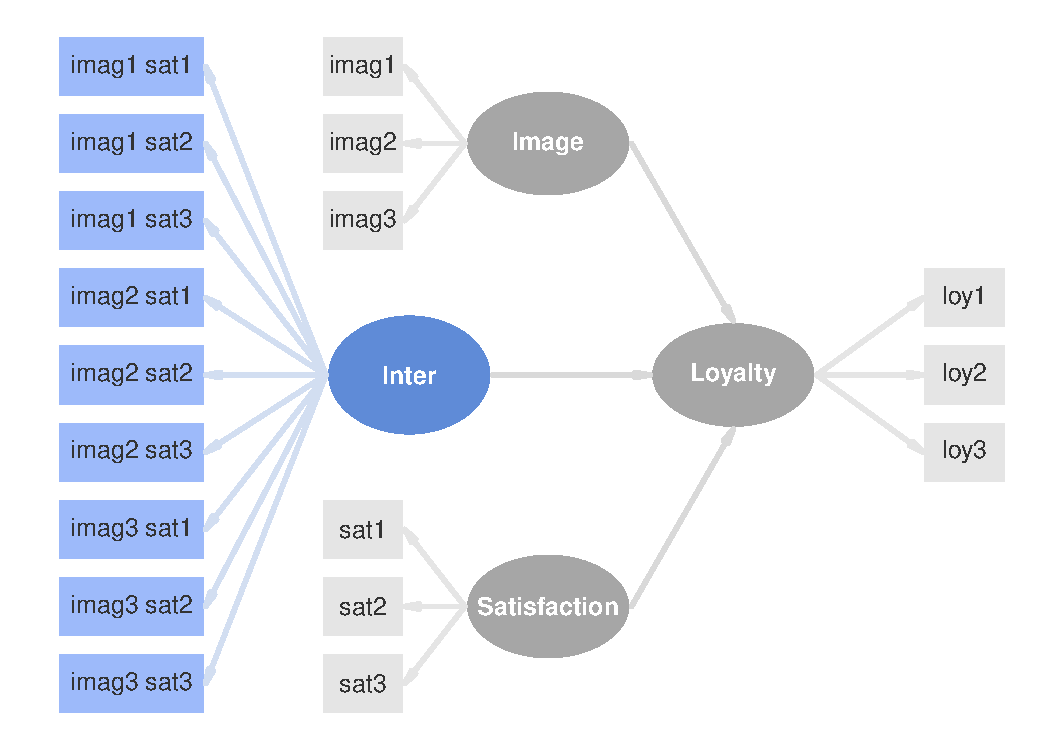
\includegraphics[width=.8\linewidth,height=.6\linewidth]{figure/prod_ind_app_sat_diag} 

}

\caption[Customer Satisfaction Model with a Product Indicator latent variable (Inter)]{Customer Satisfaction Model with a Product Indicator latent variable (Inter)\label{fig:prod_ind_app_sat_diag}}
\end{figure}


\end{knitrout}




\subsubsection*{Step 1}
First thigs first, let's load the \plspm{} package and let's get the data \code{satisfaction}: 
\begin{knitrout}
\definecolor{shadecolor}{rgb}{0.969, 0.969, 0.969}\color{fgcolor}\begin{kframe}
\begin{alltt}
\hlcomment{# load package 'plspm'}
\hlfunctioncall{library}(\hlstring{"plspm"})

\hlcomment{# get data satisfaction}
\hlfunctioncall{data}(satisfaction)
\end{alltt}
\end{kframe}
\end{knitrout}


Our initial step is to create the product-indicators of the new moderating latent variable \texttt{Inter}. 
This means we need to calculate the products between the three indicators of \texttt{Image} and the three indicators of \texttt{Satisfaction}. For convenience, we will ``duplicate'' the data frame \code{satisfaction} in another data frame: \code{satisfaction1};
\begin{knitrout}
\definecolor{shadecolor}{rgb}{0.969, 0.969, 0.969}\color{fgcolor}\begin{kframe}
\begin{alltt}
\hlcomment{# duplicate satisfaction as satisfaction1}
satisfaction1 = satisfaction

\hlcomment{# how many columns in satisfaction1?}
\hlfunctioncall{ncol}(satisfaction1)
\end{alltt}
\begin{verbatim}
## [1] 28
\end{verbatim}
\end{kframe}
\end{knitrout}


Once we have the new (duplicated) data frame we will add the product terms as new columns in \code{satisfaction1}. To check we have more added columns simply inspect the number of columns with \code{ncol()}
\begin{knitrout}
\definecolor{shadecolor}{rgb}{0.969, 0.969, 0.969}\color{fgcolor}\begin{kframe}
\begin{alltt}
\hlcomment{# create product indicator terms between Image and Satisfaction}
satisfaction1$inter1 = satisfaction$imag1 * satisfaction$sat1
satisfaction1$inter2 = satisfaction$imag1 * satisfaction$sat2
satisfaction1$inter3 = satisfaction$imag1 * satisfaction$sat3
satisfaction1$inter4 = satisfaction$imag2 * satisfaction$sat1
satisfaction1$inter5 = satisfaction$imag2 * satisfaction$sat2
satisfaction1$inter6 = satisfaction$imag2 * satisfaction$sat3
satisfaction1$inter7 = satisfaction$imag3 * satisfaction$sat1
satisfaction1$inter8 = satisfaction$imag3 * satisfaction$sat2
satisfaction1$inter9 = satisfaction$imag3 * satisfaction$sat3

\hlcomment{# check again the number of columns in satisfaction1}
\hlfunctioncall{ncol}(satisfaction1)
\end{alltt}
\begin{verbatim}
## [1] 37
\end{verbatim}
\end{kframe}
\end{knitrout}

Originally, the data \code{satisfaction1} contained 28 variables, but we added nine more variables with the creation of the product-indicator terms. Now we should have a total of 37 columns in the duplicated data set.

\subsubsection{Step 2}
We proceed as usual with the definition of the ingredients for our PLS-PM cook recipe: a path matrix for the inner model, a list of \code{blocks} for the outer model list, and a vector for the measurement modes. Additionally, we'll run the \fplspm{} function with bootstrap validation (200 resamples).
\begin{knitrout}
\definecolor{shadecolor}{rgb}{0.969, 0.969, 0.969}\color{fgcolor}\begin{kframe}
\begin{alltt}
\hlcomment{# create path matrix}
r1 = \hlfunctioncall{c}(0, 0, 0, 0)
r2 = \hlfunctioncall{c}(0, 0, 0, 0)
r3 = \hlfunctioncall{c}(0, 0, 0, 0)
r4 = \hlfunctioncall{c}(1, 1, 1, 0)
prod_path = \hlfunctioncall{rbind}(r1, r2, r3, r4)
\hlfunctioncall{rownames}(prod_path) = \hlfunctioncall{c}(\hlstring{"Image"}, \hlstring{"Inter"}, \hlstring{"Satisfaction"}, \hlstring{"Loyalty"})
\hlfunctioncall{colnames}(prod_path) = \hlfunctioncall{c}(\hlstring{"Image"}, \hlstring{"Inter"}, \hlstring{"Satisfaction"}, \hlstring{"Loyalty"})

\hlcomment{# define outer model list}
prod_blocks = \hlfunctioncall{list}(1:3, 29:37, 20:22, 24:26)

\hlcomment{# define reflective indicators}
prod_modes = \hlfunctioncall{rep}(\hlstring{"A"}, 4)

\hlcomment{# run plspm analysis with bootstrap validation}
prod_pls = \hlfunctioncall{plspm}(satisfaction1, prod_path, prod_blocks, modes = prod_modes, 
                 boot.val = TRUE, br = 200)
\end{alltt}
\end{kframe}
\end{knitrout}



\subsubsection*{Step 3}
After running the PLS-PM analysis, we check the obtained path coefficients:
\begin{knitrout}
\definecolor{shadecolor}{rgb}{0.969, 0.969, 0.969}\color{fgcolor}\begin{kframe}
\begin{alltt}
\hlcomment{# check path coefficients}
prod_pls$path_coefs
\end{alltt}
\begin{verbatim}
##               Image    Inter Satisfaction Loyalty
## Image        0.0000  0.00000       0.0000       0
## Inter        0.0000  0.00000       0.0000       0
## Satisfaction 0.0000  0.00000       0.0000       0
## Loyalty      0.2999 -0.04576       0.5226       0
\end{verbatim}
\end{kframe}
\end{knitrout}


Looking at the path coefficients you can see that the moderating product construct \texttt{Inter} has a negative effect on \texttt{Loyalty}
\begin{knitrout}
\definecolor{shadecolor}{rgb}{0.969, 0.969, 0.969}\color{fgcolor}\begin{kframe}
\begin{alltt}
\hlcomment{# plot inner model}
\hlfunctioncall{plot}(prod_pls)
\end{alltt}
\end{kframe}
\end{knitrout}


\begin{knitrout}
\definecolor{shadecolor}{rgb}{0.969, 0.969, 0.969}\color{fgcolor}\begin{figure}[h]


{\centering 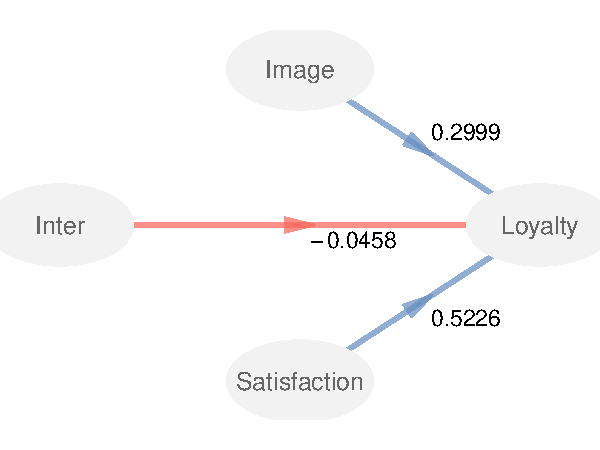
\includegraphics[width=.6\linewidth,height=.4\linewidth]{figure/ProdIndApp_plot_inner} 

}

\caption[Inner model with path coefficients]{Inner model with path coefficients\label{fig:ProdIndApp_plot_inner}}
\end{figure}


\end{knitrout}



In order to confirm the significance of the path coefficients, we need to check the bootstrap results contained in \code{\$boot\$paths}:
\begin{knitrout}
\definecolor{shadecolor}{rgb}{0.969, 0.969, 0.969}\color{fgcolor}\begin{kframe}
\begin{alltt}
\hlcomment{# check bootstrapped path coefficients}
prod_pls$boot$paths
\end{alltt}
\begin{verbatim}
##                         Original Mean.Boot Std.Error perc.025
## Image -> Loyalty         0.29995   0.31426    0.1306  0.07353
## Inter -> Loyalty        -0.04576  -0.06969    0.2187 -0.55044
## Satisfaction -> Loyalty  0.52257   0.54001    0.1471  0.25293
##                         perc.975
## Image -> Loyalty          0.5572
## Inter -> Loyalty          0.2928
## Satisfaction -> Loyalty   0.8581
\end{verbatim}
\end{kframe}
\end{knitrout}

Even though \texttt{Inter} has a negative effect on \texttt{Loyalty}, its associated bootstrap confidence interval contains the zero, having a non-significant effect. This means that the moderating effect of \texttt{Inter} on the relation between \texttt{Satisfaction} and \texttt{Loyalty} is not significant.




\section{Two-Stage Path Modeling Approach}
Another approach for testing moderating effects is to use a \textbf{two-stage path modeling approach}. As the name indicates, this approach involves two stages: the first stage consists of applying a PLS-PM analysis without the interaction term; the second stage consists of taking the scores obtained in the first stage for creating the interaction term, and then perform a second PLS-PM analysis including the scores as indicators of the constructs:



\begin{knitrout}
\definecolor{shadecolor}{rgb}{0.969, 0.969, 0.969}\color{fgcolor}

{\centering 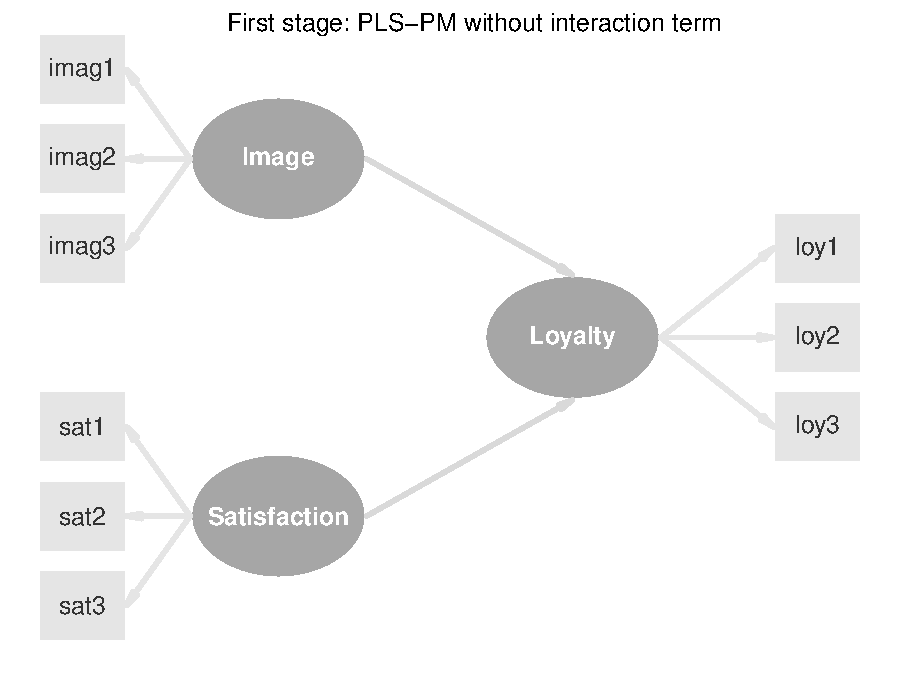
\includegraphics[width=.7\linewidth,height=.45\linewidth]{figure/TwoStageApp1_diag} 

}



\end{knitrout}






\begin{knitrout}
\definecolor{shadecolor}{rgb}{0.969, 0.969, 0.969}\color{fgcolor}

{\centering 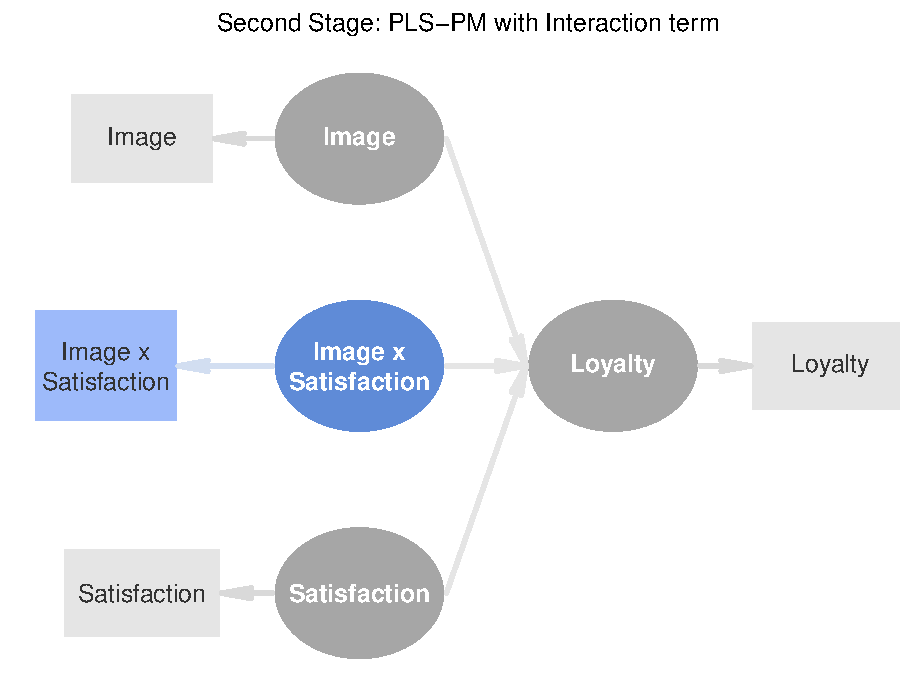
\includegraphics[width=.7\linewidth,height=.4\linewidth]{figure/TwoStageApp2_diag} 

}



\end{knitrout}


\subsection{Example}
To apply the Two-Stage Path Modeling Approach with \plspm{} we begin with a first PLS-PM analysis that includes just the main effects (no interaction terms).


\subsubsection*{Stage 1}
We apply a first PLS-PM analysis with \code{Image}, \code{Satisfaction} and \code{Loyalty}:
\begin{knitrout}
\definecolor{shadecolor}{rgb}{0.969, 0.969, 0.969}\color{fgcolor}\begin{kframe}
\begin{alltt}
\hlcomment{# create path matrix}
f1 = \hlfunctioncall{c}(0, 0, 0)
f2 = \hlfunctioncall{c}(0, 0, 0)
f3 = \hlfunctioncall{c}(1, 1, 0)
first_path = \hlfunctioncall{rbind}(f1, f2, f3)
\hlfunctioncall{rownames}(first_path) = \hlfunctioncall{c}(\hlstring{"Image"}, \hlstring{"Satisfaction"}, \hlstring{"Loyalty"})

\hlcomment{# define list of blocks}
first_blocks = \hlfunctioncall{list}(1:3, 20:22, 24:26)

\hlcomment{# define reflective indicators}
first_modes = \hlfunctioncall{rep}(\hlstring{"A"}, 3)

\hlcomment{# run plspm analysis}
first_pls = \hlfunctioncall{plspm}(satisfaction, first_path, first_blocks, modes = first_modes)
\end{alltt}
\end{kframe}
\end{knitrout}


\subsubsection*{Stage 2: Step 1}
The second stage involves applying another PLS-PM analysis but this time using the scores obtained in the first stage. This implies that we use the latent variable scores from stage 1 in order to create the interaction term \texttt{Inter = Image x Satisfaction}. For convenience, we can put the scores in \texttt{data.frame} format so we can plot their corresponding densities:
\begin{knitrout}
\definecolor{shadecolor}{rgb}{0.969, 0.969, 0.969}\color{fgcolor}\begin{kframe}
\begin{alltt}
\hlcomment{# get the latent variable scores in data frame format}
Scores = \hlfunctioncall{as.data.frame}(first_pls$scores)

\hlcomment{# create the interaction term}
Scores$Inter = Scores$Image * Scores$Satisfaction

\hlcomment{# let's see how Scores look like}
\hlfunctioncall{head}(Scores, n = 5)
\end{alltt}
\begin{verbatim}
##    Image Satisfaction Loyalty     Inter
## 1 0.3363     -0.34526  0.4094 -0.116098
## 2 0.9700      0.39697  0.5686  0.385073
## 3 0.2747      0.79596  0.7571  0.218678
## 4 0.3184      0.02585 -0.6877  0.008232
## 5 0.8907      0.58825  0.7322  0.523935
\end{verbatim}
\end{kframe}
\end{knitrout}


To depict the densities of the scores, we can use the function \code{density()} and plot it with the help of \code{plot()} and \code{polygon()}
\begin{knitrout}
\definecolor{shadecolor}{rgb}{0.969, 0.969, 0.969}\color{fgcolor}\begin{kframe}
\begin{alltt}
\hlcomment{# setting graphical parameters}
op = \hlfunctioncall{par}(mfrow = \hlfunctioncall{c}(2, 2), mar = \hlfunctioncall{c}(4, 5, 2, 2), bty = \hlstring{"n"})
\hlcomment{# for each scores}
\hlfunctioncall{for} (j in 1:4)
\{
\hlcomment{   # calculate density }
   score.dens = \hlfunctioncall{density}(Scores[,j])
\hlcomment{   # plot window but don't show the density}
   \hlfunctioncall{plot}(score.dens, main = \hlfunctioncall{names}(Scores)[j], xlab = \hlstring{""}, type = \hlstring{"n"})
\hlcomment{   # add polygon}
   \hlfunctioncall{polygon}(score.dens$x, score.dens$y, col = \hlstring{"gray90"}, border = \hlstring{"gray80"})
\}
\hlcomment{# reset deafult values of graphical parameters}
\hlfunctioncall{par}(op)
\end{alltt}
\end{kframe}
\end{knitrout}


\begin{knitrout}
\definecolor{shadecolor}{rgb}{0.969, 0.969, 0.969}\color{fgcolor}

{\centering 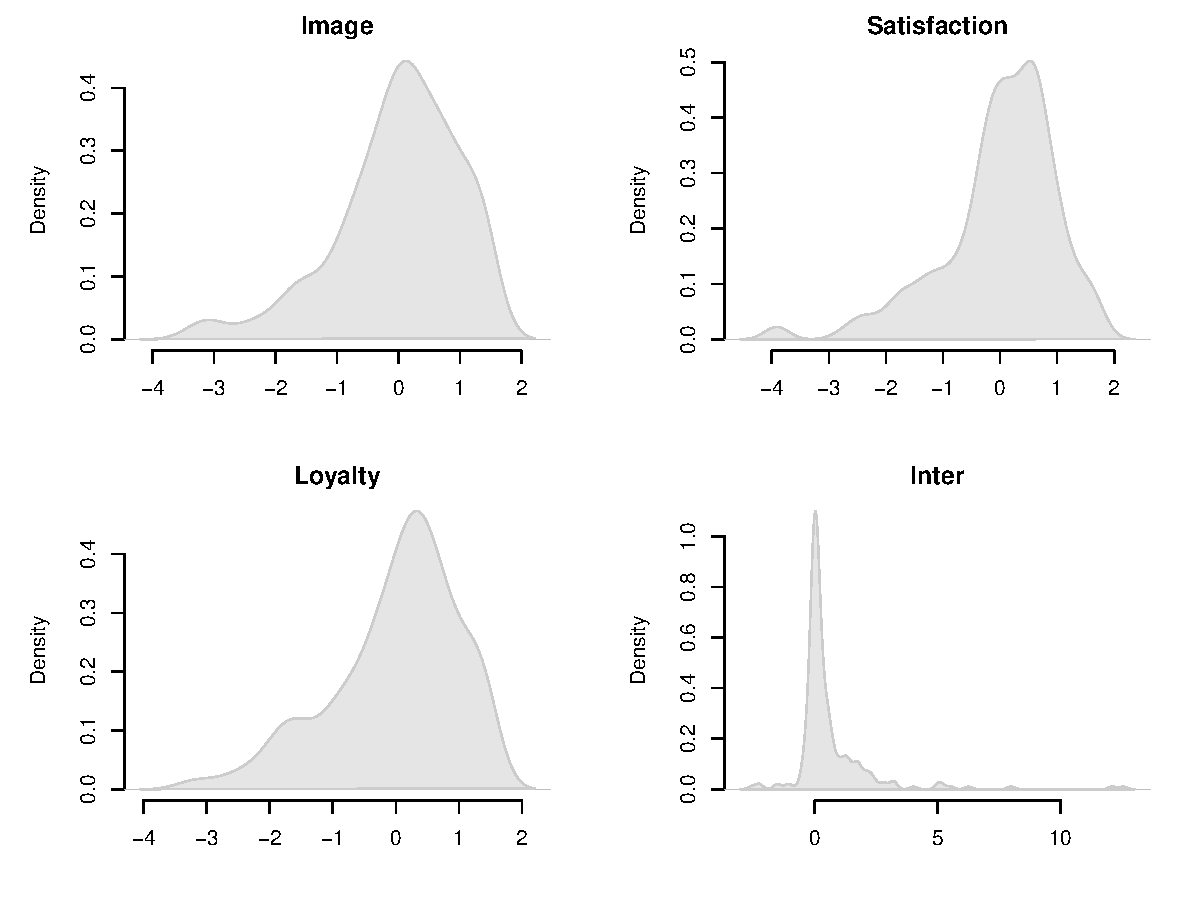
\includegraphics[width=.95\linewidth,height=.6\linewidth]{figure/TwoStageApp1_distr_plot} 

}



\end{knitrout}



\subsubsection*{Stage 2: Step 2}
Once we created the interaction term \code{Inter}, the second stage consists of running another PLS-PM analysis but now we replace the original indicators by the scores obtained in the previous stage:
\begin{knitrout}
\definecolor{shadecolor}{rgb}{0.969, 0.969, 0.969}\color{fgcolor}\begin{kframe}
\begin{alltt}
\hlcomment{# create path matrix}
two_path = \hlfunctioncall{matrix}(\hlfunctioncall{c}(0,0,0,0,0,0,0,0,0,0,0,0,1,1,1,0), 
                  nrow = 4, ncol = 4, byrow = TRUE)
\hlfunctioncall{rownames}(two_path) = \hlfunctioncall{c}(\hlstring{"Image"}, \hlstring{"Inter"}, \hlstring{"Satisfaction"}, \hlstring{"Loyalty"})
\hlfunctioncall{colnames}(two_path) = \hlfunctioncall{c}(\hlstring{"Image"}, \hlstring{"Inter"}, \hlstring{"Satisfaction"}, \hlstring{"Loyalty"})

\hlcomment{# define list of blocks}
two_blocks = \hlfunctioncall{list}(1, 4, 2, 3)

\hlcomment{# define reflective indicators}
two_modes= \hlfunctioncall{rep}(\hlstring{"A"}, 4)

\hlcomment{# run plspm analysis with bootstrap validation (200 resamples)}
two_pls = \hlfunctioncall{plspm}(Scores, two_path, two_blocks, modes = two_modes, 
                boot.val = TRUE, br = 200)

\hlcomment{# check bootstrap results}
\hlfunctioncall{round}(two_pls$boot$paths, 4)
\end{alltt}
\begin{verbatim}
##                         Original Mean.Boot Std.Error perc.025
## Image -> Loyalty          0.2769    0.2790    0.0669   0.1591
## Inter -> Loyalty         -0.0005   -0.0012    0.0499  -0.0954
## Satisfaction -> Loyalty   0.4957    0.4930    0.0784   0.3428
##                         perc.975
## Image -> Loyalty          0.4204
## Inter -> Loyalty          0.0853
## Satisfaction -> Loyalty   0.6481
\end{verbatim}
\end{kframe}
\end{knitrout}


\begin{knitrout}
\definecolor{shadecolor}{rgb}{0.969, 0.969, 0.969}\color{fgcolor}\begin{kframe}
\begin{alltt}
\hlcomment{# plot inner model}
\hlfunctioncall{plot}(two_pls)
\end{alltt}
\end{kframe}\begin{figure}[h]


{\centering 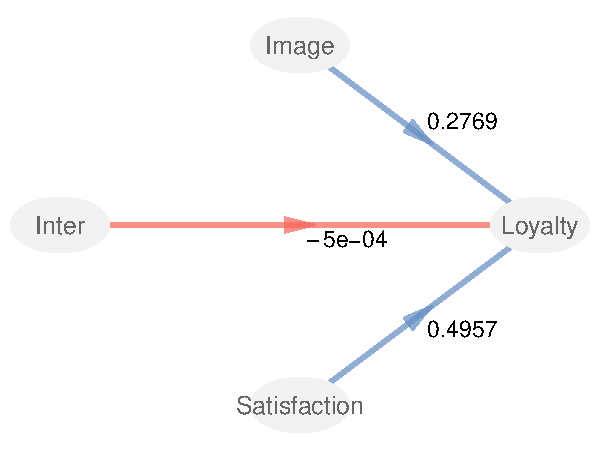
\includegraphics[width=.6\linewidth,height=.4\linewidth]{figure/TwoStageApp_plot_inner} 

}

\caption[Inner model with path coefficients]{Inner model with path coefficients\label{fig:TwoStageApp_plot_inner}}
\end{figure}


\end{knitrout}


As you can see, \texttt{Inter} has a very small effect on \texttt{Loyalty}, and its bootstrap confidence interval contains the zero, having a non-significant effect. This means that the moderating effect of \texttt{Image} on the relation between \texttt{Satisfaction} and \texttt{Loyalty} is not significant.




\section{Two-Stage Regression Approach}
Another alternative for a two-stage procedure is the \textbf{two-stage regression approach}. The first stage is exactly the same as the two-stage path modeling approach: we apply a PLS-PM analysis without the interaction term. The second stage consists of taking the scores obtained in the first stage but, instead of applying another PLS-PM analysis, we apply a regression analysis with the scores of the first stage.

\subsection{Example}
To apply the Two-Stage Regression Approach with \plspm{} we begin in the same way as we did for the two-stage path modeling approach, that is, we start by running a PLS-PM analysis that includes just the main effects (no interaction terms).

\begin{knitrout}
\definecolor{shadecolor}{rgb}{0.969, 0.969, 0.969}\color{fgcolor}\begin{figure}[h]


{\centering 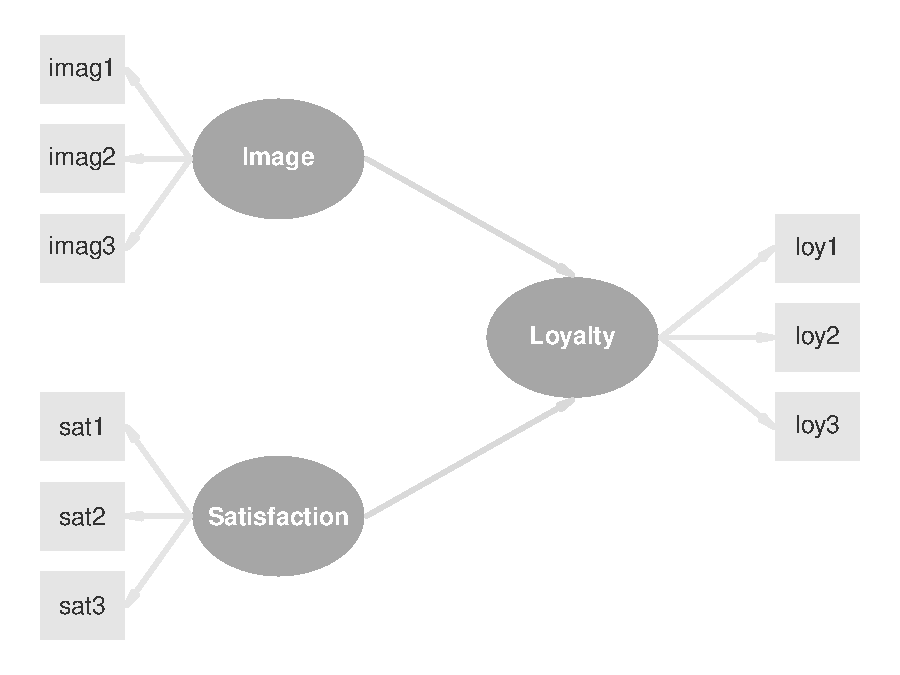
\includegraphics[width=.7\linewidth,height=.45\linewidth]{figure/TwoStageReg1_diag} 

}

\caption[First stage]{First stage: PLS-PM without interaction term\label{fig:TwoStageReg1_diag}}
\end{figure}


\end{knitrout}



\subsubsection*{Stage 1}
For demonstration purposes, we will apply the first stage (which is the same one as in the previous approach):
\begin{knitrout}
\definecolor{shadecolor}{rgb}{0.969, 0.969, 0.969}\color{fgcolor}\begin{kframe}
\begin{alltt}
\hlcomment{# create path matrix}
f1 = \hlfunctioncall{c}(0, 0, 0)
f2 = \hlfunctioncall{c}(0, 0, 0)
f3 = \hlfunctioncall{c}(1, 1, 0)
reg_path = \hlfunctioncall{rbind}(f1, f2, f3)
\hlfunctioncall{rownames}(reg_path) = \hlfunctioncall{c}(\hlstring{"Image"}, \hlstring{"Satisfaction"}, \hlstring{"Loyalty"})

\hlcomment{# define list of blocks}
reg_blocks = \hlfunctioncall{list}(1:3, 20:22, 24:26)

\hlcomment{# define reflective indicators}
reg_modes = \hlfunctioncall{rep}(\hlstring{"A"}, 3)

\hlcomment{# run plspm analysis}
reg_pls = \hlfunctioncall{plspm}(satisfaction, reg_path, reg_blocks, modes = reg_modes)
\end{alltt}
\end{kframe}
\end{knitrout}



\subsubsection*{Stage 2: Step 1}
Once we obtained the scores for \code{Image}, \code{Satisfaction} and \code{Loyalty}, the second stage involves creating the interaction term \texttt{Inter = Image x Satisfaction}, and then applying a regression analysis:
$$Loyalty = b_1 Image + b_2 Satisfaction + b_3 Inter $$

Again, we will put the scores in \texttt{data.frame} format:
\begin{knitrout}
\definecolor{shadecolor}{rgb}{0.969, 0.969, 0.969}\color{fgcolor}\begin{kframe}
\begin{alltt}
\hlcomment{# get the latent variable scores in data frame format}
Scores = \hlfunctioncall{as.data.frame}(reg_pls$scores)

\hlcomment{# create the interaction term}
Scores$Inter = Scores$Image * Scores$Satisfaction

\hlcomment{# let's see how Scores look like}
\hlfunctioncall{head}(Scores, n = 5)
\end{alltt}
\begin{verbatim}
##    Image Satisfaction Loyalty     Inter
## 1 0.3363     -0.34526  0.4094 -0.116098
## 2 0.9700      0.39697  0.5686  0.385073
## 3 0.2747      0.79596  0.7571  0.218678
## 4 0.3184      0.02585 -0.6877  0.008232
## 5 0.8907      0.58825  0.7322  0.523935
\end{verbatim}
\end{kframe}
\end{knitrout}


The path diagram of the second stage is illustrated in the figure below:



\begin{knitrout}
\definecolor{shadecolor}{rgb}{0.969, 0.969, 0.969}\color{fgcolor}\begin{figure}[h]


{\centering 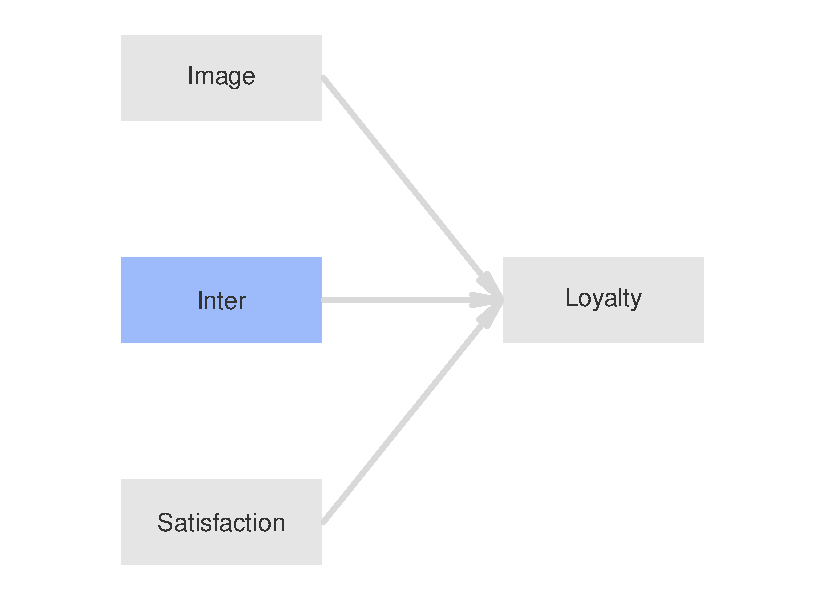
\includegraphics[width=.8\linewidth,height=.45\linewidth]{figure/TwoStageReg2_diag} 

}

\caption[Second Stage]{Second Stage: Regression analysis including the Interaction term\label{fig:TwoStageReg2_diag}}
\end{figure}


\end{knitrout}


\subsubsection*{Stage 2: Step 2}
To perform the regression analysis we will use function \code{lm()} (i.e. linear model) to get the scores:
\begin{knitrout}
\definecolor{shadecolor}{rgb}{0.969, 0.969, 0.969}\color{fgcolor}\begin{kframe}
\begin{alltt}
\hlcomment{# regression analysis}
reg = \hlfunctioncall{lm}(Loyalty ~ Image + Inter + Satisfaction - 1, data = Scores)

\hlcomment{# check the coefficients}
reg$coefficients
\end{alltt}
\begin{verbatim}
##        Image        Inter Satisfaction 
##    0.2769506   -0.0002456    0.4957667
\end{verbatim}
\end{kframe}
\end{knitrout}


If we want to get a plot of the inner model with the path coefficients, we need to first define an inner matrix and then use \code{innerplot()} like this:
\begin{knitrout}
\definecolor{shadecolor}{rgb}{0.969, 0.969, 0.969}\color{fgcolor}\begin{kframe}
\begin{alltt}
\hlcomment{# define path matrix}
c1 = \hlfunctioncall{c}(0, 0, 0, 0)
c2 = \hlfunctioncall{c}(0, 0, 0, 0)
c3 = \hlfunctioncall{c}(0, 0, 0, 0)
c4 = \hlfunctioncall{c}(reg$coefficients, 0)
reg_path = \hlfunctioncall{rbind}(c1, c2, c3, c4)
\hlfunctioncall{rownames}(reg_path) = \hlfunctioncall{c}(\hlstring{"Image"}, \hlstring{"Inter"}, \hlstring{"Satisfaction"}, \hlstring{"Loyalty"})
\hlfunctioncall{colnames}(reg_path) = \hlfunctioncall{c}(\hlstring{"Image"}, \hlstring{"Inter"}, \hlstring{"Satisfaction"}, \hlstring{"Loyalty"})
\end{alltt}
\end{kframe}
\end{knitrout}

By default, \code{innerplot()} doesn't show the values of an inner matrix, but we can use the parameter \code{show.values=TRUE} to plot the path coefficients:
\begin{knitrout}
\definecolor{shadecolor}{rgb}{0.969, 0.969, 0.969}\color{fgcolor}\begin{kframe}
\begin{alltt}
\hlcomment{# plot}
\hlfunctioncall{innerplot}(reg_path, show.values = TRUE)
\end{alltt}
\end{kframe}\begin{figure}[h]


{\centering \includegraphics[width=.6\linewidth,height=.4\linewidth]{figure/TwoStageReg_path_diagram} 

}

\caption[Inner model with path coefficients]{Inner model with path coefficients\label{fig:TwoStageReg_path_diagram}}
\end{figure}


\end{knitrout}


Similar to the two-stage path modeling approach, we obtain a very small effect of \texttt{Inter} on \texttt{Loyalty}. The only ``problem'' is that we cannot perform a bootstrap validation with the two-stage regression approach ---at least not without programming some script in R---. In any case, I wanted to show you both two-stage approaches so you can see how they work and how you can apply them with R.




\section{Categorical Variable Approach}
The last approach that we will describe for analyzing moderating effects is the \textbf{Categorical Variable Approach}. This approach has place when the moderator variable is a categorical variable. For instance, if we have a categorical variable like Gender, we could apply this approach. However, because we are dealing with a categorical variable, from a theoretical point of view it is questionnable to say that Gender is a latent variable. But for practical reasons we can treat them as latent constructs. 

Again, it is better if we look at a simple example. Let's say we have three reflective constructs: an exogenous $X$, a moderator $M$ (also exogenous), and an endogenous $Y$. Let's suppose that $X$ and $Y$ have two indicators, and that $M$ has three categories. The idea is to use $3 - 1 = 2$ categories of $M$ as dummy variables to get product interaction terms. To estimate the moderating effect, we need to create new latent interaction terms $XM_1$ and $XM_2$ whose indicators will be the products of the indicators of $X$ and $M$. 




\begin{knitrout}
\definecolor{shadecolor}{rgb}{0.969, 0.969, 0.969}\color{fgcolor}\begin{figure}[h]


{\centering \includegraphics[width=.8\linewidth,height=.5\linewidth]{figure/cat_var_app_diag} 

}

\caption[Diagram of a Moderating Categorical Latent Variable]{Diagram of a Moderating Categorical Latent Variable\label{fig:cat_var_app_diag}}
\end{figure}


\end{knitrout}


\subsection{Example}
Let us assume that we have a categorical variable $M$ with $m$ categories. The first thing that we need to do is to ``decompose'' $M$ into $m - 1$ dummy variables. Remember that in R a categorical variable is referred to as a \code{factor} and its categories are known as \code{levels}. Hence, we need to pass from a single \code{factor} into $m-1$ binary indicators.

\subsubsection*{Step 1}
In this example we are going to create an artificial categorical variable (a \code{factor}) with three categories. For that purpose we can use the function \code{gl()} that allows us to generate a factor with \code{n} levels, \code{k} replications, and a total number of elements for a given \code{length}. So let's create a factor of \code{length=250} with \code{n=3} categories, each replicated approximately \code{k=80} times:
\begin{knitrout}
\definecolor{shadecolor}{rgb}{0.969, 0.969, 0.969}\color{fgcolor}\begin{kframe}
\begin{alltt}
\hlcomment{# create a categorical variable}
categorical = \hlfunctioncall{gl}(n = 3, k = 80, length = 250)

\hlcomment{# quick look at categorical}
\hlfunctioncall{table}(categorical)
\end{alltt}
\begin{verbatim}
## categorical
##  1  2  3 
## 90 80 80
\end{verbatim}
\end{kframe}
\end{knitrout}

As you can tell, the first category does not have 80 replications but 90. That is beacuse $80 x 3 = 240$, so the left 10 replications will have the first category.

\subsubsection*{Step 2}
We have the categorical variable but we need to get the dummy indicators. There are going to be as many dummy variables as \code{m-1} categories. For no major reason, we'll take the third category as a baseline, and we will create just dummy indicators for categories 1 and 2:
\begin{knitrout}
\definecolor{shadecolor}{rgb}{0.969, 0.969, 0.969}\color{fgcolor}\begin{kframe}
\begin{alltt}
\hlcomment{# initialize dummy variables}
dummy1 = \hlfunctioncall{rep}(0, 250)
dummy2 = \hlfunctioncall{rep}(0, 250)

\hlcomment{# populate dummy variables}
dummy1[categorical == 1] = 1
dummy2[categorical == 2] = 1
\end{alltt}
\end{kframe}
\end{knitrout}


\subsubsection*{Step 3}
Once we have the dummy indicators we can create the product indicator terms. Here is how we can have all the variables in a single data set:
\begin{knitrout}
\definecolor{shadecolor}{rgb}{0.969, 0.969, 0.969}\color{fgcolor}\begin{kframe}
\begin{alltt}
\hlcomment{# selected indicators from satisfaction}
satisfaction2 = satisfaction[, \hlfunctioncall{c}(20:22, 24:26)]

\hlcomment{# add dummy variables to satisfaction2}
satisfaction2$dummy1 = dummy1
satisfaction2$dummy2 = dummy2

\hlcomment{# add product terms to satisfaction2}
satisfaction2$sat1m1 = satisfaction2$sat1 * dummy1
satisfaction2$sat2m1 = satisfaction2$sat2 * dummy1
satisfaction2$sat3m1 = satisfaction2$sat3 * dummy1
satisfaction2$sat1m2 = satisfaction2$sat1 * dummy2
satisfaction2$sat2m2 = satisfaction2$sat2 * dummy2
satisfaction2$sat3m2 = satisfaction2$sat3 * dummy2
\end{alltt}
\end{kframe}
\end{knitrout}


\subsubsection*{Step 4}
After creating the data frame \code{satisfaction2} with all the necessary variables, the last step that we have to perform is the application of \fplspm{} with bootstrap validation:
\begin{knitrout}
\definecolor{shadecolor}{rgb}{0.969, 0.969, 0.969}\color{fgcolor}\begin{kframe}
\begin{alltt}
\hlcomment{# path matrix}
c1 = \hlfunctioncall{c}(0, 0, 0, 0, 0, 0)
c2 = \hlfunctioncall{c}(0, 0, 0, 0, 0, 0)
c3 = \hlfunctioncall{c}(0, 0, 0, 0, 0, 0)
c4 = \hlfunctioncall{c}(0, 0, 0, 0, 0, 0)
c5 = \hlfunctioncall{c}(0, 0, 0, 0, 0, 0)
c6 = \hlfunctioncall{c}(1, 1, 1, 1, 1, 0)
cat_path = \hlfunctioncall{rbind}(c1, c2, c3, c4, c5, c6)
\hlfunctioncall{rownames}(cat_path) = \hlfunctioncall{c}(\hlstring{"Satis"}, \hlstring{"M1"}, \hlstring{"SatisM1"}, \hlstring{"M2"}, \hlstring{"SatisM2"}, \hlstring{"Loyalty"})

\hlcomment{# blocks of outer model}
cat_blocks = \hlfunctioncall{list}(1:3, 7, 9:11, 8, 12:14, 4:6)

\hlcomment{# vector of modes}
cat_modes = \hlfunctioncall{rep}(\hlstring{"A"}, 6)

\hlcomment{# apply plspm with bootstrap validation}
cat_pls = \hlfunctioncall{plspm}(satisfaction2, cat_path, cat_blocks, modes = cat_modes, 
                boot.val = TRUE)
\end{alltt}
\end{kframe}
\end{knitrout}


\begin{knitrout}
\definecolor{shadecolor}{rgb}{0.969, 0.969, 0.969}\color{fgcolor}\begin{kframe}
\begin{alltt}
\hlcomment{# plot inner model}
\hlfunctioncall{plot}(cat_pls)
\end{alltt}
\end{kframe}\begin{figure}[h]


{\centering \includegraphics[width=.6\linewidth,height=.4\linewidth]{figure/CatVarApp_plot_inner} 

}

\caption[Inner model with path coefficients]{Inner model with path coefficients\label{fig:CatVarApp_plot_inner}}
\end{figure}


\end{knitrout}


Finally, we can examine the  bootstrap results that are contained in \code{\$boot\$paths}:
\begin{knitrout}
\definecolor{shadecolor}{rgb}{0.969, 0.969, 0.969}\color{fgcolor}\begin{kframe}
\begin{alltt}
\hlcomment{# bootstrap results}
\hlfunctioncall{round}(cat_pls$boot$paths, 4)
\end{alltt}
\begin{verbatim}
##                    Original Mean.Boot Std.Error perc.025 perc.975
## Satis -> Loyalty     0.6378    0.5964    0.1011   0.4187   0.7911
## M1 -> Loyalty       -0.0196   -0.2575    0.2583  -0.6865   0.2370
## SatisM1 -> Loyalty   0.0030    0.2290    0.2513  -0.2954   0.6671
## M2 -> Loyalty        0.0363   -0.0387    0.2633  -0.5181   0.4675
## SatisM2 -> Loyalty   0.1179    0.1864    0.2360  -0.2614   0.6168
\end{verbatim}
\end{kframe}
\end{knitrout}


As we can see from the bootstrap confidence intervals, the only coefficient with a confidence interval that does not include the zero is the one associated with \code{Satis} and \code{Loyalty}. Now, keep in mind that is an artificial example with a simulated categorical variable, and that we are just focusing on the inner model. In a real application, you should assess both the measurement and the structural model, making a full diagnose of the quality of the results, and perhaps even trying a multi-group comparison approach.



\section{Reading List}
\begin{itemize}
 \item \textbf{\textsf{A partial least squares latent variable modeling approach for measuring interaction effects. Results from a monte carlo simulation study and voice mail Emotion/Adoption study}} by Wynne Chin, Barbara Marcolin, and Peter Newsted (1996) Paper presented at the \textit{Seventeenth International Conference on Information Systems} (In J.I. DeGross, S. Jarvenpaa, A. Srinivasan, pp: 21 - 41. Cleveland, OH), where the authors present the Product Indicator Approach as well as a Monte Carlo Simulation study to test the efficacy of PLS-PM for detecting and estimating interaction effects.

 \vspace{2mm}
 \item \textbf{\textsf{A partial least squares latent variable modeling approach for measuring interaction effects: results from a monte carlo simulation study and an electronic-mail emotion/adoption study}} by Wynne Chin, Barbara Marcolin, and Peter Newsted (2003). This paper, published in \textit{Information Systems Research} (14-2: 189-217), is a derived publication from the previous reference.

 \vspace{2mm}
 \item \textbf{\textsf{Testing Moderating Effects in PLS Path Models: An Illustration of Available Procedures}} by Jorg Henseler and Georg Fassot (2010). As Chapter 30 of the \textit{Handbook of Partial Least Squares} (pp: 713-735), this article covers in great detail the main approaches that can be used for testing moderating effects in PLS Path Modeling.
\end{itemize}




% Chapter8

% !Rnw root = ../PLS_Path_Modeling_with_R.Rnw


\chapter{PLS Path Models with Higher-Order Constructs}
In this chapter we will talk about PLS Path Modeling applied to a particular type of models: the \textbf{Higher-Order Construct Models} also known as \textbf{Hierarchical Models}. As their name says, what makes these models so special is that they contain latent variables of ``higher-order''. A higher-order construct is the fancy term that some authors use to refer to a special class of latent variables: constructs that involve more than one dimension. Other fancy names for this type of constructs are \textit{higher-order factors}, \textit{hierarchially structured latent variables}, or the term I coined \textit{constructified constructs}.



\begin{knitrout}
\definecolor{shadecolor}{rgb}{0.969, 0.969, 0.969}\color{fgcolor}\begin{figure}[h]


{\centering \includegraphics[width=.75\linewidth,height=.4\linewidth]{figure/gen_int_sec_ord_diag} 

}

\caption[Classical second-order construct]{Classical second-order construct: General Intelligence ability\label{fig:gen_int_sec_ord_diag}}
\end{figure}


\end{knitrout}


The conceptual idea behind these latent variables is that they are supposed to be at a higher level of abstraction. We know that latent variables represent abstract or theoretical concepts, but sometimes we need extra constructs representing other latent variables. Hence my oxymoronic term \textit{constructified constructs}. The classical example of a higher-order construct comes from the Psychometric literature with the \textit{special and general factor model} for measuring intelligence. Quite briefly, this model states that there is a \textit{General Intellegence Ability} that in turn comprises three special abilities: \textit{Verbal ability}, \textit{Numerical ability} and \textit{Spatial ability}. The General ability is the higher-order construct that is supposed to be reflected by the lower-order abilities (see the figure above).



\section{\textit{Constructify-it}: How to model higher-order \\ constructs?}
Graphically, a higher-order construct is typically represented as a latent variable that has no indicators, like in the following diagram. $LV_1$ is the higher-order construct in this case while $LV_2$, $LV_3$ and $LV_4$ are the lower-order constructs.
\begin{knitrout}
\definecolor{shadecolor}{rgb}{0.969, 0.969, 0.969}\color{fgcolor}\begin{figure}[h]


{\centering \includegraphics[width=.7\linewidth,height=.5\linewidth]{figure/hierarchical_example1} 

}

\caption[Hierarchical model with a second order latent variable]{Hierarchical model with a second order latent variable\label{fig:hierarchical_example1}}
\end{figure}


\end{knitrout}


As you can tell, the second order construct $LV_1$ has no manifest variables connected to it ---this is how you would draw higher-order constructs in path diagrams. I should say that this diagram is an abstract representation for illustration purposes. The convention to represent latent variables of higher-order with no indicators is not something that you have to convert into martix format for \fplspm{}.


\subsection{Two types of higher-order constructs}
We can distinguish two types of higher-order (multidimensional) constructs based on the direction of the relationship between the lower and higher order latent variables. You can find these two general types under the fancy terms of \textit{molecular} and \textit{molar} models.  
\begin{itemize}
 \item The molecular view states that lower-order latent variables are conceived as a response to the higher-order construct, that is, the higher-order construct can be decomposed into ``atomistic parts or molecules''. 
 \item In contrast, the molar view says that a higher-order construct is viewed as composed of lower-order latent variables.
\end{itemize}
The two types of paradigms are represented in the following diagram:



\begin{knitrout}
\definecolor{shadecolor}{rgb}{0.969, 0.969, 0.969}\color{fgcolor}\begin{figure}[h]


{\centering \includegraphics[width=0.85\linewidth,height=.45\linewidth]{figure/molecular_molar_diag} 

}

\caption[Two types of higher-order constructs]{Two types of higher-order constructs: molecular and molar\label{fig:molecular_molar_diag}}
\end{figure}


\end{knitrout}


Simply put, a ``constructified'' or higher-order construct is a latent variable that reflects or is reflected by other latent variables. A good way to think about higher-order variables is as multidimensional constructs. As such, they can be distinguished from unidimensional constructs, which are characterized by a single underlying dimension. Usually, the discussion and application of higher-order constructs is often limited to a second-order hierarchical structure, but you can find third, fourth or higer-order latent variables.


\subsection{Modeling higher-order constructs in PLS-PM}
In PLS Path Modeling we know that all latent variables must have at least one indicator for a model to be estimated. Models with latent variables of higher-order, the way they are customarily represented (with no manifest variables), are not allowed in the PLS-PM framework: an LV with no indicators has no place in PLS-PM. The way that path diagrams are considered in PLS is by having a block of indicators attached to the second order construct. So how do we fix this problem? There are three approaches that we can use to get the job done when working with hierarchical models:
\begin{itemize}
 \item Repeated Indicators Approach (poor man's approach)
 \item Two-Step Approach (patch approach)
 \item Hybrid Approach (give away approach)
\end{itemize}

\paragraph{Repeated Indicators Approach} 
The Repeated Indicators Approach is the most popular approach when estimating higher order constructs in PLS-PM. Also known by the nicknames \textit{hierarchical component model} or \textit{superblock approach} it was originally proposed by Herman Wold in the early 1980s. Since then it has become the standard way in PLS to model higher-order constructs. The procedure is very simple and consists of taking the indicators of the lower-order constructs and using them as the manifest variables of the higher-order latent variable. You can think of this approach as the ``poor man's solution'' for when we need to get indicators  for the higher-order construct. Don't get me wrong. ``Poor man's'' does not mean improvised. What I'm saying is that -whether you want it or not- your higher-order constructs need indicators so that they can be estimated by PLS. The easiest and simplest solution is to use the manifest variables of the lower-order constructs. The ``toll'' to pay when using this approach is that all indicators of the lower-order and the higher-order factors must be treated in reflective way.

\paragraph{Two-Step Approach}
Another way of building a higher-order model is the Two-Step Approach which I prefer to call \textit{the patch approach}. The process behind this solution is a little bit tangled. In the first step we compute latent variable scores of the lower-order constructs without running a PLS-PM analysis. Then, in the second step, we run a PLS-PM analysis using the computed scores as indicators of the higher-order constructs. As you can imagine, the dodgy part is in the first step: how does one compute scores for the latent variables of lower-order? The answer: use a ``patchy'' solution like principal components analysis (PCA) or factor analysis. We can get a score for a first-order construct by taking the first principal component of its indicators. Then PCA scores of lower-order constructs are subsequently used as indicators for the higher-order construct in a separate PLS path model.

\paragraph{Hybrid Approach}
The third option for modeling hierarchical constructs is the Hybrid Approach. The idea behind this approach is to randomly split the manifest variables of the lower-order constructs so that half are assigned to their respective construct and the other half are assigned to the higher-order construct. I prefer to call this option the ``give away approach'' because some of the lower-order indicators are given away to measure the higher-order construct. The word \textit{hybrid} is simply used to indicate a compromise: in order to avoid having repeated indicators in the higher-order latent variables, we agree to use less indicators in the lower-order constructs.



\subsection{Case Study: NFL data}
The case study for this chapter is based on statistics of (American) football teams playing in the National Football League (NFL). To be more precise the data is from the 2010-2011 season and contains different variables regarding the offensive performance of each team.

Before jumping into the structural model and the underlying theory, I need to make sure we are all on the same page. First, American football, known in the United States simply as football, is not what most people in the world think of when reading the word football (soccer). American football, is played between two teams of eleven players with the objective of scoring points by advancing the ball into the opposing team's end zone. There are two ways to advance the ball: either by running with it (attack by land) or throwing it to a teammate (attack by air). Running with the ball is also known as \textbf{rushing}; throwing the ball to a teammate is also known as \textbf{passing}. There are a number of different ways to score points, but let's stick with the main ones:
\begin{itemize}
 \item by carrying the ball over the opponent's goal line (this is a \textit{touchdown}: 6 points)
 \item by catching a pass thrown over the opponent's goal line (this is a \textit{touchdown}: 6 points)
 \item by kicking the ball through the opponent's goal posts after a touchdown (this is an extra point: 1 point)
 \item by kicking the ball through the opponent's goal posts but not after a touchdown (this is a field goal: 3 points)
\end{itemize}

\paragraph{Team Units}
Each team has 11 players on the field at a time; however, the total number of players in a team is 46. With so many players, each has a very specialized role and players are divided into three separate units: the \textbf{offense}, the \textbf{defense} and the \textbf{special teams}. 

When a team takes possession of the ball the \textbf{offense} is responsible of the attack. Conversely, the team that does not have possesion of the ball uses it \textbf{defense} to contain the opponent's attack. The offense has four attempts, called downs, in which to advance the ball at least 10 yards toward their opponent's (the defense's) end zone. When the offense succeeds in gaining at least 10 yards, it gets a \textbf{first down}, meaning the team starts a new set of four downs to gain yet another 10 yards or to score. If the offense fails to gain a first down (10 yards) after four downs, the other team gets possession of the ball at the point where the fourth down ended, beginning with their first down to advance the ball in the opposite direction.

\paragraph{Offense Strategy}
Each team has a playbook of hundreds of plays for their different units. Ideally, each play is a scripted endeavor specifying the task to be performed by each player. The offense strategy is divided into \textbf{rushing} and \textbf{passing} plays. Some plays are very effective but conservative; they are likely to get only a few yards. Other plays are more risky but with the potential for long gains. Generally speaking, rushing plays are less risky than passing plays. However, there are relatively safe passing plays and risky running plays. 

\paragraph{Offense Performance}
Our case study will be focused on analyzing the Overall Scoring of the teams in terms of the Offense Performance and the Special Teams. To do that we are going to consider both the Rushing and the Passing components of the Offense's teams. To make things more interesting and relevant for our hierarchical modeling purposes, we will take into account the offense performanace as a second-order construct.
\begin{knitrout}
\definecolor{shadecolor}{rgb}{0.969, 0.969, 0.969}\color{fgcolor}\begin{figure}[h]


{\centering \includegraphics[width=.9\linewidth,height=.45\linewidth]{figure/offense_performance_model} 

}

\caption[Offense Performance as a second-order construct]{Offense Performance as a second-order construct\label{fig:offense_performance_model}}
\end{figure}


\end{knitrout}


\subsubsection*{Offense Data}
The data comes in the \plspm{} package under the name \code{offense}; this is how you can load it:
\begin{knitrout}\small
\definecolor{shadecolor}{rgb}{0.969, 0.969, 0.969}\color{fgcolor}\begin{kframe}
\begin{alltt}
\hlcomment{# load plspm}
\hlfunctioncall{library}(plspm)

\hlcomment{# load offense dataset}
\hlfunctioncall{data}(offense)

\hlcomment{# let's take a peek}
\hlfunctioncall{head}(offense)
\end{alltt}
\begin{verbatim}
##           YardsRushAtt RushYards RushFirstDown YardsPassComp
## Arizona            4.2     101.6           5.2          11.6
## Atlanta            4.0     111.6           6.1          11.2
## Baltimore          4.2     122.2           5.9          11.0
## Buffalo            4.9     120.1           6.2          10.4
## Carolina           5.4     150.5           8.7          12.3
## Chicago            4.4     125.9           6.1          11.2
##           PassYards PassFirstDown FieldGoals OtherTDs PointsGame
## Arizona       222.9          10.9        1.2      0.2       19.5
## Atlanta       257.4          13.2        1.6      0.2       23.8
## Baltimore     213.6          11.3        1.9      0.3       23.2
## Buffalo       231.6          11.2        1.4      0.4       23.2
## Carolina      239.1          10.9        1.4      0.1       25.4
## Chicago       188.2           9.6        1.8      0.6       22.1
##           OffensTD TDGame PassTDG RushTDG PlaysGame YardsPlay
## Arizona        2.1    2.3     1.3     0.8      62.1       5.2
## Atlanta        2.5    2.7     1.7     0.8      66.9       5.5
## Baltimore      2.2    2.5     1.4     0.8      64.9       5.2
## Buffalo        2.2    2.7     1.5     0.8      62.0       5.7
## Carolina       2.9    3.0     1.3     1.6      62.5       6.2
## Chicago        1.8    2.4     1.1     0.6      61.1       5.1
##           FirstDownPlay OffTimePossPerc
## Arizona            0.29          0.4651
## Atlanta            0.32          0.5294
## Baltimore          0.29          0.5132
## Buffalo            0.32          0.5030
## Carolina           0.35          0.5043
## Chicago            0.28          0.5047
\end{verbatim}
\end{kframe}
\end{knitrout}

There are 17 variables in the data that involve the fowllowing blocks:

\paragraph{Rushing Block} The first three variables define the Rushing block
\begin{enumerate}
 \item[1] \code{YardsRushAtt:} Yards per Rush Attempt
 \item[2] \code{RushYards:} Rush Yards per game
 \item[3] \code{RushFirstDown:} Rush First Downs per game
\end{enumerate}

\paragraph{Passing Block} The following three columns in the data (from 4 to 6) have to do with the Passing construct
\begin{enumerate}
 \item[4] \code{YardsPassComp:} Yards Pass Completion
 \item[5] \code{PassYards:} Passed Yards per game
 \item[6] \code{PassFirstDown:} Pass First Downs per game
\end{enumerate}

\paragraph{Spec Block} Columns 7 and 8 are the indicators of the Special Teams that account for the points accomplished by other units rather than the Offense
\begin{enumerate}
 \item[7] \code{FieldGoals:} Field Goals per game
 \item[8] \code{OtherTDs:} Other Touchdowns (non-offense) per game
\end{enumerate}

\paragraph{Scoring Block} The following three columns in the data (from 9 to 11) involve the Scoring construct
\begin{enumerate}
 \item[9] \code{PointsGame:} Points per game
 \item[10] \code{OffensTD:} Offense Touchdowns per game
 \item[11] \code{TDGame:} Touchdowns per game
\end{enumerate}

The rest of the variables (columns 12 to 17) are additional variables that are included in the data ``just in case'' you are interested to play with.




\section{Repeated Indicators: \textit{The Poor Man's Approach}}
The first approach we will apply is the popular \textbf{repeated indicators} approach. As we previously mentioned, this procedure consists of measuring a higher-order construct with the indicators of the lower-order constructs that are associated with it. An important prerequisite for this poor man's solution is that all the manifest variables of the lower-order and the higher-order constructs should be treated in a reflective way. It should be noted that this approach is not foolproof. One of its disadvantages is the potential effect for biasing the parameter estimates. This possible bias arises from relating variables of the same type together via the PLS-PM algorithm. Why? Because the indicators in the exogeneous variables become the indicators of the endogenous variables.

\subsection{Repeated Indicators example}
In our model we have \code{Offense Performance} as a second-order construct that is supposed to reflect both the \code{Rushing Quality} and the \code{Passing Quality}. The way to model \code{Offense Performance} is by measuring it with the indicators of \code{Rushing Quality} and \code{Passing Quality}:
\paragraph{Offense Block} Columns 1 to 6 will be the repeated indicators that we'll use to measure the Offense block
\begin{enumerate}
 \item[1] \code{YardsRushAtt:} Yards per Rush Attempt
 \item[2] \code{RushYards:} Rush Yards per game
 \item[3] \code{RushFirstDown:} Rush First Downs per game
 \item[4] \code{YardsPassComp:} Yards Pass Completion
 \item[5] \code{PassYards:} Passed Yards per game
 \item[6] \code{PassFirstDown:} Pass First Downs per game
\end{enumerate}


\subsubsection{Applying \fplspm{}}
As usual, we start by defining the inner model in matrix format and the outer model with the list of indicators and the vector of modes. In this example the latent variable of the \code{Special} teams will be treated in a formative way because of the nature of its manifest variables.
\begin{knitrout}
\definecolor{shadecolor}{rgb}{0.969, 0.969, 0.969}\color{fgcolor}\begin{kframe}
\begin{alltt}
\hlcomment{# path matrix}
n1 = \hlfunctioncall{c}(0, 0, 0, 0, 0)
n2 = \hlfunctioncall{c}(0, 0, 0, 0, 0)
n3 = \hlfunctioncall{c}(0, 0, 0, 0, 0)
n4 = \hlfunctioncall{c}(0, 1, 1, 0, 0)
n5 = \hlfunctioncall{c}(1, 0, 0, 1, 0)
nfl_path = \hlfunctioncall{rbind}(n1, n2, n3, n4, n5)

\hlcomment{# adding row and column names}
\hlfunctioncall{rownames}(nfl_path) = \hlfunctioncall{c}(\hlstring{"Special"}, \hlstring{"Rushing"}, \hlstring{"Passing"}, \hlstring{"Offense"}, \hlstring{"Scoring"})
\hlfunctioncall{colnames}(nfl_path) = \hlfunctioncall{rownames}(nfl_path)

\hlcomment{# list of blocks}
nfl_blocks = \hlfunctioncall{list}(7:8, 1:3, 4:6, 1:6, 9:11)

\hlcomment{# vector modes}
nfl_modes = \hlfunctioncall{c}(\hlstring{"B"}, \hlstring{"A"}, \hlstring{"A"}, \hlstring{"A"}, \hlstring{"A"})

\hlcomment{# apply plspm}
nfl_pls1 = \hlfunctioncall{plspm}(offense, nfl_path, nfl_blocks, modes = nfl_modes)
\end{alltt}
\end{kframe}
\end{knitrout}


Notice how the list \code{nfl\_blocks} is defined. The first element in the list refers to the \code{Special} teams and is associated with the column indices \code{7:8}. The next element has to do with the \code{Rushing} indicators which is associated with the column indices \code{1:3}. The \code{Passing} construct is associated with the indices \code{4:6}. Then we repeat the column indices \code{1:6} to form the block of indicators of \code{Offense}. Finally, the last element represents the \code{Scoring} construct that is formed by column indices \code{9:11}.

Let's visualize the path coefficients with \code{plot()}:
\begin{knitrout}
\definecolor{shadecolor}{rgb}{0.969, 0.969, 0.969}\color{fgcolor}\begin{kframe}
\begin{alltt}
\hlcomment{# plot path coeffs}
\hlfunctioncall{plot}(nfl_pls1)
\end{alltt}
\end{kframe}\begin{figure}[h]


{\centering \includegraphics[width=.75\linewidth,height=.45\linewidth]{figure/nlf_poormans_path_coeff} 

}

\caption[Inner model results of Repeated Indicators Approach]{Inner model results of Repeated Indicators Approach\label{fig:nlf_poormans_path_coeff}}
\end{figure}


\end{knitrout}


The sign of the path coeffients look fine. \code{Scoring} is positively influenced by the \code{Special} teams performance as well as by the \code{Offense} performance. As you can tell, the \code{Offense}'s path coefficient reflects the higher contribution to the \code{Scoring} capacity (which is what you would expect of any team's offense, that's their job). Regarding the \code{Rushing} and \code{Passing} qualities, they both have a positive impact on the \code{Offense} performance although a \code{Passing} quality is much more important for an effective attack.




\section{Two-Step Option: \textit{The Patch Approach}}
The second option for modeling a higher-order construct is the \textbf{two-step} approach. The first step involves computing scores for the lower-order constructs; the second step the lower-order latent scores are subsequently used as indicators of the higher-order construct in a PLS path model. This approach is not as elegant as the repeated indicators approach because the modeling process is not done in a single PLS-PM run but requires performing separate analysis, this is why I dub it the ``patch approach''. Nevertheless, the two-step approach may offer advantages when estimating higher-order constructs with formative indicators. However, the drawback comes within the two-step conception because the higher-order constructs analyzed in the second step are not taken into account when computing the scores at the first step (which is like reaping what we just sowed).

\subsection{Two-Step example}
So how do we apply the two-step approach with our Offense Performance model? Well, first we need to compute scores for the latent variables of first order: \code{Rushing} and \code{Passing}. One option is to get the scores by applying a Principal Component Analysis (PCA). For this purpose we can use the function \code{nipals()} of the package \code{plsdepot}. If you haven't installed \code{plsdepot} remember to do so first with the function \code{install.packages()}:
\begin{knitrout}
\definecolor{shadecolor}{rgb}{0.969, 0.969, 0.969}\color{fgcolor}\begin{kframe}
\begin{alltt}
\hlcomment{# installing plsdepot}
\hlfunctioncall{install.packages}(\hlstring{"plsdepot"})

\hlcomment{# load nipals}
\hlfunctioncall{library}(plsdepot)
\end{alltt}
\end{kframe}
\end{knitrout}


\subsubsection*{Step 1}
We begin by performing a PCA on the indicators of the \code{Rushing} block. To see what's contained in the results, simply type the name of the object (\code{rush\_pca}) 
\begin{knitrout}
\definecolor{shadecolor}{rgb}{0.969, 0.969, 0.969}\color{fgcolor}\begin{kframe}
\begin{alltt}
\hlcomment{# PCA of Rushing block}
rush_pca = \hlfunctioncall{nipals}(offense[, 1:3])

\hlcomment{# print rush_pca}
rush_pca
\end{alltt}
\begin{verbatim}
## 
## NIPALS algorithm
## ----------------------------------
## $values     eigenvalues
## $scores     scores (T-components)
## $loadings   loadings
## $cor.xt     X,T correlations
## $disto      distance to origin
## $contrib    contribution of rows
## $cos        squared cosinus
## $dmod       distance to the model
## ----------------------------------
\end{verbatim}
\end{kframe}
\end{knitrout}


There a lot of interesting results returned by \code{nipals()} but right now we just care about the principal components that are contained in \code{\$scores}. Actually, we only need to select the first score (first column):
\begin{knitrout}
\definecolor{shadecolor}{rgb}{0.969, 0.969, 0.969}\color{fgcolor}\begin{kframe}
\begin{alltt}
\hlcomment{# get first component}
rush1 = rush_pca$scores[, 1]
\end{alltt}
\end{kframe}
\end{knitrout}


We'll do exactly the same thing for the variables in the \code{Passing} block: apply \code{nipals()} and select the first component:
\begin{knitrout}
\definecolor{shadecolor}{rgb}{0.969, 0.969, 0.969}\color{fgcolor}\begin{kframe}
\begin{alltt}
\hlcomment{# PCA of Passing block}
pass_pca = \hlfunctioncall{nipals}(offense[, 4:6])

\hlcomment{# first component}
pass1 = pass_pca$scores[, 1]
\end{alltt}
\end{kframe}
\end{knitrout}


At this point we should have the principal components stored in \code{rush1} and \code{pass1}. Let's take a quick look at the first values in the obtained components:
\begin{knitrout}
\definecolor{shadecolor}{rgb}{0.969, 0.969, 0.969}\color{fgcolor}\begin{kframe}
\begin{alltt}
\hlcomment{# what do rush1 and pass1 look like?}
\hlfunctioncall{head}(\hlfunctioncall{cbind}(rush1, pass1))
\end{alltt}
\begin{verbatim}
##              rush1    pass1
## Arizona   -1.00953 -0.08224
## Atlanta   -0.49682  0.75109
## Baltimore -0.01444 -0.40361
## Buffalo    0.95809 -0.50067
## Carolina   3.80063  0.48156
## Chicago    0.45506 -1.06670
\end{verbatim}
\end{kframe}
\end{knitrout}


\subsubsection*{Step 2}
The  \code{rush1} and \code{pass1} components will be used in the second step of the \textit{patchy} approach as the indicators for \code{Offense}. What we have to do now is to prepare the required dataset for \fplspm{}. We cannot simply use the data \code{offense} because it does not contain  \code{rush1} and \code{pass1}. One solution is creating a new data frame, say \code{off\_twostep} with all the necessary indicators, like so:
\begin{knitrout}
\definecolor{shadecolor}{rgb}{0.969, 0.969, 0.969}\color{fgcolor}\begin{kframe}
\begin{alltt}
\hlcomment{# dataset for two-step approach}
off_twostep = \hlfunctioncall{cbind}(offense[, \hlfunctioncall{c}(7:8, 1:6)], rush1, pass1, offense[, 9:11])
\end{alltt}
\end{kframe}
\end{knitrout}


Once we created the dataset with all the indicators, we have to prepare the extra ncessary ingredients of \fplspm{}. There is no need to change the inner matrix and the vector of modes previously defined. The only thing that we must redefine is the outer list because we have a new data frame with different column indices:
\begin{knitrout}
\definecolor{shadecolor}{rgb}{0.969, 0.969, 0.969}\color{fgcolor}\begin{kframe}
\begin{alltt}
\hlcomment{# list of blocks}
nfl_blocks2 = \hlfunctioncall{list}(1:2, 3:5, 6:8, 9:10, 11:13)

\hlcomment{# apply plspm}
nfl_pls2 = \hlfunctioncall{plspm}(off_twostep, nfl_path, nfl_blocks2, modes = nfl_modes)
\end{alltt}
\end{kframe}
\end{knitrout}


Let's plot the inner model to check the path coefficients
\begin{knitrout}
\definecolor{shadecolor}{rgb}{0.969, 0.969, 0.969}\color{fgcolor}\begin{kframe}
\begin{alltt}
\hlcomment{# plot path coeffs}
\hlfunctioncall{plot}(nfl_pls2)
\end{alltt}
\end{kframe}\begin{figure}[h]


{\centering \includegraphics[width=.75\linewidth,height=.45\linewidth]{figure/nlf_patchy_path_coeff} 

}

\caption[Inner model results of Two-Step Approach]{Inner model results of Two-Step Approach\label{fig:nlf_patchy_path_coeff}}
\end{figure}


\end{knitrout}


Not bad eh? Similar to the results obtained from the repeated indicators approach, \code{Scoring} is positively influenced by the \code{Special} teams performance and by the \code{Offense} performance. Once again, we observe the higher contribution that a team's offense has on the \code{Scoring} capacity. Also, the \code{Rushing} and \code{Passing} qualities have a postive impact on the \code{Offense} performance, with \code{Passing} having a higher importance.



\subsubsection*{Some traps to be aware of}
Before discussing our last approach for modeling higher-order constructs, let me show you a slightly different way to apply the two-step approach. In this example, instead of using the function \code{nipals()} to calculate the Principal Components, I'm going to use the function \code{prcomp()} that comes by default in R:
\begin{knitrout}
\definecolor{shadecolor}{rgb}{0.969, 0.969, 0.969}\color{fgcolor}\begin{kframe}
\begin{alltt}
\hlcomment{# PCA of Rushing block}
rush_prcomp = \hlfunctioncall{prcomp}(offense[, 1:3], scale. = TRUE)

\hlcomment{# select fisrt component}
rush_pc1 = rush_prcomp$x[, 1]

\hlcomment{# PCA of Passing block}
pass_prcomp = \hlfunctioncall{prcomp}(offense[, 4:6], scale. = TRUE)

\hlcomment{# select fisrt component}
pass_pc1 = pass_prcomp$x[, 1]
\end{alltt}
\end{kframe}
\end{knitrout}


If we compare the \code{nipals()} components (\code{rush1} and \code{pass1}) against the \code{prcomp()} components (\code{rush\_pc1} and \code{pass\_pc1}) we get the following:
\begin{knitrout}
\definecolor{shadecolor}{rgb}{0.969, 0.969, 0.969}\color{fgcolor}\begin{kframe}
\begin{alltt}
\hlcomment{# compare nipals components versus prcomp components}
\hlfunctioncall{head}(\hlfunctioncall{cbind}(rush1, pass1, rush_pc1, pass_pc1))
\end{alltt}
\begin{verbatim}
##              rush1    pass1 rush_pc1 pass_pc1
## Arizona   -1.00953 -0.08224 -1.00955  0.08235
## Atlanta   -0.49682  0.75109 -0.49680 -0.75117
## Baltimore -0.01444 -0.40361 -0.01443  0.40361
## Buffalo    0.95809 -0.50067  0.95805  0.50056
## Carolina   3.80063  0.48156  3.80061 -0.48135
## Chicago    0.45506 -1.06670  0.45506  1.06683
\end{verbatim}
\end{kframe}
\end{knitrout}

The scores are almost identical except that \code{pass1} has a different sign than \code{pass\_pc1}.  This is totally allright and initially there shouldn't be anything to worry about. In fact, it might be that when you replicate the analysis with your computer you get a different sign.

But what about the PLS-PM analysis? Do the alternative scores affect the results? Let's figure it out. Again, we will define another data frame (\code{other\_twostep}) with the new latent variable scores:
\begin{knitrout}
\definecolor{shadecolor}{rgb}{0.969, 0.969, 0.969}\color{fgcolor}\begin{kframe}
\begin{alltt}
\hlcomment{# another dataset for two-step approach}
other_twostep = \hlfunctioncall{cbind}(offense[,\hlfunctioncall{c}(7:8, 1:6)], rush_pc1, pass_pc1, 
                      offense[,9:11])

\hlcomment{# apply plspm}
other_pls2 = \hlfunctioncall{plspm}(other_twostep, nfl_path, nfl_blocks2, modes = nfl_modes)
\end{alltt}
\end{kframe}
\end{knitrout}


Ok, \fplspm{} did its job. Now let's plot the path coefficients
\begin{knitrout}
\definecolor{shadecolor}{rgb}{0.969, 0.969, 0.969}\color{fgcolor}\begin{kframe}
\begin{alltt}
\hlcomment{# plot path coeffs}
\hlfunctioncall{plot}(other_pls2)
\end{alltt}
\end{kframe}\begin{figure}[h]


{\centering \includegraphics[width=.75\linewidth,height=.45\linewidth]{figure/another_patchy_path_coeff} 

}

\caption[Inner model results of Two-Step Approach]{Inner model results of Two-Step Approach\label{fig:another_patchy_path_coeff}}
\end{figure}


\end{knitrout}


Now everything looks different and like nonsensical. By changing the sign of one indicator we are getting some weird path coefficients. This is something that you should care about; that's why I wanted to show you a potential pitfall that might drive you nuts if you don't know what to expect. If you ever find yourself in a situation like this one, I suggest you to try different methods for computing the principal components because you can get different solutions as we've just seen.




\section{Hybrid Option: \textit{The Give Away Approach}}
The third approach we will discuss is the \textbf{hybrid} or ``give away'' approach. Basically, this option attempts to solve the issue of having repeated manifest variables when using the Repeated Indicators approach. The implementation of this method within PLS involves randomly splitting the indicators of the lower-order constructs so that half are assigned to their respective latent variables and the other half are assigned to the higher-order constructs. Proceeding in this way (giving away indicators of the lower-order constructs) we avoid having repeated items. 

Simply put, under the \textit{give away approch} we are willing to ``sacrifice'' some of the indicators in the lower-order constructs to use them as indicators of the higher-order construct. Ideally, we would randomly split the manifest variables in \code{Rushing} and \code{Passing} so that half of them go to \code{Offense}. But we only have three indicators for \code{Rushing} and three indicators for \code{Passing}. So we will give away one indicator in each block and use them as manifest variables for \code{Offense}. For instance, we may take \code{RushYards} (column 2) and \code{PassYards} (column 5) and assigned them to \code{Offense}.


\subsection{Hybrid Approach example}
Continuing with the Offense Performance model, the application of the give-away approach is pretty straightforward. Again, of the four main ingredients for \fplspm{} we only need to define the list of \code{blocks} that indicates the columns in the dataset \code{offense} to form the blocks of indicators.
\begin{knitrout}
\definecolor{shadecolor}{rgb}{0.969, 0.969, 0.969}\color{fgcolor}\begin{kframe}
\begin{alltt}
\hlcomment{# redefine list of blocks}
nfl_blocks3 = \hlfunctioncall{list}(7:8, \hlfunctioncall{c}(1, 3), \hlfunctioncall{c}(4, 6), \hlfunctioncall{c}(2, 5), 9:11)

\hlcomment{# apply plspm}
nfl_pls3 = \hlfunctioncall{plspm}(offense, nfl_path, nfl_blocks3, modes = nfl_modes)
\end{alltt}
\end{kframe}
\end{knitrout}


Did you check the definition of the outer list \code{nfl\_blocks3}? The first element associated with \code{Special} hasn't changed. However, \code{Rushing} is being measured with columns 1 and 3; \code{Passing} is measured by indicators 4 and 6; and \code{Offense} is measured with columns 2 and 5. 

If we plot the path coefficients we'll see that we are not getting the same results of the previous approaches but the path coefficients are not that different. Perhaps the most noticeable change is in the path coefficient between \code{Rushing} and \code{Offense} with a value of 0.3614; this value seems to be clearly lower than what we got with the repeated indicators and the two-step solutions. 
\begin{knitrout}
\definecolor{shadecolor}{rgb}{0.969, 0.969, 0.969}\color{fgcolor}\begin{kframe}
\begin{alltt}
\hlcomment{# plot path coeffs}
\hlfunctioncall{plot}(nfl_pls3)
\end{alltt}
\end{kframe}\begin{figure}[h]


{\centering \includegraphics[width=.75\linewidth,height=.45\linewidth]{figure/nlf_giveaway_path_coeff} 

}

\caption[Inner model results of Hybrid Approach]{Inner model results of Hybrid Approach\label{fig:nlf_giveaway_path_coeff}}
\end{figure}


\end{knitrout}




\section{Wrapping Up}
It is interesting to compare the results obtained from the three discussed approaches. As we know, there are many things in a PLS path model that can be compared but I'm only going to focus on the path coefficients. One option is to extract them from the table of \code{\$effects}. For instance, \code{nfl\_pls1\$effects} looks like this:
\begin{knitrout}
\definecolor{shadecolor}{rgb}{0.969, 0.969, 0.969}\color{fgcolor}\begin{kframe}
\begin{alltt}
\hlcomment{# effects of nfl_pls1}
nfl_pls1$effects
\end{alltt}
\begin{verbatim}
##         relationships direct indirect  total
## 1  Special -> Rushing 0.0000   0.0000 0.0000
## 2  Special -> Passing 0.0000   0.0000 0.0000
## 3  Special -> Offense 0.0000   0.0000 0.0000
## 4  Special -> Scoring 0.3086   0.0000 0.3086
## 5  Rushing -> Passing 0.0000   0.0000 0.0000
## 6  Rushing -> Offense 0.5707   0.0000 0.5707
## 7  Rushing -> Scoring 0.0000   0.4505 0.4505
## 8  Passing -> Offense 0.7588   0.0000 0.7588
## 9  Passing -> Scoring 0.0000   0.5989 0.5989
## 10 Offense -> Scoring 0.7894   0.0000 0.7894
\end{verbatim}
\end{kframe}
\end{knitrout}


We want only the direct effects (\code{\$effects\$direct}) but we don't want the entire column, just the coefficients that are active, that is, rows 4, 6, 8 and 10. So let's create a vector \code{aux} with the desired indices and then store the extracted path coefficients in a matrix \code{nlf\_paths}:
\begin{knitrout}
\definecolor{shadecolor}{rgb}{0.969, 0.969, 0.969}\color{fgcolor}\begin{kframe}
\begin{alltt}
\hlcomment{# useful row indices of effects}
aux = \hlfunctioncall{c}(4, 6, 8, 10)

\hlcomment{# select desired path coefficients of each approach}
paths1 = nfl_pls1$effects[aux, 2]
paths2 = nfl_pls2$effects[aux, 2]
paths3 = nfl_pls3$effects[aux, 2]

\hlcomment{# put them in a matrix}
nfl_paths = \hlfunctioncall{cbind}(paths1, paths2, paths3)
\hlfunctioncall{rownames}(nfl_paths) = nfl_pls1$effects[aux, 1]

\hlcomment{# inspect nfl_paths}
nfl_paths
\end{alltt}
\begin{verbatim}
##                    paths1 paths2 paths3
## Special -> Scoring 0.3086 0.3110 0.2997
## Rushing -> Offense 0.5707 0.5348 0.3614
## Passing -> Offense 0.7588 0.7893 0.8258
## Offense -> Scoring 0.7894 0.8097 0.8496
\end{verbatim}
\end{kframe}
\end{knitrout}


Finally, let's do a quick visual comparison with a barplot
\begin{knitrout}
\definecolor{shadecolor}{rgb}{0.969, 0.969, 0.969}\color{fgcolor}\begin{kframe}
\begin{alltt}
\hlcomment{# barplot}
\hlfunctioncall{barplot}(\hlfunctioncall{t}(nfl_paths), beside=TRUE, border=NA, ylim=\hlfunctioncall{c}(0,1), axes=FALSE,
\hlcomment{        # legend}
        legend.text = \hlfunctioncall{c}(\hlstring{"Repeat"}, \hlstring{"2-step"}, \hlstring{"hybrid"}),
        args.legend=\hlfunctioncall{list}(x=\hlstring{"top"}, title=\hlstring{"Approach"}, bty=\hlstring{"n"}, ncol=3))
\hlcomment{# add y-axis}
\hlfunctioncall{axis}(side = 2, las = 2)
\end{alltt}
\end{kframe}\begin{figure}[h]


{\centering \includegraphics[width=1\linewidth,height=.5\linewidth]{figure/barplot_nfl_paths} 

}

\caption[Barplot of path coefficients from the three approaches]{Barplot of path coefficients from the three approaches\label{fig:barplot_nfl_paths}}
\end{figure}


\end{knitrout}


I know this is only a rough comparison but the barplot helps us to see that at least with our Offense Performance model, the three approaches provide very similar path coefficients. Except for the cofficient of \code{Rushing} on \code{Offense}, the rest of the three coefficients look practically the same. 



\section{Reading List}
\begin{itemize}
 \item \textbf{\textsf{PLS Path modelling and multiple table analysis. Application to the cosmetic habits of women in Ile-de-France}} by Christiane Guinot, Julie Latreille, and Michel Tenenhaus (2001). This paper in \textit{Chemometrics and Intelligent Laboratory Systems} 58: 247--259, presents an interesting application of PLS-PM on Multiple Table Analysis. By using a hierarchical second-order factor model, the authors aim at obtaining a global score describing the use of cosmetic products by French women.

 \vspace{2mm}
 \item \textbf{\textsf{Latent Variable Path Modeling with Partial Least Squares}} by Jan-Bernd Lohmoller (1989). This is the classic reference for the Repeated Indicators approach. The Section 3.5 \textit{Split Principal Components} of Lohmoller's book is dedicated to describe several multi-block PLS models among which you can find the \textbf{Hierarchical Component Model} (a.k.a. repeated indicator approach). Not the first source to consult for novice PLS readers, but still an obliged one if you are doing serious research on PLS-PM.
  
 \vspace{2mm}
 \item \textbf{\textsf{Using PLS Path Modeling for Assessing Hierarchical Construct Models: Guidelines and Empirical Illustration}} by Martin Wetzels, Gaby Odekerken-Schroder, and Claudia van Oppen. This paper published in \textit{MIS Quarterly} Vol. 33(1): 177--195, presents a thorough discussion for how to assess hierarchical models within PLS-PM.
 
 \vspace{2mm}
 \item \textbf{\textsf{Modeling Reflective Higher-Order Constructs using Three Approaches with PLS Path Modeling: A Monte Carlo Comparison}} (2007) by Bradley Wilson and Jorg Henseler. This short paper presented at the \textit{Australian and New Zealand Marketing Academy Conference} gives a nice summary of the approaches used in PLS-PM for modeling higher-order constructs and provides suggestions of when to use each approach.
 
\end{itemize}


% Chapter9

% !Rnw root = ../PLS_Path_Modeling_with_R.Rnw


\chapter{Detecting Classes with REBUS-PLS}
Many datasets are far from being a homogenous mass of data. Diversity is the rule. More often than not, you will find subsets of observations with a particular behavior; perhaps there is a subset that shows different patterns in the distribution of the variables, or maybe there are observations that could be grouped together and analyzed separately. It might well be the case that one single model is not be the best model for your entire dataset, and you might need to estimate different PLS path models for different groups of observations.

In Chapter 6 we talked about comparing groups in PLS Path Modeling by taking into account available information from different groups in data. One of the traditional examples is when we have demographic information like gender and we apply a group analysis between females and males. But what about those situations when we don't have categorical variables to play with for multi-group comparisons? In these circumstances we could still apply a PLS-PM analysis but we probably will be wondering ``What if there's something else? What if there's something \textit{hidden} in the data? What if there's more juice to be extracted from our data?'' In this chapter we will describe one of the available methods to deal with this type of analysis: the REBUS approach for detecting classes in PLS Path Modeling.



\section{Diversity in Data}
When we estimate PLS path models, we do it under the implicit assumption that all the observations in the data are more or less homogeneous. This implies that we treat all observations alike without considering any group structure, and we take for granted that a single model will adequately represent all the individuals. Consequently, we are supposing that the same set of parameter values applies to all observations. The problem, however, is that this assumption may not be realistic in all cases; and it is reasonable to expect diversity in our data. This ``diversity'' in data receives the special name of \textbf{heterogeneity}.

Consider, for example, marketing research studies using Customer Sastisfaction Index (CSI) models.  Potential sources of heterogeneity in data can be due to customer preferences, brand awareness, or service usage rate, for example. Some customers' satisfaction may be more driven because of higher expectations, while other customers may be more satisfied because of the perceived value. 

So, what happens if we don't take into account the so-called heterogeneity? Well, the problem of not considering the possible existence of classes in the observations is that conventional structural equation modeling techniques may lead us to obtain inadequate results. Since the model for the entire data may be mispecified, we run the risk of drawing poor conclusions. Thus, to overcome this situation it is necessary to assume heterogeneity with groups having different behavior. This implies that more than one single set of parameter estimates is needed to adequately characterize the analyzed model.



\subsection{Unobserved Classes}
People say that heterogeneity can be observed or unobserved. When we have information characterizing groups in data like gender, ethnic group or income level, we talk about \textbf{observed heterogeneity}. In contrast, when we don't have such variables or any other information about the causes of diversity we talk about \textbf{unobserved heterogeneity}. This may sound a little complicated but is just a term to say that we don't have the slightest idea of what the heck is causing diversity in our data. 

Basically, unobserved heterogeneity implies that we have no clue whatsoever about the possible number of classes in which the observations can be grouped. Therefore, we cannot divide \textit{a priori} the observations into groups. Although we are supposing that the data consists of different classes, we don't know beforehand which observations belong to which of the classes. Fortunately, within the PLS-PM world we have a number of options to handle unobserved heterogeneity by applying traditional clustering techniques, latent class analysis, and mixture models. The main idea behind these methods is to infer class memberships of observations by using some type of clustering-based procedure. 


\subsubsection*{A naive approach}
Perhaps the most naive and simplest approach to tackle unobserved heterogeneity consists of a sequential two-step procedure; one in which we combine cluster analysis in the first step with a
multi-group analysis in the second step. First, we form groups by performing typical clustering analysis on the data (on the manifest variables or on the latent variables). Then, we perform a multi-group analysis on the separate models for each cluster. However, this approach has been criticized by many people because the resulting groups may not produce differentiated path models, and because this approach does not take into account the hypothesized structural relationships among variables.

To overcome the shortcomings of the two-step procedure, some authors have developed a variety of proposals using a model-based focus approach. Generally speaking, model-based techniques involve some clustering-based procedure that takes into consideration the cause-effect structure of path models. In PLS-PM, the most known approaches for detecting unobserved classes are \textbf{FIMIX-PLS} by Hahn, Johnson, Herrmann and Huber; and \textbf{REBUS-PLS} by Vincenzo Esposito Vinzi and Laura Trinchera. We are not going to discuss FIMIX but you can check more references about it in the reading list section at the end of the chapter. The following sections are entirely dedicated to REBUS.



\section{What is REBUS?}
REBUS is the acronym for \textbf{Response Based Unit Segmentation} in PLS-PM, and it is an approach based on an algorithm designed to ``discover'' latent classes inside a PLS-PM global model. If you have the chance to check the references about REBUS, you will see that is said to be a \textit{response-based clustering technique}. What does this mean? This means that it is a technique inspired by cluster analysis techniques, and it applies clustering principles to obtain the solution. But don't get confused. REBUS is not equivalent to cluster analysis. Although you could apply your favorite type of clsuter analysis method to detect classes in your data, this is not what we are talking about. We are talking about going beyond simple clustering techniques. Why? Because no cluster analysis method will take into account the structural (cause-effect) relationship of a PLS path model. 

\subsection{The REBUS Approach}
With REBUS, we seek to optimize the predictive capacity of the model in each detected class without requiring distributional assumptions about the latent or manifest variables. In order to form the classes, REBUS assigns observations to groups based on a unit-model distance. The procedure starts with calculating the global PLS model (for all observations). Next, according to the obtained results from a hierarchical clustering based on the unit-model distance, preliminary classes are defined. Then, local models are estimated for each class and a measure of the distance between each observation and each local model is computed. Observations are then re-assigned to the class corresponding to the closest local model. An iterative algorithm re-estimates local models until no change in the composition of the classes is observed.

The first key component behind REBUS is the use of a measure to calculate the distance of an observation to a given model. The proposed distance is actually a pseudo distance or \textit{closeness measure} that is based on the Goodness of Fit index ``GoF'' (see chapter 4). Remember that the GoF index can be seen as a compromise between the quality of the measurement model and the quality of the structural model:
$$ GoF^2 = (Average Communality) x (Average R^2) $$

Although I could show you the formula of the closeness measure used in REBUS, I prefer not to do so because of its complexity (which is beyond the scope of the book). Instead, I will describe you the main idea. The important thing that you need to know is that the distance measure behind REBUS is based on the GoF index. Consequently, we can decompose the closeness measure in two elements: one element to assess the quality of the measurement model, an another element to assess the quality of the structural model. The element associated to the measurement model implies calculating \textit{communality residuals} of each observation to each class. Likewise, the element associated to the structural model implies calculating \textit{structural residuals} of each observation to each class. By combining the two elements in a single measure we can assign observations to the class whose model fit is the best. Broadly speaking, REBUS is designed to identify local models that have a better fit than the global model by taking into account both the inner model and the outer model.


\subsubsection*{REBUS Algorithm (overall description)}
\begin{enumerate}
 \item Estimation of the global PLS Path Model
 \item Computation of the communality and structural residuals of all observations from the global model
 \item Perform a hierarchical clustering on the residuals computed in step 2;
 \item Choice the number of classes $K$ according to the dendrogram obtained in step 3;
 \item Assignment of the observations to each group according to the cluster analysis results;
 \item Estimation of the $K$ local models
 \item Computation of the closeness measure for each observation with respect to each local model
 \item Assignment of each observation to the closest local model; \\
 Iterate steps 6 to 9 until reaching stability of class memberships
 \item Description of the obtained classes according to differences among the local models
\end{enumerate}

\vspace{2mm}
The REBUS algorithm begins with estimating the global model (on all the observations). Then, a hierarchical clustering of both the communality and structural residuals is calculated for the global model. This cluster analysis helps us to determine the number of classes and the initial unit assignment to them. Then, the iterative steps take place in which observations are assigned to the class corresponding with the closest local model according to the closeness measure. The stopping criterion takes into account the stability of results in terms of class' compositions. As a rule of thumb, we can use a threshold of less than 5\% of units changing class from one iteration to the next one as a stopping rule.

To assess the quality of the obtained partition, REBUS uses a \textit{Group Quality Index} (GQI) which is a reformulated GoF index intended for multi-group analysis. Actually, in the case of having just one class, the GQI index is equal to the GoF index. In case of having more than one class, when the local models perform better than the global model the GQI index will be higher than the GoF index of the global model.


\subsubsection*{Key Ideas behind REBUS}

\begin{itemize}
 \item It allows us to obtain units classification taking into account units performance for both the structural and the measurement model.
 \item No distributional assumption is required on latent or observed variables.
 \item The chosen ``distance'' is defined according to the components of the GoF index.
 \item Only reflective blocks are allowed (no formative measurement).
\end{itemize}

On one hand, it is supposed that if two models show identical structural coefficients but different outer weights, REBUS will be able to detect this difference. On the other, the identified local models will exhibit higher values in the communalities and in the $R^2$ coefficients.



\subsection{Case Study: Success Index Model}
We will go back to the Success Index model of chapters 2 and 4 to show an application of REBUS. As you will recall, the model is based on the premise that the Overall Succcess of a team depends on the quality of the Attack as well as the quality of the Defense. 

For this case study we will use football statistics of the season 2009-2010 from three European national leagues: \textit{La Liga} (Spain), the \textit{Premier League} (England), and the \textit{Serie A} (Italy). The dataset comes with \plspm{} under the name \code{futbol}:
\begin{knitrout}
\definecolor{shadecolor}{rgb}{0.969, 0.969, 0.969}\color{fgcolor}\begin{kframe}
\begin{alltt}
\hlcomment{# only if you haven't load it}
\hlfunctioncall{library}(plspm)

\hlcomment{# load data futbol}
\hlfunctioncall{data}(futbol)
\end{alltt}
\end{kframe}
\end{knitrout}


The following path diagram illustrates our proposed model:



\begin{knitrout}
\definecolor{shadecolor}{rgb}{0.969, 0.969, 0.969}\color{fgcolor}

{\centering \includegraphics[width=.9\linewidth,height=.5\linewidth]{figure/futbol_model_diagram} 

}



\end{knitrout}


The description of each variable is given in the following table:

\begin{table}[h]
 \caption{Description of variables in data \code{futbol}} 
 \centering
 \begin{tabular}{l l}
  \hline
  Variable & Description \\
  \hline
  \code{GSH} & total number of goals scored at home  \\
  \code{GSA} & total number of goals scored away \\
  \code{SSH} & percentage of matches with scores goals at home \\
  \code{SSA} & percentage of matches with scores goals away \\
  \code{NGCH} & total number (negative) of goals conceded at home \\
  \code{NGCA} & total number (negative) of goals conceded away \\
  \code{CSH} & percentage of matches with no conceded goals at home \\
  \code{CSA} & percentage of matches with no conceded goals away \\
  \code{WMH} & total number of won matches at home \\
  \code{WMA} & total number of won matches away \\
  \code{Country} & country of the team's league \\
  \code{Rank} & final ranking position within its league \\
  \hline
 \end{tabular}
 \label{tab:futbol}
\end{table}



\subsection{Global PLS Path Model}
Let us start by estimating the global PLS path model with all the observations. As usual, we prepare the ingredients to cook our model (path matrix, list of blocks, vector of modes) and then apply \fplspm{}:
\begin{knitrout}
\definecolor{shadecolor}{rgb}{0.969, 0.969, 0.969}\color{fgcolor}\begin{kframe}
\begin{alltt}
\hlcomment{# rows of the path matrix}
Attack = \hlfunctioncall{c}(0, 0, 0)
Defense = \hlfunctioncall{c}(0, 0, 0)
Success = \hlfunctioncall{c}(1, 1, 0)

\hlcomment{# matrix created by row binding}
fut_path = \hlfunctioncall{rbind}(Attack, Defense, Success)

\hlcomment{# list of blocks}
fut_blocks = \hlfunctioncall{list}(1:4, 5:8, 9:10)

\hlcomment{# vector of modes (reflective)}
fut_mods = \hlfunctioncall{rep}(\hlstring{"A"}, 3)

\hlcomment{# apply plspm}
fut_pls = \hlfunctioncall{plspm}(futbol, fut_path, fut_blocks, modes = fut_mods)
\end{alltt}
\end{kframe}
\end{knitrout}


\begin{knitrout}
\definecolor{shadecolor}{rgb}{0.969, 0.969, 0.969}\color{fgcolor}\begin{kframe}
\begin{alltt}
\hlcomment{# plot the inner matrix}
\hlfunctioncall{plot}(fut_pls)
\end{alltt}
\end{kframe}\begin{figure}[h]


{\centering \includegraphics[width=.65\linewidth,height=.4\linewidth]{figure/fut_pls_path_coeffs} 

}

\caption[Visualizing the path coefficients of the inner model]{Visualizing the path coefficients of the inner model\label{fig:fut_pls_path_coeffs}}
\end{figure}


\end{knitrout}


After applying \fplspm{}, we begin by checking the unidimensionality of the reflective blocks, making sure we have adequate values for the Cronbach's alpha, the Dillon-Goldstein's rho and the dominance of the first eigenvalue:
\begin{knitrout}
\definecolor{shadecolor}{rgb}{0.969, 0.969, 0.969}\color{fgcolor}\begin{kframe}
\begin{alltt}
\hlcomment{# plot the inner matrix}
fut_pls$unidim
\end{alltt}
\begin{verbatim}
##         Mode MVs C.alpha DG.rho eig.1st eig.2nd
## Attack     A   4  0.8665 0.9096   2.865  0.7852
## Defense    A   4  0.8273 0.8855   2.638  0.9273
## Success    A   2  0.7930 0.9062   1.657  0.3429
\end{verbatim}
\end{kframe}
\end{knitrout}


For the sake of simplicity I will show just the loadings but your homework is to assess the quality of the outer model in your computer following the guidelines of Chapter 4:
\begin{knitrout}
\definecolor{shadecolor}{rgb}{0.969, 0.969, 0.969}\color{fgcolor}\begin{kframe}
\begin{alltt}
\hlcomment{# plotting loadings of the outer model}
\hlfunctioncall{plot}(fut_pls, what = \hlstring{"loadings"}, arr.width = 0.1)
\end{alltt}
\end{kframe}

{\centering \includegraphics[width=1\linewidth,height=.45\linewidth]{figure/plot_loadings_fut_pls} 

}



\end{knitrout}


Now, let us inspect the results of the inner model:
\begin{knitrout}
\definecolor{shadecolor}{rgb}{0.969, 0.969, 0.969}\color{fgcolor}\begin{kframe}
\begin{alltt}
\hlcomment{# inner model resutls}
fut_pls$inner_model
\end{alltt}
\begin{verbatim}
## $Success
##             Estimate Std. Error    t value
## Intercept -1.066e-16    0.04319 -2.467e-15
## Attack     6.092e-01    0.05635  1.081e+01
## Defense    4.307e-01    0.05635  7.645e+00
##            Pr(>|t|)
## Intercept 1.000e+00
## Attack    1.994e-15
## Defense   2.679e-10
\end{verbatim}
\end{kframe}
\end{knitrout}


\subsubsection*{Cluster Analysis on Scores}
Perhaps the simplest and quickest way to detect classes is by performing a standard cluster analysis on the obtained scores of the latent variables. Keep in mind that this is a naive approach that doesn't take into account the structural relaitonships of the inner model. For instance, we could apply a hierarchical clustering with the \textit{Ward} method just by using the function \code{hclust()} and selecting the parameter \code{method = "ward"}. 
\begin{knitrout}
\definecolor{shadecolor}{rgb}{0.969, 0.969, 0.969}\color{fgcolor}\begin{kframe}
\begin{alltt}
\hlcomment{# hierarchical cluster analysis on the LV scores}
fut_hclus = \hlfunctioncall{hclust}(\hlfunctioncall{dist}(fut_pls$scores), method = \hlstring{"ward"})

\hlcomment{# plot dendrogram}
\hlfunctioncall{plot}(fut_hclus, xlab = \hlstring{""}, sub = \hlstring{""}, cex = 0.8)
\hlfunctioncall{abline}(h = 10, col = \hlstring{"#bc014655"}, lwd = 4)
\end{alltt}
\end{kframe}
\end{knitrout}


\begin{knitrout}
\definecolor{shadecolor}{rgb}{0.969, 0.969, 0.969}\color{fgcolor}\begin{figure}[h]


{\centering \includegraphics[width=0.95\linewidth,height=.65\linewidth]{figure/futbol_cluster_dendrogram} 

}

\caption[Hierarchical Clustering Dendrogram]{Hierarchical Clustering Dendrogram\label{fig:futbol_cluster_dendrogram}}
\end{figure}


\end{knitrout}


If we take a look at the dendrogram we may try to select four clusters (the ones obtained by cutting the dendrogram with the red line). To obtain the observations in each cluster we use the function \code{cutree()} and we specify its argument \code{k = 4} to indicate that we want 4 clusters:
\begin{knitrout}
\definecolor{shadecolor}{rgb}{0.969, 0.969, 0.969}\color{fgcolor}\begin{kframe}
\begin{alltt}
\hlcomment{# cut tree to obtain 4 clusters}
clusters = \hlfunctioncall{cutree}(fut_hclus, k = 4)

\hlcomment{# how many observations in each clsuter?}
\hlfunctioncall{table}(clusters)
\end{alltt}
\begin{verbatim}
## clusters
##  1  2  3  4 
## 21 19  7 13
\end{verbatim}
\end{kframe}
\end{knitrout}


For convenience purposes we will put the scores and the cluster memberships in a data frame:
\begin{knitrout}
\definecolor{shadecolor}{rgb}{0.969, 0.969, 0.969}\color{fgcolor}\begin{kframe}
\begin{alltt}
\hlcomment{# latent variable scores in data frame}
fut_scores = \hlfunctioncall{as.data.frame}(fut_pls$scores)

\hlcomment{# add clusters to data frame}
fut_scores$Cluster = \hlfunctioncall{as.factor}(clusters)

\hlcomment{# what does the data look like?}
\hlfunctioncall{head}(fut_scores, n = 5)
\end{alltt}
\begin{verbatim}
##                  Attack  Defense Success Cluster
## Almeria         -0.2224 -0.38685 -0.7004       1
## AthleticBilbao  -0.1198  0.09269  0.1187       2
## AtleticoMadrid   0.4412 -1.05614 -0.2428       2
## Barcelona        2.5952  2.49727  2.8135       3
## DeportivoCoruna -0.9392  0.42259 -0.1863       2
\end{verbatim}
\end{kframe}
\end{knitrout}


We know we have four clusters but we need to get some descriptive statistics like the average values of the variables in each cluster (i.e. the centroids of each cluster). We can use the \code{ddply()} function of package \code{plyr} (by Hadley Wickham) to quickly get the cluster centroids:
\begin{knitrout}
\definecolor{shadecolor}{rgb}{0.969, 0.969, 0.969}\color{fgcolor}\begin{kframe}
\begin{alltt}
\hlcomment{# package plyr}
\hlfunctioncall{library}(plyr)

\hlcomment{# calculate cluster centroids}
centroids = \hlfunctioncall{ddply}(fut_scores, \hlfunctioncall{.}(Cluster), summarise, 
    AvgAttack = \hlfunctioncall{mean}(Attack), AvgDefense = \hlfunctioncall{mean}(Defense), 
    AvgSuccess = \hlfunctioncall{mean}(Success))

\hlcomment{# show centroids}
centroids
\end{alltt}
\begin{verbatim}
##   Cluster AvgAttack AvgDefense AvgSuccess
## 1       1   -0.6878   -0.99542    -0.9030
## 2       2   -0.3454    0.04113    -0.2354
## 3       3    2.0334    1.56643     2.0872
## 4       4    0.5210    0.70441     0.6789
\end{verbatim}
\end{kframe}
\end{knitrout}

\code{ddply()} is a handy function that allows us to split a data frame and apply a specified function in an easy way. In this case we are telling \code{ddply()} that we want to split the data frame \code{fut\_scores} by \code{Cluster} in order to get the mean values of \code{Attack}, \code{Defense}, and \code{Success}.

We can also use the package \code{ggplot2} (also by Wickham) to get a nice graphic of the scores with \code{ggplot()}, like the following one:
\begin{knitrout}
\definecolor{shadecolor}{rgb}{0.969, 0.969, 0.969}\color{fgcolor}\begin{kframe}
\begin{alltt}
\hlcomment{# package ggplot2}
\hlfunctioncall{library}(ggplot2)

\hlcomment{# ggplot: Attack -vs- Success}
\hlfunctioncall{ggplot}(data = fut_scores, 
       \hlfunctioncall{aes}(x = Attack, y = Success, label = \hlfunctioncall{rownames}(fut_scores))) + 
  \hlfunctioncall{geom_text}(size = 4, alpha = 0.8, \hlfunctioncall{aes}(color = Cluster))
\end{alltt}
\end{kframe}\begin{figure}[h]


{\centering \includegraphics[width=0.95\linewidth,height=.65\linewidth]{figure/futbol_scores_ggplot} 

}

\caption[Scatter plot]{Scatter plot: Attack -vs- Success\label{fig:futbol_scores_ggplot}}
\end{figure}


\end{knitrout}

The figure above is just a scatter plot between \code{Attack} and \code{Success}. To add the names of the teams we use the function \code{geom\_text()} specifying the size of the text (\code{size = 4}), and the transparency color (\code{alpha = 0.8}). Notice also that we are telling \code{geom\_text()} to use the clusters as an aesthetic color attribute: \code{aes(color = Cluster)}.

What we get with the cluster analysis are groups of teams that are formed in such a way that they reflect a performance effect. The cluster 3 (in turquoise) are the most successful teams like Barcelona, Real Madrid, ManchesterUnited, Chelsea, Arsenal, Inter and Milan. If you are familiar with the European football, the teams in cluster 3 are the ones that get to play the \textit{Champions League}. Then we have cluster 1 (in purple) formed by teams that are not the best but still are in the top 5 places of their league's ranking (these are the \textit{UEFA teams}). In color green we have the cluster 2 formed by teams in middle of the ranking table. And finally we have the cluster 4 (in pink-red) that includes those teams with poor performance.

Although the hierarchical cluster analysis can be interesting and useful, its main drawback is that it does not take into account the structural relationships of the model. The clustering may helps us to reveal some information about the data, but it doesn't tell us anything about the model parameters of each group of observations. For that purpose we need to use better approaches like REBUS.




\section{Applying REBUS}
\plspm{} provides a couple of functions that allow us to perform a REBUS analysis. The main function is \code{rebus.pls()} which can be used as:

\texttt{rebus.pls(pls, stop.crit = 0.005, iter.max = 100)}

The first argument \code{pls} is an object of class \code{"plspm"}. The second argument \code{stop.crit} indicates the stop criterion for the iterative algorithm in REBUS. The default value means that we are using a threshold of less than 0.05\% of units changing class from one iteration to the other as stopping rule. Don't worry if this sounds complicated; 99\% of the times you can leave this parameter untouched unless you want to have a more relaxed threshold (e.g. \code{stop.crit = 0.10}), or a more strict one (e.g. \code{stop.crit = 0.001}). The third argument \code{iter.max} indicates the maximum number of iterations. The default value \code{iter.max = 100} should be enough, but you can increase it if you needed to, although this could be evidence that the detected classes may be unstable.

With that said, let us apply \code{rebus.pls()} on \code{fut\_pls} with the default settings:
\begin{knitrout}
\definecolor{shadecolor}{rgb}{0.969, 0.969, 0.969}\color{fgcolor}\begin{kframe}
\begin{alltt}
\hlcomment{# apply rebus}
fut_rebus = \hlfunctioncall{rebus.pls}(fut_pls)
\end{alltt}
\end{kframe}
\end{knitrout}

When you run \texttt{rebus.pls()}, two things should happen: 1) a plot window should pop-up showing a dendrogram, and 2) the following message should appear in your console: \\
\begin{verbatim}
[1] "Enter the number of classes (an integer > 1), and then press Enter:"
1: 
\end{verbatim}

\vspace{3mm}
As the message says, you should enter a digit greater than 1 and then press the key Enter. This number will be the number of classes that REBUS will compute to get the preliminary cluster partition.

The displayed dendrogram is just a visual aid so you can choose the number of classes to be taken into account. Once you have decided how many clusters to choose, say three in this case, you must enter the number 3 in your console and then press Enter.

\begin{knitrout}
\definecolor{shadecolor}{rgb}{0.969, 0.969, 0.969}\color{fgcolor}\begin{figure}[h]


{\centering \includegraphics[width=0.95\linewidth,height=.65\linewidth]{figure/fut_pls_rebus} 

}

\caption[REBUS]{REBUS: Cluster Dendrogram of Outer and Inner residuals\label{fig:fut_pls_rebus}}
\end{figure}


\end{knitrout}


\vspace{2mm}
The cluster analysis behind REBUS, that produces the dendrogram, is a hierarchical clustering (with Ward method) applied on the residuals of both the outer and the inner model. This clustering is the first step in the REBUS algorithm and the number of chosen classes will create a preliminary partition of the observations. Then, in the iterative procedure, the observations will be reassigned to the class' model that best fits them. 

What you get in \code{fut\_rebus} is an object of class \code{"rebus"}. When typing an object of this class you get a display with the following results: the first section contains 1) the parameters specification, 2) information of the found solutions, and 3) the composition of the found segments. The second section denoted by \code{\$path.coef} shows the values of the path coefficients for each class. The third section denoted by \code{\$quality} shows some measures about the quality of the models in each class.

\begin{knitrout}
\definecolor{shadecolor}{rgb}{0.969, 0.969, 0.969}\color{fgcolor}\begin{kframe}
\begin{alltt}
\hlcomment{# what's in fut_rebus?}
fut_rebus
\end{alltt}
\begin{verbatim}
## 
## RESPONSE-BASED UNIT SEGMENTATION (REBUS) 
## IN PARTIAL LEAST SQUARES PATH MODELING 
## ---------------------------------------------- 
## 
## Parameters Specification 
##   Number of segments:    3 
##   Stop criterion:        0.005 
##   Max number of iter:    100 
## 
## REBUS solution (on standardized data) 
##   Number of iterations:  12 
##   Rate of unit change:   0 
##   Group Quality Index:   0.8251 
## 
## REBUS Segments 
##                  Class.1   Class.2   Class.3
## number.units          18        22        20
## proportions(%)        30        37        33
## 
## ---------------------------------------------- 
## $path.coef 
##                    Class.1   Class.2   Class.3
## Attack->Success     0.5194    0.6402    0.6881
## Defense->Success    0.5731    0.5082    0.3654
## 
## ---------------------------------------------- 
## $loadings 
##        Class.1   Class.2   Class.3
## GSH     0.8806    0.8953    0.9167
## GSA     0.9235    0.8496    0.9530
## SSH     0.6509    0.7881    0.8269
## SSA     0.8230    0.6664    0.8665
## CSH     0.8326    0.8046    0.8712
## CSA     0.6878    0.5815    0.9469
## NGCH    0.7975    0.6153    0.9375
## NGCA    0.8723    0.7049    0.8470
## WMH     0.9045    0.8844    0.9454
## WMA     0.9039    0.8740    0.9426
## 
## ---------------------------------------------- 
## $quality 
##                Class.1  Class.2  Class.3
## Aver.Com                                
##   Com.Attack    0.6823   0.6471   0.7958
##   Com.Defense   0.6408   0.4653   0.8130
##   Com.Success   0.8176   0.7730   0.8911
## Aver.Redu                               
##   Red.Success   0.7724   0.7514   0.8806
## R2                                      
##   R2.Success    0.9447   0.9721   0.9882
## GoF                                     
##   GoF           0.8210   0.7816   0.9075
\end{verbatim}
\end{kframe}
\end{knitrout}


As you can see from the list of results we have 3 classes with the following composition: Class 1 has 18 teams (30\%), Class 2 has 22 teams (37\%), and Class 3 has 20 teams (33\%). In addition, we have a Global Quality Index (GQI) of 0.8251 which is greater than the GoF index of the global model :
\begin{knitrout}
\definecolor{shadecolor}{rgb}{0.969, 0.969, 0.969}\color{fgcolor}\begin{kframe}
\begin{alltt}
\hlcomment{# GoF global model}
fut_pls$gof
\end{alltt}
\begin{verbatim}
## [1] 0.7998
\end{verbatim}
\end{kframe}
\end{knitrout}



\paragraph{Class 1 Teams} If we inspect the path coefficients of the teams in the first class, we will see they have more or less similar values: \code{Success = 0.5731}, and \code{Defense = 0.5731}. However, compared to the path coefficients of the other classes, we can clearly see that the Class 1 teams are definitely more defensive driven. We could dub these teams as the \textit{defensive teams}:
\begin{knitrout}
\definecolor{shadecolor}{rgb}{0.969, 0.969, 0.969}\color{fgcolor}\begin{kframe}
\begin{alltt}
\hlcomment{# teams in class 1}
\hlfunctioncall{names}(fut_rebus$segments[fut_rebus$segments == 1])
\end{alltt}
\begin{verbatim}
##  [1] "Almeria"        "Malaga"         "Osasuna"       
##  [4] "RealValladolid" "RealZaragoza"   "AstonVilla"    
##  [7] "Chelsea"        "Everton"        "Liverpool"     
## [10] "ManchesterCity" "StokeCity"      "WestHamUnited" 
## [13] "Bari"           "Cagliari"       "Catania"       
## [16] "InterMilan"     "Napoli"         "Udinese"
\end{verbatim}
\end{kframe}
\end{knitrout}


\paragraph{Class 2 Teams} The teams in the second class have an \code{Attack} coefficient of 0.6401 and a \code{Defense} coefficient of 0.5083. This implies that the \code{Success} of these teams is more driven by their \code{Attack} although their \code{Defense} is still important:
\begin{knitrout}
\definecolor{shadecolor}{rgb}{0.969, 0.969, 0.969}\color{fgcolor}\begin{kframe}
\begin{alltt}
\hlcomment{# teams in class 2}
\hlfunctioncall{names}(fut_rebus$segments[fut_rebus$segments == 2])
\end{alltt}
\begin{verbatim}
##  [1] "AtleticoMadrid"   "DeportivoCoruna"  "Espanyol"        
##  [4] "Mallorca"         "RacingSantander"  "RealMadrid"      
##  [7] "SportingGijon"    "Villarreal"       "Arsenal"         
## [10] "BirminghamCity"   "Sunderland"       "TottenhamHotspur"
## [13] "ACMilan"          "Atalanta"         "Bologna"         
## [16] "Fiorentina"       "Genoa"            "Lazio"           
## [19] "Palermo"          "Parma"            "Sampdoria"       
## [22] "Siena"
\end{verbatim}
\end{kframe}
\end{knitrout}


\paragraph{Class 3 Teams} As you can see from the results, the teams in class 3 have the most disimilar path values of all 3 classes. The \code{Success} of these teams is primarily driven by \code{Attack} (path = 0.6881). It doesn't mean that all the teams in the class are successful; instead, it means that their \code{Success} (or lack of it) can be explained more by its \code{Attack} (or lack of it) than by its \code{Defense} (path = 0.3654):
\begin{knitrout}
\definecolor{shadecolor}{rgb}{0.969, 0.969, 0.969}\color{fgcolor}\begin{kframe}
\begin{alltt}
\hlcomment{# teams in class 3}
\hlfunctioncall{names}(fut_rebus$segments[fut_rebus$segments == 3])
\end{alltt}
\begin{verbatim}
##  [1] "AthleticBilbao"   "Barcelona"        "Getafe"          
##  [4] "Seville"          "Tenerife"         "Valencia"        
##  [7] "Xerez"            "BlackburnRovers"  "BoltonWanderers" 
## [10] "Burnley"          "Fulham"           "HullCity"        
## [13] "ManchesterUnited" "Portsmouth"       "WiganAthletic"   
## [16] "Wolverhampton"    "Chievo"           "Juventus"        
## [19] "Livorno"          "Roma"
\end{verbatim}
\end{kframe}
\end{knitrout}




\subsection{Local Models}
Although we have the path coefficients for each class in \code{fut\_rebus\$path.coef}, we can use the function \code{local.models()} to calculate the PLS path models of each detected class, and then plot the inner results of each local model. The way in which you should use \code{local.models()} is by indicating the \code{"plspm"} object as the first argument, and then the \code{"rebus"} object as the second argument:
\begin{knitrout}
\definecolor{shadecolor}{rgb}{0.969, 0.969, 0.969}\color{fgcolor}\begin{kframe}
\begin{alltt}
\hlcomment{# local plspm models}
locs = \hlfunctioncall{local.models}(fut_pls, fut_rebus)

\hlcomment{# what's in locs?}
locs
\end{alltt}
\begin{verbatim}
## $glob.model
## Partial Least Squares Path Modeling (PLS-PM) 
## ---------------------------------------------
##    NAME             DESCRIPTION
## 1  $outer_model     outer model
## 2  $inner_model     inner model
## 3  $path_coefs      path coefficients matrix
## 4  $scores          latent variable scores
## 5  $crossloadings   cross-loadings
## 6  $inner_summary   summary inner model
## 7  $effects         total effects
## 8  $unidim          unidimensionality
## 9  $gof             goodness-of-fit
## 10 $boot            bootstrap results
## 11 $data            data matrix
## ---------------------------------------------
## You can also use the function 'summary' 
## 
## 
## $loc.model.1
## Partial Least Squares Path Modeling (PLS-PM) 
## ---------------------------------------------
##    NAME             DESCRIPTION
## 1  $outer_model     outer model
## 2  $inner_model     inner model
## 3  $path_coefs      path coefficients matrix
## 4  $scores          latent variable scores
## 5  $crossloadings   cross-loadings
## 6  $inner_summary   summary inner model
## 7  $effects         total effects
## 8  $unidim          unidimensionality
## 9  $gof             goodness-of-fit
## 10 $boot            bootstrap results
## 11 $data            data matrix
## ---------------------------------------------
## You can also use the function 'summary' 
## 
## 
## $loc.model.2
## Partial Least Squares Path Modeling (PLS-PM) 
## ---------------------------------------------
##    NAME             DESCRIPTION
## 1  $outer_model     outer model
## 2  $inner_model     inner model
## 3  $path_coefs      path coefficients matrix
## 4  $scores          latent variable scores
## 5  $crossloadings   cross-loadings
## 6  $inner_summary   summary inner model
## 7  $effects         total effects
## 8  $unidim          unidimensionality
## 9  $gof             goodness-of-fit
## 10 $boot            bootstrap results
## 11 $data            data matrix
## ---------------------------------------------
## You can also use the function 'summary' 
## 
## 
## $loc.model.3
## Partial Least Squares Path Modeling (PLS-PM) 
## ---------------------------------------------
##    NAME             DESCRIPTION
## 1  $outer_model     outer model
## 2  $inner_model     inner model
## 3  $path_coefs      path coefficients matrix
## 4  $scores          latent variable scores
## 5  $crossloadings   cross-loadings
## 6  $inner_summary   summary inner model
## 7  $effects         total effects
## 8  $unidim          unidimensionality
## 9  $gof             goodness-of-fit
## 10 $boot            bootstrap results
## 11 $data            data matrix
## ---------------------------------------------
## You can also use the function 'summary' 
## 
## 
## attr(,"class")
## [1] "local.models"
\end{verbatim}
\end{kframe}
\end{knitrout}

\code{local.models()} returns a list with the PLS-PM results of the global model, as well as the results of each local model. For instance, the output of the local model Class 1 is in \code{locs\$loc.model.1}; likewise the output of the local model Class 3 is in \code{locs\$loc.model.3}. Each of these results can be inspected using the \code{summary()} method or any other function that applies to objects of class \code{"plspm"}, like \code{plot()}:

\begin{knitrout}
\definecolor{shadecolor}{rgb}{0.969, 0.969, 0.969}\color{fgcolor}\begin{kframe}
\begin{alltt}
\hlcomment{# plot inner models}
\hlfunctioncall{plot}(locs$loc.model.1, main = \hlstring{"Class 1"})
\hlfunctioncall{plot}(locs$loc.model.2, main = \hlstring{"Class 2"})
\hlfunctioncall{plot}(locs$loc.model.3, main = \hlstring{"Class 3"})
\end{alltt}
\end{kframe}
\end{knitrout}


\begin{knitrout}
\definecolor{shadecolor}{rgb}{0.969, 0.969, 0.969}\color{fgcolor}\begin{figure}[h]


{\centering \includegraphics[width=0.95\linewidth,height=.45\linewidth]{figure/fut_rebus_plot_locals} 

}

\caption[Comparing inner models]{Comparing inner models\label{fig:fut_rebus_plot_locals}}
\end{figure}


\end{knitrout}



\subsubsection*{Examining the Loadings}
We also have the loadings contained in \code{fut\_rebus\$outer\_model\$loading}. However, we can create a data frame \code{rebus\_loads} containing the loadings of all models: the global and the local ones. This data frame will let us examine the loadings in a better way with some graphics:
\begin{knitrout}
\definecolor{shadecolor}{rgb}{0.969, 0.969, 0.969}\color{fgcolor}\begin{kframe}
\begin{alltt}
\hlcomment{# data frame of loadings}
rebus_loads = \hlfunctioncall{as.data.frame}(\hlfunctioncall{cbind}(fut_pls$outer_model$loading, 
                                  fut_rebus$loadings))

\hlcomment{# add column names}
\hlfunctioncall{colnames}(rebus_loads) = \hlfunctioncall{c}(\hlstring{"Global"}, \hlfunctioncall{paste}(\hlstring{"Class"}, 1:3, sep=\hlstring{""}))
\end{alltt}
\end{kframe}
\end{knitrout}


In addition, we will include information about the names of the indicators as well as the construct to which they belong to:
\begin{knitrout}
\definecolor{shadecolor}{rgb}{0.969, 0.969, 0.969}\color{fgcolor}\begin{kframe}
\begin{alltt}
\hlcomment{# create factor with names of indicators}
aux_inds = \hlfunctioncall{factor}(\hlfunctioncall{rownames}(rebus_loads),
    levels=\hlfunctioncall{c}(\hlstring{"GSH"},\hlstring{"GSA"},\hlstring{"SSH"},\hlstring{"SSA"},\hlstring{"CSH"},\hlstring{"CSA"},\hlstring{"NGCH"},\hlstring{"NGCA"},\hlstring{"WMH"},\hlstring{"WMA"}))

\hlcomment{# add factor of indicator}
rebus_loads$indicator = aux_inds

\hlcomment{# add constructs}
rebus_loads$construct = \hlfunctioncall{rep}(\hlfunctioncall{rownames}(fut_path), \hlfunctioncall{sapply}(fut_blocks, length))

\hlcomment{# what does it look like?}
\hlfunctioncall{head}(rebus_loads)
\end{alltt}
\begin{verbatim}
##     Global Class1 Class2 Class3 indicator construct
## GSH 0.8912 0.8806 0.8953 0.9167       GSH    Attack
## GSA 0.9069 0.9235 0.8496 0.9530       GSA    Attack
## SSH 0.7841 0.6509 0.7881 0.8269       SSH    Attack
## SSA 0.7950 0.8230 0.6664 0.8665       SSA    Attack
## CSH 0.8425 0.8326 0.8046 0.8712       CSH   Defense
## CSA 0.7602 0.6878 0.5815 0.9469       CSA   Defense
\end{verbatim}
\end{kframe}
\end{knitrout}


It would be nice to have a barplot comparing the loadings of the global and the local models with \code{ggplot2}. The ``problem'' is that if we try to use \code{rebus\_loads} as it is, we won't get further with our plotting attempts. The solution consists of using some functionalities of the package \code{reshape} (also by Hadley Wickham) to manipulate the data frame of loadings into the right format for \code{ggplot()}. 

The trick is to use the function \code{melt()} which, as its name says, allows you to \textit{melt} the specified variables in your data frame. The idea is to transform \code{rebus\_loads} into another data frame that will have the same data but in a different format. In our case we want to melt all the loadings in one single column while keeping the information about which model, construct and indicator they belong to. Here is the code to do the melting:
\begin{knitrout}
\definecolor{shadecolor}{rgb}{0.969, 0.969, 0.969}\color{fgcolor}\begin{kframe}
\begin{alltt}
\hlcomment{# package reshape}
\hlfunctioncall{library}(reshape)

\hlcomment{# melt loadings}
melt_loads = \hlfunctioncall{melt}(rebus_loads, id.vars = \hlfunctioncall{c}(\hlstring{"indicator"}, \hlstring{"construct"}), 
                  variable_name = \hlstring{"model"})

\hlcomment{# what does it look like?}
\hlfunctioncall{head}(melt_loads)
\end{alltt}
\begin{verbatim}
##   indicator construct  model  value
## 1       GSH    Attack Global 0.8912
## 2       GSA    Attack Global 0.9069
## 3       SSH    Attack Global 0.7841
## 4       SSA    Attack Global 0.7950
## 5       CSH   Defense Global 0.8425
## 6       CSA   Defense Global 0.7602
\end{verbatim}
\end{kframe}
\end{knitrout}

What we are doing is telling \code{melt()} that we want to transform the data frame \code{rebus\_loads}. The way in which the transformation should be done is by keeping the information in \code{indicator} and \code{construct} in separate columns (this is specified with \code{id.vars}). Because we are keeping intact \code{indicator} and \code{construct}, the melting will be applied on the rest of the available variables (\code{Global, Class1, Class2, Class3}). Actually, \code{melt()} is going to stack the values in those columns to form a single column with all the loadings. To keep tracking of the model to which the values belong to, we tell \code{melt()} to create a new column: \code{variable\_name = "model"}.

Now that we have the data frame \code{melt\_loads} in the desired format, we can use \code{ggplot()} to get a barplot like the one below. Notice that the bar colors are specfied using the function \code{brewer.pal()} from the package \code{RColorBrewer} (just a personal preference):

\begin{knitrout}
\definecolor{shadecolor}{rgb}{0.969, 0.969, 0.969}\color{fgcolor}\begin{kframe}
\begin{alltt}
\hlcomment{# package RColorBrewer}
\hlfunctioncall{library}(RColorBrewer)
\hlcomment{# plot loadings}
\hlfunctioncall{ggplot}(data=melt_loads, \hlfunctioncall{aes}(x=indicator, y=value, fill=construct)) +
\hlcomment{  # apply bar geom}
  \hlfunctioncall{geom_bar}(stat = \hlstring{"identity"}) +
\hlcomment{  # require facetting based on model}
  \hlfunctioncall{facet_wrap}(~ model) + 
\hlcomment{  # x-axis label}
  \hlfunctioncall{xlab}(\hlstring{"Indicators"}) +
\hlcomment{  # y-axis-label}
  \hlfunctioncall{ylab}(\hlstring{"Loadings"}) +
\hlcomment{  # add colors of bars}
  \hlfunctioncall{scale_fill_manual}(values = \hlfunctioncall{brewer.pal}(9, \hlstring{"PuOr"})[\hlfunctioncall{c}(3,7,2)]) +
\hlcomment{  # labels of x-axis at an angle of 90 degrees}
  \hlfunctioncall{theme}(axis.text.x = \hlfunctioncall{element_text}(angle = 90, hjust = 1))
\end{alltt}
\end{kframe}
\end{knitrout}


\begin{knitrout}
\definecolor{shadecolor}{rgb}{0.969, 0.969, 0.969}\color{fgcolor}\begin{figure}[h]


{\centering \includegraphics[width=0.95\linewidth,height=.65\linewidth]{figure/melt_loads_ggplot} 

}

\caption[Comparative barplots of loadings]{Comparative barplots of loadings\label{fig:melt_loads_ggplot}}
\end{figure}


\end{knitrout}



\subsection{Quality of REBUS models}
To assess the quality of the local models obtained by REBUS we use the function \code{rebus.test()} that performs permutation tests for comparing pairs of groups from a \code{"rebus"} object. The
function \code{rebus.pls()} has the following usage:

\texttt{rebus.test(pls, reb)}

The first argument \code{pls} is an object of class \code{"plspm"}. The second argument \code{reb} indicates the \code{"rebus"} object. This is how we use it:
\begin{knitrout}
\definecolor{shadecolor}{rgb}{0.969, 0.969, 0.969}\color{fgcolor}\begin{kframe}
\begin{alltt}
\hlcomment{# apply rebus.test}
fut_test = \hlfunctioncall{rebus.test}(fut_pls, fut_rebus)

\hlcomment{# check results}
fut_test
\end{alltt}
\begin{verbatim}
## Validation for REBUS-PLS by permutation tests 
## --------------------------------------------- 
## List with the results for path coefficients,  
## loadings, and GoF in the following objects: 
## 
##   Name       Classes 	    Elements in each object 
## $test_1_2    1 and 2    ...$paths, ...$loadings, ...$gof 
## $test_1_3    1 and 3    ...$paths, ...$loadings, ...$gof 
## $test_2_3    2 and 3    ...$paths, ...$loadings, ...$gof
\end{verbatim}
\end{kframe}
\end{knitrout}


What we get in \code{fut\_test} is a list with elements for each pair of compared models. To see the comparison of model Class 1 against model Class 2 just type:
\begin{knitrout}
\definecolor{shadecolor}{rgb}{0.969, 0.969, 0.969}\color{fgcolor}\begin{kframe}
\begin{alltt}
\hlcomment{# class 1 -vs- class 2}
fut_test$test_1_2
\end{alltt}
\begin{verbatim}
## $paths
##                  Class.1 Class.2 diff.abs p.value sig.05
## Attack->Success   0.5194  0.6402   0.1207  0.0099    yes
## Defense->Success  0.5731  0.5082   0.0649  0.0099    yes
## 
## $loadings
##      Class.1 Class.2 diff.abs p.value sig.05
## GSH   0.9102  0.9102   0.0147  0.0099    yes
## GSA   0.9402  0.9402   0.0739  0.0099    yes
## SSH   0.8529  0.8529   0.1373  0.0099    yes
## SSA   0.7943  0.7943   0.1565  0.0099    yes
## CSH   0.8771  0.8771   0.0279  0.0099    yes
## CSA   0.7126  0.7126   0.1063  0.0099    yes
## NGCH  0.6692  0.6692   0.1823  0.0099    yes
## NGCA  0.8031  0.8031   0.1673  0.0099    yes
## WMH   0.9197  0.9197   0.0201  0.0099    yes
## WMA   0.9290  0.9290   0.0299  0.0099    yes
## 
## $gof
##   Class.1 Class.2 diff.abs p.value sig.05
## 1  0.7951  0.7951   0.0456  0.0099    yes
\end{verbatim}
\end{kframe}
\end{knitrout}

As you can see from the results, none of the model parameters is significantly different between Class 1 and Class 2. But what about the comparison between Class 1 and Class 3? Let's find out:
\begin{knitrout}
\definecolor{shadecolor}{rgb}{0.969, 0.969, 0.969}\color{fgcolor}\begin{kframe}
\begin{alltt}
\hlcomment{# class 1 -vs- class 3}
fut_test$test_1_3
\end{alltt}
\begin{verbatim}
## $paths
##                  Class.1 Class.3 diff.abs p.value sig.05
## Attack->Success   0.5194  0.6881   0.1686  0.0099    yes
## Defense->Success  0.5731  0.3654   0.2077  0.0099    yes
## 
## $loadings
##      Class.1 Class.3 diff.abs p.value sig.05
## GSH   0.9251  0.9251   0.0362  0.0099    yes
## GSA   0.9268  0.9268   0.0295  0.0099    yes
## SSH   0.8447  0.8447   0.1760  0.0099    yes
## SSA   0.9031  0.9031   0.0436  0.0099    yes
## CSH   0.8390  0.8390   0.0387  0.0099    yes
## CSA   0.8239  0.8239   0.2591  0.0099    yes
## NGCH  0.8825  0.8825   0.1400  0.0099    yes
## NGCA  0.8014  0.8014   0.0253  0.0099    yes
## WMH   0.9270  0.9270   0.0409  0.0099    yes
## WMA   0.9103  0.9103   0.0387  0.0099    yes
## 
## $gof
##   Class.1 Class.3 diff.abs p.value sig.05
## 1  0.8296  0.8296   0.0922  0.0099    yes
\end{verbatim}
\end{kframe}
\end{knitrout}

In this case, we have two relevant differences in the loadings: one with the indicator \code{CSA} (\% of matches with no conceded goals away), and the other one with the indicator \code{NGCH} (negative goals conceded at home). Both manifest variables have loadings smaller in Class 1.

The last pair comparison that we have to examine is the comparison of Class 2 and Class 3:
\begin{knitrout}
\definecolor{shadecolor}{rgb}{0.969, 0.969, 0.969}\color{fgcolor}\begin{kframe}
\begin{alltt}
\hlcomment{# class 2 -vs- class 3}
fut_test$test_2_3
\end{alltt}
\begin{verbatim}
## $paths
##                  Class.2 Class.3 diff.abs p.value sig.05
## Attack->Success   0.6402  0.6881   0.0479  0.0099    yes
## Defense->Success  0.5082  0.3654   0.1429  0.0099    yes
## 
## $loadings
##      Class.2 Class.3 diff.abs p.value sig.05
## GSH   0.8176  0.8176   0.0215  0.0099    yes
## GSA   0.8162  0.8162   0.1035  0.0099    yes
## SSH   0.8487  0.8487   0.0388  0.0099    yes
## SSA   0.6426  0.6426   0.2001  0.0099    yes
## CSH   0.8053  0.8053   0.0666  0.0099    yes
## CSA   0.7533  0.7533   0.3654  0.0099    yes
## NGCH  0.8091  0.8091   0.3222  0.0099    yes
## NGCA  0.7393  0.7393   0.1421  0.0099    yes
## WMH   0.8608  0.8608   0.0610  0.0099    yes
## WMA   0.8275  0.8275   0.0686  0.0099    yes
## 
## $gof
##   Class.2 Class.3 diff.abs p.value sig.05
## 1  0.7675  0.7675   0.1377  0.0099    yes
\end{verbatim}
\end{kframe}
\end{knitrout}

Interestingly, we have three model parameters with a significant difference. On one hand we have two loadings that show smaller values in Class 2: \code{CSA} and \code{NGCH}. On the other hand, we have that the \code{gof} value of Class 2 is also significantly smaller than the one of Class 3.


\subsection{Final Comments}
REBUS-PLS is able to detect unobserved heterogeneity not only when it affects the whole model (i.e. both the measurement and structural models), but also when it focuses only on the structural model level or on the measurement model level.

REBUS is limited to reflective measurement models because the way in which the measurement residuals are calculated.




\section{Reading List}
\begin{itemize}
 \vspace{2mm}
 \item \textsf{\textbf{REBUS-PLS: A response-based procedure for detecting unit segments in PLS Path Modeling}} by Vincezo Esposito Vinzi, Laura Trinchera, Silvia Squillacciotti and Michel Tenenhaus (2008). This paper in the journal \textit{Applied Stochastic Models in Business and Industry} (24: 439-458) presents the REBUS methodology.
 
 \vspace{2mm}
 \item \textsf{\textbf{PLS Path Modeling: From Foundations to Recent Developments and Open Issues for Model and Improvement}} by Vincenzo Esposito Vinzi, Laura Trinchera and Silvano Amato (2010). In Chapter 2 of the \textit{Handbook of Partial Least Squares}, the section 2.4.1 is dedicated to describe the REBUS-PLS Algorithm.

 \vspace{2mm}
 \item \textsf{\textbf{Laura Trinchera's PhD Thesis}} (2008). The doctoral dissertation of Laura Trinchera about REBUS-PLS is available at: \\ \texttt{\href{http://www.fedoa.unina.it/2702/1/Trinchera_Statistica.pdf}{http://www.fedoa.unina.it/2702/1/Trinchera\_Statistica.pdf}}. 

 \vspace{2mm}
 \item \textsf{\textbf{Detecting Unobserved Heterogeneity in the Relationship Between Subjective Well-Being and Satisfaction in Various Domains of Life Using the REBUS-PLS Path Modelling Approach: A Case Study}} by Luca Zanin (2011). In this paper, published in the journal \textit{Social Indicators Research (DOI 10.1007/s11205-011-9931-5)}, the author shows an application of REBUS using a model to study the relationship between Subjective Well-Being (SWB) and Satisfaction in various domains of life. 
\end{itemize}


\paragraph{References about FIMIX-PLS:} 
\begin{itemize}
 \vspace{2mm}
 \item \textsf{\textbf{Capturing customer heterogeneity using a finite mixture PLS approach}} by Carsten Hahn, Michael D. Johnson, Andreas Herrmann, and Frank Huber (2002). This article in the journal \textit{Schmalenbach Business Review (54-3: 243-269)}, is the original paper that proposes the FIMIX approach for PLS Path Modeling.

 \vspace{2mm}
 \item \textsf{\textbf{Finite Mixture Partial Least Squares Analysis: Methodology and Numerical Examples}} by Christian Ringle, Sven Wende and Alexander Will (2010). As Chapter 8 of the \textit{Handbook of Partial Least Squares}, the authors describe the FIMIX methodology with an application on empirical data. 

 \vspace{2mm}
 \item \textsf{\textbf{Capturing and Treating Unobserved Heterogeneity by Response Based Segmentation in PLS Path Modeling. A Comparison of Alternative Methods by Computational Experiments}} by Vincenzo Esposito Vinzi, Christian Ringle, Silvia Squillacciotti and Laura Trinchera (2007). This working paper, from the ESSEC Business School, describes three approaches for unobserved heterogeneity in PLS-PM: FIMIX-PLS, PLS Typological Path Modeling, and REBUS-PLS. It also compares the three approaches using simulated data. Available at: \\
 \href{http://www.essec.fr/faculty/showDeclFileRes.do?declId=7153&key=__workpaper__}{http://www.essec.fr/faculty/showDeclFileRes.do?declId=7153\&key=\_\_workpaper\_\_}

\vspace{2mm}
 \item \textsf{\textbf{Segmentation for Path Models and Unobserved Heterogeneity: The Finite Mixture Partial Least Squares Approach.}} by Christian Ringle (2006). This is a working paper published by University of Hamburg in \textit{Research Papers on Marketing and Retailing (No. 35, November 2006)}. It contains a detailed description of FIMIX-PLS with an application on survey data from Benetton. Available at: \\
 \href{http://mpra.ub.uni-muenchen.de/10734/1/MPRA_paper_10734.pdf}{http://mpra.ub.uni-muenchen.de/10734/1/MPRA\_paper\_10734.pdf}
\end{itemize}



% Appendix
\appendix
\renewcommand{\thesection}{\arabic{section}}

% !Rnw root = ../PLS_Path_Modeling_with_R.Rnw


\chapter{Historical Overview of PLS-PM}
Statistical methods are not created instantly or magically. Sometimes we may get that false impression of ``spontaneous generation'' but obviously it is just a distorted view of the reality. Like any other technology and methodology, the family of PLS methods did not appear out of the blue. Herman Wold, the father of PLS, didn't sit down one day and said: ``Oh, I'm so bored today. I need to do something, but what? Oh, I know!, let's use least squares regressions to develop an algorithm for calculating principal components''. 

My humble opinion is that you cannot fully understand the PLS methods without taking into consideration their history and development. It is true that you can apply the PLS methods and live happily without knowing their origins. But if you are like me, that is not enough when you want to completely understand not only the nuts and bolts behind PLS but also the motivations and context under which the PLS toolkit has been developed.

The truth is that statistical textbooks don't usually talk about the historical framework and developments that give rise to new methods. Admittedly, textbook authors are mathematicians, statisticians, analysts, but not historians. I am not a historian either, but I've spent a decent amount of time researching the history of PLS. The content of this appendix is the result of that quest. I'm not pretending to cover all the events and every single historical aspect behind PLS-PM. Instead, my goal is to provide enough material so we can have the ``big PLS picture''.


\section{Preliminaries}
The family of PLS methods has its roots in the amazing work undertaken by the Swedish statistician Herman Wold and his research group. Over a long period of time, various aspects of the PLS methods were extracted from other techniques and then refined and adapted to tackle different types of data analysis tasks. As a matter of fact, Wold and his team spent about two decades, from middle 1960s to early 1980s, developing and improving a series of algorithms based on Ordinary Least Squares regressions to handle several modeling problems. Likewise, different names for these methods were proposed over the  years such as \textit{Nonlinear Iterative Least Squares} (NILES), \textit{Nonlinear Iterative Partial Least Squares} (NIPALS), \textit{Partial Least Squares basic design}, and \textit{PLS soft modeling}, among others. 

This first period of evolution comprised a variety of analysis and modeling problems with data from social sciences (e.g. economics, psychology, sociology) that were tackled with different versions of least-squares-based iterative algorithms. Then in the early 1980s, Herman's son, Svante Wold, took over the development of the PLS principles and shifted the applications to chemistry and the food industry. This change of the PLS methods was focused on regression problems and soon after the PLS regression movement became firmly established. 

Overall, the road traveled by the PLS methods along its development process is an intertwined path that has resulted nowadays in two main different schools of PLS analysis: 1) PLS regression models (PLS-R) and 2) PLS path modeling (PLS-PM). Within the field of chemometrics and related disciplines, the PLS acronym is synonym of PLS regression techniques. In contrast, within the fields of marketing research, information technology and other social science disciplines, the term PLS is synonym of PLS path modeling. Moreover, the contributions of several disciplines to the PLS landscape have created a comprehensive literature in which is not unusual to find different terms referring to the same concept while at the same time, and probably worst, find identical names used to designate different notions. 

As you can imagine, the ramification of the PLS principles into different branches and fields of application, the lack of uniformity in terminology, combined with the fact of having two main authors (father and son) with the same last name, are the perfect mix for a puzzling collage. These factors are the primary source of confusion and misunderstanding that many users and readers, both inside and outside the PLS communities, stumble upon when dealing with the family of PLS methods. 


\subsection*{What is usually told}
If you don't have access to a couple of references that talk about the history of PLS, the idea that you get from most articles and publications may lead you to get an incomplete picture of what happened. The condensed fairy tale version of the story that usually appears in a variety of texts follows this pattern:

\begin{quotation}\noindent
Once upon a time, a Swedish professor called Herman Wold was working on econometric models. Then he developed the preliminary idea of partial least squares in his paper of 1966 where the NILES procedure was introduced. This procedure was later named NIPALS in the early 1970s and it kept that name for several years. Then in the late 1970s, the PLS approach to path models with latent variables was formally introduced, although it was presented under the label of soft modeling. A modification of the PLS ideas were applied in chemometrics by Svante Wold, and the first published paper on PLS regression appeared in 1983. This PLS regression version became such a hit that its popularity and success eclipsed the other PLS methods \dots And the PLS methods lived happily ever after.
\end{quotation}

Although this synopsis is not false, it is very far from being an accurate story. We can find a better story by checking what Herman Wold says in his memoirs:


\subsection*{What you probably didn't know}
(extract from Wold, 1982): 
\begin{quotation}\noindent
``Sociology in the early 1960s opened a new era in quantitative system analysis by O. T. Duncan's merger of the latent variables in psychology and the path modeling with manifest variables in econometrics \dots Karl G. Joreskog in 1967 was the first to bring the computer to operative use for Maximum Likelihood (ML) estimation of factor models, and in 1970 Joreskog launched his LISREL algorithm for ML estimation of path models with latent variables. When seeing the LISREL algorithm I realized that principal components and canonical correlations can be interpreted as path models with one and two latent variables, respectively, and with each latent variable explicitly estimated as a weighted aggregate of its indicators; this gave me the incentive to extend the Fix-Point algorithm to general path models with latent variables indirectly observed by multiple indicators. There were two stumbling blocks in this endeavor: the step from two to three latent variables, and the step from one to two inner relations between the latent variables. Once these stumbling blocks were overcome it was easy to design general algorithms for iterative estimation of path models with latent variables. The ensuing algorithms I first called NIPALS, later PLS. An array of somewhat different PLS versions was designed; in late 1977 I arrived at what I regard as the end station: the basic design for PLS estimation of path models with latent variables, or briefly PLS soft modeling.''
\end{quotation}

I am not expecting you to understand everything in the above paragraph. But I think it gives us enough hints of the origins of PLS. If you already know about the history of structural equation models, some of the events described by Wold should be familiar to you. To connect the dots and get a broader vision of the origins of PLS, we'll begin with a short biography of Herman Wold. Then, we will cover the antecedents of PLS, describe its evolution, and mention the current state in the PLS-PM arena.



\section{Herman Wold}
Let's begin with Herman Wold, the creator of PLS. Who was Herman Wold? The father of PLS was the great Swedish statistician and econometrician Herman Wold. In fact, his complete name was Herman Ole Andreas Wold, and he was not born in Sweden but in Norway, in the small town of Skien in december 25th, 1908. Herman was the youngest of a family with six brothers and sisters that moved to Sweden in 1912 near Stockholm where he spent the rest of his life. Herman began his college studies in 1927 in the University of Stockholm, and he took courses in physics, mathematics, and economics. After graduating in 1930, he started to work for an insurance company gathering data about fluvial precipitation in Sweden in order to design a fee for insurances against damages caused by rains. However, Herman didn't have the intention to stay in the actuarial field and he went back to the academia for studying a PhD under the guidance of Harald Cram\'{e}r. 

Herman received his PhD in 1938 and he was a professor of mathematical statistics and actuarial mathematics until 1942 when he was offered the chair of the Department of Statistics at the University of Uppsala. Indeed, he remained in that position until 1970 when he moved to the University of Gothenburg where he worked until his retirement in 1975. 

In 1940 he married Anna-Lisa Arrhenius and they had three children, two girls and one boy (Svante Wold, born in 1941). After his retirement in 1975 he returned to Uppsala to live, but it was an active retirement; he received support for his continuing research from the Volkswagen Foundation and spent much time at the University of Geneva and the University of Uppsala as Professor Emeritus.

Wold was elected to Fellowship of the Institute of Mathematical Statistics in 1946, the American Statistical Association in 1951, Honorary Fellowship of the Royal Statistical Society London in 1961, and an Honorary Doctorate from the Technical Academy of Lisbon in 1965. He was also elected to membership of the Swedish Academy of Sciences in 1960, and served as a member of the Nobel Economic Science Prize Committee from 1968 to 1980. Wold was also active in international statistical econometric affairs. He served as Vice-President of the International Statistical Institute from 1957 to 1961, was elected to Presidency of the Econometric Society in 1966, and Honorary Membership of the American Economic Association and the American Academy of Arts and Sciences in 1978. Herman Wold died on february 16th, 1992.


\subsubsection*{Wold's Work Periods}
The work of Herman Wold can be roughly divided in four main periods:
\begin{itemize}
 \item (1932-1938) undergraduate studies and doctoral thesis on stationary time series 
 \item (1938-1952) econometric analysis of consumer demand 
 \item (1945-1970) econometrics and path models with directly observed variables 
 \item (1966-1992) systems analysis and path models with indirectly observed variables 
\end{itemize}

The most remarkable feature is that throughout these 60 years his major contributions were based on the least squares (LS) principle. One of the best testimonies of his involvement with LS can be found in the following excerpt from Wold's autobiographical notes (1982):
\begin{quotation}\noindent
``Since the 1930s the mainstream of contemporary statistics has been the Maximum Likelihood (ML) principle. ML is a highly developed body of joint probability distribution, usually a multivariate normal distribution. In the triumphant ML evolution, Least Squares (LS) was left in a backwater. LS being an autonomous optimization principle, it suddenly dawned upon me that the rationale of LS could be established on a distribution-free basis, by subjecting the predictive relations of the model to predictor specification (1959-1963). In the ensuing LS framework I initiated first the fix-point method for estimation of interdependent systems (1956, 1966) and then the partial least squares (PLS) method of path models with latent variables indirectly observed by multiple indicators (1971-72). The PLS approach, or briefly soft modeling, has kept me busy ever since''.
\end{quotation}



\subsection{The Econometrician}
Herman Wold was an econometrician and a statistician. A lot of his work had to do with econometrics, and it is not surprise that the development of the PLS methods is related with some of the econometric projects that Herman Wold was working on. 

If we were to consult any book about the history of econometrics, we would see that the period of emergence of this discipline began in the early twentieth century with two main events. One took the form of the development of \textbf{time-series analysis}. The other took the form of \textbf{demand analysis}. Actually, the first two work periods of Herman Wold coincided precisely with these two main research areas in econometrics. While his graduate studies were related to time-series analysis, his postdoctoral activities (from 1938-1952) were focused on demand analysis and econometric model building. In both topics, and for the rest of his professional career, his research was based on the Least Squares principle for estimation and modeling purposes.

You have to understand that Wold got involved in econometrics when that field wasn't even named like that. Today we find entire bookshelfs dedicated to econometrics in any economics section of a college library. But back in the days when Herman was working in that area, there were no such defined notions of econometrics as today. The term was coined by Ragnar Frisch in 1926, but it didn't catch the attention until years later. 


\subsubsection*{Time Series Studies (1932-1938)}
What Herman Wold studied in his graduate years were topics about probability and time series. As a matter of fact, his doctoral dissertation \textit{A Study in the Analysis of Stationary Time Series}, is about stationary stochastic processes and it contains his famous theorem on time series decomposition.

From the historical point of view, it is worth mentioning the use that Wold made of the least squares principle for his doctoral work. Herman studied the one-step prediction of a time series using linear least squares, an approach later known as the Wold decomposition: the decomposition of a time series into the sum a purely non-deterministic component and a deterministic component (for which there is an exact linear predictor). To naked eyes this might not seem to be very relevant but the truth is that Wold had already started to embrace least squares as one of his favorite analytical tools, a tool that would be the foundation for the rest of his work until the development of Partial Least Squares. 


\subsubsection*{Consumer Demand Analysis (1938-1952)}
In the summer before presenting his doctoral dissertation, Wold was appointed by the Sewdish government to perform an econometric analysis of consumer demand on the basis of available Swedish statistics. After his dissertation, Wold carried out the study of consumer demand analysis from 1938 to 1940. The main line of approach was to combine the analysis of family budget data and market statistics (time-series data) so as to obtain a unified picture of the demand structure in Sweden in 1920-38. Although the government commission only lasted two years, Wold spent about 14 years doing research and time series analysis of the collected data, as well as publishing several articles between 1938 and 1947. All this work was published in the dual form of a research report, first, and then a specialized textbook on econometrics: \textit{Demand Analysis} (published in 1952).



\subsection{The Least Squares Affair}
Directly related with his work on Time Series and Demand Analysis, Wold got involved in a peculiar confrontation that happened within econometrics during the 1940s: Ordinary Least Squares against Maximum Likelihood. This period is crucial for the development of PLS because this is the time when Wold, somewhat stubbornly, embraced the Least Squares principle against all other methods, especially Maximum Likelihood. To understand why, we need to talk a bit more about econometrics and demand analysis.

During the first half of the twentieth century, one of the greatest challenges in econometrics was the estimation of demand analysis equations and simultaneous equation systems. Before the 1940s, the main analytical tool used for this task was ordinary least squares (OLS). Although it was not the perfect tool, OLS was able to get the job done in most occasions. However, as models started to become more sophisticated, there were more and more cases where OLS simply didn't seem to work. Consequently, the method of least-squares started to being criticized and some econometricians began to stress out that the device was not foolproof if applied uncritically. 

Partly due to lack of understanding, partly due to conceptual confussions, econometric theorists were burdened with a myriad of problems that took many years to be solved or to be aware of. We're talking about things like \textit{identification}, \textit{measurement errors}, \textit{multicollinearity}, \textit{model choice}, and so forth, that are known to affect not only OLS but many other estimation methods when applied to economic time-series and simultaneous equations. These issues are now taught in any basic econometrics course, but back in Wold's days all these problems were the cause of so many headaches for econometricians trying to figure out how the economic systems work.


\subsubsection*{Haavelmo's wholesale dismissal of OLS}
The main protagonist of this period was Trygve Haavelmo (Nobel prize in Economics, 1989) who highlighted the problems of Least Squares when applied for estimating simultaneous equation systems.  Haavelmo first noticed that there were problems in the OLS method for estimation in a simultaneous equation model. For instance, let us consider a very simple model with two simultaneous equations like this one:
$$ Y = aX + e_1 $$
$$ X = bY + e_2 $$
where $e_1$ and $e_2$ are error terms that follow a multinormal distribution $N(\textbf{0}, \textbf{V})$ with
\[
 \textbf{V} = \begin{bmatrix}
       \sigma_{11}^2 & 0 \\
       0 & \sigma_{22}^2 \\
     \end{bmatrix}
\]

If we use $X$ to explain $Y$, the OLS solution of the first equation would imply that:
$$ E(Y | X) = aX $$
However, solving Y anatically we get that:
$$ Y = \frac{e_1 + a e_2}{1 - ab} $$
and the correct conditional expectation allowing for simultaneity should be:
$$ E(Y | X) = \frac{b \sigma_{11}^2 + a \sigma_{22}^2}{b^2 \sigma_{11}^2 + \sigma_{22}^2} X $$

To solve the problem, Haavelmo turned to the principle of Maximum Likelihood (ML) whose appealing properties soon caught the attention of most econometricians. Consequently, Haavelmo's revolution in econometric models and his advocacy for ML was perceived as almost equivalent to his discovery of the OLS problem. 



\subsubsection*{Wold's effort to rescue OLS}
Having used OLS regression extensively in his earlier works, Herman Wold felt deeply disturbed by Haavelmo's wholesale dismissal of OLS. Being in shock by the criticisms, Wold decided to challenge Haavelmo's ML approach by checking whether OLS was always inconsistent when applied to simultaneous equations. If that were the case, OLS would also be inconsistent when applied to his consumer demand models. In 1946, Bentzel and Wold first distinguished whether a system of simultaneous equations was \textbf{recursive} (later called \textit{causal chain systems}) or \textbf{non-recursive} (later called \textit{interdependent systems}). They then proved the equivalence of LS estimation with ML estimation in a recursive system when the disturbances of different equations were independently and normally distributed.

Behind Wold's stance against ML, there were deeper conceptual reasons for his opposition. To understand this let us consider a basic demand and supply model formed by the following simultaneous equations system:
$$ Quantity_t^D = a_1 Price_t + a_2 Cost_t  \hspace{10mm}  \mathsf{demand} $$
$$ Quantity_t^S = b_1 Price_t + b_2 Income_t  \hspace{10mm}  \mathsf{supply} $$
Notice how both quantity demanded and quantity supplied are determined by price, but there is no way in which price is determined. Wold disagreed with this model of demand and supply in which both relationships were determined within the same time period. He found it difficult to believe that the economic system was determined simultaneously. For him, causal forces only worked in one direction at any one time and these forces should be reflected in the models. Instead, Wold preferred to rearrange the variables in a time-based sequence like the following one:
$$ Quantity_t^S = b_0 + b_1 Price_{t-1}  \hspace{10mm}  \mathsf{supply} $$
$$ Price_t = a_0 + a_1 Quantity_t^D  \hspace{10mm}  \mathsf{demand} $$

Herman Wold had a particular perception of econometric models: for him the models should follow a \textbf{causal chain} format (i.e. a recursive system). Wold put emphasis on knowing the interrelations of all the variables in terms of the time lapse between causes and effects. In this way, one could reduce the system of dynamic causal relations to one final form equation. The condition to achieve such reduced form involved no simultaneously determined equations like Haavelmo suggested.

In summary, the main stream in econometrics for estimating simultaneous equation systems was the one based on the method of Maximum Likelihood. Wold was not part of this group. On the contrary, he always tried in one way or another to find a solution by least squares. Making distinction between simultaneous equations of recursive and non-recursive type, Bentzel and Wold showed that Haavelmo's wholesale dismissal of OLS estimation of the structural equations was applicable to non-recursive systems only, but not for recursive systems. For approximately the following 15 years, Wold went on a tortuouse mission to find an OLS solution for non-recursive systems.



\subsection{The Philosopher of Science}
Herman Wold was also deeply involved in topics related to \textit{Philosophy of Science}. During the 1950s and 1960s Wold's research interest broadened from econometrics to other non-experimental analysis in general, and to the philosophy of science. In particular, a lot of his work in this field spinned around the prickly notion of \textit{causality}. Although it occupies a special place within the philosophical arena, it is in the Philosophy of Science scenario where causality is one of the rockstars, a very controversial one by the way. 

Through the 1950s Herman Wold dedicated a considerable part of his work to discuss notions of \textit{model building} and \textit{causality}. Keep in mind that these topics that were fundamentally controversial at that time. By the early 1950s, Wold began to place emphasis on the operative use of OLS regressions for causal purposes. Specially when applied to econometric models, he focused on distinguishing causal chain (or recursive) systems versus interdependent (or non-recursive) systems. He put emphasis on two points:
\begin{itemize}
 \item the causal interpretation and operative use of the structural form of recursive systems (causal chain systems).  
 \item the obscurities around the structural form of interdependent systems
\end{itemize}

As we saw, the choice of regression in econometrics was a very unstable ground to step on and OLS was having a lot of bad press. On top of that, there was the delicate issue of causal interpretation of OLS regressions. Throughout the 1940s causal arguments were still practically taboo in the socioeconomic and behavioral sciences, and these arguments were mostly discussed under the table. At the same time, Sewall Wright's path models in genetics were also started to catch the attention of sociologists for purposes of causal analysis. In addition, a gradual comeback of causal notions gained attraction from several independent but almost simultaneous publications by Paul Lazarsfeld, Herbert Simon, and Wold. 

\subsubsection*{The Causality Crisis}
How does all this relate to PLS? Well, the period of time at the end of the 1950s is crucial for the posterior development of PLS. Wold had already proved that Least Squares could be applied for recursive models. His big obstacle, however, was the estimation of non-recursive systems, or what Wold used to called: interdependent models. This was one of the biggest challenges he had to deal with in his research career, at least during the 1950s. 

In his quest to find an OLS solution for non-recursive systems, but also in his journey across the causal labyrinth, all the roads he explored were dead-end roads. One attempt after another, Wold was not able to solve the non-recurvie problem and he finally ended up in a blind alley. By the end of 1950s, realizing that his discourse about the notions of causality and modeling had little or no impact in his analyses, he finally gave up. During a visiting period to the University of Columbia between 1958 and 1959, he suffered what we could call an ``intellectual crisis''. 

After this melt down, he agreed to push the causal arguments on causal chains and interdependent systems aside. He made a radical decision: give up all what he had done and start all over again from a new conceptual and philosophical perspective. Wold made a new start on the basis of what he denominated \textbf{predictor specification}. This new approach in turn led very soon to the Fix-Point method and eventually to Partial Least Squares. 
 
What's behind this stuff of \textit{predictor specification}? Basically, Wold decided to leave causality aside and asked himself what could be achieved with a predictive relation. The joint multivariate distribution assumptions typically used in Maximum Likelihood were also to be left aside. The only thing that Wold wanted to take into account was the systematic part of a predictive relation expressed as the corresponding conditional expectation ---which he called \textit{predictor specification}--- In this way, by requiring just mild supplementary assumptions, Wold achieved to use OLS regression for estimating coefficients that are consistent in the large-sample sense. Moreover, he extended the notion of predictor specification to models with multiple relations of blocks of variables, which in turn would lead to PLS.




\section{Pre-PLS Era}
After giving up the causal arguments for the estimation of structural equations, Herman Wold started to work on a new methodology that he dubbed the \textbf{Fix-Point} (FP) method. The FP method was developed as his new proposal to estimate interdependent (ID) systems by least squares. 

Around the beginning of the 1960s Herman had achieved some progress with his work on ID systems using his concept of predictor specification. At that time, he was also starting to show his work to the public in some conferences. In December of 1964 he travels to the United States on a tour of seminars to present his fix-point method for analyzing \textit{Generalized Interdependent} (GEID) systems. Don't worry about these systems. The important thing is that during one of his seminars at the University of North Carolina, professor G. S. Tolley asked Wold whether it was possible to apply his procedure to compute principal components. After a more detailed discussion with Tolley and R. A. Porter, Wold got the idea of applying his fix-point method to calculate principal components. Years later, Wold would write that this suggestion was for him one of those moments of good luck that allowed him to open new research lines and develop the framework for the Partial Least Squares methods. 



\subsubsection*{Iterative Least Squares}
The first paper that presents the basis of what a decade later would give rise to PLS Path Modeling is an article published in the book \textit{Research Papers in Statistics. Festschrift for J. Neyman} printed in 1966 and edited by F. N. David. The paper written by Herman Wold is \textit{Nonlinear Estimation by Iterative Least Squares Procedures}. Under the acronym NILES, Wold introduces the framework and problems analyzed by what he calls \textbf{iterative least squares procedures}. It is worth noting that in this first publication, Wold does not mention the term \textit{partial} nor PLS. He only talks about NILES procedures. This article is a catalogue of applications that can be treated by different iterative algorithms based on least squares regressions. These repertoire of applications illustrates the problems that his team in the University Institute of Statistics at University Uppsala had been working on such as:

\begin{itemize}
 \item Principal components 
 \item Canonical correlations
 \item Hybrid models of principal components, canonical correlations, and multiple regression
 \item Principal components in the case of partial information (i.e. with missing data)
 \item Interdependent systems
 \item Quotient regression
 \item Factor analysis
 \item A servomechanism that involves errors both in the equations and the variables
\end{itemize}

\vspace{2mm}
Wold recognizes that until that moment, there is nothing that accounts for the analyzed problems that his iterative least squares methodology is capable of. He mentions that: 

\begin{quotation}\noindent
``The validity and possible advantages of the NILES approach have to be judged from case to case. At this early stage of development it is too early to venture a broad appraisal. It is safe to say however that the NILES procedures, thanks to their simplicity and their adaptability to the mathematical structure of the various models, open up new vistas in the domain of nonlinear estimation''
\end{quotation}


\subsubsection*{PCA by Least Squares}
Directly realted to the first publication of NILES we find another publication that same year (1966) on the \textit{Estimation of Principal Components and Related Models by Iterative Least Squares}. In the early 1950s Wold had the chance to meet the famous psychometrician Louis Thurstone and his wife Thelma. Impressed and inspired by the work done by Thurstone and the developments in Psychometrics of that time, Wold decided to organize in Uppsala an international symposium about Factor Analysis in march 1953: the \textit{Uppsala Symposium on Psychological Factor Analysis}. As a matter of fact, Wold gave a talk on Monte Carlo Simulation with principal components: \textit{A Monte Carlo illustration of principal components analysis}. This talk in turn, was inspired by the paper of Paul Whittle (one of Wold's students): \textit{On principal components and least squares methods of factor analysis}. This would be something irrelevant if it wasn't because this simulation study will be used more than a decade later for his paper on PCA with least squares published in the book \textit{Multivariate Analysis III, Proceedings of the Third International Symposium on Multivariate Analysis (383 - 407)}. 

The acronym NILES is used by Wold as an umbrella term to group different linearizing devices to estimate non-linear models. Even though he still does not use the word Partial, this concept is already reflected in his procedures: the idea of split the parameters of a model into subsets so they can be estimated in parts.



\subsubsection*{NIPALS Period}
A couple of years later, in 1969, another paper \textbf{Nonlinear iterative partial least squares (NIPALS) estimation procedures} appears in \textit{Bull Inst Internat Statis}. This is the publication where the words \textit{Partial Least Squares} are used for the first time but still it does not imply an approach for latent variable models. Wold starts using the acronym NIPALS instead of the NILES acronym previously used in 1966. Then in 1973 another publication about the iterative algorithms that Wold's team was working on is published under the name: \textbf{Nonlinear Iterative Partial Least Squares (NIPALS) Modelling: Some Current Developments}. 

The term \textit{NIPALS modeling} is used to cover a number of different but closely related approaches to solve the analytic problems of special sciences: 

\begin{quotation}\noindent
``The present report, drawing from the experiences that have emerged in the theoretical and applied work with NIPALS modeling, focuses on the potential use of the NIPALS approach in the recent many-faceted development of path models in the social sciences.''
\end{quotation}




\section{Soft Modeling}
In 1971, Karl Joreskog introduces his LISREL approach for structural equation models with latent variables. Motivated by this type of models, Herman Wold adapts his NIPALS modeling to approach the SEM models: 

\begin{quotation}\noindent
``I see the birth of PLS soft modeling as another case of serendipity. In 1971 when I saw Joreskog's LISREL algorithm for Maximum Likelihood estimation of path models with latent variables, it struck me that the same models could be estimated by suitable elaboration of my two algorithms for principal components and canonical correlations''
\end{quotation}

A series of publications in 1970s reflect the transformation and evolution of ideas behind the PLS methods:

\begin{itemize}
 \item Wold H (1975) \textit{From hard to soft modelling}. in H. Wold (ed.) Modelling in complex situations with soft information. (Paper. Third World Congress on Econometrics; Toronto, Canada)
 \item Wold H (1975) \textit{Path models with latent variables: The Non-Linear Iterative Partial Least Squares (NIPALS) approach}. In J. Gani (ed.), Perspectives in probability and statistics: Papers in honour of M.S. Bartlett on the occasion of his sixty-fifth birthday (117-142).
 \item Wold H (1976) \textit{Open path models with latent variables: The NIPALS (Nonlinear Iterative Partial Least Squares) approach}. Uppsala, Sweden: University, Department of Statistics.
\end{itemize}

At the end of the 1970s the NIPALS term is replaced by the PLS acronym. Then, in October of 1980 Wold and Joreskog organized a workshop at Cartigny, Switzerland, about the two structural equation modeling approaches: the distribution-based maximum likelihood (LISREL), and the distribution-free least squares approach (PLS). The results from that workshop were edited by Joreskog and Wold, and published in 1982 as two volumes: \textit{Systems Under Indirect Observation: causality, structure, prediction}; with Part I dedicated to LISREL, and Part II dedicated to PLS.



\subsubsection*{The 1990s Gap}
In the mid-1980s the PLS methods seemed to be living an era of expansion and consolidation. On one hand, PLS regression methods are being successfully developed in chemometrics. On the other hand, Jan-Bernd Lohmoller develops LVPLS, the first computer program integrating the basic PLS-PM algorithm and the extensions made by Lohmoller. Moreover, the publication of Lohmoller's book at the end of the 1980s gives the impression that it is a matter of time for PLS to be fully applicable in the social sciences. However, the decade of 1990s was a period that witnessed a metamorphosis of the PLS framework in which the PLS approach to latent variable path models was forgot, and only the PLS regression method was conserved for further development. The PLS path modeling ``leftovers'' were left aside as a mere curiosity, only appreciated by a handful of researchers in USA working primarily in marketing research and information technologies. Perhaps the oly remarkable milestone of the 1990s is the deveopment by Wynne Chin of PLS-Graph, the first PLS-PM program with a graphical user interface for drawing path diagrams.



\subsubsection*{2000s: The Consolidation}
Although PLS-PM suffered from lack of popularity in the 1990s, the first decade of 2000s witnessed the consolidation of PLS Path Modeling. Part of the reason PLS-PM acquired an increasing popularity during the the first decade of 2000s is because of the impulse given by the French school of data analysis. The other major reason is because of the \textit{European Satisfaction Index System} (ESIS) project that boosted the development of PLS-PM software and its application in marketing studies. Also, the series of international symposia exclusively decidated to PLS methods
contributed to its widespread around the world. 



\section{PLS-PM Related Timeline}
\begin{enumerate}
 \item[1889] Sewall Wright's birth, December 21 (father of path analysis).
 \item[1908] Herman Wold's birth, December 25 (father of PLS).
 \item[1918] First paper on path analysis \textit{On the Nature of Size Factors by Sewall Wright}.
 \item[1920] First path diagram published in \textit{The Relative Importance of Heredity and Environment in Determining the Piebald Pattern of Guinea Pigs} by Sewall Wright.
 \item[1925] First application of path analysis in econometrics \textit{Corn and hog correlations} by Sewall Wright.
 \item[1938] Wold's Doctoral dissertation: \textit{A Study in the Analysis of Stationary Time Series}.
 \item[1946] Wold and Bentzel publish the paper \textit{On statistical demand analysis from the viewpoint of simultaneous equations} where they prove that recursive systems estimated by OLS have an equivalent solution to ML estimates.
\end{enumerate}

\paragraph{1950s}
\begin{enumerate}
 \item[1953] Book about econometrics by Herman Wold in association with Lars Jureen: \textit{Demand Analysis. A study in econometrics}. \\
Celebration of the \textit{Uppsala Symposium on Psychological Factor Analysis} organized by Herman Wold.
 \item[1959] Herman Wold suggests Karl Joreskog to do a dissertation on factor analysis.
\end{enumerate}

\paragraph{1960s}
\begin{enumerate}
 \item[1963] Herman Wold conceives the Fix-Point method at the \textit{Econometric Week of the Vatican Academy of Sciences}.
 \item[1964] During the first seminars on the Fix-Point method at the University of North Carolina in December 1964, the estimation of principal components by the NILES procedure was brought to Wold's attention by G. S. Tolley and R. A. Porter.
 \item[1965] Talk \textit{On the estimation of principal components and related models by iterative least squares} presented by Wold in the International Symposium on Multivariate Analysis held at the University of Dayton, Ohio, USA.
 \item[1966] First publications of NILES procedures: (1) Nonlinear Estimation by Iterative Least Squares Procedures and (2) Estimation of Principal Components and Related Models by Iterative Least Squares. \\
 Introduction of path analysis into sociology with the publication of Path Analysis in the American Journal of Sociology by Otis D. Duncan.
\end{enumerate}

\paragraph{1970s}
\begin{enumerate}
 \item[1970] Inspired by the work of Arthur S. Goldenberger, Karl Joreskog conceives the idea of combining econometric and psychometric models into a single mathematical model.
 \item[1971] Inspired by the work of Karl Joreskog's LISREL for path models with latent variables, Wold conceives the idea of estimate the same models by his iterative algorithms of least squares regressions.
 \item[1973] Wold changes the name of the NILES procedures to NIPALS modeling with the publication of \textit{Nonlinear Iterative Partial Least Squares (NIPALS) modeling: Some current developments}. \\
 Publication of the books that set the foundations of the French data analysis school \textit{L'Analyse des Donn\'{e}es}. Tome 1: La Taxinomie et Tome 2: L'analyses des Correspondances by Jean-Paul Benz\'{e}cri.
\end{enumerate}

\paragraph{1980s}
\begin{enumerate}
 \item[1981] Publication of the book \textit{The Fix-Point Approach to Interdependent Systems} edited by Herman Wold. Presentation of the program LVPLS 1.6 by J. B. Lohmoller.
 \item[1982] \textit{Systems under Indirect Observation: Causality, Structure, Prediction}, vols I and II edited by Karl Joreskog and Herman Wold. \\
Publication of \textit{A Second Generation of Multivariate Analysis}, Vols I and II, edited by Claes Fornell. \\
First application of PLS-PM in marketing with a paper published in Journal of Marketing Research: \textit{Two Structural Equation Models: LISREL and PLS Applied to Consumer Exit-Voice Theory} by Claes Fornell and Fred Bookstein.
 \item[1985] Partial Least Squares in Encyclopedia of Statistical Sciences by Herman Wold.
 \item[1989] Lohmoller's book: \textit{Latent Variable Path Modeling with Partial Least Squares}.
\end{enumerate}

\paragraph{1990s}
\begin{enumerate}
\item[1992] Death of Herman Wold, 16 February. \\
 Publication of \textit{A Primer for Soft Modeling} by R. F. Falk and N. B. Miller. \\
 Designing of the Swedish Customer Satisfaction Barometer and foundation of what would become Claes Fornell International (CFI) Group.
 \item[1993] Wynne W. Chin presents his PLS-Graph software, the first PLS-PM software with a Graphical User Interface for drawing path diagrams.
 \item[1994] Article \textit{Partial Least Squares} by Claes Fornell and Jaesung Cha.
 \item[1995] Publication of \textit{The Partial Least Squares (PLS) Approach to Causal Modeling: Personal Computer Adoption and Use as an Illustration} by Barclay, Thompson, and Higgins.
 \item[1998] Publication of the book \textit{La R\'{e}gression PLS: Th\'{e}orie et Pratique} by Michel Tenenhaus. \\
 Publication of \textit{The Partial Least Squares Approach to Structural Equation Modeling} by Wynne W. Chin.
 \item[1999] First International Symposium on PLS and Related Methods, Paris, France. \\
\textit{Structural Equation Modeling Analysis With Small Samples Using Partial Least Squares} by Wynne W. Chin and Peter R. Newsted.
\end{enumerate}

\paragraph{2000s}
\begin{enumerate}
\item[2001] Second International Symposium on PLS and Related Methods, Anacapri, Italy.
 \item[2003] Third International Symposium on PLS and Related Methods, Lisbon, Portugal.
 \item[2005] Fourth International Symposium on PLS and Related Methods, Barcelona, Spain.
 \item[2007] First Workshop, HEC and ESSEC, Paris, France. \\
 Fifth International Symposium on PLS and Related Methods, Aas, Norway.
 \item[2009] Sixth International Symposium on PLS and Related Methods, Beijing, China.
 \item[2010] Publication of the \textit{Handbook of Partial Least Squares. Concepts, Methods and Applications} edited by Esposito Vinzi, Wynne Chin, Jorg Henseler, and Huiwen Wang.
 \item[2012] Seventh International Symposium on PLS and Related Methods, Houston, USA.
\end{enumerate}




\section{Reading List}

\begin{itemize}
 \vspace{2mm}
 \item \textbf{\textsf{Hermand Wold}} by Herman Wold (1982). As part of a series of autobiographies in the book \textit{The Making of Statisticians}, Wold tells his memories and tales. The most complete biographical text of Wold.
 
 \vspace{2mm}
 \item \textbf{\textsf{Notes on the History and Nature of Partial Least Squares (PLS) Modelling}} by Paul Geladi (1988). Besides the autobiographical text of Herman Wold, this paper by Paul Geladi in the \textit{Journal fo Chemometrics} narrates the main events and happenings that gave rise to Partial Least Squares.
 
 \vspace{2mm}
 \item \textbf{\textsf{Obituary: Professor Herman Wold}} by Peter Whittle (1992). Written by one of Wold's former PhD students, Peter Whittle provides a short but rich biography of Herman Wold. With touching memories from his friendship with Herman Wold, Whittle describes a concise picture of all the stuff Wold did and achieved in his life.

 \vspace{2mm}
 \item \textbf{\textsf{Obituary: Herman Wold, the father of PLS}} by Paul Geladi (1992). Short obituray of Herman Wold in the journal .

 \vspace{2mm}
 \item \textbf{\textsf{The ET Interview: Professor H.O.A. Wold 1908 - 1992}} by David F. Hendry and Mary S. Morgan (1994). In this paper, economic historians David Hendry and Mary Morgan publish the content of a couple of interviews with Herman Wold. This is a must read document to understand the econometrician facet of Wold and his work and contributions to econometrics. 
 
 \vspace{2mm}
 \item \textbf{\textsf{The History of Econometric Ideas}} by Mary S. Morgan (1990). Directly related with \textit{The ET Interview}, this is one of the best books that talks about the history of econometrics, and one of the few texts that helps understand the role Wold played in the development of econometrics. Although the book doesn't contain notes about PLS, it does help to understand the tasks that Wold was working on and the problems he was trying to solve, which eventually led to the development of PLS.

 \vspace{2mm}
 \item \textbf{\textsf{Chemometrics and Intelligent Laboratory Systems 58}} Special edition of the famous chemometrics journal, this issue is dedicated to PLS methods. The forewords by Tormod Naes and Michel Tenenhaus, as well as the personal memories of Svante Wold and Harald Martens, provide an interesting perspective on the historical development of PLS methods.
 
\end{itemize}



\end{document}
